\documentclass[twoside]{book}

% Packages required by doxygen
\usepackage{fixltx2e}
\usepackage{calc}
\usepackage{doxygen}
\usepackage[export]{adjustbox} % also loads graphicx
\usepackage{graphicx}
\usepackage[utf8]{inputenc}
\usepackage{makeidx}
\usepackage{multicol}
\usepackage{multirow}
\PassOptionsToPackage{warn}{textcomp}
\usepackage{textcomp}
\usepackage[nointegrals]{wasysym}
\usepackage[table]{xcolor}

% Font selection
\usepackage[T1]{fontenc}
\usepackage[scaled=.90]{helvet}
\usepackage{courier}
\usepackage{amssymb}
\usepackage{sectsty}
\renewcommand{\familydefault}{\sfdefault}
\allsectionsfont{%
  \fontseries{bc}\selectfont%
  \color{darkgray}%
}
\renewcommand{\DoxyLabelFont}{%
  \fontseries{bc}\selectfont%
  \color{darkgray}%
}
\newcommand{\+}{\discretionary{\mbox{\scriptsize$\hookleftarrow$}}{}{}}

% Page & text layout
\usepackage{geometry}
\geometry{%
  a4paper,%
  top=2.5cm,%
  bottom=2.5cm,%
  left=2.5cm,%
  right=2.5cm%
}
\tolerance=750
\hfuzz=15pt
\hbadness=750
\setlength{\emergencystretch}{15pt}
\setlength{\parindent}{0cm}
\setlength{\parskip}{3ex plus 2ex minus 2ex}
\makeatletter
\renewcommand{\paragraph}{%
  \@startsection{paragraph}{4}{0ex}{-1.0ex}{1.0ex}{%
    \normalfont\normalsize\bfseries\SS@parafont%
  }%
}
\renewcommand{\subparagraph}{%
  \@startsection{subparagraph}{5}{0ex}{-1.0ex}{1.0ex}{%
    \normalfont\normalsize\bfseries\SS@subparafont%
  }%
}
\makeatother

% Headers & footers
\usepackage{fancyhdr}
\pagestyle{fancyplain}
\fancyhead[LE]{\fancyplain{}{\bfseries\thepage}}
\fancyhead[CE]{\fancyplain{}{}}
\fancyhead[RE]{\fancyplain{}{\bfseries\leftmark}}
\fancyhead[LO]{\fancyplain{}{\bfseries\rightmark}}
\fancyhead[CO]{\fancyplain{}{}}
\fancyhead[RO]{\fancyplain{}{\bfseries\thepage}}
\fancyfoot[LE]{\fancyplain{}{}}
\fancyfoot[CE]{\fancyplain{}{}}
\fancyfoot[RE]{\fancyplain{}{\bfseries\scriptsize Generated by Doxygen }}
\fancyfoot[LO]{\fancyplain{}{\bfseries\scriptsize Generated by Doxygen }}
\fancyfoot[CO]{\fancyplain{}{}}
\fancyfoot[RO]{\fancyplain{}{}}
\renewcommand{\footrulewidth}{0.4pt}
\renewcommand{\chaptermark}[1]{%
  \markboth{#1}{}%
}
\renewcommand{\sectionmark}[1]{%
  \markright{\thesection\ #1}%
}

% Indices & bibliography
\usepackage{natbib}
\usepackage[titles]{tocloft}
\setcounter{tocdepth}{3}
\setcounter{secnumdepth}{5}
\makeindex

% Hyperlinks (required, but should be loaded last)
\usepackage{ifpdf}
\ifpdf
  \usepackage[pdftex,pagebackref=true]{hyperref}
\else
  \usepackage[ps2pdf,pagebackref=true]{hyperref}
\fi
\hypersetup{%
  colorlinks=true,%
  linkcolor=blue,%
  citecolor=blue,%
  unicode%
}

% Custom commands
\newcommand{\clearemptydoublepage}{%
  \newpage{\pagestyle{empty}\cleardoublepage}%
}

\usepackage{caption}
\captionsetup{labelsep=space,justification=centering,font={bf},singlelinecheck=off,skip=4pt,position=top}

%===== C O N T E N T S =====

\begin{document}

% Titlepage & ToC
\hypersetup{pageanchor=false,
             bookmarksnumbered=true,
             pdfencoding=unicode
            }
\pagenumbering{alph}
\begin{titlepage}
\vspace*{7cm}
\begin{center}%
{\Large M\+Plogger }\\
\vspace*{1cm}
{\large Generated by Doxygen 1.8.13}\\
\end{center}
\end{titlepage}
\clearemptydoublepage
\pagenumbering{roman}
\tableofcontents
\clearemptydoublepage
\pagenumbering{arabic}
\hypersetup{pageanchor=true}

%--- Begin generated contents ---
\chapter{Namespace Index}
\section{Namespace List}
Here is a list of all namespaces with brief descriptions\+:\begin{DoxyCompactList}
\item\contentsline{section}{\hyperlink{namespaceregistry}{registry} }{\pageref{namespaceregistry}}{}
\end{DoxyCompactList}

\chapter{Hierarchical Index}
\section{Class Hierarchy}
This inheritance list is sorted roughly, but not completely, alphabetically\+:\begin{DoxyCompactList}
\item \contentsline{section}{registry\+:\+:Abstract\+Registry}{\pageref{classregistry_1_1AbstractRegistry}}{}
\begin{DoxyCompactList}
\item \contentsline{section}{registry\+:\+:Registry\+Super$<$ C, I $>$}{\pageref{classregistry_1_1RegistrySuper}}{}
\end{DoxyCompactList}
\item \contentsline{section}{registry\+:\+:Buffer\+Location}{\pageref{structregistry_1_1BufferLocation}}{}
\item \contentsline{section}{registry\+:\+:Client\+Com\+Channel}{\pageref{classregistry_1_1ClientComChannel}}{}
\item \contentsline{section}{elem}{\pageref{structelem}}{}
\item std\+:\+:exception\begin{DoxyCompactList}
\item \contentsline{section}{Channel\+Not\+Found}{\pageref{structChannelNotFound}}{}
\item \contentsline{section}{Exec\+Failed}{\pageref{classExecFailed}}{}
\item \contentsline{section}{Fork\+Failed}{\pageref{classForkFailed}}{}
\item \contentsline{section}{registry\+:\+:Lookup\+Failed}{\pageref{classregistry_1_1LookupFailed}}{}
\item \contentsline{section}{registry\+:\+:Registration\+Exception}{\pageref{structregistry_1_1RegistrationException}}{}
\item \contentsline{section}{registry\+:\+:Registration\+Failed}{\pageref{classregistry_1_1RegistrationFailed}}{}
\item \contentsline{section}{registry\+:\+:S\+Q\+Lite3\+Init\+Db\+Failed}{\pageref{classregistry_1_1SQLite3InitDbFailed}}{}
\item \contentsline{section}{registry\+:\+:S\+Q\+Lite3\+Insertion\+Failed}{\pageref{classregistry_1_1SQLite3InsertionFailed}}{}
\item \contentsline{section}{registry\+:\+:S\+Q\+Lite3\+Open\+Failed}{\pageref{classregistry_1_1SQLite3OpenFailed}}{}
\item \contentsline{section}{registry\+:\+:Unregistration\+Failed}{\pageref{classregistry_1_1UnregistrationFailed}}{}
\end{DoxyCompactList}
\item \contentsline{section}{Extractor}{\pageref{classExtractor}}{}
\item \contentsline{section}{registry\+:\+:Extractor\+Registry\+Client}{\pageref{classregistry_1_1ExtractorRegistryClient}}{}
\item \contentsline{section}{Fake\+Chan}{\pageref{classFakeChan}}{}
\item \contentsline{section}{registry\+:\+:Filter}{\pageref{classregistry_1_1Filter}}{}
\item \contentsline{section}{registry\+:\+:Spring\+Registry\+Client\+:\+:Impl}{\pageref{classregistry_1_1SpringRegistryClient_1_1Impl}}{}
\item \contentsline{section}{registry\+:\+:Extractor\+Registry\+Client\+:\+:Impl}{\pageref{classregistry_1_1ExtractorRegistryClient_1_1Impl}}{}
\item \contentsline{section}{Net\+Addr}{\pageref{classNetAddr}}{}
\begin{DoxyCompactList}
\item \contentsline{section}{registry\+:\+:Registry\+Location}{\pageref{structregistry_1_1RegistryLocation}}{}
\end{DoxyCompactList}
\item \contentsline{section}{registry\+:\+:Registry\+Impl\+S\+Q\+Lite}{\pageref{classregistry_1_1RegistryImplSQLite}}{}
\item \contentsline{section}{registry\+:\+:Registry\+Impl\+Vec}{\pageref{classregistry_1_1RegistryImplVec}}{}
\item \contentsline{section}{registry\+:\+:Reg\+Item}{\pageref{classregistry_1_1RegItem}}{}
\item \contentsline{section}{ring}{\pageref{structring}}{}
\item \contentsline{section}{registry\+:\+:Server\+Com\+Channel}{\pageref{classregistry_1_1ServerComChannel}}{}
\item Service\begin{DoxyCompactList}
\item \contentsline{section}{registry\+:\+:Com\+Service}{\pageref{classregistry_1_1ComService}}{}
\end{DoxyCompactList}
\item \contentsline{section}{Service\+Manager}{\pageref{classServiceManager}}{}
\item \contentsline{section}{Spring}{\pageref{classSpring}}{}
\item \contentsline{section}{registry\+:\+:Spring\+Registry\+Client}{\pageref{classregistry_1_1SpringRegistryClient}}{}
\end{DoxyCompactList}

\chapter{Class Index}
\section{Class List}
Here are the classes, structs, unions and interfaces with brief descriptions\+:\begin{DoxyCompactList}
\item\contentsline{section}{\hyperlink{classregistry_1_1AbstractRegistry}{registry\+::\+Abstract\+Registry} \\*The interface for Registry classes }{\pageref{classregistry_1_1AbstractRegistry}}{}
\item\contentsline{section}{\hyperlink{structregistry_1_1BufferLocation}{registry\+::\+Buffer\+Location} }{\pageref{structregistry_1_1BufferLocation}}{}
\item\contentsline{section}{\hyperlink{structChannelNotFound}{Channel\+Not\+Found} }{\pageref{structChannelNotFound}}{}
\item\contentsline{section}{\hyperlink{classregistry_1_1ClientComChannel}{registry\+::\+Client\+Com\+Channel} \\*This is a proxy that allows Registry clients to use its services remotly. This is actually a wrapper for the g\+R\+PC service stub }{\pageref{classregistry_1_1ClientComChannel}}{}
\item\contentsline{section}{\hyperlink{classregistry_1_1ComService}{registry\+::\+Com\+Service} \\*G\+R\+PC service implementation }{\pageref{classregistry_1_1ComService}}{}
\item\contentsline{section}{\hyperlink{structelem}{elem} }{\pageref{structelem}}{}
\item\contentsline{section}{\hyperlink{classExecFailed}{Exec\+Failed} }{\pageref{classExecFailed}}{}
\item\contentsline{section}{\hyperlink{classExtractor}{Extractor} }{\pageref{classExtractor}}{}
\item\contentsline{section}{\hyperlink{classregistry_1_1ExtractorRegistryClient}{registry\+::\+Extractor\+Registry\+Client} }{\pageref{classregistry_1_1ExtractorRegistryClient}}{}
\item\contentsline{section}{\hyperlink{classFakeChan}{Fake\+Chan} }{\pageref{classFakeChan}}{}
\item\contentsline{section}{\hyperlink{classregistry_1_1Filter}{registry\+::\+Filter} \\*This class is used to search a Registry for Reg\+Items that match a specific pattern }{\pageref{classregistry_1_1Filter}}{}
\item\contentsline{section}{\hyperlink{classForkFailed}{Fork\+Failed} }{\pageref{classForkFailed}}{}
\item\contentsline{section}{\hyperlink{classregistry_1_1SpringRegistryClient_1_1Impl}{registry\+::\+Spring\+Registry\+Client\+::\+Impl} }{\pageref{classregistry_1_1SpringRegistryClient_1_1Impl}}{}
\item\contentsline{section}{\hyperlink{classregistry_1_1ExtractorRegistryClient_1_1Impl}{registry\+::\+Extractor\+Registry\+Client\+::\+Impl} }{\pageref{classregistry_1_1ExtractorRegistryClient_1_1Impl}}{}
\item\contentsline{section}{\hyperlink{classregistry_1_1LookupFailed}{registry\+::\+Lookup\+Failed} \\*Thrown when the g\+R\+PC stub returns any error status in responce to a Lookup request }{\pageref{classregistry_1_1LookupFailed}}{}
\item\contentsline{section}{\hyperlink{classNetAddr}{Net\+Addr} }{\pageref{classNetAddr}}{}
\item\contentsline{section}{\hyperlink{structregistry_1_1RegistrationException}{registry\+::\+Registration\+Exception} }{\pageref{structregistry_1_1RegistrationException}}{}
\item\contentsline{section}{\hyperlink{classregistry_1_1RegistrationFailed}{registry\+::\+Registration\+Failed} }{\pageref{classregistry_1_1RegistrationFailed}}{}
\item\contentsline{section}{\hyperlink{classregistry_1_1RegistryImplSQLite}{registry\+::\+Registry\+Impl\+S\+Q\+Lite} }{\pageref{classregistry_1_1RegistryImplSQLite}}{}
\item\contentsline{section}{\hyperlink{classregistry_1_1RegistryImplVec}{registry\+::\+Registry\+Impl\+Vec} \\*Private implementation for Registry }{\pageref{classregistry_1_1RegistryImplVec}}{}
\item\contentsline{section}{\hyperlink{structregistry_1_1RegistryLocation}{registry\+::\+Registry\+Location} }{\pageref{structregistry_1_1RegistryLocation}}{}
\item\contentsline{section}{\hyperlink{classregistry_1_1RegistrySuper}{registry\+::\+Registry\+Super$<$ C, I $>$} \\*Maintains a list of \hyperlink{classregistry_1_1RegItem}{Reg\+Item} }{\pageref{classregistry_1_1RegistrySuper}}{}
\item\contentsline{section}{\hyperlink{classregistry_1_1RegItem}{registry\+::\+Reg\+Item} \\*Represents individual registrations in a Registrt }{\pageref{classregistry_1_1RegItem}}{}
\item\contentsline{section}{\hyperlink{structring}{ring} }{\pageref{structring}}{}
\item\contentsline{section}{\hyperlink{classregistry_1_1ServerComChannel}{registry\+::\+Server\+Com\+Channel} \\*Proxy for \hyperlink{classregistry_1_1ComService}{Com\+Service} used by Registry }{\pageref{classregistry_1_1ServerComChannel}}{}
\item\contentsline{section}{\hyperlink{classServiceManager}{Service\+Manager} }{\pageref{classServiceManager}}{}
\item\contentsline{section}{\hyperlink{classSpring}{Spring} }{\pageref{classSpring}}{}
\item\contentsline{section}{\hyperlink{classregistry_1_1SpringRegistryClient}{registry\+::\+Spring\+Registry\+Client} }{\pageref{classregistry_1_1SpringRegistryClient}}{}
\item\contentsline{section}{\hyperlink{classregistry_1_1SQLite3InitDbFailed}{registry\+::\+S\+Q\+Lite3\+Init\+Db\+Failed} }{\pageref{classregistry_1_1SQLite3InitDbFailed}}{}
\item\contentsline{section}{\hyperlink{classregistry_1_1SQLite3InsertionFailed}{registry\+::\+S\+Q\+Lite3\+Insertion\+Failed} }{\pageref{classregistry_1_1SQLite3InsertionFailed}}{}
\item\contentsline{section}{\hyperlink{classregistry_1_1SQLite3OpenFailed}{registry\+::\+S\+Q\+Lite3\+Open\+Failed} }{\pageref{classregistry_1_1SQLite3OpenFailed}}{}
\item\contentsline{section}{\hyperlink{classregistry_1_1UnregistrationFailed}{registry\+::\+Unregistration\+Failed} }{\pageref{classregistry_1_1UnregistrationFailed}}{}
\end{DoxyCompactList}

\chapter{File Index}
\section{File List}
Here is a list of all files with brief descriptions\+:\begin{DoxyCompactList}
\item\contentsline{section}{extractor/include/\hyperlink{extractor_8hpp}{extractor.\+hpp} }{\pageref{extractor_8hpp}}{}
\item\contentsline{section}{extractor/include/\hyperlink{extractor__common_8hpp}{extractor\+\_\+common.\+hpp} }{\pageref{extractor__common_8hpp}}{}
\item\contentsline{section}{extractor/src/\hyperlink{extractor_8cpp}{extractor.\+cpp} }{\pageref{extractor_8cpp}}{}
\item\contentsline{section}{extractor/src/\hyperlink{extractor__lcl_8hpp}{extractor\+\_\+lcl.\+hpp} }{\pageref{extractor__lcl_8hpp}}{}
\item\contentsline{section}{extractor/test/\hyperlink{extractor__test_8cpp}{extractor\+\_\+test.\+cpp} }{\pageref{extractor__test_8cpp}}{}
\item\contentsline{section}{registry/include/\hyperlink{registry__client_8hpp}{registry\+\_\+client.\+hpp} }{\pageref{registry__client_8hpp}}{}
\item\contentsline{section}{registry/include/\hyperlink{registry__common_8hpp}{registry\+\_\+common.\+hpp} }{\pageref{registry__common_8hpp}}{}
\item\contentsline{section}{registry/src/\hyperlink{monitor_8cpp}{monitor.\+cpp} }{\pageref{monitor_8cpp}}{}
\item\contentsline{section}{registry/src/\hyperlink{registry_8cpp}{registry.\+cpp} }{\pageref{registry_8cpp}}{}
\item\contentsline{section}{registry/src/\hyperlink{registry__client__lib_8cpp}{registry\+\_\+client\+\_\+lib.\+cpp} }{\pageref{registry__client__lib_8cpp}}{}
\item\contentsline{section}{registry/src/\hyperlink{registry__core_8cpp}{registry\+\_\+core.\+cpp} }{\pageref{registry__core_8cpp}}{}
\item\contentsline{section}{registry/src/\hyperlink{registry__core_8hpp}{registry\+\_\+core.\+hpp} }{\pageref{registry__core_8hpp}}{}
\item\contentsline{section}{registry/src/\hyperlink{registry__lcl_8hpp}{registry\+\_\+lcl.\+hpp} }{\pageref{registry__lcl_8hpp}}{}
\item\contentsline{section}{registry/src/\hyperlink{service__manager_8hpp}{service\+\_\+manager.\+hpp} }{\pageref{service__manager_8hpp}}{}
\item\contentsline{section}{registry/test/\hyperlink{registry__client__tests_8cpp}{registry\+\_\+client\+\_\+tests.\+cpp} }{\pageref{registry__client__tests_8cpp}}{}
\item\contentsline{section}{registry/test/\hyperlink{registry__com__tests_8cpp}{registry\+\_\+com\+\_\+tests.\+cpp} }{\pageref{registry__com__tests_8cpp}}{}
\item\contentsline{section}{registry/test/\hyperlink{registry__core__tests_8cpp}{registry\+\_\+core\+\_\+tests.\+cpp} }{\pageref{registry__core__tests_8cpp}}{}
\item\contentsline{section}{ring/include/\hyperlink{ring_8h}{ring.\+h} }{\pageref{ring_8h}}{}
\item\contentsline{section}{ring/include/\hyperlink{ring__common_8h}{ring\+\_\+common.\+h} }{\pageref{ring__common_8h}}{}
\item\contentsline{section}{ring/src/\hyperlink{consumer_8cpp}{consumer.\+cpp} }{\pageref{consumer_8cpp}}{}
\item\contentsline{section}{ring/src/\hyperlink{producer_8cpp}{producer.\+cpp} }{\pageref{producer_8cpp}}{}
\item\contentsline{section}{ring/src/\hyperlink{ring_8cpp}{ring.\+cpp} }{\pageref{ring_8cpp}}{}
\item\contentsline{section}{ring/src/\hyperlink{ring__lcl_8hpp}{ring\+\_\+lcl.\+hpp} }{\pageref{ring__lcl_8hpp}}{}
\item\contentsline{section}{ring/test/\hyperlink{ring__test_8cpp}{ring\+\_\+test.\+cpp} }{\pageref{ring__test_8cpp}}{}
\item\contentsline{section}{spring/include/\hyperlink{spring_8hpp}{spring.\+hpp} }{\pageref{spring_8hpp}}{}
\item\contentsline{section}{spring/include/\hyperlink{spring__common_8hpp}{spring\+\_\+common.\+hpp} }{\pageref{spring__common_8hpp}}{}
\item\contentsline{section}{spring/src/\hyperlink{spring_8cpp}{spring.\+cpp} }{\pageref{spring_8cpp}}{}
\item\contentsline{section}{spring/src/\hyperlink{spring__lcl_8hpp}{spring\+\_\+lcl.\+hpp} }{\pageref{spring__lcl_8hpp}}{}
\item\contentsline{section}{spring/test/\hyperlink{spring__test_8cpp}{spring\+\_\+test.\+cpp} }{\pageref{spring__test_8cpp}}{}
\end{DoxyCompactList}

\chapter{Namespace Documentation}
\hypertarget{namespaceregistry}{}\section{registry Namespace Reference}
\label{namespaceregistry}\index{registry@{registry}}
\subsection*{Classes}
\begin{DoxyCompactItemize}
\item 
class \hyperlink{classregistry_1_1AbstractRegistry}{Abstract\+Registry}
\begin{DoxyCompactList}\small\item\em The interface for Registry classes. \end{DoxyCompactList}\item 
struct \hyperlink{structregistry_1_1BufferLocation}{Buffer\+Location}
\item 
class \hyperlink{classregistry_1_1ClientComChannel}{Client\+Com\+Channel}
\begin{DoxyCompactList}\small\item\em This is a proxy that allows Registry clients to use its services remotly. This is actually a wrapper for the g\+R\+PC service stub. \end{DoxyCompactList}\item 
class \hyperlink{classregistry_1_1ComService}{Com\+Service}
\begin{DoxyCompactList}\small\item\em g\+R\+PC service implementation. \end{DoxyCompactList}\item 
class \hyperlink{classregistry_1_1ExtractorRegistryClient}{Extractor\+Registry\+Client}
\item 
class \hyperlink{classregistry_1_1Filter}{Filter}
\begin{DoxyCompactList}\small\item\em This class is used to search a Registry for Reg\+Items that match a specific pattern. \end{DoxyCompactList}\item 
class \hyperlink{classregistry_1_1LookupFailed}{Lookup\+Failed}
\begin{DoxyCompactList}\small\item\em Thrown when the g\+R\+PC stub returns any error status in responce to a Lookup request. \end{DoxyCompactList}\item 
struct \hyperlink{structregistry_1_1RegistrationException}{Registration\+Exception}
\item 
class \hyperlink{classregistry_1_1RegistrationFailed}{Registration\+Failed}
\item 
class \hyperlink{classregistry_1_1RegistryImplSQLite}{Registry\+Impl\+S\+Q\+Lite}
\item 
class \hyperlink{classregistry_1_1RegistryImplVec}{Registry\+Impl\+Vec}
\begin{DoxyCompactList}\small\item\em Private implementation for Registry. \end{DoxyCompactList}\item 
struct \hyperlink{structregistry_1_1RegistryLocation}{Registry\+Location}
\item 
class \hyperlink{classregistry_1_1RegistrySuper}{Registry\+Super}
\begin{DoxyCompactList}\small\item\em Maintains a list of \hyperlink{classregistry_1_1RegItem}{Reg\+Item}. \end{DoxyCompactList}\item 
class \hyperlink{classregistry_1_1RegItem}{Reg\+Item}
\begin{DoxyCompactList}\small\item\em Represents individual registrations in a Registrt. \end{DoxyCompactList}\item 
class \hyperlink{classregistry_1_1ServerComChannel}{Server\+Com\+Channel}
\begin{DoxyCompactList}\small\item\em Proxy for \hyperlink{classregistry_1_1ComService}{Com\+Service} used by Registry. \end{DoxyCompactList}\item 
class \hyperlink{classregistry_1_1SpringRegistryClient}{Spring\+Registry\+Client}
\item 
class \hyperlink{classregistry_1_1SQLite3InitDbFailed}{S\+Q\+Lite3\+Init\+Db\+Failed}
\item 
class \hyperlink{classregistry_1_1SQLite3InsertionFailed}{S\+Q\+Lite3\+Insertion\+Failed}
\item 
class \hyperlink{classregistry_1_1SQLite3OpenFailed}{S\+Q\+Lite3\+Open\+Failed}
\item 
class \hyperlink{classregistry_1_1UnregistrationFailed}{Unregistration\+Failed}
\end{DoxyCompactItemize}
\subsection*{Typedefs}
\begin{DoxyCompactItemize}
\item 
using \hyperlink{namespaceregistry_a2d7eac31eb792025667bcebdfe93dbf2}{Net\+Addr} = std\+::variant$<$ std\+::monostate, sockaddr\+\_\+in, sockaddr\+\_\+in6 $>$
\begin{DoxyCompactList}\small\item\em Possible address types for a Registry location and also ring buffer location. \end{DoxyCompactList}\item 
{\footnotesize template$<$typename C $>$ }\\using \hyperlink{namespaceregistry_acde3104226ae0b7a590efe949ddec8e2}{Registry} = \hyperlink{classregistry_1_1RegistrySuper}{Registry\+Super}$<$ C, \hyperlink{classregistry_1_1RegistryImplVec}{Registry\+Impl\+Vec} $>$
\item 
{\footnotesize template$<$typename C $>$ }\\using \hyperlink{namespaceregistry_a6cd2ff083e7825c966c206645cafcc0f}{Registry\+DB} = \hyperlink{classregistry_1_1RegistrySuper}{Registry\+Super}$<$ C, \hyperlink{classregistry_1_1RegistryImplSQLite}{Registry\+Impl\+S\+Q\+Lite} $>$
\end{DoxyCompactItemize}
\subsection*{Functions}
\begin{DoxyCompactItemize}
\item 
bool \hyperlink{namespaceregistry_a3aea015bffedea5734787cec200bfe1b}{operator==} (\hyperlink{classregistry_1_1RegItem}{Reg\+Item} const \&a, \hyperlink{classregistry_1_1RegItem}{Reg\+Item} const \&b)
\item 
bool \hyperlink{namespaceregistry_af536cbf7e20589d15ebaef7741b96442}{operator==} (\hyperlink{classregistry_1_1Filter}{Filter} const \&f1, \hyperlink{classregistry_1_1Filter}{Filter} const \&f2)
\item 
bool \hyperlink{namespaceregistry_ab4ecf4356115299551ca38f2f3cf15e1}{operator==} (\hyperlink{classregistry_1_1AbstractRegistry_a31f6bef634dcd324efebaf55f99b950f}{Abstract\+Registry\+::\+Filter\+Callback} const \&fc1, \hyperlink{classregistry_1_1AbstractRegistry_a31f6bef634dcd324efebaf55f99b950f}{Abstract\+Registry\+::\+Filter\+Callback} const \&fc2)
\end{DoxyCompactItemize}


\subsection{Typedef Documentation}
\mbox{\Hypertarget{namespaceregistry_a2d7eac31eb792025667bcebdfe93dbf2}\label{namespaceregistry_a2d7eac31eb792025667bcebdfe93dbf2}} 
\index{registry@{registry}!Net\+Addr@{Net\+Addr}}
\index{Net\+Addr@{Net\+Addr}!registry@{registry}}
\subsubsection{\texorpdfstring{Net\+Addr}{NetAddr}}
{\footnotesize\ttfamily using \hyperlink{namespaceregistry_a2d7eac31eb792025667bcebdfe93dbf2}{registry\+::\+Net\+Addr} = typedef std\+::variant$<$std\+::monostate, sockaddr\+\_\+in, sockaddr\+\_\+in6$>$}



Possible address types for a Registry location and also ring buffer location. 

\mbox{\Hypertarget{namespaceregistry_acde3104226ae0b7a590efe949ddec8e2}\label{namespaceregistry_acde3104226ae0b7a590efe949ddec8e2}} 
\index{registry@{registry}!Registry@{Registry}}
\index{Registry@{Registry}!registry@{registry}}
\subsubsection{\texorpdfstring{Registry}{Registry}}
{\footnotesize\ttfamily template$<$typename C $>$ \\
using \hyperlink{namespaceregistry_acde3104226ae0b7a590efe949ddec8e2}{registry\+::\+Registry} = typedef \hyperlink{classregistry_1_1RegistrySuper}{Registry\+Super}$<$C, \hyperlink{classregistry_1_1RegistryImplVec}{Registry\+Impl\+Vec}$>$}

\mbox{\Hypertarget{namespaceregistry_a6cd2ff083e7825c966c206645cafcc0f}\label{namespaceregistry_a6cd2ff083e7825c966c206645cafcc0f}} 
\index{registry@{registry}!Registry\+DB@{Registry\+DB}}
\index{Registry\+DB@{Registry\+DB}!registry@{registry}}
\subsubsection{\texorpdfstring{Registry\+DB}{RegistryDB}}
{\footnotesize\ttfamily template$<$typename C $>$ \\
using \hyperlink{namespaceregistry_a6cd2ff083e7825c966c206645cafcc0f}{registry\+::\+Registry\+DB} = typedef \hyperlink{classregistry_1_1RegistrySuper}{Registry\+Super}$<$C, \hyperlink{classregistry_1_1RegistryImplSQLite}{Registry\+Impl\+S\+Q\+Lite}$>$}



\subsection{Function Documentation}
\mbox{\Hypertarget{namespaceregistry_ab4ecf4356115299551ca38f2f3cf15e1}\label{namespaceregistry_ab4ecf4356115299551ca38f2f3cf15e1}} 
\index{registry@{registry}!operator==@{operator==}}
\index{operator==@{operator==}!registry@{registry}}
\subsubsection{\texorpdfstring{operator==()}{operator==()}\hspace{0.1cm}{\footnotesize\ttfamily [1/3]}}
{\footnotesize\ttfamily bool registry\+::operator== (\begin{DoxyParamCaption}\item[{\hyperlink{classregistry_1_1AbstractRegistry_a31f6bef634dcd324efebaf55f99b950f}{Abstract\+Registry\+::\+Filter\+Callback} const \&}]{fc1,  }\item[{\hyperlink{classregistry_1_1AbstractRegistry_a31f6bef634dcd324efebaf55f99b950f}{Abstract\+Registry\+::\+Filter\+Callback} const \&}]{fc2 }\end{DoxyParamCaption})}

\mbox{\Hypertarget{namespaceregistry_a3aea015bffedea5734787cec200bfe1b}\label{namespaceregistry_a3aea015bffedea5734787cec200bfe1b}} 
\index{registry@{registry}!operator==@{operator==}}
\index{operator==@{operator==}!registry@{registry}}
\subsubsection{\texorpdfstring{operator==()}{operator==()}\hspace{0.1cm}{\footnotesize\ttfamily [2/3]}}
{\footnotesize\ttfamily bool registry\+::operator== (\begin{DoxyParamCaption}\item[{\hyperlink{classregistry_1_1RegItem}{Reg\+Item} const \&}]{a,  }\item[{\hyperlink{classregistry_1_1RegItem}{Reg\+Item} const \&}]{b }\end{DoxyParamCaption})\hspace{0.3cm}{\ttfamily [inline]}}

Here is the caller graph for this function\+:
\nopagebreak
\begin{figure}[H]
\begin{center}
\leavevmode
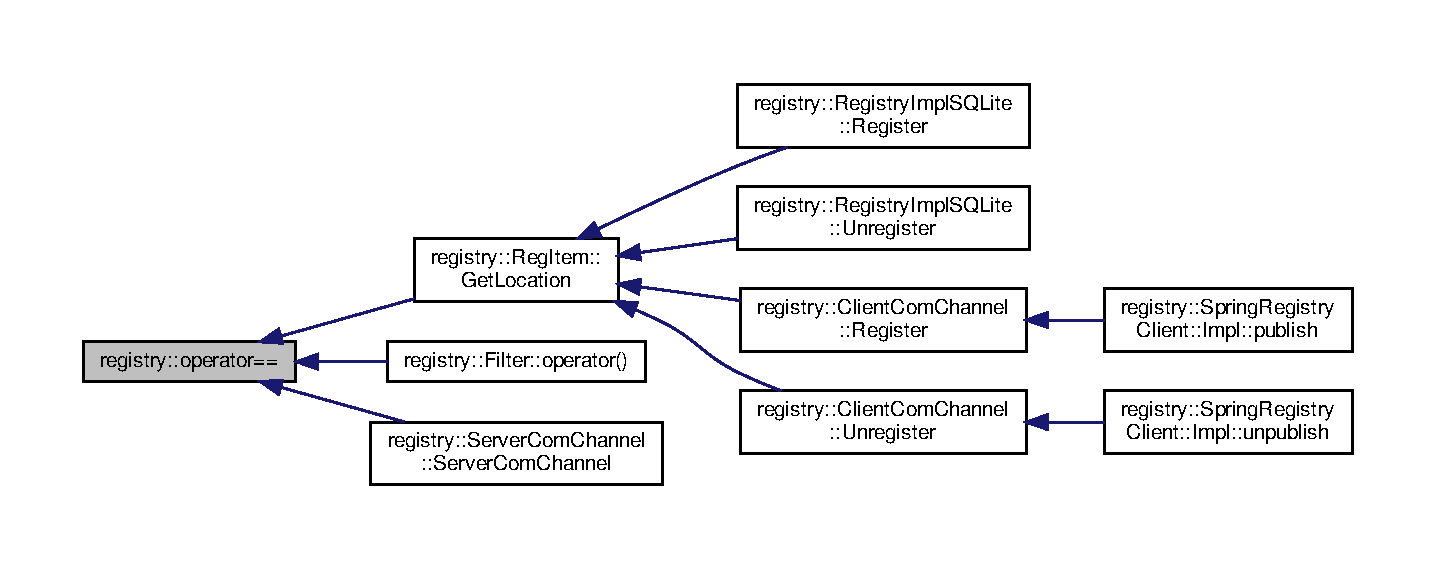
\includegraphics[width=350pt]{namespaceregistry_a3aea015bffedea5734787cec200bfe1b_icgraph}
\end{center}
\end{figure}
\mbox{\Hypertarget{namespaceregistry_af536cbf7e20589d15ebaef7741b96442}\label{namespaceregistry_af536cbf7e20589d15ebaef7741b96442}} 
\index{registry@{registry}!operator==@{operator==}}
\index{operator==@{operator==}!registry@{registry}}
\subsubsection{\texorpdfstring{operator==()}{operator==()}\hspace{0.1cm}{\footnotesize\ttfamily [3/3]}}
{\footnotesize\ttfamily bool registry\+::operator== (\begin{DoxyParamCaption}\item[{\hyperlink{classregistry_1_1Filter}{Filter} const \&}]{f1,  }\item[{\hyperlink{classregistry_1_1Filter}{Filter} const \&}]{f2 }\end{DoxyParamCaption})\hspace{0.3cm}{\ttfamily [inline]}}


\chapter{Class Documentation}
\hypertarget{classregistry_1_1AbstractRegistry}{}\section{registry\+:\+:Abstract\+Registry Class Reference}
\label{classregistry_1_1AbstractRegistry}\index{registry\+::\+Abstract\+Registry@{registry\+::\+Abstract\+Registry}}


The interface for Registry classes.  




{\ttfamily \#include $<$registry\+\_\+core.\+hpp$>$}



Inheritance diagram for registry\+:\+:Abstract\+Registry\+:
\nopagebreak
\begin{figure}[H]
\begin{center}
\leavevmode
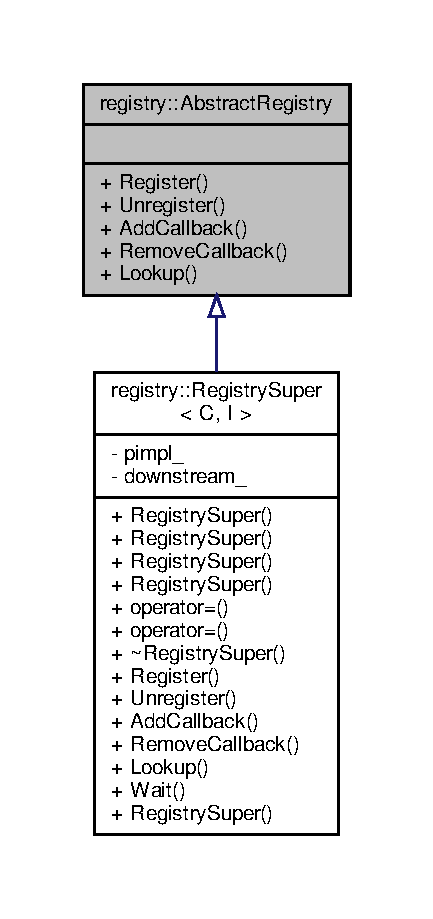
\includegraphics[width=208pt]{classregistry_1_1AbstractRegistry__inherit__graph}
\end{center}
\end{figure}


Collaboration diagram for registry\+:\+:Abstract\+Registry\+:\nopagebreak
\begin{figure}[H]
\begin{center}
\leavevmode
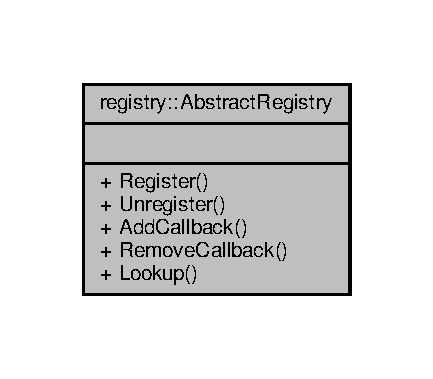
\includegraphics[width=208pt]{classregistry_1_1AbstractRegistry__coll__graph}
\end{center}
\end{figure}
\subsection*{Public Types}
\begin{DoxyCompactItemize}
\item 
using \hyperlink{classregistry_1_1AbstractRegistry_a08a798ca9ca1c4c983ebd2386ca3c315}{Callback} = std\+::function$<$ void(std\+::vector$<$ \hyperlink{classregistry_1_1RegItem}{Reg\+Item} $>$)$>$
\item 
using \hyperlink{classregistry_1_1AbstractRegistry_a31f6bef634dcd324efebaf55f99b950f}{Filter\+Callback} = std\+::tuple$<$ \hyperlink{classregistry_1_1Filter}{Filter}, \hyperlink{classregistry_1_1AbstractRegistry_a08a798ca9ca1c4c983ebd2386ca3c315}{Callback} $>$
\end{DoxyCompactItemize}
\subsection*{Public Member Functions}
\begin{DoxyCompactItemize}
\item 
virtual void \hyperlink{classregistry_1_1AbstractRegistry_a5deafe61aa33b1be6b261d815e7397a1}{Register} (\hyperlink{classregistry_1_1RegItem}{Reg\+Item} ri) noexcept=0
\item 
virtual void \hyperlink{classregistry_1_1AbstractRegistry_ac5bb3b6a75a63a474f6b0afb31ea51c1}{Unregister} (\hyperlink{classregistry_1_1RegItem}{Reg\+Item} ri) noexcept=0
\item 
virtual void \hyperlink{classregistry_1_1AbstractRegistry_a83f61ca483c22185ddf43653ca65a8ef}{Add\+Callback} (\hyperlink{classregistry_1_1Filter}{Filter} flt, \hyperlink{classregistry_1_1AbstractRegistry_a08a798ca9ca1c4c983ebd2386ca3c315}{Callback} cb) noexcept=0
\item 
virtual void \hyperlink{classregistry_1_1AbstractRegistry_ae09a4b165d916b6c212988d882d1a33f}{Remove\+Callback} (\hyperlink{classregistry_1_1Filter}{Filter} flt, \hyperlink{classregistry_1_1AbstractRegistry_a08a798ca9ca1c4c983ebd2386ca3c315}{Callback} cb) noexcept=0
\item 
virtual std\+::vector$<$ \hyperlink{classregistry_1_1RegItem}{Reg\+Item} $>$ \hyperlink{classregistry_1_1AbstractRegistry_a978d5b55eeea945b0cc441e28a084518}{Lookup} (\hyperlink{classregistry_1_1Filter}{Filter} flt) noexcept=0
\end{DoxyCompactItemize}


\subsection{Detailed Description}
The interface for Registry classes. 

\subsection{Member Typedef Documentation}
\mbox{\Hypertarget{classregistry_1_1AbstractRegistry_a08a798ca9ca1c4c983ebd2386ca3c315}\label{classregistry_1_1AbstractRegistry_a08a798ca9ca1c4c983ebd2386ca3c315}} 
\index{registry\+::\+Abstract\+Registry@{registry\+::\+Abstract\+Registry}!Callback@{Callback}}
\index{Callback@{Callback}!registry\+::\+Abstract\+Registry@{registry\+::\+Abstract\+Registry}}
\subsubsection{\texorpdfstring{Callback}{Callback}}
{\footnotesize\ttfamily using \hyperlink{classregistry_1_1AbstractRegistry_a08a798ca9ca1c4c983ebd2386ca3c315}{registry\+::\+Abstract\+Registry\+::\+Callback} =  std\+::function$<$void(std\+::vector$<$\hyperlink{classregistry_1_1RegItem}{Reg\+Item}$>$)$>$}

\mbox{\Hypertarget{classregistry_1_1AbstractRegistry_a31f6bef634dcd324efebaf55f99b950f}\label{classregistry_1_1AbstractRegistry_a31f6bef634dcd324efebaf55f99b950f}} 
\index{registry\+::\+Abstract\+Registry@{registry\+::\+Abstract\+Registry}!Filter\+Callback@{Filter\+Callback}}
\index{Filter\+Callback@{Filter\+Callback}!registry\+::\+Abstract\+Registry@{registry\+::\+Abstract\+Registry}}
\subsubsection{\texorpdfstring{Filter\+Callback}{FilterCallback}}
{\footnotesize\ttfamily using \hyperlink{classregistry_1_1AbstractRegistry_a31f6bef634dcd324efebaf55f99b950f}{registry\+::\+Abstract\+Registry\+::\+Filter\+Callback} =  std\+::tuple$<$\hyperlink{classregistry_1_1Filter}{Filter}, \hyperlink{classregistry_1_1AbstractRegistry_a08a798ca9ca1c4c983ebd2386ca3c315}{Callback}$>$}



\subsection{Member Function Documentation}
\mbox{\Hypertarget{classregistry_1_1AbstractRegistry_a83f61ca483c22185ddf43653ca65a8ef}\label{classregistry_1_1AbstractRegistry_a83f61ca483c22185ddf43653ca65a8ef}} 
\index{registry\+::\+Abstract\+Registry@{registry\+::\+Abstract\+Registry}!Add\+Callback@{Add\+Callback}}
\index{Add\+Callback@{Add\+Callback}!registry\+::\+Abstract\+Registry@{registry\+::\+Abstract\+Registry}}
\subsubsection{\texorpdfstring{Add\+Callback()}{AddCallback()}}
{\footnotesize\ttfamily virtual void registry\+::\+Abstract\+Registry\+::\+Add\+Callback (\begin{DoxyParamCaption}\item[{\hyperlink{classregistry_1_1Filter}{Filter}}]{flt,  }\item[{\hyperlink{classregistry_1_1AbstractRegistry_a08a798ca9ca1c4c983ebd2386ca3c315}{Callback}}]{cb }\end{DoxyParamCaption})\hspace{0.3cm}{\ttfamily [pure virtual]}, {\ttfamily [noexcept]}}



Implemented in \hyperlink{classregistry_1_1RegistrySuper_a80e234502449509e0c9ce75e787ef974}{registry\+::\+Registry\+Super$<$ C, I $>$}.

\mbox{\Hypertarget{classregistry_1_1AbstractRegistry_a978d5b55eeea945b0cc441e28a084518}\label{classregistry_1_1AbstractRegistry_a978d5b55eeea945b0cc441e28a084518}} 
\index{registry\+::\+Abstract\+Registry@{registry\+::\+Abstract\+Registry}!Lookup@{Lookup}}
\index{Lookup@{Lookup}!registry\+::\+Abstract\+Registry@{registry\+::\+Abstract\+Registry}}
\subsubsection{\texorpdfstring{Lookup()}{Lookup()}}
{\footnotesize\ttfamily virtual std\+::vector$<$\hyperlink{classregistry_1_1RegItem}{Reg\+Item}$>$ registry\+::\+Abstract\+Registry\+::\+Lookup (\begin{DoxyParamCaption}\item[{\hyperlink{classregistry_1_1Filter}{Filter}}]{flt }\end{DoxyParamCaption})\hspace{0.3cm}{\ttfamily [pure virtual]}, {\ttfamily [noexcept]}}



Implemented in \hyperlink{classregistry_1_1RegistrySuper_a83240eacc385688b32998c1e83d086c5}{registry\+::\+Registry\+Super$<$ C, I $>$}.

Here is the caller graph for this function\+:\nopagebreak
\begin{figure}[H]
\begin{center}
\leavevmode
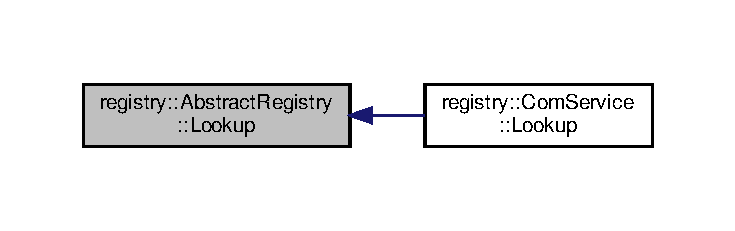
\includegraphics[width=350pt]{classregistry_1_1AbstractRegistry_a978d5b55eeea945b0cc441e28a084518_icgraph}
\end{center}
\end{figure}
\mbox{\Hypertarget{classregistry_1_1AbstractRegistry_a5deafe61aa33b1be6b261d815e7397a1}\label{classregistry_1_1AbstractRegistry_a5deafe61aa33b1be6b261d815e7397a1}} 
\index{registry\+::\+Abstract\+Registry@{registry\+::\+Abstract\+Registry}!Register@{Register}}
\index{Register@{Register}!registry\+::\+Abstract\+Registry@{registry\+::\+Abstract\+Registry}}
\subsubsection{\texorpdfstring{Register()}{Register()}}
{\footnotesize\ttfamily virtual void registry\+::\+Abstract\+Registry\+::\+Register (\begin{DoxyParamCaption}\item[{\hyperlink{classregistry_1_1RegItem}{Reg\+Item}}]{ri }\end{DoxyParamCaption})\hspace{0.3cm}{\ttfamily [pure virtual]}, {\ttfamily [noexcept]}}



Implemented in \hyperlink{classregistry_1_1RegistrySuper_a6293786807c1d9cc1f72a60c8c218b6f}{registry\+::\+Registry\+Super$<$ C, I $>$}.

Here is the caller graph for this function\+:\nopagebreak
\begin{figure}[H]
\begin{center}
\leavevmode
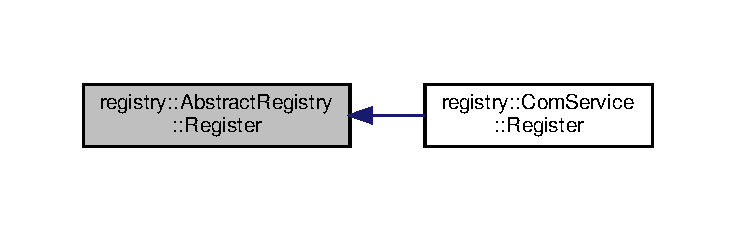
\includegraphics[width=350pt]{classregistry_1_1AbstractRegistry_a5deafe61aa33b1be6b261d815e7397a1_icgraph}
\end{center}
\end{figure}
\mbox{\Hypertarget{classregistry_1_1AbstractRegistry_ae09a4b165d916b6c212988d882d1a33f}\label{classregistry_1_1AbstractRegistry_ae09a4b165d916b6c212988d882d1a33f}} 
\index{registry\+::\+Abstract\+Registry@{registry\+::\+Abstract\+Registry}!Remove\+Callback@{Remove\+Callback}}
\index{Remove\+Callback@{Remove\+Callback}!registry\+::\+Abstract\+Registry@{registry\+::\+Abstract\+Registry}}
\subsubsection{\texorpdfstring{Remove\+Callback()}{RemoveCallback()}}
{\footnotesize\ttfamily virtual void registry\+::\+Abstract\+Registry\+::\+Remove\+Callback (\begin{DoxyParamCaption}\item[{\hyperlink{classregistry_1_1Filter}{Filter}}]{flt,  }\item[{\hyperlink{classregistry_1_1AbstractRegistry_a08a798ca9ca1c4c983ebd2386ca3c315}{Callback}}]{cb }\end{DoxyParamCaption})\hspace{0.3cm}{\ttfamily [pure virtual]}, {\ttfamily [noexcept]}}



Implemented in \hyperlink{classregistry_1_1RegistrySuper_a61948ba29418a844f1b2c9b1259e26bf}{registry\+::\+Registry\+Super$<$ C, I $>$}.

\mbox{\Hypertarget{classregistry_1_1AbstractRegistry_ac5bb3b6a75a63a474f6b0afb31ea51c1}\label{classregistry_1_1AbstractRegistry_ac5bb3b6a75a63a474f6b0afb31ea51c1}} 
\index{registry\+::\+Abstract\+Registry@{registry\+::\+Abstract\+Registry}!Unregister@{Unregister}}
\index{Unregister@{Unregister}!registry\+::\+Abstract\+Registry@{registry\+::\+Abstract\+Registry}}
\subsubsection{\texorpdfstring{Unregister()}{Unregister()}}
{\footnotesize\ttfamily virtual void registry\+::\+Abstract\+Registry\+::\+Unregister (\begin{DoxyParamCaption}\item[{\hyperlink{classregistry_1_1RegItem}{Reg\+Item}}]{ri }\end{DoxyParamCaption})\hspace{0.3cm}{\ttfamily [pure virtual]}, {\ttfamily [noexcept]}}



Implemented in \hyperlink{classregistry_1_1RegistrySuper_a3d35e055e1e69a00074701356e3e700f}{registry\+::\+Registry\+Super$<$ C, I $>$}.

Here is the caller graph for this function\+:\nopagebreak
\begin{figure}[H]
\begin{center}
\leavevmode
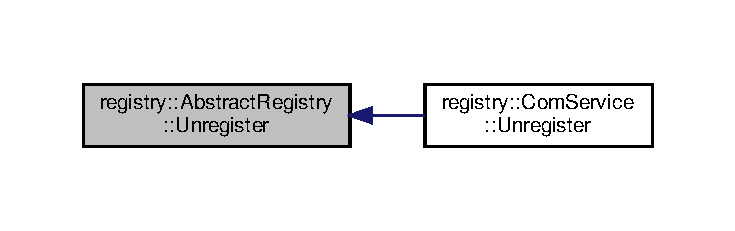
\includegraphics[width=350pt]{classregistry_1_1AbstractRegistry_ac5bb3b6a75a63a474f6b0afb31ea51c1_icgraph}
\end{center}
\end{figure}


The documentation for this class was generated from the following file\+:\begin{DoxyCompactItemize}
\item 
registry/src/\hyperlink{registry__core_8hpp}{registry\+\_\+core.\+hpp}\end{DoxyCompactItemize}

\hypertarget{structregistry_1_1BufferLocation}{}\section{registry\+:\+:Buffer\+Location Struct Reference}
\label{structregistry_1_1BufferLocation}\index{registry\+::\+Buffer\+Location@{registry\+::\+Buffer\+Location}}


{\ttfamily \#include $<$registry\+\_\+common.\+hpp$>$}



Collaboration diagram for registry\+:\+:Buffer\+Location\+:\nopagebreak
\begin{figure}[H]
\begin{center}
\leavevmode
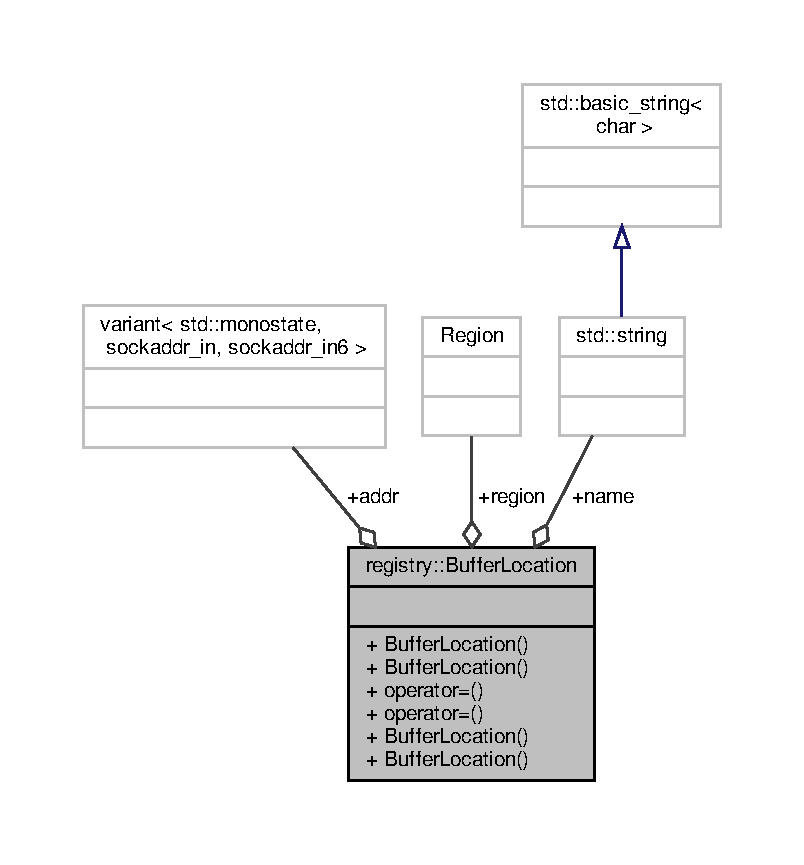
\includegraphics[width=350pt]{structregistry_1_1BufferLocation__coll__graph}
\end{center}
\end{figure}
\subsection*{Public Types}
\begin{DoxyCompactItemize}
\item 
enum \hyperlink{structregistry_1_1BufferLocation_a07b156ecd0690dbebb5cba36d4d23ba0}{Region} \{ \hyperlink{structregistry_1_1BufferLocation_a07b156ecd0690dbebb5cba36d4d23ba0aabe46bdcd661a69bbcbc5963274eee79}{k\+Near}, 
\hyperlink{structregistry_1_1BufferLocation_a07b156ecd0690dbebb5cba36d4d23ba0a7ff68b6384eccdda3bc530b02228102d}{k\+Far}
 \}\begin{DoxyCompactList}\small\item\em Supported types of ring buffers. \end{DoxyCompactList}
\item 
using \hyperlink{structregistry_1_1BufferLocation_ad3c2279012b74798fa1e348507020fa4}{Name\+Type} = std\+::string
\end{DoxyCompactItemize}
\subsection*{Public Member Functions}
\begin{DoxyCompactItemize}
\item 
\hyperlink{structregistry_1_1BufferLocation_a30830e0d0cfae8971273c57a894242d9}{Buffer\+Location} (\hyperlink{structregistry_1_1BufferLocation_ad3c2279012b74798fa1e348507020fa4}{Name\+Type} n) noexcept
\item 
\hyperlink{structregistry_1_1BufferLocation_a7e2e78fc0a567f47a9bb01e2d3683984}{Buffer\+Location} (\hyperlink{structregistry_1_1BufferLocation_ad3c2279012b74798fa1e348507020fa4}{Name\+Type} n, \hyperlink{namespaceregistry_a2d7eac31eb792025667bcebdfe93dbf2}{Net\+Addr} const \&\hyperlink{structregistry_1_1BufferLocation_ad22f3b9cd359ad88ad3ddcad69fdb740}{addr}) noexcept
\item 
\hyperlink{structregistry_1_1BufferLocation}{Buffer\+Location} \& \hyperlink{structregistry_1_1BufferLocation_a545aea2299f77c020043efc9da9ab697}{operator=} (\hyperlink{structregistry_1_1BufferLocation}{Buffer\+Location} const \&b)=default
\item 
\hyperlink{structregistry_1_1BufferLocation}{Buffer\+Location} \& \hyperlink{structregistry_1_1BufferLocation_ac20495af404297a191fc8f4ed869e7c0}{operator=} (\hyperlink{structregistry_1_1BufferLocation}{Buffer\+Location} \&\&b) noexcept=default
\item 
\hyperlink{structregistry_1_1BufferLocation_a13e370aa3a10d57ca0f7a3ab109f9405}{Buffer\+Location} (\hyperlink{structregistry_1_1BufferLocation}{Buffer\+Location} const \&b)=default
\item 
\hyperlink{structregistry_1_1BufferLocation_a64f5245e74c8d9e544dc19057bcc2798}{Buffer\+Location} (\hyperlink{structregistry_1_1BufferLocation}{Buffer\+Location} \&\&b) noexcept=default
\end{DoxyCompactItemize}
\subsection*{Public Attributes}
\begin{DoxyCompactItemize}
\item 
\hyperlink{structregistry_1_1BufferLocation_ad3c2279012b74798fa1e348507020fa4}{Name\+Type} \hyperlink{structregistry_1_1BufferLocation_a9941e0d8dceeb136a95c50bef3792082}{name}
\begin{DoxyCompactList}\small\item\em The name of this ring buffer that is being expoded. \end{DoxyCompactList}\item 
\hyperlink{structregistry_1_1BufferLocation_a07b156ecd0690dbebb5cba36d4d23ba0}{Region} \hyperlink{structregistry_1_1BufferLocation_ad05676e193d5259c84e53f7037ed3878}{region}
\item 
\hyperlink{namespaceregistry_a2d7eac31eb792025667bcebdfe93dbf2}{Net\+Addr} \hyperlink{structregistry_1_1BufferLocation_ad22f3b9cd359ad88ad3ddcad69fdb740}{addr}
\end{DoxyCompactItemize}


\subsection{Member Typedef Documentation}
\mbox{\Hypertarget{structregistry_1_1BufferLocation_ad3c2279012b74798fa1e348507020fa4}\label{structregistry_1_1BufferLocation_ad3c2279012b74798fa1e348507020fa4}} 
\index{registry\+::\+Buffer\+Location@{registry\+::\+Buffer\+Location}!Name\+Type@{Name\+Type}}
\index{Name\+Type@{Name\+Type}!registry\+::\+Buffer\+Location@{registry\+::\+Buffer\+Location}}
\subsubsection{\texorpdfstring{Name\+Type}{NameType}}
{\footnotesize\ttfamily using \hyperlink{structregistry_1_1BufferLocation_ad3c2279012b74798fa1e348507020fa4}{registry\+::\+Buffer\+Location\+::\+Name\+Type} =  std\+::string}



\subsection{Member Enumeration Documentation}
\mbox{\Hypertarget{structregistry_1_1BufferLocation_a07b156ecd0690dbebb5cba36d4d23ba0}\label{structregistry_1_1BufferLocation_a07b156ecd0690dbebb5cba36d4d23ba0}} 
\index{registry\+::\+Buffer\+Location@{registry\+::\+Buffer\+Location}!Region@{Region}}
\index{Region@{Region}!registry\+::\+Buffer\+Location@{registry\+::\+Buffer\+Location}}
\subsubsection{\texorpdfstring{Region}{Region}}
{\footnotesize\ttfamily enum \hyperlink{structregistry_1_1BufferLocation_a07b156ecd0690dbebb5cba36d4d23ba0}{registry\+::\+Buffer\+Location\+::\+Region}}



Supported types of ring buffers. 

\begin{DoxyEnumFields}{Enumerator}
\raisebox{\heightof{T}}[0pt][0pt]{\index{k\+Near@{k\+Near}!registry\+::\+Buffer\+Location@{registry\+::\+Buffer\+Location}}\index{registry\+::\+Buffer\+Location@{registry\+::\+Buffer\+Location}!k\+Near@{k\+Near}}}\mbox{\Hypertarget{structregistry_1_1BufferLocation_a07b156ecd0690dbebb5cba36d4d23ba0aabe46bdcd661a69bbcbc5963274eee79}\label{structregistry_1_1BufferLocation_a07b156ecd0690dbebb5cba36d4d23ba0aabe46bdcd661a69bbcbc5963274eee79}} 
k\+Near&The buffer resides on the system computer as the client. \\
\hline

\raisebox{\heightof{T}}[0pt][0pt]{\index{k\+Far@{k\+Far}!registry\+::\+Buffer\+Location@{registry\+::\+Buffer\+Location}}\index{registry\+::\+Buffer\+Location@{registry\+::\+Buffer\+Location}!k\+Far@{k\+Far}}}\mbox{\Hypertarget{structregistry_1_1BufferLocation_a07b156ecd0690dbebb5cba36d4d23ba0a7ff68b6384eccdda3bc530b02228102d}\label{structregistry_1_1BufferLocation_a07b156ecd0690dbebb5cba36d4d23ba0a7ff68b6384eccdda3bc530b02228102d}} 
k\+Far&The buffer resides on a remote system and should be accessed over a network. \\
\hline

\end{DoxyEnumFields}


\subsection{Constructor \& Destructor Documentation}
\mbox{\Hypertarget{structregistry_1_1BufferLocation_a30830e0d0cfae8971273c57a894242d9}\label{structregistry_1_1BufferLocation_a30830e0d0cfae8971273c57a894242d9}} 
\index{registry\+::\+Buffer\+Location@{registry\+::\+Buffer\+Location}!Buffer\+Location@{Buffer\+Location}}
\index{Buffer\+Location@{Buffer\+Location}!registry\+::\+Buffer\+Location@{registry\+::\+Buffer\+Location}}
\subsubsection{\texorpdfstring{Buffer\+Location()}{BufferLocation()}\hspace{0.1cm}{\footnotesize\ttfamily [1/4]}}
{\footnotesize\ttfamily registry\+::\+Buffer\+Location\+::\+Buffer\+Location (\begin{DoxyParamCaption}\item[{\hyperlink{structregistry_1_1BufferLocation_ad3c2279012b74798fa1e348507020fa4}{Name\+Type}}]{n }\end{DoxyParamCaption})\hspace{0.3cm}{\ttfamily [inline]}, {\ttfamily [noexcept]}}

Here is the caller graph for this function\+:\nopagebreak
\begin{figure}[H]
\begin{center}
\leavevmode
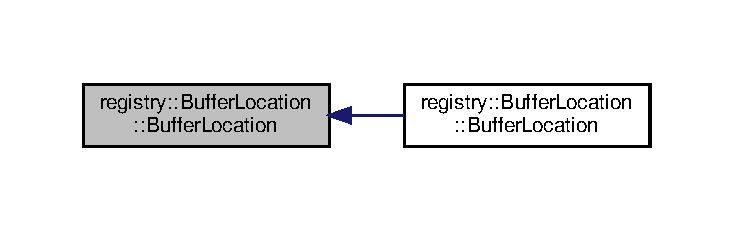
\includegraphics[width=350pt]{structregistry_1_1BufferLocation_a30830e0d0cfae8971273c57a894242d9_icgraph}
\end{center}
\end{figure}
\mbox{\Hypertarget{structregistry_1_1BufferLocation_a7e2e78fc0a567f47a9bb01e2d3683984}\label{structregistry_1_1BufferLocation_a7e2e78fc0a567f47a9bb01e2d3683984}} 
\index{registry\+::\+Buffer\+Location@{registry\+::\+Buffer\+Location}!Buffer\+Location@{Buffer\+Location}}
\index{Buffer\+Location@{Buffer\+Location}!registry\+::\+Buffer\+Location@{registry\+::\+Buffer\+Location}}
\subsubsection{\texorpdfstring{Buffer\+Location()}{BufferLocation()}\hspace{0.1cm}{\footnotesize\ttfamily [2/4]}}
{\footnotesize\ttfamily registry\+::\+Buffer\+Location\+::\+Buffer\+Location (\begin{DoxyParamCaption}\item[{\hyperlink{structregistry_1_1BufferLocation_ad3c2279012b74798fa1e348507020fa4}{Name\+Type}}]{n,  }\item[{\hyperlink{namespaceregistry_a2d7eac31eb792025667bcebdfe93dbf2}{Net\+Addr} const \&}]{addr }\end{DoxyParamCaption})\hspace{0.3cm}{\ttfamily [inline]}, {\ttfamily [noexcept]}}

Here is the call graph for this function\+:\nopagebreak
\begin{figure}[H]
\begin{center}
\leavevmode
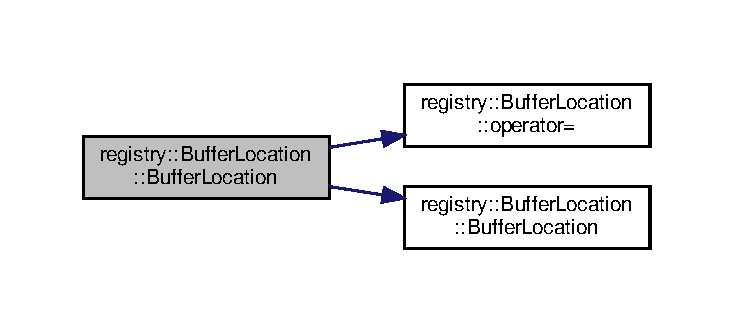
\includegraphics[width=350pt]{structregistry_1_1BufferLocation_a7e2e78fc0a567f47a9bb01e2d3683984_cgraph}
\end{center}
\end{figure}
\mbox{\Hypertarget{structregistry_1_1BufferLocation_a13e370aa3a10d57ca0f7a3ab109f9405}\label{structregistry_1_1BufferLocation_a13e370aa3a10d57ca0f7a3ab109f9405}} 
\index{registry\+::\+Buffer\+Location@{registry\+::\+Buffer\+Location}!Buffer\+Location@{Buffer\+Location}}
\index{Buffer\+Location@{Buffer\+Location}!registry\+::\+Buffer\+Location@{registry\+::\+Buffer\+Location}}
\subsubsection{\texorpdfstring{Buffer\+Location()}{BufferLocation()}\hspace{0.1cm}{\footnotesize\ttfamily [3/4]}}
{\footnotesize\ttfamily registry\+::\+Buffer\+Location\+::\+Buffer\+Location (\begin{DoxyParamCaption}\item[{\hyperlink{structregistry_1_1BufferLocation}{Buffer\+Location} const \&}]{b }\end{DoxyParamCaption})\hspace{0.3cm}{\ttfamily [default]}}

\mbox{\Hypertarget{structregistry_1_1BufferLocation_a64f5245e74c8d9e544dc19057bcc2798}\label{structregistry_1_1BufferLocation_a64f5245e74c8d9e544dc19057bcc2798}} 
\index{registry\+::\+Buffer\+Location@{registry\+::\+Buffer\+Location}!Buffer\+Location@{Buffer\+Location}}
\index{Buffer\+Location@{Buffer\+Location}!registry\+::\+Buffer\+Location@{registry\+::\+Buffer\+Location}}
\subsubsection{\texorpdfstring{Buffer\+Location()}{BufferLocation()}\hspace{0.1cm}{\footnotesize\ttfamily [4/4]}}
{\footnotesize\ttfamily registry\+::\+Buffer\+Location\+::\+Buffer\+Location (\begin{DoxyParamCaption}\item[{\hyperlink{structregistry_1_1BufferLocation}{Buffer\+Location} \&\&}]{b }\end{DoxyParamCaption})\hspace{0.3cm}{\ttfamily [default]}, {\ttfamily [noexcept]}}



\subsection{Member Function Documentation}
\mbox{\Hypertarget{structregistry_1_1BufferLocation_a545aea2299f77c020043efc9da9ab697}\label{structregistry_1_1BufferLocation_a545aea2299f77c020043efc9da9ab697}} 
\index{registry\+::\+Buffer\+Location@{registry\+::\+Buffer\+Location}!operator=@{operator=}}
\index{operator=@{operator=}!registry\+::\+Buffer\+Location@{registry\+::\+Buffer\+Location}}
\subsubsection{\texorpdfstring{operator=()}{operator=()}\hspace{0.1cm}{\footnotesize\ttfamily [1/2]}}
{\footnotesize\ttfamily \hyperlink{structregistry_1_1BufferLocation}{Buffer\+Location}\& registry\+::\+Buffer\+Location\+::operator= (\begin{DoxyParamCaption}\item[{\hyperlink{structregistry_1_1BufferLocation}{Buffer\+Location} const \&}]{b }\end{DoxyParamCaption})\hspace{0.3cm}{\ttfamily [default]}}

Here is the caller graph for this function\+:\nopagebreak
\begin{figure}[H]
\begin{center}
\leavevmode
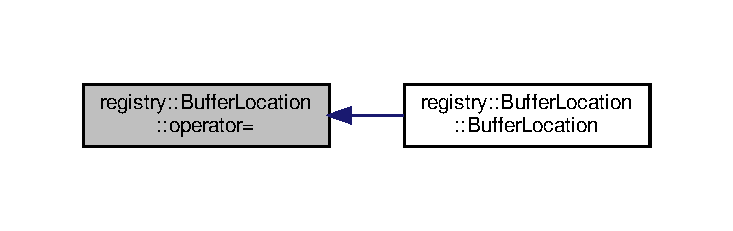
\includegraphics[width=350pt]{structregistry_1_1BufferLocation_a545aea2299f77c020043efc9da9ab697_icgraph}
\end{center}
\end{figure}
\mbox{\Hypertarget{structregistry_1_1BufferLocation_ac20495af404297a191fc8f4ed869e7c0}\label{structregistry_1_1BufferLocation_ac20495af404297a191fc8f4ed869e7c0}} 
\index{registry\+::\+Buffer\+Location@{registry\+::\+Buffer\+Location}!operator=@{operator=}}
\index{operator=@{operator=}!registry\+::\+Buffer\+Location@{registry\+::\+Buffer\+Location}}
\subsubsection{\texorpdfstring{operator=()}{operator=()}\hspace{0.1cm}{\footnotesize\ttfamily [2/2]}}
{\footnotesize\ttfamily \hyperlink{structregistry_1_1BufferLocation}{Buffer\+Location}\& registry\+::\+Buffer\+Location\+::operator= (\begin{DoxyParamCaption}\item[{\hyperlink{structregistry_1_1BufferLocation}{Buffer\+Location} \&\&}]{b }\end{DoxyParamCaption})\hspace{0.3cm}{\ttfamily [default]}, {\ttfamily [noexcept]}}



\subsection{Member Data Documentation}
\mbox{\Hypertarget{structregistry_1_1BufferLocation_ad22f3b9cd359ad88ad3ddcad69fdb740}\label{structregistry_1_1BufferLocation_ad22f3b9cd359ad88ad3ddcad69fdb740}} 
\index{registry\+::\+Buffer\+Location@{registry\+::\+Buffer\+Location}!addr@{addr}}
\index{addr@{addr}!registry\+::\+Buffer\+Location@{registry\+::\+Buffer\+Location}}
\subsubsection{\texorpdfstring{addr}{addr}}
{\footnotesize\ttfamily \hyperlink{namespaceregistry_a2d7eac31eb792025667bcebdfe93dbf2}{Net\+Addr} registry\+::\+Buffer\+Location\+::addr}

The \hyperlink{classNetAddr}{Net\+Addr} describing the location of this \hyperlink{structregistry_1_1BufferLocation}{Buffer\+Location} with respect to the Registry. \mbox{\Hypertarget{structregistry_1_1BufferLocation_a9941e0d8dceeb136a95c50bef3792082}\label{structregistry_1_1BufferLocation_a9941e0d8dceeb136a95c50bef3792082}} 
\index{registry\+::\+Buffer\+Location@{registry\+::\+Buffer\+Location}!name@{name}}
\index{name@{name}!registry\+::\+Buffer\+Location@{registry\+::\+Buffer\+Location}}
\subsubsection{\texorpdfstring{name}{name}}
{\footnotesize\ttfamily \hyperlink{structregistry_1_1BufferLocation_ad3c2279012b74798fa1e348507020fa4}{Name\+Type} registry\+::\+Buffer\+Location\+::name}



The name of this ring buffer that is being expoded. 

\mbox{\Hypertarget{structregistry_1_1BufferLocation_ad05676e193d5259c84e53f7037ed3878}\label{structregistry_1_1BufferLocation_ad05676e193d5259c84e53f7037ed3878}} 
\index{registry\+::\+Buffer\+Location@{registry\+::\+Buffer\+Location}!region@{region}}
\index{region@{region}!registry\+::\+Buffer\+Location@{registry\+::\+Buffer\+Location}}
\subsubsection{\texorpdfstring{region}{region}}
{\footnotesize\ttfamily \hyperlink{structregistry_1_1BufferLocation_a07b156ecd0690dbebb5cba36d4d23ba0}{Region} registry\+::\+Buffer\+Location\+::region}

The Region of this buffer location with respect to a given Registry. 

The documentation for this struct was generated from the following file\+:\begin{DoxyCompactItemize}
\item 
registry/include/\hyperlink{registry__common_8hpp}{registry\+\_\+common.\+hpp}\end{DoxyCompactItemize}

\hypertarget{structChannelNotFound}{}\section{Channel\+Not\+Found Struct Reference}
\label{structChannelNotFound}\index{Channel\+Not\+Found@{Channel\+Not\+Found}}


{\ttfamily \#include $<$extractor\+\_\+common.\+hpp$>$}



Inheritance diagram for Channel\+Not\+Found\+:\nopagebreak
\begin{figure}[H]
\begin{center}
\leavevmode
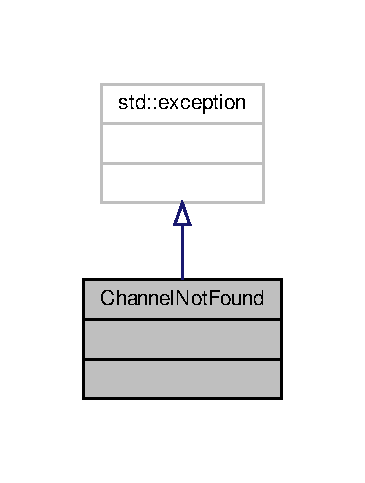
\includegraphics[width=175pt]{structChannelNotFound__inherit__graph}
\end{center}
\end{figure}


Collaboration diagram for Channel\+Not\+Found\+:\nopagebreak
\begin{figure}[H]
\begin{center}
\leavevmode
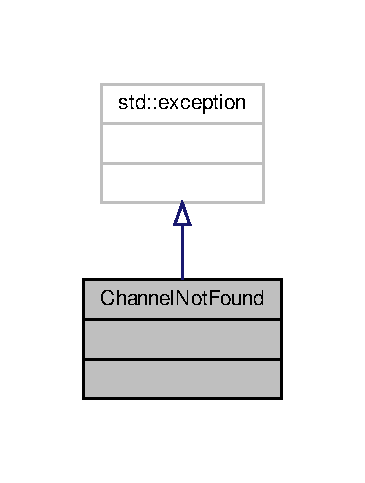
\includegraphics[width=175pt]{structChannelNotFound__coll__graph}
\end{center}
\end{figure}


The documentation for this struct was generated from the following file\+:\begin{DoxyCompactItemize}
\item 
extractor/include/\hyperlink{extractor__common_8hpp}{extractor\+\_\+common.\+hpp}\end{DoxyCompactItemize}

\hypertarget{classregistry_1_1ClientComChannel}{}\section{registry\+:\+:Client\+Com\+Channel Class Reference}
\label{classregistry_1_1ClientComChannel}\index{registry\+::\+Client\+Com\+Channel@{registry\+::\+Client\+Com\+Channel}}


This is a proxy that allows Registry clients to use its services remotly. This is actually a wrapper for the g\+R\+PC service stub.  




{\ttfamily \#include $<$registry\+\_\+core.\+hpp$>$}



Collaboration diagram for registry\+:\+:Client\+Com\+Channel\+:\nopagebreak
\begin{figure}[H]
\begin{center}
\leavevmode
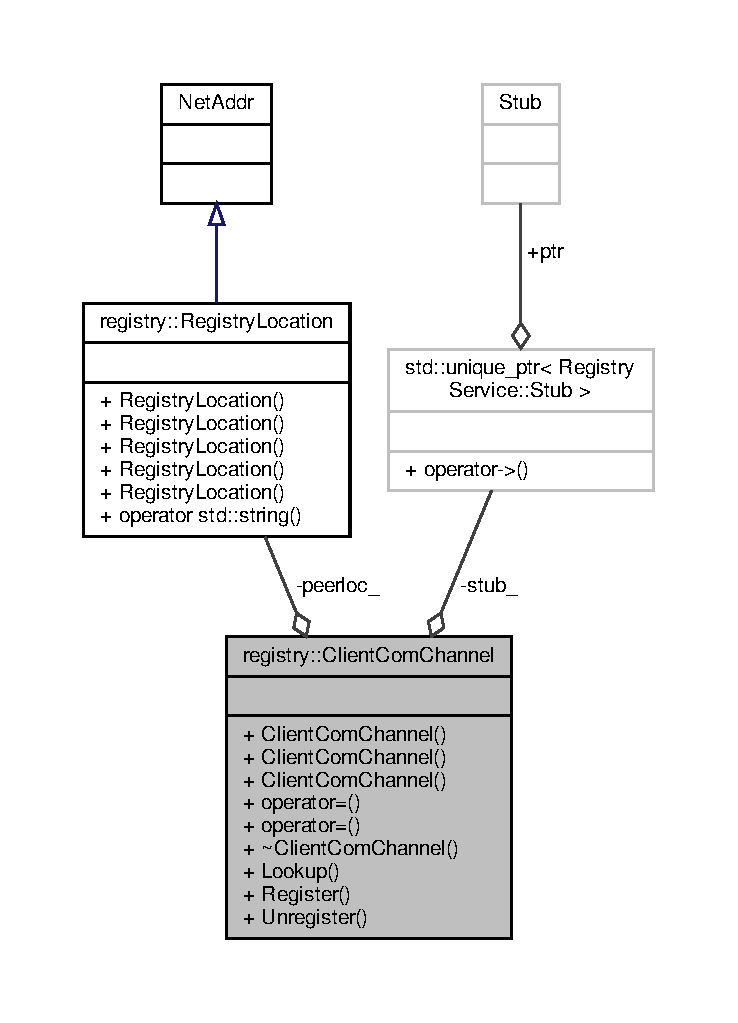
\includegraphics[width=350pt]{classregistry_1_1ClientComChannel__coll__graph}
\end{center}
\end{figure}
\subsection*{Public Member Functions}
\begin{DoxyCompactItemize}
\item 
\hyperlink{classregistry_1_1ClientComChannel_a5c2b0bc24a8b841c3a713dc9575a0917}{Client\+Com\+Channel} (\hyperlink{structregistry_1_1RegistryLocation}{Registry\+Location} const \&l) noexcept
\item 
\hyperlink{classregistry_1_1ClientComChannel_acbda0cc868a2dbfb8070688b758ca8b2}{Client\+Com\+Channel} (\hyperlink{classregistry_1_1ClientComChannel}{Client\+Com\+Channel} const \&)=delete
\item 
\hyperlink{classregistry_1_1ClientComChannel_a6af8524e3b31d52df3e28d0da71d5dee}{Client\+Com\+Channel} (\hyperlink{classregistry_1_1ClientComChannel}{Client\+Com\+Channel} const \&\&)=delete
\item 
\hyperlink{classregistry_1_1ClientComChannel}{Client\+Com\+Channel} \& \hyperlink{classregistry_1_1ClientComChannel_a70bdd7f48a91b7f6c4cf226f9203efbe}{operator=} (\hyperlink{classregistry_1_1ClientComChannel}{Client\+Com\+Channel} const \&)=delete
\item 
\hyperlink{classregistry_1_1ClientComChannel}{Client\+Com\+Channel} \& \hyperlink{classregistry_1_1ClientComChannel_ac3572b1e8e9edd73fe7717186ce41ef6}{operator=} (\hyperlink{classregistry_1_1ClientComChannel}{Client\+Com\+Channel} const \&\&)=delete
\item 
\hyperlink{classregistry_1_1ClientComChannel_a7e10fd32266882e6c18731533a7dc2b6}{$\sim$\+Client\+Com\+Channel} () noexcept=default
\item 
std\+::vector$<$ \hyperlink{classregistry_1_1RegItem}{Reg\+Item} $>$ \hyperlink{classregistry_1_1ClientComChannel_a564ba5480214a74c5697120084cafb54}{Lookup} (\hyperlink{classregistry_1_1Filter}{Filter} const \&filter) const
\item 
void \hyperlink{classregistry_1_1ClientComChannel_ad5566f6f10790d9090975c5be8916d40}{Register} (\hyperlink{classregistry_1_1RegItem}{Reg\+Item} const \&reg\+\_\+item) const
\item 
void \hyperlink{classregistry_1_1ClientComChannel_a74566850580e7071fb6ec0f1f0498d05}{Unregister} (\hyperlink{classregistry_1_1RegItem}{Reg\+Item} const \&reg\+\_\+item) const
\end{DoxyCompactItemize}
\subsection*{Private Attributes}
\begin{DoxyCompactItemize}
\item 
\hyperlink{structregistry_1_1RegistryLocation}{Registry\+Location} \hyperlink{classregistry_1_1ClientComChannel_ac59fe755362be649e2ec1ee555d2ead8}{peerloc\+\_\+}
\begin{DoxyCompactList}\small\item\em Location of the registry. \end{DoxyCompactList}\item 
std\+::unique\+\_\+ptr$<$ Registry\+Service\+::\+Stub $>$ \hyperlink{classregistry_1_1ClientComChannel_a92638fd8f461be8b5ef5a3a6c3a429ac}{stub\+\_\+}
\begin{DoxyCompactList}\small\item\em Client-\/side g\+R\+PC service stub. \end{DoxyCompactList}\end{DoxyCompactItemize}


\subsection{Detailed Description}
This is a proxy that allows Registry clients to use its services remotly. This is actually a wrapper for the g\+R\+PC service stub. 

\subsection{Constructor \& Destructor Documentation}
\mbox{\Hypertarget{classregistry_1_1ClientComChannel_a5c2b0bc24a8b841c3a713dc9575a0917}\label{classregistry_1_1ClientComChannel_a5c2b0bc24a8b841c3a713dc9575a0917}} 
\index{registry\+::\+Client\+Com\+Channel@{registry\+::\+Client\+Com\+Channel}!Client\+Com\+Channel@{Client\+Com\+Channel}}
\index{Client\+Com\+Channel@{Client\+Com\+Channel}!registry\+::\+Client\+Com\+Channel@{registry\+::\+Client\+Com\+Channel}}
\subsubsection{\texorpdfstring{Client\+Com\+Channel()}{ClientComChannel()}\hspace{0.1cm}{\footnotesize\ttfamily [1/3]}}
{\footnotesize\ttfamily registry\+::\+Client\+Com\+Channel\+::\+Client\+Com\+Channel (\begin{DoxyParamCaption}\item[{\hyperlink{structregistry_1_1RegistryLocation}{Registry\+Location} const \&}]{l }\end{DoxyParamCaption})\hspace{0.3cm}{\ttfamily [inline]}, {\ttfamily [noexcept]}}

\mbox{\Hypertarget{classregistry_1_1ClientComChannel_acbda0cc868a2dbfb8070688b758ca8b2}\label{classregistry_1_1ClientComChannel_acbda0cc868a2dbfb8070688b758ca8b2}} 
\index{registry\+::\+Client\+Com\+Channel@{registry\+::\+Client\+Com\+Channel}!Client\+Com\+Channel@{Client\+Com\+Channel}}
\index{Client\+Com\+Channel@{Client\+Com\+Channel}!registry\+::\+Client\+Com\+Channel@{registry\+::\+Client\+Com\+Channel}}
\subsubsection{\texorpdfstring{Client\+Com\+Channel()}{ClientComChannel()}\hspace{0.1cm}{\footnotesize\ttfamily [2/3]}}
{\footnotesize\ttfamily registry\+::\+Client\+Com\+Channel\+::\+Client\+Com\+Channel (\begin{DoxyParamCaption}\item[{\hyperlink{classregistry_1_1ClientComChannel}{Client\+Com\+Channel} const \&}]{ }\end{DoxyParamCaption})\hspace{0.3cm}{\ttfamily [delete]}}

\mbox{\Hypertarget{classregistry_1_1ClientComChannel_a6af8524e3b31d52df3e28d0da71d5dee}\label{classregistry_1_1ClientComChannel_a6af8524e3b31d52df3e28d0da71d5dee}} 
\index{registry\+::\+Client\+Com\+Channel@{registry\+::\+Client\+Com\+Channel}!Client\+Com\+Channel@{Client\+Com\+Channel}}
\index{Client\+Com\+Channel@{Client\+Com\+Channel}!registry\+::\+Client\+Com\+Channel@{registry\+::\+Client\+Com\+Channel}}
\subsubsection{\texorpdfstring{Client\+Com\+Channel()}{ClientComChannel()}\hspace{0.1cm}{\footnotesize\ttfamily [3/3]}}
{\footnotesize\ttfamily registry\+::\+Client\+Com\+Channel\+::\+Client\+Com\+Channel (\begin{DoxyParamCaption}\item[{\hyperlink{classregistry_1_1ClientComChannel}{Client\+Com\+Channel} const \&\&}]{ }\end{DoxyParamCaption})\hspace{0.3cm}{\ttfamily [delete]}}

\mbox{\Hypertarget{classregistry_1_1ClientComChannel_a7e10fd32266882e6c18731533a7dc2b6}\label{classregistry_1_1ClientComChannel_a7e10fd32266882e6c18731533a7dc2b6}} 
\index{registry\+::\+Client\+Com\+Channel@{registry\+::\+Client\+Com\+Channel}!````~Client\+Com\+Channel@{$\sim$\+Client\+Com\+Channel}}
\index{````~Client\+Com\+Channel@{$\sim$\+Client\+Com\+Channel}!registry\+::\+Client\+Com\+Channel@{registry\+::\+Client\+Com\+Channel}}
\subsubsection{\texorpdfstring{$\sim$\+Client\+Com\+Channel()}{~ClientComChannel()}}
{\footnotesize\ttfamily registry\+::\+Client\+Com\+Channel\+::$\sim$\+Client\+Com\+Channel (\begin{DoxyParamCaption}{ }\end{DoxyParamCaption})\hspace{0.3cm}{\ttfamily [default]}, {\ttfamily [noexcept]}}



\subsection{Member Function Documentation}
\mbox{\Hypertarget{classregistry_1_1ClientComChannel_a564ba5480214a74c5697120084cafb54}\label{classregistry_1_1ClientComChannel_a564ba5480214a74c5697120084cafb54}} 
\index{registry\+::\+Client\+Com\+Channel@{registry\+::\+Client\+Com\+Channel}!Lookup@{Lookup}}
\index{Lookup@{Lookup}!registry\+::\+Client\+Com\+Channel@{registry\+::\+Client\+Com\+Channel}}
\subsubsection{\texorpdfstring{Lookup()}{Lookup()}}
{\footnotesize\ttfamily std\+::vector$<$\hyperlink{classregistry_1_1RegItem}{Reg\+Item}$>$ registry\+::\+Client\+Com\+Channel\+::\+Lookup (\begin{DoxyParamCaption}\item[{\hyperlink{classregistry_1_1Filter}{Filter} const \&}]{filter }\end{DoxyParamCaption}) const\hspace{0.3cm}{\ttfamily [inline]}}

Here is the call graph for this function\+:
\nopagebreak
\begin{figure}[H]
\begin{center}
\leavevmode
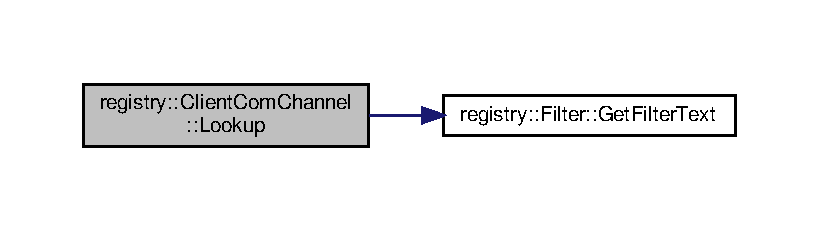
\includegraphics[width=350pt]{classregistry_1_1ClientComChannel_a564ba5480214a74c5697120084cafb54_cgraph}
\end{center}
\end{figure}
Here is the caller graph for this function\+:\nopagebreak
\begin{figure}[H]
\begin{center}
\leavevmode
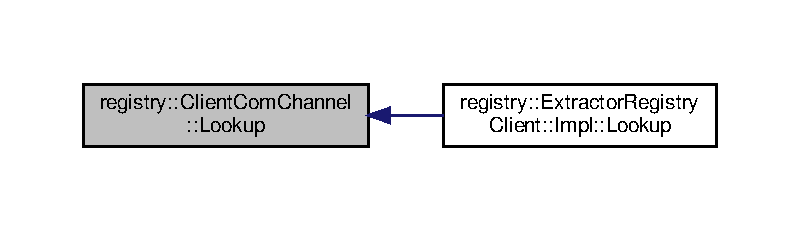
\includegraphics[width=350pt]{classregistry_1_1ClientComChannel_a564ba5480214a74c5697120084cafb54_icgraph}
\end{center}
\end{figure}
\mbox{\Hypertarget{classregistry_1_1ClientComChannel_a70bdd7f48a91b7f6c4cf226f9203efbe}\label{classregistry_1_1ClientComChannel_a70bdd7f48a91b7f6c4cf226f9203efbe}} 
\index{registry\+::\+Client\+Com\+Channel@{registry\+::\+Client\+Com\+Channel}!operator=@{operator=}}
\index{operator=@{operator=}!registry\+::\+Client\+Com\+Channel@{registry\+::\+Client\+Com\+Channel}}
\subsubsection{\texorpdfstring{operator=()}{operator=()}\hspace{0.1cm}{\footnotesize\ttfamily [1/2]}}
{\footnotesize\ttfamily \hyperlink{classregistry_1_1ClientComChannel}{Client\+Com\+Channel}\& registry\+::\+Client\+Com\+Channel\+::operator= (\begin{DoxyParamCaption}\item[{\hyperlink{classregistry_1_1ClientComChannel}{Client\+Com\+Channel} const \&}]{ }\end{DoxyParamCaption})\hspace{0.3cm}{\ttfamily [delete]}}

\mbox{\Hypertarget{classregistry_1_1ClientComChannel_ac3572b1e8e9edd73fe7717186ce41ef6}\label{classregistry_1_1ClientComChannel_ac3572b1e8e9edd73fe7717186ce41ef6}} 
\index{registry\+::\+Client\+Com\+Channel@{registry\+::\+Client\+Com\+Channel}!operator=@{operator=}}
\index{operator=@{operator=}!registry\+::\+Client\+Com\+Channel@{registry\+::\+Client\+Com\+Channel}}
\subsubsection{\texorpdfstring{operator=()}{operator=()}\hspace{0.1cm}{\footnotesize\ttfamily [2/2]}}
{\footnotesize\ttfamily \hyperlink{classregistry_1_1ClientComChannel}{Client\+Com\+Channel}\& registry\+::\+Client\+Com\+Channel\+::operator= (\begin{DoxyParamCaption}\item[{\hyperlink{classregistry_1_1ClientComChannel}{Client\+Com\+Channel} const \&\&}]{ }\end{DoxyParamCaption})\hspace{0.3cm}{\ttfamily [delete]}}

\mbox{\Hypertarget{classregistry_1_1ClientComChannel_ad5566f6f10790d9090975c5be8916d40}\label{classregistry_1_1ClientComChannel_ad5566f6f10790d9090975c5be8916d40}} 
\index{registry\+::\+Client\+Com\+Channel@{registry\+::\+Client\+Com\+Channel}!Register@{Register}}
\index{Register@{Register}!registry\+::\+Client\+Com\+Channel@{registry\+::\+Client\+Com\+Channel}}
\subsubsection{\texorpdfstring{Register()}{Register()}}
{\footnotesize\ttfamily void registry\+::\+Client\+Com\+Channel\+::\+Register (\begin{DoxyParamCaption}\item[{\hyperlink{classregistry_1_1RegItem}{Reg\+Item} const \&}]{reg\+\_\+item }\end{DoxyParamCaption}) const\hspace{0.3cm}{\ttfamily [inline]}}

Here is the call graph for this function\+:
\nopagebreak
\begin{figure}[H]
\begin{center}
\leavevmode
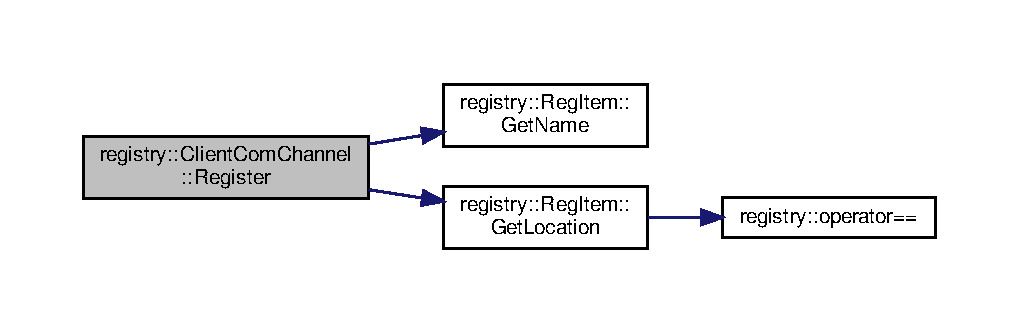
\includegraphics[width=350pt]{classregistry_1_1ClientComChannel_ad5566f6f10790d9090975c5be8916d40_cgraph}
\end{center}
\end{figure}
Here is the caller graph for this function\+:\nopagebreak
\begin{figure}[H]
\begin{center}
\leavevmode
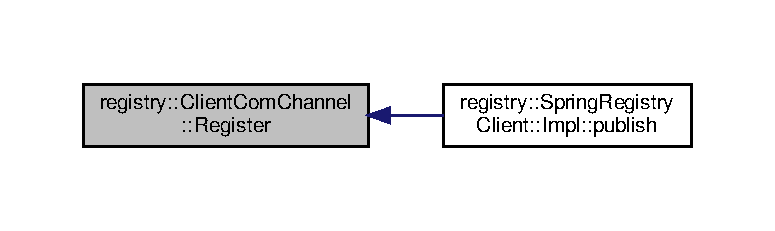
\includegraphics[width=350pt]{classregistry_1_1ClientComChannel_ad5566f6f10790d9090975c5be8916d40_icgraph}
\end{center}
\end{figure}
\mbox{\Hypertarget{classregistry_1_1ClientComChannel_a74566850580e7071fb6ec0f1f0498d05}\label{classregistry_1_1ClientComChannel_a74566850580e7071fb6ec0f1f0498d05}} 
\index{registry\+::\+Client\+Com\+Channel@{registry\+::\+Client\+Com\+Channel}!Unregister@{Unregister}}
\index{Unregister@{Unregister}!registry\+::\+Client\+Com\+Channel@{registry\+::\+Client\+Com\+Channel}}
\subsubsection{\texorpdfstring{Unregister()}{Unregister()}}
{\footnotesize\ttfamily void registry\+::\+Client\+Com\+Channel\+::\+Unregister (\begin{DoxyParamCaption}\item[{\hyperlink{classregistry_1_1RegItem}{Reg\+Item} const \&}]{reg\+\_\+item }\end{DoxyParamCaption}) const\hspace{0.3cm}{\ttfamily [inline]}}

Here is the call graph for this function\+:
\nopagebreak
\begin{figure}[H]
\begin{center}
\leavevmode
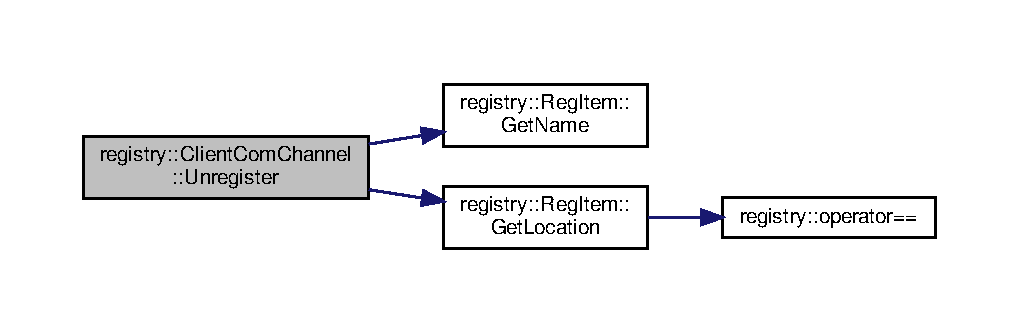
\includegraphics[width=350pt]{classregistry_1_1ClientComChannel_a74566850580e7071fb6ec0f1f0498d05_cgraph}
\end{center}
\end{figure}
Here is the caller graph for this function\+:\nopagebreak
\begin{figure}[H]
\begin{center}
\leavevmode
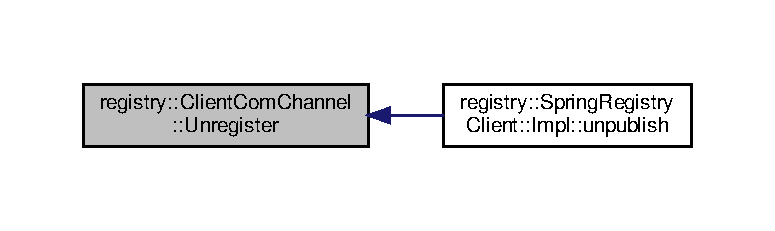
\includegraphics[width=350pt]{classregistry_1_1ClientComChannel_a74566850580e7071fb6ec0f1f0498d05_icgraph}
\end{center}
\end{figure}


\subsection{Member Data Documentation}
\mbox{\Hypertarget{classregistry_1_1ClientComChannel_ac59fe755362be649e2ec1ee555d2ead8}\label{classregistry_1_1ClientComChannel_ac59fe755362be649e2ec1ee555d2ead8}} 
\index{registry\+::\+Client\+Com\+Channel@{registry\+::\+Client\+Com\+Channel}!peerloc\+\_\+@{peerloc\+\_\+}}
\index{peerloc\+\_\+@{peerloc\+\_\+}!registry\+::\+Client\+Com\+Channel@{registry\+::\+Client\+Com\+Channel}}
\subsubsection{\texorpdfstring{peerloc\+\_\+}{peerloc\_}}
{\footnotesize\ttfamily \hyperlink{structregistry_1_1RegistryLocation}{Registry\+Location} registry\+::\+Client\+Com\+Channel\+::peerloc\+\_\+\hspace{0.3cm}{\ttfamily [private]}}



Location of the registry. 

\mbox{\Hypertarget{classregistry_1_1ClientComChannel_a92638fd8f461be8b5ef5a3a6c3a429ac}\label{classregistry_1_1ClientComChannel_a92638fd8f461be8b5ef5a3a6c3a429ac}} 
\index{registry\+::\+Client\+Com\+Channel@{registry\+::\+Client\+Com\+Channel}!stub\+\_\+@{stub\+\_\+}}
\index{stub\+\_\+@{stub\+\_\+}!registry\+::\+Client\+Com\+Channel@{registry\+::\+Client\+Com\+Channel}}
\subsubsection{\texorpdfstring{stub\+\_\+}{stub\_}}
{\footnotesize\ttfamily std\+::unique\+\_\+ptr$<$Registry\+Service\+::\+Stub$>$ registry\+::\+Client\+Com\+Channel\+::stub\+\_\+\hspace{0.3cm}{\ttfamily [private]}}



Client-\/side g\+R\+PC service stub. 



The documentation for this class was generated from the following file\+:\begin{DoxyCompactItemize}
\item 
registry/src/\hyperlink{registry__core_8hpp}{registry\+\_\+core.\+hpp}\end{DoxyCompactItemize}

\hypertarget{classregistry_1_1ComService}{}\section{registry\+:\+:Com\+Service Class Reference}
\label{classregistry_1_1ComService}\index{registry\+::\+Com\+Service@{registry\+::\+Com\+Service}}


g\+R\+PC service implementation.  




{\ttfamily \#include $<$registry\+\_\+core.\+hpp$>$}



Inheritance diagram for registry\+:\+:Com\+Service\+:\nopagebreak
\begin{figure}[H]
\begin{center}
\leavevmode
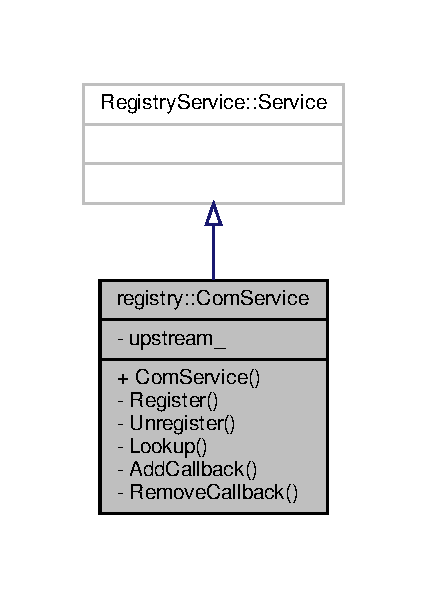
\includegraphics[width=205pt]{classregistry_1_1ComService__inherit__graph}
\end{center}
\end{figure}


Collaboration diagram for registry\+:\+:Com\+Service\+:\nopagebreak
\begin{figure}[H]
\begin{center}
\leavevmode
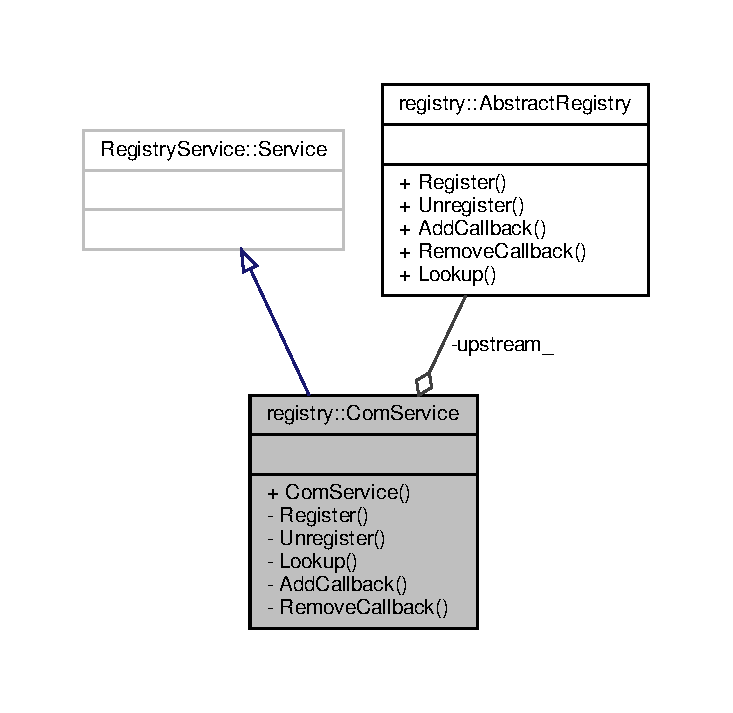
\includegraphics[width=350pt]{classregistry_1_1ComService__coll__graph}
\end{center}
\end{figure}
\subsection*{Public Member Functions}
\begin{DoxyCompactItemize}
\item 
\hyperlink{classregistry_1_1ComService_ac47bfa493c987731f6d7f6bc9a8adaf5}{Com\+Service} (\hyperlink{classregistry_1_1AbstractRegistry}{Abstract\+Registry} $\ast$ar)
\end{DoxyCompactItemize}
\subsection*{Private Member Functions}
\begin{DoxyCompactItemize}
\item 
grpc\+::\+Status \hyperlink{classregistry_1_1ComService_aae8b56b86316397140c4f1cc4824410a}{Register} (grpc\+::\+Server\+Context $\ast$cxt, Com\+Msg const $\ast$msg, Result $\ast$rslt) override
\item 
grpc\+::\+Status \hyperlink{classregistry_1_1ComService_a6a64c38b8adf4443f387af7ed786245c}{Unregister} (grpc\+::\+Server\+Context $\ast$cxt, Com\+Msg const $\ast$msg, Result $\ast$rslt) override
\item 
grpc\+::\+Status \hyperlink{classregistry_1_1ComService_a06ba4b402944f87dbce6c2ce37d8c279}{Lookup} (grpc\+::\+Server\+Context $\ast$cxt, Com\+Msg const $\ast$msg, Result $\ast$rslt) override
\item 
grpc\+::\+Status \hyperlink{classregistry_1_1ComService_aebee320ae37a1a8ea31792ba1e8e7ad6}{Add\+Callback} (grpc\+::\+Server\+Context $\ast$cxt, Com\+Msg const $\ast$msg, Result $\ast$rslt) override
\item 
grpc\+::\+Status \hyperlink{classregistry_1_1ComService_a702848d7aad6839ba216862478c00d25}{Remove\+Callback} (grpc\+::\+Server\+Context $\ast$cxt, Com\+Msg const $\ast$msg, Result $\ast$rslt) override
\end{DoxyCompactItemize}
\subsection*{Private Attributes}
\begin{DoxyCompactItemize}
\item 
\hyperlink{classregistry_1_1AbstractRegistry}{Abstract\+Registry} $\ast$ \hyperlink{classregistry_1_1ComService_a308106b15416761e61709d608f10d726}{upstream\+\_\+}
\begin{DoxyCompactList}\small\item\em An instance of Registry to be used to carry out the requested operations. \end{DoxyCompactList}\end{DoxyCompactItemize}


\subsection{Detailed Description}
g\+R\+PC service implementation. 

This classes directly uses the services of the Registry class to respond to R\+PC request. 

\subsection{Constructor \& Destructor Documentation}
\mbox{\Hypertarget{classregistry_1_1ComService_ac47bfa493c987731f6d7f6bc9a8adaf5}\label{classregistry_1_1ComService_ac47bfa493c987731f6d7f6bc9a8adaf5}} 
\index{registry\+::\+Com\+Service@{registry\+::\+Com\+Service}!Com\+Service@{Com\+Service}}
\index{Com\+Service@{Com\+Service}!registry\+::\+Com\+Service@{registry\+::\+Com\+Service}}
\subsubsection{\texorpdfstring{Com\+Service()}{ComService()}}
{\footnotesize\ttfamily registry\+::\+Com\+Service\+::\+Com\+Service (\begin{DoxyParamCaption}\item[{\hyperlink{classregistry_1_1AbstractRegistry}{Abstract\+Registry} $\ast$}]{ar }\end{DoxyParamCaption})\hspace{0.3cm}{\ttfamily [inline]}}



\subsection{Member Function Documentation}
\mbox{\Hypertarget{classregistry_1_1ComService_aebee320ae37a1a8ea31792ba1e8e7ad6}\label{classregistry_1_1ComService_aebee320ae37a1a8ea31792ba1e8e7ad6}} 
\index{registry\+::\+Com\+Service@{registry\+::\+Com\+Service}!Add\+Callback@{Add\+Callback}}
\index{Add\+Callback@{Add\+Callback}!registry\+::\+Com\+Service@{registry\+::\+Com\+Service}}
\subsubsection{\texorpdfstring{Add\+Callback()}{AddCallback()}}
{\footnotesize\ttfamily grpc\+::\+Status registry\+::\+Com\+Service\+::\+Add\+Callback (\begin{DoxyParamCaption}\item[{grpc\+::\+Server\+Context $\ast$}]{cxt,  }\item[{Com\+Msg const $\ast$}]{msg,  }\item[{Result $\ast$}]{rslt }\end{DoxyParamCaption})\hspace{0.3cm}{\ttfamily [inline]}, {\ttfamily [override]}, {\ttfamily [private]}}

\mbox{\Hypertarget{classregistry_1_1ComService_a06ba4b402944f87dbce6c2ce37d8c279}\label{classregistry_1_1ComService_a06ba4b402944f87dbce6c2ce37d8c279}} 
\index{registry\+::\+Com\+Service@{registry\+::\+Com\+Service}!Lookup@{Lookup}}
\index{Lookup@{Lookup}!registry\+::\+Com\+Service@{registry\+::\+Com\+Service}}
\subsubsection{\texorpdfstring{Lookup()}{Lookup()}}
{\footnotesize\ttfamily grpc\+::\+Status registry\+::\+Com\+Service\+::\+Lookup (\begin{DoxyParamCaption}\item[{grpc\+::\+Server\+Context $\ast$}]{cxt,  }\item[{Com\+Msg const $\ast$}]{msg,  }\item[{Result $\ast$}]{rslt }\end{DoxyParamCaption})\hspace{0.3cm}{\ttfamily [inline]}, {\ttfamily [override]}, {\ttfamily [private]}}

Here is the call graph for this function\+:\nopagebreak
\begin{figure}[H]
\begin{center}
\leavevmode
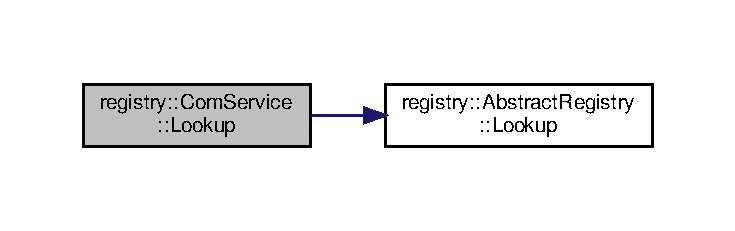
\includegraphics[width=350pt]{classregistry_1_1ComService_a06ba4b402944f87dbce6c2ce37d8c279_cgraph}
\end{center}
\end{figure}
\mbox{\Hypertarget{classregistry_1_1ComService_aae8b56b86316397140c4f1cc4824410a}\label{classregistry_1_1ComService_aae8b56b86316397140c4f1cc4824410a}} 
\index{registry\+::\+Com\+Service@{registry\+::\+Com\+Service}!Register@{Register}}
\index{Register@{Register}!registry\+::\+Com\+Service@{registry\+::\+Com\+Service}}
\subsubsection{\texorpdfstring{Register()}{Register()}}
{\footnotesize\ttfamily grpc\+::\+Status registry\+::\+Com\+Service\+::\+Register (\begin{DoxyParamCaption}\item[{grpc\+::\+Server\+Context $\ast$}]{cxt,  }\item[{Com\+Msg const $\ast$}]{msg,  }\item[{Result $\ast$}]{rslt }\end{DoxyParamCaption})\hspace{0.3cm}{\ttfamily [inline]}, {\ttfamily [override]}, {\ttfamily [private]}}

Here is the call graph for this function\+:\nopagebreak
\begin{figure}[H]
\begin{center}
\leavevmode
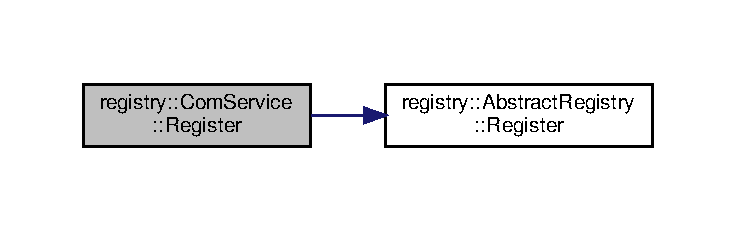
\includegraphics[width=350pt]{classregistry_1_1ComService_aae8b56b86316397140c4f1cc4824410a_cgraph}
\end{center}
\end{figure}
\mbox{\Hypertarget{classregistry_1_1ComService_a702848d7aad6839ba216862478c00d25}\label{classregistry_1_1ComService_a702848d7aad6839ba216862478c00d25}} 
\index{registry\+::\+Com\+Service@{registry\+::\+Com\+Service}!Remove\+Callback@{Remove\+Callback}}
\index{Remove\+Callback@{Remove\+Callback}!registry\+::\+Com\+Service@{registry\+::\+Com\+Service}}
\subsubsection{\texorpdfstring{Remove\+Callback()}{RemoveCallback()}}
{\footnotesize\ttfamily grpc\+::\+Status registry\+::\+Com\+Service\+::\+Remove\+Callback (\begin{DoxyParamCaption}\item[{grpc\+::\+Server\+Context $\ast$}]{cxt,  }\item[{Com\+Msg const $\ast$}]{msg,  }\item[{Result $\ast$}]{rslt }\end{DoxyParamCaption})\hspace{0.3cm}{\ttfamily [inline]}, {\ttfamily [override]}, {\ttfamily [private]}}

\mbox{\Hypertarget{classregistry_1_1ComService_a6a64c38b8adf4443f387af7ed786245c}\label{classregistry_1_1ComService_a6a64c38b8adf4443f387af7ed786245c}} 
\index{registry\+::\+Com\+Service@{registry\+::\+Com\+Service}!Unregister@{Unregister}}
\index{Unregister@{Unregister}!registry\+::\+Com\+Service@{registry\+::\+Com\+Service}}
\subsubsection{\texorpdfstring{Unregister()}{Unregister()}}
{\footnotesize\ttfamily grpc\+::\+Status registry\+::\+Com\+Service\+::\+Unregister (\begin{DoxyParamCaption}\item[{grpc\+::\+Server\+Context $\ast$}]{cxt,  }\item[{Com\+Msg const $\ast$}]{msg,  }\item[{Result $\ast$}]{rslt }\end{DoxyParamCaption})\hspace{0.3cm}{\ttfamily [inline]}, {\ttfamily [override]}, {\ttfamily [private]}}

Here is the call graph for this function\+:\nopagebreak
\begin{figure}[H]
\begin{center}
\leavevmode
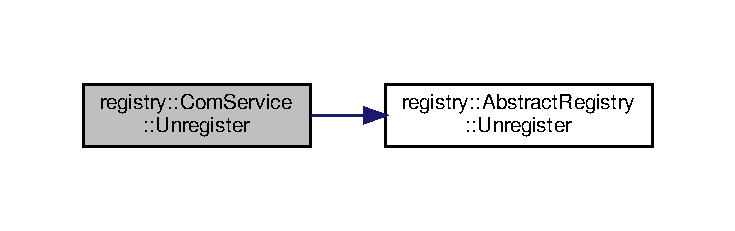
\includegraphics[width=350pt]{classregistry_1_1ComService_a6a64c38b8adf4443f387af7ed786245c_cgraph}
\end{center}
\end{figure}


\subsection{Member Data Documentation}
\mbox{\Hypertarget{classregistry_1_1ComService_a308106b15416761e61709d608f10d726}\label{classregistry_1_1ComService_a308106b15416761e61709d608f10d726}} 
\index{registry\+::\+Com\+Service@{registry\+::\+Com\+Service}!upstream\+\_\+@{upstream\+\_\+}}
\index{upstream\+\_\+@{upstream\+\_\+}!registry\+::\+Com\+Service@{registry\+::\+Com\+Service}}
\subsubsection{\texorpdfstring{upstream\+\_\+}{upstream\_}}
{\footnotesize\ttfamily \hyperlink{classregistry_1_1AbstractRegistry}{Abstract\+Registry}$\ast$ registry\+::\+Com\+Service\+::upstream\+\_\+\hspace{0.3cm}{\ttfamily [private]}}



An instance of Registry to be used to carry out the requested operations. 



The documentation for this class was generated from the following file\+:\begin{DoxyCompactItemize}
\item 
registry/src/\hyperlink{registry__core_8hpp}{registry\+\_\+core.\+hpp}\end{DoxyCompactItemize}

\hypertarget{structelem}{}\section{elem Struct Reference}
\label{structelem}\index{elem@{elem}}


{\ttfamily \#include $<$ring\+\_\+common.\+h$>$}



Collaboration diagram for elem\+:\nopagebreak
\begin{figure}[H]
\begin{center}
\leavevmode
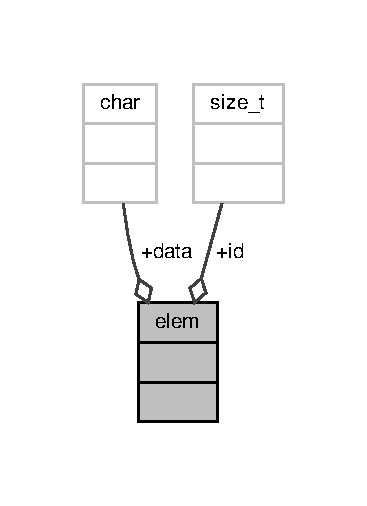
\includegraphics[width=176pt]{structelem__coll__graph}
\end{center}
\end{figure}
\subsection*{Public Attributes}
\begin{DoxyCompactItemize}
\item 
size\+\_\+t \hyperlink{structelem_a76c978bdb5b9645b0b2101b54b456d01}{id}
\item 
char \hyperlink{structelem_a135640bfc2ee968d1358592d8e9769e6}{data} \mbox{[}\hyperlink{ring__common_8h_a9036cd5ac8a8aa2ff3a4e4e00536f6d6}{k\+Elem\+Data\+Sz}\mbox{]}
\end{DoxyCompactItemize}


\subsection{Member Data Documentation}
\mbox{\Hypertarget{structelem_a135640bfc2ee968d1358592d8e9769e6}\label{structelem_a135640bfc2ee968d1358592d8e9769e6}} 
\index{elem@{elem}!data@{data}}
\index{data@{data}!elem@{elem}}
\subsubsection{\texorpdfstring{data}{data}}
{\footnotesize\ttfamily char elem\+::data\mbox{[}\hyperlink{ring__common_8h_a9036cd5ac8a8aa2ff3a4e4e00536f6d6}{k\+Elem\+Data\+Sz}\mbox{]}}

\mbox{\Hypertarget{structelem_a76c978bdb5b9645b0b2101b54b456d01}\label{structelem_a76c978bdb5b9645b0b2101b54b456d01}} 
\index{elem@{elem}!id@{id}}
\index{id@{id}!elem@{elem}}
\subsubsection{\texorpdfstring{id}{id}}
{\footnotesize\ttfamily size\+\_\+t elem\+::id}



The documentation for this struct was generated from the following file\+:\begin{DoxyCompactItemize}
\item 
ring/include/\hyperlink{ring__common_8h}{ring\+\_\+common.\+h}\end{DoxyCompactItemize}

\hypertarget{classExecFailed}{}\section{Exec\+Failed Class Reference}
\label{classExecFailed}\index{Exec\+Failed@{Exec\+Failed}}


{\ttfamily \#include $<$service\+\_\+manager.\+hpp$>$}



Inheritance diagram for Exec\+Failed\+:
\nopagebreak
\begin{figure}[H]
\begin{center}
\leavevmode
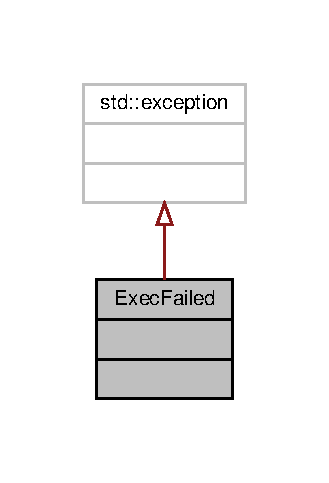
\includegraphics[width=158pt]{classExecFailed__inherit__graph}
\end{center}
\end{figure}


Collaboration diagram for Exec\+Failed\+:
\nopagebreak
\begin{figure}[H]
\begin{center}
\leavevmode
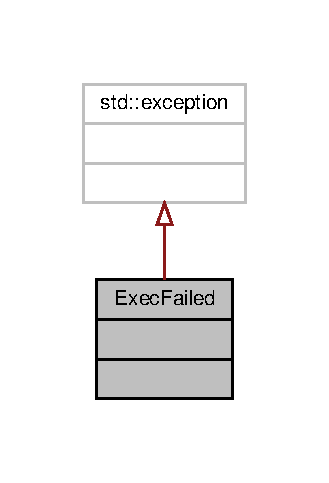
\includegraphics[width=158pt]{classExecFailed__coll__graph}
\end{center}
\end{figure}


The documentation for this class was generated from the following file\+:\begin{DoxyCompactItemize}
\item 
registry/src/\hyperlink{service__manager_8hpp}{service\+\_\+manager.\+hpp}\end{DoxyCompactItemize}

\hypertarget{classExtractor}{}\section{Extractor Class Reference}
\label{classExtractor}\index{Extractor@{Extractor}}


{\ttfamily \#include $<$extractor\+\_\+common.\+hpp$>$}



Collaboration diagram for Extractor\+:
\nopagebreak
\begin{figure}[H]
\begin{center}
\leavevmode
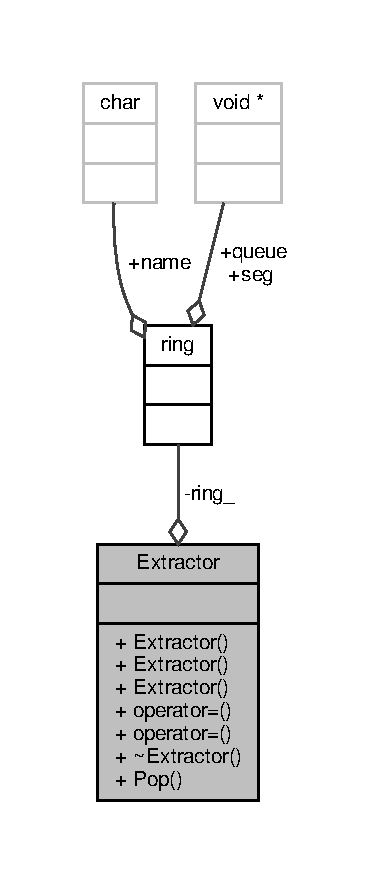
\includegraphics[width=179pt]{classExtractor__coll__graph}
\end{center}
\end{figure}
\subsection*{Public Member Functions}
\begin{DoxyCompactItemize}
\item 
\hyperlink{classExtractor_aaefc9c7f9b152b6380cb65c1e36ac95b}{Extractor} (std\+::string ownr\+\_\+name, std\+::string channel\+\_\+name, std\+::string addr=\char`\"{}127.\+0.\+0.\+1\char`\"{}, in\+\_\+port\+\_\+t port=40040)
\item 
\hyperlink{classExtractor_af0ccf57906e47cef731d7476956aca03}{Extractor} (\hyperlink{classExtractor}{Extractor} const \&)=delete
\item 
\hyperlink{classExtractor_ae3a09acb7a8e25f72b7cfc829f8aed8c}{Extractor} (\hyperlink{classExtractor}{Extractor} \&\&)=delete
\item 
\hyperlink{classExtractor}{Extractor} \& \hyperlink{classExtractor_abbc21689d5da9fb8115362a2e262e43f}{operator=} (\hyperlink{classExtractor}{Extractor} const \&)=delete
\item 
\hyperlink{classExtractor}{Extractor} \& \hyperlink{classExtractor_a4fae2fb922e5c5886c4a120aca43d877}{operator=} (\hyperlink{classExtractor}{Extractor} \&\&)=delete
\item 
\hyperlink{classExtractor_a0da249c590c92ed0714e8bd69ac236f4}{$\sim$\+Extractor} ()
\item 
\hyperlink{structelem}{elem} $\ast$ \hyperlink{classExtractor_a7632ce0dc24df1eeb659bb124e6b3031}{Pop} ()
\end{DoxyCompactItemize}
\subsection*{Private Attributes}
\begin{DoxyCompactItemize}
\item 
\hyperlink{structring}{ring} $\ast$ \hyperlink{classExtractor_a0e1370bcf808c900d1d3199350ebef41}{ring\+\_\+}
\end{DoxyCompactItemize}


\subsection{Detailed Description}
Used by client to lookup the registry information of any \hyperlink{classSpring}{Spring} we are interested in and then actually reading from their exposed ring buffers. 

\subsection{Constructor \& Destructor Documentation}
\mbox{\Hypertarget{classExtractor_aaefc9c7f9b152b6380cb65c1e36ac95b}\label{classExtractor_aaefc9c7f9b152b6380cb65c1e36ac95b}} 
\index{Extractor@{Extractor}!Extractor@{Extractor}}
\index{Extractor@{Extractor}!Extractor@{Extractor}}
\subsubsection{\texorpdfstring{Extractor()}{Extractor()}\hspace{0.1cm}{\footnotesize\ttfamily [1/3]}}
{\footnotesize\ttfamily Extractor\+::\+Extractor (\begin{DoxyParamCaption}\item[{std\+::string}]{ownr\+\_\+name,  }\item[{std\+::string}]{channel\+\_\+name,  }\item[{std\+::string}]{addr = {\ttfamily \char`\"{}127.0.0.1\char`\"{}},  }\item[{in\+\_\+port\+\_\+t}]{port = {\ttfamily 40040} }\end{DoxyParamCaption})}

Here is the call graph for this function\+:
\nopagebreak
\begin{figure}[H]
\begin{center}
\leavevmode
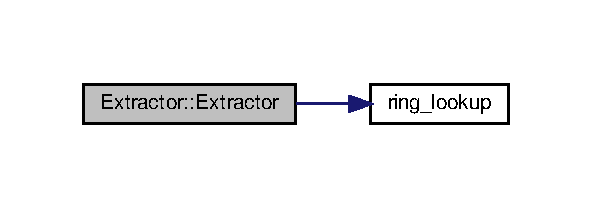
\includegraphics[width=284pt]{classExtractor_aaefc9c7f9b152b6380cb65c1e36ac95b_cgraph}
\end{center}
\end{figure}
\mbox{\Hypertarget{classExtractor_af0ccf57906e47cef731d7476956aca03}\label{classExtractor_af0ccf57906e47cef731d7476956aca03}} 
\index{Extractor@{Extractor}!Extractor@{Extractor}}
\index{Extractor@{Extractor}!Extractor@{Extractor}}
\subsubsection{\texorpdfstring{Extractor()}{Extractor()}\hspace{0.1cm}{\footnotesize\ttfamily [2/3]}}
{\footnotesize\ttfamily Extractor\+::\+Extractor (\begin{DoxyParamCaption}\item[{\hyperlink{classExtractor}{Extractor} const \&}]{ }\end{DoxyParamCaption})\hspace{0.3cm}{\ttfamily [delete]}}

\mbox{\Hypertarget{classExtractor_ae3a09acb7a8e25f72b7cfc829f8aed8c}\label{classExtractor_ae3a09acb7a8e25f72b7cfc829f8aed8c}} 
\index{Extractor@{Extractor}!Extractor@{Extractor}}
\index{Extractor@{Extractor}!Extractor@{Extractor}}
\subsubsection{\texorpdfstring{Extractor()}{Extractor()}\hspace{0.1cm}{\footnotesize\ttfamily [3/3]}}
{\footnotesize\ttfamily Extractor\+::\+Extractor (\begin{DoxyParamCaption}\item[{\hyperlink{classExtractor}{Extractor} \&\&}]{ }\end{DoxyParamCaption})\hspace{0.3cm}{\ttfamily [delete]}}

\mbox{\Hypertarget{classExtractor_a0da249c590c92ed0714e8bd69ac236f4}\label{classExtractor_a0da249c590c92ed0714e8bd69ac236f4}} 
\index{Extractor@{Extractor}!````~Extractor@{$\sim$\+Extractor}}
\index{````~Extractor@{$\sim$\+Extractor}!Extractor@{Extractor}}
\subsubsection{\texorpdfstring{$\sim$\+Extractor()}{~Extractor()}}
{\footnotesize\ttfamily Extractor\+::$\sim$\+Extractor (\begin{DoxyParamCaption}{ }\end{DoxyParamCaption})}



\subsection{Member Function Documentation}
\mbox{\Hypertarget{classExtractor_abbc21689d5da9fb8115362a2e262e43f}\label{classExtractor_abbc21689d5da9fb8115362a2e262e43f}} 
\index{Extractor@{Extractor}!operator=@{operator=}}
\index{operator=@{operator=}!Extractor@{Extractor}}
\subsubsection{\texorpdfstring{operator=()}{operator=()}\hspace{0.1cm}{\footnotesize\ttfamily [1/2]}}
{\footnotesize\ttfamily \hyperlink{classExtractor}{Extractor}\& Extractor\+::operator= (\begin{DoxyParamCaption}\item[{\hyperlink{classExtractor}{Extractor} const \&}]{ }\end{DoxyParamCaption})\hspace{0.3cm}{\ttfamily [delete]}}

\mbox{\Hypertarget{classExtractor_a4fae2fb922e5c5886c4a120aca43d877}\label{classExtractor_a4fae2fb922e5c5886c4a120aca43d877}} 
\index{Extractor@{Extractor}!operator=@{operator=}}
\index{operator=@{operator=}!Extractor@{Extractor}}
\subsubsection{\texorpdfstring{operator=()}{operator=()}\hspace{0.1cm}{\footnotesize\ttfamily [2/2]}}
{\footnotesize\ttfamily \hyperlink{classExtractor}{Extractor}\& Extractor\+::operator= (\begin{DoxyParamCaption}\item[{\hyperlink{classExtractor}{Extractor} \&\&}]{ }\end{DoxyParamCaption})\hspace{0.3cm}{\ttfamily [delete]}}

\mbox{\Hypertarget{classExtractor_a7632ce0dc24df1eeb659bb124e6b3031}\label{classExtractor_a7632ce0dc24df1eeb659bb124e6b3031}} 
\index{Extractor@{Extractor}!Pop@{Pop}}
\index{Pop@{Pop}!Extractor@{Extractor}}
\subsubsection{\texorpdfstring{Pop()}{Pop()}}
{\footnotesize\ttfamily \hyperlink{structelem}{elem} $\ast$ Extractor\+::\+Pop (\begin{DoxyParamCaption}{ }\end{DoxyParamCaption})}

Here is the call graph for this function\+:\nopagebreak
\begin{figure}[H]
\begin{center}
\leavevmode
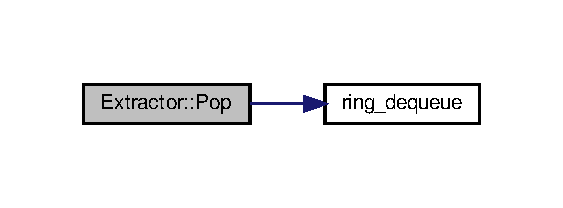
\includegraphics[width=270pt]{classExtractor_a7632ce0dc24df1eeb659bb124e6b3031_cgraph}
\end{center}
\end{figure}


\subsection{Member Data Documentation}
\mbox{\Hypertarget{classExtractor_a0e1370bcf808c900d1d3199350ebef41}\label{classExtractor_a0e1370bcf808c900d1d3199350ebef41}} 
\index{Extractor@{Extractor}!ring\+\_\+@{ring\+\_\+}}
\index{ring\+\_\+@{ring\+\_\+}!Extractor@{Extractor}}
\subsubsection{\texorpdfstring{ring\+\_\+}{ring\_}}
{\footnotesize\ttfamily \hyperlink{structring}{ring}$\ast$ Extractor\+::ring\+\_\+\hspace{0.3cm}{\ttfamily [private]}}

A multi-\/producer multi-\/consumer lockfree ring buffer that resides in a shared memory by all interested parties. This is unique for all Buffer\+Location instances that compare equal. 

The documentation for this class was generated from the following files\+:\begin{DoxyCompactItemize}
\item 
extractor/include/\hyperlink{extractor__common_8hpp}{extractor\+\_\+common.\+hpp}\item 
extractor/src/\hyperlink{extractor_8cpp}{extractor.\+cpp}\end{DoxyCompactItemize}

\hypertarget{classregistry_1_1ExtractorRegistryClient}{}\section{registry\+:\+:Extractor\+Registry\+Client Class Reference}
\label{classregistry_1_1ExtractorRegistryClient}\index{registry\+::\+Extractor\+Registry\+Client@{registry\+::\+Extractor\+Registry\+Client}}


{\ttfamily \#include $<$registry\+\_\+client.\+hpp$>$}



Collaboration diagram for registry\+:\+:Extractor\+Registry\+Client\+:\nopagebreak
\begin{figure}[H]
\begin{center}
\leavevmode
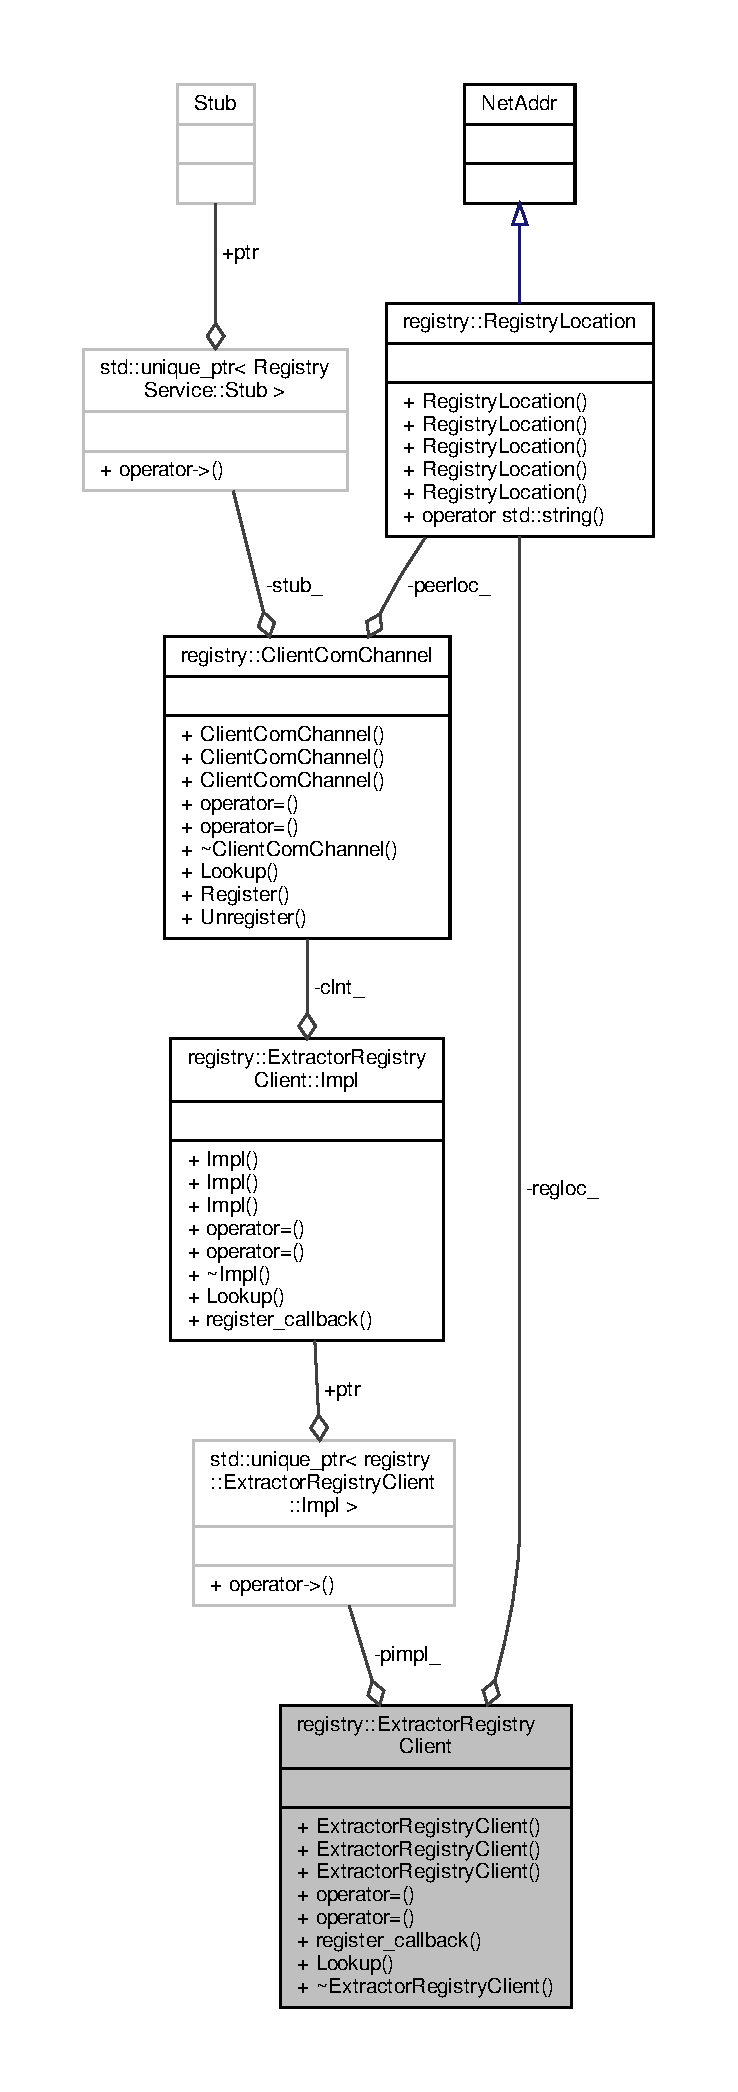
\includegraphics[height=550pt]{classregistry_1_1ExtractorRegistryClient__coll__graph}
\end{center}
\end{figure}
\subsection*{Classes}
\begin{DoxyCompactItemize}
\item 
class \hyperlink{classregistry_1_1ExtractorRegistryClient_1_1Impl}{Impl}
\end{DoxyCompactItemize}
\subsection*{Public Member Functions}
\begin{DoxyCompactItemize}
\item 
\hyperlink{classregistry_1_1ExtractorRegistryClient_a79e68c10ba8b6721529bf0b1f713f247}{Extractor\+Registry\+Client} (\hyperlink{structregistry_1_1RegistryLocation}{Registry\+Location} const \&) noexcept
\item 
\hyperlink{classregistry_1_1ExtractorRegistryClient_aace253a20f811a9252355809552f4b95}{Extractor\+Registry\+Client} (\hyperlink{classregistry_1_1ExtractorRegistryClient}{Extractor\+Registry\+Client} const \&)=delete
\item 
\hyperlink{classregistry_1_1ExtractorRegistryClient_a6f64a9ce2c92d5184b328720af9836a5}{Extractor\+Registry\+Client} (\hyperlink{classregistry_1_1ExtractorRegistryClient}{Extractor\+Registry\+Client} const \&\&)=delete
\item 
\hyperlink{classregistry_1_1ExtractorRegistryClient}{Extractor\+Registry\+Client} \& \hyperlink{classregistry_1_1ExtractorRegistryClient_ab84f0b91d01ae9dabe0318b771dc3bcf}{operator=} (\hyperlink{classregistry_1_1ExtractorRegistryClient}{Extractor\+Registry\+Client} const \&)=delete
\item 
\hyperlink{classregistry_1_1ExtractorRegistryClient}{Extractor\+Registry\+Client} \& \hyperlink{classregistry_1_1ExtractorRegistryClient_aafbb2652f8aa62f3c6e7dbbb4c72ab68}{operator=} (\hyperlink{classregistry_1_1ExtractorRegistryClient}{Extractor\+Registry\+Client} const \&\&)=delete
\item 
void \hyperlink{classregistry_1_1ExtractorRegistryClient_adc9670838114ce824bf7d79913aa5191}{register\+\_\+callback} (\hyperlink{classregistry_1_1Filter}{Filter}, std\+::function$<$ void()$>$)
\item 
std\+::vector$<$ \hyperlink{classregistry_1_1RegItem}{Reg\+Item} $>$ \hyperlink{classregistry_1_1ExtractorRegistryClient_aae214dba3e9dabd81844e6dfa3958eeb}{Lookup} (\hyperlink{classregistry_1_1Filter}{Filter} const \&) const
\item 
\hyperlink{classregistry_1_1ExtractorRegistryClient_a3c4ecec0c0a4ce7c25c7697889c253d9}{$\sim$\+Extractor\+Registry\+Client} () noexcept
\end{DoxyCompactItemize}
\subsection*{Private Attributes}
\begin{DoxyCompactItemize}
\item 
std\+::unique\+\_\+ptr$<$ \hyperlink{classregistry_1_1ExtractorRegistryClient_1_1Impl}{Impl} $>$ const \hyperlink{classregistry_1_1ExtractorRegistryClient_a7317fd7b55decd9a8f8c9db522db9b15}{pimpl\+\_\+}
\item 
\hyperlink{structregistry_1_1RegistryLocation}{Registry\+Location} const \hyperlink{classregistry_1_1ExtractorRegistryClient_a1092af361441aac2f5d84ae79267f4b7}{regloc\+\_\+}
\end{DoxyCompactItemize}


\subsection{Detailed Description}
This class is used by those that wnat to read the data items generated by other \hyperlink{classSpring}{Spring} parties. This class is used for communicating with a Registry as an \hyperlink{classExtractor}{Extractor}. It is not used read data items from other \hyperlink{classSpring}{Spring} instances. 

\subsection{Constructor \& Destructor Documentation}
\mbox{\Hypertarget{classregistry_1_1ExtractorRegistryClient_a79e68c10ba8b6721529bf0b1f713f247}\label{classregistry_1_1ExtractorRegistryClient_a79e68c10ba8b6721529bf0b1f713f247}} 
\index{registry\+::\+Extractor\+Registry\+Client@{registry\+::\+Extractor\+Registry\+Client}!Extractor\+Registry\+Client@{Extractor\+Registry\+Client}}
\index{Extractor\+Registry\+Client@{Extractor\+Registry\+Client}!registry\+::\+Extractor\+Registry\+Client@{registry\+::\+Extractor\+Registry\+Client}}
\subsubsection{\texorpdfstring{Extractor\+Registry\+Client()}{ExtractorRegistryClient()}\hspace{0.1cm}{\footnotesize\ttfamily [1/3]}}
{\footnotesize\ttfamily registry\+::\+Extractor\+Registry\+Client\+::\+Extractor\+Registry\+Client (\begin{DoxyParamCaption}\item[{\hyperlink{structregistry_1_1RegistryLocation}{Registry\+Location} const \&}]{loc }\end{DoxyParamCaption})\hspace{0.3cm}{\ttfamily [explicit]}, {\ttfamily [noexcept]}}

Here is the call graph for this function\+:\nopagebreak
\begin{figure}[H]
\begin{center}
\leavevmode
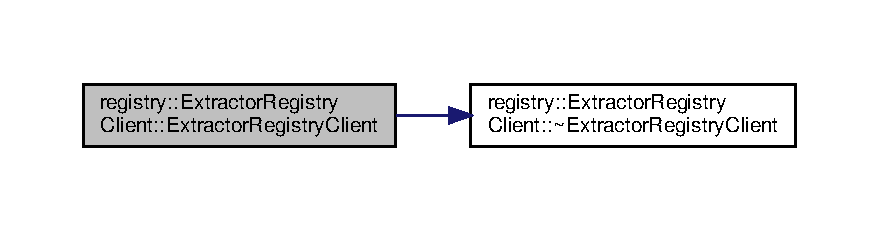
\includegraphics[width=350pt]{classregistry_1_1ExtractorRegistryClient_a79e68c10ba8b6721529bf0b1f713f247_cgraph}
\end{center}
\end{figure}
\mbox{\Hypertarget{classregistry_1_1ExtractorRegistryClient_aace253a20f811a9252355809552f4b95}\label{classregistry_1_1ExtractorRegistryClient_aace253a20f811a9252355809552f4b95}} 
\index{registry\+::\+Extractor\+Registry\+Client@{registry\+::\+Extractor\+Registry\+Client}!Extractor\+Registry\+Client@{Extractor\+Registry\+Client}}
\index{Extractor\+Registry\+Client@{Extractor\+Registry\+Client}!registry\+::\+Extractor\+Registry\+Client@{registry\+::\+Extractor\+Registry\+Client}}
\subsubsection{\texorpdfstring{Extractor\+Registry\+Client()}{ExtractorRegistryClient()}\hspace{0.1cm}{\footnotesize\ttfamily [2/3]}}
{\footnotesize\ttfamily registry\+::\+Extractor\+Registry\+Client\+::\+Extractor\+Registry\+Client (\begin{DoxyParamCaption}\item[{\hyperlink{classregistry_1_1ExtractorRegistryClient}{Extractor\+Registry\+Client} const \&}]{ }\end{DoxyParamCaption})\hspace{0.3cm}{\ttfamily [delete]}}

\mbox{\Hypertarget{classregistry_1_1ExtractorRegistryClient_a6f64a9ce2c92d5184b328720af9836a5}\label{classregistry_1_1ExtractorRegistryClient_a6f64a9ce2c92d5184b328720af9836a5}} 
\index{registry\+::\+Extractor\+Registry\+Client@{registry\+::\+Extractor\+Registry\+Client}!Extractor\+Registry\+Client@{Extractor\+Registry\+Client}}
\index{Extractor\+Registry\+Client@{Extractor\+Registry\+Client}!registry\+::\+Extractor\+Registry\+Client@{registry\+::\+Extractor\+Registry\+Client}}
\subsubsection{\texorpdfstring{Extractor\+Registry\+Client()}{ExtractorRegistryClient()}\hspace{0.1cm}{\footnotesize\ttfamily [3/3]}}
{\footnotesize\ttfamily registry\+::\+Extractor\+Registry\+Client\+::\+Extractor\+Registry\+Client (\begin{DoxyParamCaption}\item[{\hyperlink{classregistry_1_1ExtractorRegistryClient}{Extractor\+Registry\+Client} const \&\&}]{ }\end{DoxyParamCaption})\hspace{0.3cm}{\ttfamily [delete]}}

\mbox{\Hypertarget{classregistry_1_1ExtractorRegistryClient_a3c4ecec0c0a4ce7c25c7697889c253d9}\label{classregistry_1_1ExtractorRegistryClient_a3c4ecec0c0a4ce7c25c7697889c253d9}} 
\index{registry\+::\+Extractor\+Registry\+Client@{registry\+::\+Extractor\+Registry\+Client}!````~Extractor\+Registry\+Client@{$\sim$\+Extractor\+Registry\+Client}}
\index{````~Extractor\+Registry\+Client@{$\sim$\+Extractor\+Registry\+Client}!registry\+::\+Extractor\+Registry\+Client@{registry\+::\+Extractor\+Registry\+Client}}
\subsubsection{\texorpdfstring{$\sim$\+Extractor\+Registry\+Client()}{~ExtractorRegistryClient()}}
{\footnotesize\ttfamily registry\+::\+Extractor\+Registry\+Client\+::$\sim$\+Extractor\+Registry\+Client (\begin{DoxyParamCaption}{ }\end{DoxyParamCaption})\hspace{0.3cm}{\ttfamily [default]}, {\ttfamily [noexcept]}}

Here is the caller graph for this function\+:\nopagebreak
\begin{figure}[H]
\begin{center}
\leavevmode
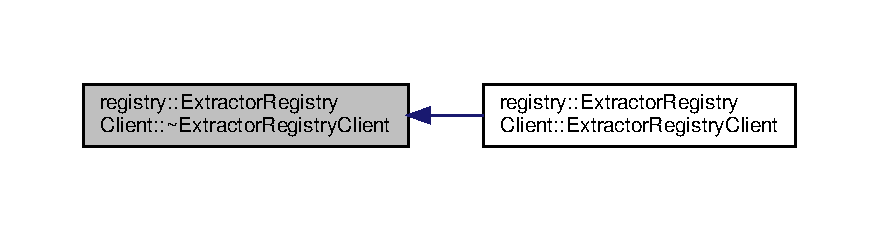
\includegraphics[width=350pt]{classregistry_1_1ExtractorRegistryClient_a3c4ecec0c0a4ce7c25c7697889c253d9_icgraph}
\end{center}
\end{figure}


\subsection{Member Function Documentation}
\mbox{\Hypertarget{classregistry_1_1ExtractorRegistryClient_aae214dba3e9dabd81844e6dfa3958eeb}\label{classregistry_1_1ExtractorRegistryClient_aae214dba3e9dabd81844e6dfa3958eeb}} 
\index{registry\+::\+Extractor\+Registry\+Client@{registry\+::\+Extractor\+Registry\+Client}!Lookup@{Lookup}}
\index{Lookup@{Lookup}!registry\+::\+Extractor\+Registry\+Client@{registry\+::\+Extractor\+Registry\+Client}}
\subsubsection{\texorpdfstring{Lookup()}{Lookup()}}
{\footnotesize\ttfamily std\+::vector$<$ \hyperlink{classregistry_1_1RegItem}{Reg\+Item} $>$ registry\+::\+Extractor\+Registry\+Client\+::\+Lookup (\begin{DoxyParamCaption}\item[{\hyperlink{classregistry_1_1Filter}{Filter} const \&}]{fltr }\end{DoxyParamCaption}) const}

\mbox{\Hypertarget{classregistry_1_1ExtractorRegistryClient_ab84f0b91d01ae9dabe0318b771dc3bcf}\label{classregistry_1_1ExtractorRegistryClient_ab84f0b91d01ae9dabe0318b771dc3bcf}} 
\index{registry\+::\+Extractor\+Registry\+Client@{registry\+::\+Extractor\+Registry\+Client}!operator=@{operator=}}
\index{operator=@{operator=}!registry\+::\+Extractor\+Registry\+Client@{registry\+::\+Extractor\+Registry\+Client}}
\subsubsection{\texorpdfstring{operator=()}{operator=()}\hspace{0.1cm}{\footnotesize\ttfamily [1/2]}}
{\footnotesize\ttfamily \hyperlink{classregistry_1_1ExtractorRegistryClient}{Extractor\+Registry\+Client}\& registry\+::\+Extractor\+Registry\+Client\+::operator= (\begin{DoxyParamCaption}\item[{\hyperlink{classregistry_1_1ExtractorRegistryClient}{Extractor\+Registry\+Client} const \&}]{ }\end{DoxyParamCaption})\hspace{0.3cm}{\ttfamily [delete]}}

\mbox{\Hypertarget{classregistry_1_1ExtractorRegistryClient_aafbb2652f8aa62f3c6e7dbbb4c72ab68}\label{classregistry_1_1ExtractorRegistryClient_aafbb2652f8aa62f3c6e7dbbb4c72ab68}} 
\index{registry\+::\+Extractor\+Registry\+Client@{registry\+::\+Extractor\+Registry\+Client}!operator=@{operator=}}
\index{operator=@{operator=}!registry\+::\+Extractor\+Registry\+Client@{registry\+::\+Extractor\+Registry\+Client}}
\subsubsection{\texorpdfstring{operator=()}{operator=()}\hspace{0.1cm}{\footnotesize\ttfamily [2/2]}}
{\footnotesize\ttfamily \hyperlink{classregistry_1_1ExtractorRegistryClient}{Extractor\+Registry\+Client}\& registry\+::\+Extractor\+Registry\+Client\+::operator= (\begin{DoxyParamCaption}\item[{\hyperlink{classregistry_1_1ExtractorRegistryClient}{Extractor\+Registry\+Client} const \&\&}]{ }\end{DoxyParamCaption})\hspace{0.3cm}{\ttfamily [delete]}}

\mbox{\Hypertarget{classregistry_1_1ExtractorRegistryClient_adc9670838114ce824bf7d79913aa5191}\label{classregistry_1_1ExtractorRegistryClient_adc9670838114ce824bf7d79913aa5191}} 
\index{registry\+::\+Extractor\+Registry\+Client@{registry\+::\+Extractor\+Registry\+Client}!register\+\_\+callback@{register\+\_\+callback}}
\index{register\+\_\+callback@{register\+\_\+callback}!registry\+::\+Extractor\+Registry\+Client@{registry\+::\+Extractor\+Registry\+Client}}
\subsubsection{\texorpdfstring{register\+\_\+callback()}{register\_callback()}}
{\footnotesize\ttfamily void registry\+::\+Extractor\+Registry\+Client\+::register\+\_\+callback (\begin{DoxyParamCaption}\item[{\hyperlink{classregistry_1_1Filter}{Filter}}]{flt,  }\item[{std\+::function$<$ void()$>$}]{cb }\end{DoxyParamCaption})}



\subsection{Member Data Documentation}
\mbox{\Hypertarget{classregistry_1_1ExtractorRegistryClient_a7317fd7b55decd9a8f8c9db522db9b15}\label{classregistry_1_1ExtractorRegistryClient_a7317fd7b55decd9a8f8c9db522db9b15}} 
\index{registry\+::\+Extractor\+Registry\+Client@{registry\+::\+Extractor\+Registry\+Client}!pimpl\+\_\+@{pimpl\+\_\+}}
\index{pimpl\+\_\+@{pimpl\+\_\+}!registry\+::\+Extractor\+Registry\+Client@{registry\+::\+Extractor\+Registry\+Client}}
\subsubsection{\texorpdfstring{pimpl\+\_\+}{pimpl\_}}
{\footnotesize\ttfamily std\+::unique\+\_\+ptr$<$\hyperlink{classregistry_1_1ExtractorRegistryClient_1_1Impl}{Impl}$>$ const registry\+::\+Extractor\+Registry\+Client\+::pimpl\+\_\+\hspace{0.3cm}{\ttfamily [private]}}

\mbox{\Hypertarget{classregistry_1_1ExtractorRegistryClient_a1092af361441aac2f5d84ae79267f4b7}\label{classregistry_1_1ExtractorRegistryClient_a1092af361441aac2f5d84ae79267f4b7}} 
\index{registry\+::\+Extractor\+Registry\+Client@{registry\+::\+Extractor\+Registry\+Client}!regloc\+\_\+@{regloc\+\_\+}}
\index{regloc\+\_\+@{regloc\+\_\+}!registry\+::\+Extractor\+Registry\+Client@{registry\+::\+Extractor\+Registry\+Client}}
\subsubsection{\texorpdfstring{regloc\+\_\+}{regloc\_}}
{\footnotesize\ttfamily \hyperlink{structregistry_1_1RegistryLocation}{Registry\+Location} const registry\+::\+Extractor\+Registry\+Client\+::regloc\+\_\+\hspace{0.3cm}{\ttfamily [private]}}

The location of the Registry that is used to lookup Reg\+Items to find the \hyperlink{classSpring}{Spring} we are interested in. 

The documentation for this class was generated from the following files\+:\begin{DoxyCompactItemize}
\item 
registry/include/\hyperlink{registry__client_8hpp}{registry\+\_\+client.\+hpp}\item 
registry/src/\hyperlink{registry__client__lib_8cpp}{registry\+\_\+client\+\_\+lib.\+cpp}\end{DoxyCompactItemize}

\hypertarget{classFakeChan}{}\section{Fake\+Chan Class Reference}
\label{classFakeChan}\index{Fake\+Chan@{Fake\+Chan}}


Collaboration diagram for Fake\+Chan\+:\nopagebreak
\begin{figure}[H]
\begin{center}
\leavevmode
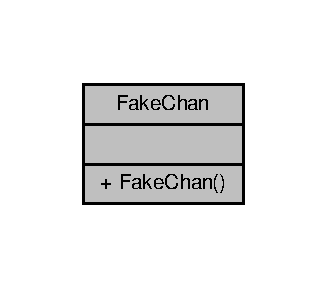
\includegraphics[width=157pt]{classFakeChan__coll__graph}
\end{center}
\end{figure}
\subsection*{Public Member Functions}
\begin{DoxyCompactItemize}
\item 
\hyperlink{classFakeChan_ad3563b881623aa552d98e78c24baef6c}{Fake\+Chan} () noexcept
\end{DoxyCompactItemize}


\subsection{Constructor \& Destructor Documentation}
\mbox{\Hypertarget{classFakeChan_ad3563b881623aa552d98e78c24baef6c}\label{classFakeChan_ad3563b881623aa552d98e78c24baef6c}} 
\index{Fake\+Chan@{Fake\+Chan}!Fake\+Chan@{Fake\+Chan}}
\index{Fake\+Chan@{Fake\+Chan}!Fake\+Chan@{Fake\+Chan}}
\subsubsection{\texorpdfstring{Fake\+Chan()}{FakeChan()}}
{\footnotesize\ttfamily Fake\+Chan\+::\+Fake\+Chan (\begin{DoxyParamCaption}{ }\end{DoxyParamCaption})\hspace{0.3cm}{\ttfamily [inline]}, {\ttfamily [noexcept]}}

Here is the call graph for this function\+:
\nopagebreak
\begin{figure}[H]
\begin{center}
\leavevmode
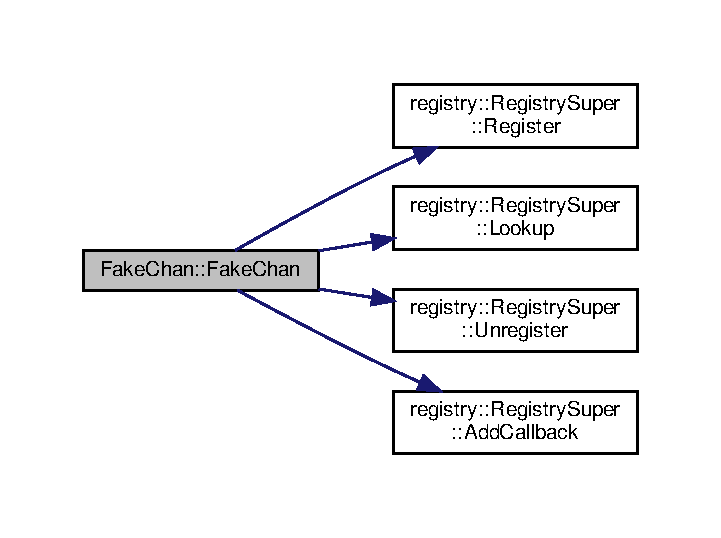
\includegraphics[width=346pt]{classFakeChan_ad3563b881623aa552d98e78c24baef6c_cgraph}
\end{center}
\end{figure}


The documentation for this class was generated from the following file\+:\begin{DoxyCompactItemize}
\item 
registry/test/\hyperlink{registry__core__tests_8cpp}{registry\+\_\+core\+\_\+tests.\+cpp}\end{DoxyCompactItemize}

\hypertarget{classregistry_1_1Filter}{}\section{registry\+:\+:Filter Class Reference}
\label{classregistry_1_1Filter}\index{registry\+::\+Filter@{registry\+::\+Filter}}


This class is used to search a Registry for Reg\+Items that match a specific pattern.  




{\ttfamily \#include $<$registry\+\_\+common.\+hpp$>$}



Collaboration diagram for registry\+:\+:Filter\+:\nopagebreak
\begin{figure}[H]
\begin{center}
\leavevmode
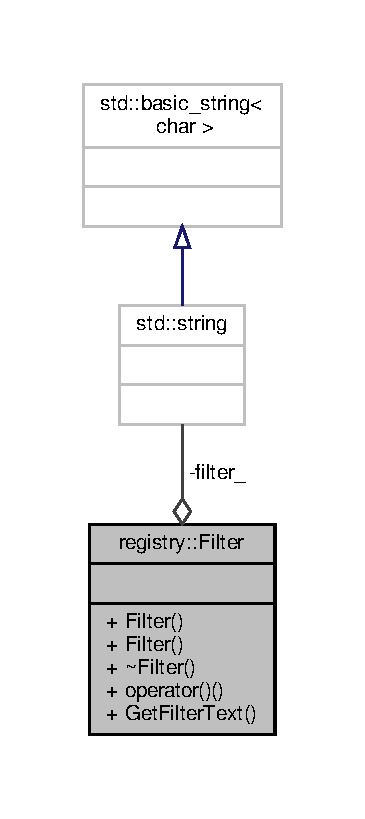
\includegraphics[width=175pt]{classregistry_1_1Filter__coll__graph}
\end{center}
\end{figure}
\subsection*{Public Member Functions}
\begin{DoxyCompactItemize}
\item 
\hyperlink{classregistry_1_1Filter_a91fa4858a3facd5ae4f302426ec0c126}{Filter} (\hyperlink{classregistry_1_1Filter_adca74845d8a5adb325dea6fb17dbcb2e}{Name\+Type} const \&filter\+\_\+text)
\item 
{\footnotesize template$<$typename T $>$ }\\\hyperlink{classregistry_1_1Filter_adb0037080036d7a808776054719bfb8c}{Filter} (T const \&fltr)
\item 
\hyperlink{classregistry_1_1Filter_a46e0bdb0721240eb83204817659bc1c0}{$\sim$\+Filter} () noexcept=default
\item 
bool \hyperlink{classregistry_1_1Filter_a88b3490d87c58983a16acb2c5fba077e}{operator()} (\hyperlink{classregistry_1_1Filter_adca74845d8a5adb325dea6fb17dbcb2e}{Name\+Type} const \&name) const
\item 
\hyperlink{classregistry_1_1Filter_adca74845d8a5adb325dea6fb17dbcb2e}{Name\+Type} const  \& \hyperlink{classregistry_1_1Filter_ac0f7882d01e05fe52a3d71b548aabd50}{Get\+Filter\+Text} () const
\end{DoxyCompactItemize}
\subsection*{Private Types}
\begin{DoxyCompactItemize}
\item 
using \hyperlink{classregistry_1_1Filter_adca74845d8a5adb325dea6fb17dbcb2e}{Name\+Type} = \hyperlink{structregistry_1_1BufferLocation_ad3c2279012b74798fa1e348507020fa4}{Buffer\+Location\+::\+Name\+Type}
\end{DoxyCompactItemize}
\subsection*{Private Attributes}
\begin{DoxyCompactItemize}
\item 
\hyperlink{structregistry_1_1BufferLocation_ad3c2279012b74798fa1e348507020fa4}{Buffer\+Location\+::\+Name\+Type} \hyperlink{classregistry_1_1Filter_a36d1de00325358200ebe9edadc92f14f}{filter\+\_\+}
\begin{DoxyCompactList}\small\item\em This is the specific pattern used to query a Registry. \end{DoxyCompactList}\end{DoxyCompactItemize}
\subsection*{Friends}
\begin{DoxyCompactItemize}
\item 
bool \hyperlink{classregistry_1_1Filter_a2258c07ccd7708c4f4cad83338a14c4d}{operator==} (\hyperlink{classregistry_1_1Filter}{Filter} const \&, \hyperlink{classregistry_1_1Filter}{Filter} const \&)
\end{DoxyCompactItemize}


\subsection{Detailed Description}
This class is used to search a Registry for Reg\+Items that match a specific pattern. 

\subsection{Member Typedef Documentation}
\mbox{\Hypertarget{classregistry_1_1Filter_adca74845d8a5adb325dea6fb17dbcb2e}\label{classregistry_1_1Filter_adca74845d8a5adb325dea6fb17dbcb2e}} 
\index{registry\+::\+Filter@{registry\+::\+Filter}!Name\+Type@{Name\+Type}}
\index{Name\+Type@{Name\+Type}!registry\+::\+Filter@{registry\+::\+Filter}}
\subsubsection{\texorpdfstring{Name\+Type}{NameType}}
{\footnotesize\ttfamily using \hyperlink{classregistry_1_1Filter_adca74845d8a5adb325dea6fb17dbcb2e}{registry\+::\+Filter\+::\+Name\+Type} =  \hyperlink{structregistry_1_1BufferLocation_ad3c2279012b74798fa1e348507020fa4}{Buffer\+Location\+::\+Name\+Type}\hspace{0.3cm}{\ttfamily [private]}}



\subsection{Constructor \& Destructor Documentation}
\mbox{\Hypertarget{classregistry_1_1Filter_a91fa4858a3facd5ae4f302426ec0c126}\label{classregistry_1_1Filter_a91fa4858a3facd5ae4f302426ec0c126}} 
\index{registry\+::\+Filter@{registry\+::\+Filter}!Filter@{Filter}}
\index{Filter@{Filter}!registry\+::\+Filter@{registry\+::\+Filter}}
\subsubsection{\texorpdfstring{Filter()}{Filter()}\hspace{0.1cm}{\footnotesize\ttfamily [1/2]}}
{\footnotesize\ttfamily registry\+::\+Filter\+::\+Filter (\begin{DoxyParamCaption}\item[{\hyperlink{classregistry_1_1Filter_adca74845d8a5adb325dea6fb17dbcb2e}{Name\+Type} const \&}]{filter\+\_\+text }\end{DoxyParamCaption})\hspace{0.3cm}{\ttfamily [inline]}}

\mbox{\Hypertarget{classregistry_1_1Filter_adb0037080036d7a808776054719bfb8c}\label{classregistry_1_1Filter_adb0037080036d7a808776054719bfb8c}} 
\index{registry\+::\+Filter@{registry\+::\+Filter}!Filter@{Filter}}
\index{Filter@{Filter}!registry\+::\+Filter@{registry\+::\+Filter}}
\subsubsection{\texorpdfstring{Filter()}{Filter()}\hspace{0.1cm}{\footnotesize\ttfamily [2/2]}}
{\footnotesize\ttfamily template$<$typename T $>$ \\
registry\+::\+Filter\+::\+Filter (\begin{DoxyParamCaption}\item[{T const \&}]{fltr }\end{DoxyParamCaption})\hspace{0.3cm}{\ttfamily [inline]}, {\ttfamily [explicit]}}

\mbox{\Hypertarget{classregistry_1_1Filter_a46e0bdb0721240eb83204817659bc1c0}\label{classregistry_1_1Filter_a46e0bdb0721240eb83204817659bc1c0}} 
\index{registry\+::\+Filter@{registry\+::\+Filter}!````~Filter@{$\sim$\+Filter}}
\index{````~Filter@{$\sim$\+Filter}!registry\+::\+Filter@{registry\+::\+Filter}}
\subsubsection{\texorpdfstring{$\sim$\+Filter()}{~Filter()}}
{\footnotesize\ttfamily registry\+::\+Filter\+::$\sim$\+Filter (\begin{DoxyParamCaption}{ }\end{DoxyParamCaption})\hspace{0.3cm}{\ttfamily [default]}, {\ttfamily [noexcept]}}



\subsection{Member Function Documentation}
\mbox{\Hypertarget{classregistry_1_1Filter_ac0f7882d01e05fe52a3d71b548aabd50}\label{classregistry_1_1Filter_ac0f7882d01e05fe52a3d71b548aabd50}} 
\index{registry\+::\+Filter@{registry\+::\+Filter}!Get\+Filter\+Text@{Get\+Filter\+Text}}
\index{Get\+Filter\+Text@{Get\+Filter\+Text}!registry\+::\+Filter@{registry\+::\+Filter}}
\subsubsection{\texorpdfstring{Get\+Filter\+Text()}{GetFilterText()}}
{\footnotesize\ttfamily \hyperlink{classregistry_1_1Filter_adca74845d8a5adb325dea6fb17dbcb2e}{Name\+Type} const\& registry\+::\+Filter\+::\+Get\+Filter\+Text (\begin{DoxyParamCaption}{ }\end{DoxyParamCaption}) const\hspace{0.3cm}{\ttfamily [inline]}}

Here is the caller graph for this function\+:
\nopagebreak
\begin{figure}[H]
\begin{center}
\leavevmode
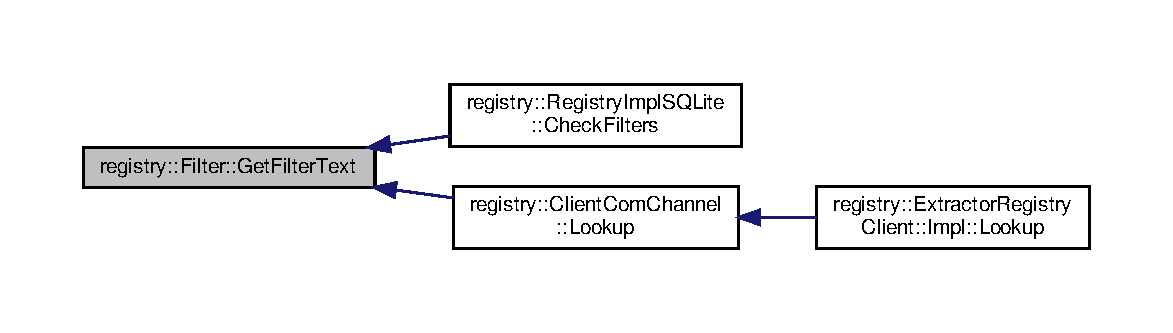
\includegraphics[width=350pt]{classregistry_1_1Filter_ac0f7882d01e05fe52a3d71b548aabd50_icgraph}
\end{center}
\end{figure}
\mbox{\Hypertarget{classregistry_1_1Filter_a88b3490d87c58983a16acb2c5fba077e}\label{classregistry_1_1Filter_a88b3490d87c58983a16acb2c5fba077e}} 
\index{registry\+::\+Filter@{registry\+::\+Filter}!operator()@{operator()}}
\index{operator()@{operator()}!registry\+::\+Filter@{registry\+::\+Filter}}
\subsubsection{\texorpdfstring{operator()()}{operator()()}}
{\footnotesize\ttfamily bool registry\+::\+Filter\+::operator() (\begin{DoxyParamCaption}\item[{\hyperlink{classregistry_1_1Filter_adca74845d8a5adb325dea6fb17dbcb2e}{Name\+Type} const \&}]{name }\end{DoxyParamCaption}) const\hspace{0.3cm}{\ttfamily [inline]}}

Here is the call graph for this function\+:
\nopagebreak
\begin{figure}[H]
\begin{center}
\leavevmode
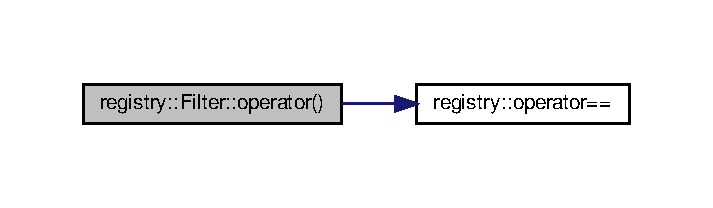
\includegraphics[width=342pt]{classregistry_1_1Filter_a88b3490d87c58983a16acb2c5fba077e_cgraph}
\end{center}
\end{figure}


\subsection{Friends And Related Function Documentation}
\mbox{\Hypertarget{classregistry_1_1Filter_a2258c07ccd7708c4f4cad83338a14c4d}\label{classregistry_1_1Filter_a2258c07ccd7708c4f4cad83338a14c4d}} 
\index{registry\+::\+Filter@{registry\+::\+Filter}!operator==@{operator==}}
\index{operator==@{operator==}!registry\+::\+Filter@{registry\+::\+Filter}}
\subsubsection{\texorpdfstring{operator==}{operator==}}
{\footnotesize\ttfamily bool operator== (\begin{DoxyParamCaption}\item[{\hyperlink{classregistry_1_1Filter}{Filter} const \&}]{f1,  }\item[{\hyperlink{classregistry_1_1Filter}{Filter} const \&}]{f2 }\end{DoxyParamCaption})\hspace{0.3cm}{\ttfamily [friend]}}



\subsection{Member Data Documentation}
\mbox{\Hypertarget{classregistry_1_1Filter_a36d1de00325358200ebe9edadc92f14f}\label{classregistry_1_1Filter_a36d1de00325358200ebe9edadc92f14f}} 
\index{registry\+::\+Filter@{registry\+::\+Filter}!filter\+\_\+@{filter\+\_\+}}
\index{filter\+\_\+@{filter\+\_\+}!registry\+::\+Filter@{registry\+::\+Filter}}
\subsubsection{\texorpdfstring{filter\+\_\+}{filter\_}}
{\footnotesize\ttfamily \hyperlink{structregistry_1_1BufferLocation_ad3c2279012b74798fa1e348507020fa4}{Buffer\+Location\+::\+Name\+Type} registry\+::\+Filter\+::filter\+\_\+\hspace{0.3cm}{\ttfamily [private]}}



This is the specific pattern used to query a Registry. 



The documentation for this class was generated from the following file\+:\begin{DoxyCompactItemize}
\item 
registry/include/\hyperlink{registry__common_8hpp}{registry\+\_\+common.\+hpp}\end{DoxyCompactItemize}

\hypertarget{classForkFailed}{}\section{Fork\+Failed Class Reference}
\label{classForkFailed}\index{Fork\+Failed@{Fork\+Failed}}


{\ttfamily \#include $<$service\+\_\+manager.\+hpp$>$}



Inheritance diagram for Fork\+Failed\+:
\nopagebreak
\begin{figure}[H]
\begin{center}
\leavevmode
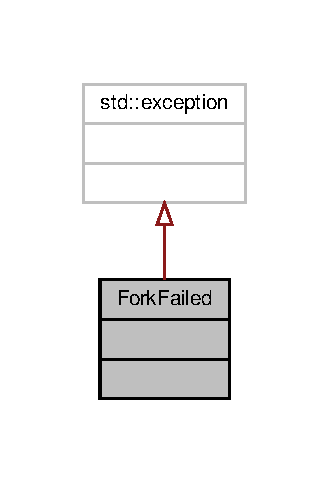
\includegraphics[width=158pt]{classForkFailed__inherit__graph}
\end{center}
\end{figure}


Collaboration diagram for Fork\+Failed\+:
\nopagebreak
\begin{figure}[H]
\begin{center}
\leavevmode
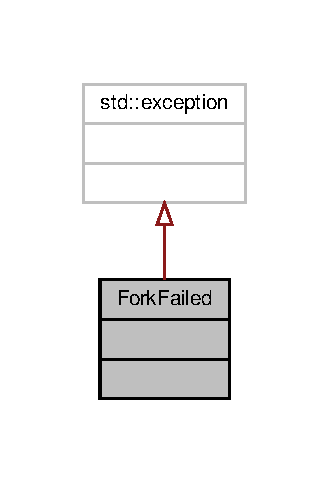
\includegraphics[width=158pt]{classForkFailed__coll__graph}
\end{center}
\end{figure}


The documentation for this class was generated from the following file\+:\begin{DoxyCompactItemize}
\item 
registry/src/\hyperlink{service__manager_8hpp}{service\+\_\+manager.\+hpp}\end{DoxyCompactItemize}

\hypertarget{classregistry_1_1SpringRegistryClient_1_1Impl}{}\section{registry\+:\+:Spring\+Registry\+Client\+:\+:Impl Class Reference}
\label{classregistry_1_1SpringRegistryClient_1_1Impl}\index{registry\+::\+Spring\+Registry\+Client\+::\+Impl@{registry\+::\+Spring\+Registry\+Client\+::\+Impl}}


Collaboration diagram for registry\+:\+:Spring\+Registry\+Client\+:\+:Impl\+:\nopagebreak
\begin{figure}[H]
\begin{center}
\leavevmode
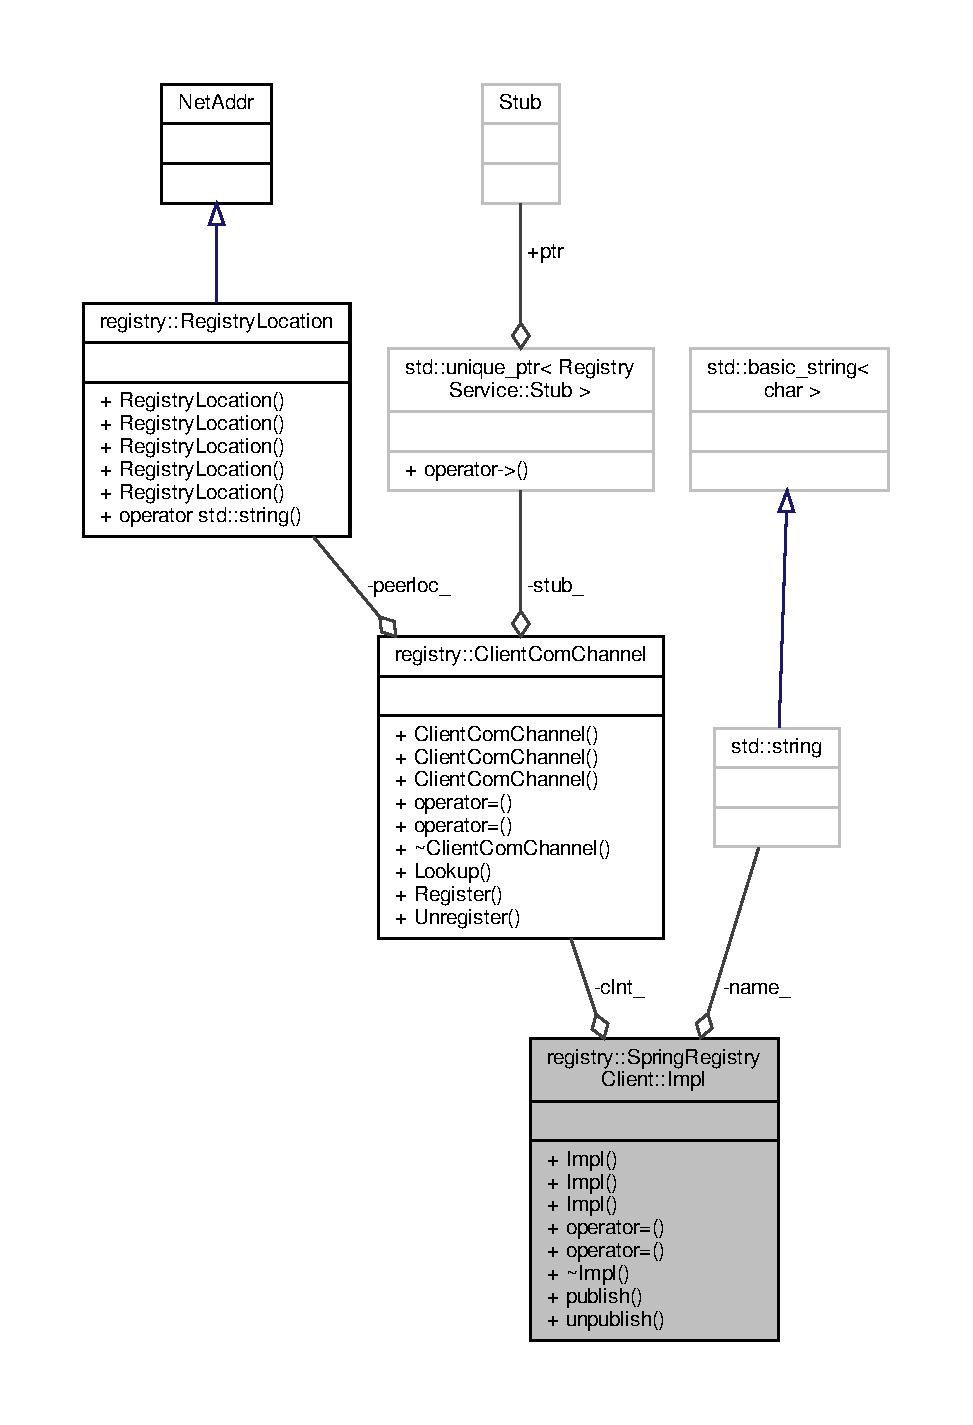
\includegraphics[width=350pt]{classregistry_1_1SpringRegistryClient_1_1Impl__coll__graph}
\end{center}
\end{figure}
\subsection*{Public Member Functions}
\begin{DoxyCompactItemize}
\item 
\hyperlink{classregistry_1_1SpringRegistryClient_1_1Impl_a5c16208aad64fd576de9b37cb0d2ce7d}{Impl} (std\+::string const \&n, \hyperlink{structregistry_1_1RegistryLocation}{Registry\+Location} const \&l)
\item 
\hyperlink{classregistry_1_1SpringRegistryClient_1_1Impl_aeb96c2a4edeedf35e6a68bfc04d296d5}{Impl} (\hyperlink{classregistry_1_1SpringRegistryClient_1_1Impl}{Impl} const \&)=delete
\item 
\hyperlink{classregistry_1_1SpringRegistryClient_1_1Impl_aa2ff8d87af51138e71cf20e5f7f05118}{Impl} (\hyperlink{classregistry_1_1SpringRegistryClient_1_1Impl}{Impl} \&\&)=delete
\item 
\hyperlink{classregistry_1_1SpringRegistryClient_1_1Impl}{Impl} \& \hyperlink{classregistry_1_1SpringRegistryClient_1_1Impl_a2a52cac36cd703b782fb2feea1ee55fc}{operator=} (\hyperlink{classregistry_1_1SpringRegistryClient_1_1Impl}{Impl} const \&)=delete
\item 
\hyperlink{classregistry_1_1SpringRegistryClient_1_1Impl}{Impl} \& \hyperlink{classregistry_1_1SpringRegistryClient_1_1Impl_af30a878a4cc61b28f6b9d3e429be79fc}{operator=} (\hyperlink{classregistry_1_1SpringRegistryClient_1_1Impl}{Impl} \&\&)=delete
\item 
\hyperlink{classregistry_1_1SpringRegistryClient_1_1Impl_aaf37891f1445665c32a7c331e7343d67}{$\sim$\+Impl} () noexcept=default
\item 
void \hyperlink{classregistry_1_1SpringRegistryClient_1_1Impl_a1b7694f4de9c0f95fe4ff76c54618057}{publish} (\hyperlink{structregistry_1_1BufferLocation}{Buffer\+Location} const \&location) const
\item 
void \hyperlink{classregistry_1_1SpringRegistryClient_1_1Impl_ac3b721317dfb893e191d3d112575a627}{unpublish} (\hyperlink{structregistry_1_1BufferLocation}{Buffer\+Location} const \&name) const
\end{DoxyCompactItemize}
\subsection*{Private Attributes}
\begin{DoxyCompactItemize}
\item 
std\+::string const \hyperlink{classregistry_1_1SpringRegistryClient_1_1Impl_ad1c90e7182c68d7d48702d8b8329e805}{name\+\_\+}
\item 
\hyperlink{classregistry_1_1ClientComChannel}{Client\+Com\+Channel} const \hyperlink{classregistry_1_1SpringRegistryClient_1_1Impl_ab0b715b0d49462786aa052d732f8207c}{clnt\+\_\+}
\end{DoxyCompactItemize}


\subsection{Constructor \& Destructor Documentation}
\mbox{\Hypertarget{classregistry_1_1SpringRegistryClient_1_1Impl_a5c16208aad64fd576de9b37cb0d2ce7d}\label{classregistry_1_1SpringRegistryClient_1_1Impl_a5c16208aad64fd576de9b37cb0d2ce7d}} 
\index{registry\+::\+Spring\+Registry\+Client\+::\+Impl@{registry\+::\+Spring\+Registry\+Client\+::\+Impl}!Impl@{Impl}}
\index{Impl@{Impl}!registry\+::\+Spring\+Registry\+Client\+::\+Impl@{registry\+::\+Spring\+Registry\+Client\+::\+Impl}}
\subsubsection{\texorpdfstring{Impl()}{Impl()}\hspace{0.1cm}{\footnotesize\ttfamily [1/3]}}
{\footnotesize\ttfamily registry\+::\+Spring\+Registry\+Client\+::\+Impl\+::\+Impl (\begin{DoxyParamCaption}\item[{std\+::string const \&}]{n,  }\item[{\hyperlink{structregistry_1_1RegistryLocation}{Registry\+Location} const \&}]{l }\end{DoxyParamCaption})}

\mbox{\Hypertarget{classregistry_1_1SpringRegistryClient_1_1Impl_aeb96c2a4edeedf35e6a68bfc04d296d5}\label{classregistry_1_1SpringRegistryClient_1_1Impl_aeb96c2a4edeedf35e6a68bfc04d296d5}} 
\index{registry\+::\+Spring\+Registry\+Client\+::\+Impl@{registry\+::\+Spring\+Registry\+Client\+::\+Impl}!Impl@{Impl}}
\index{Impl@{Impl}!registry\+::\+Spring\+Registry\+Client\+::\+Impl@{registry\+::\+Spring\+Registry\+Client\+::\+Impl}}
\subsubsection{\texorpdfstring{Impl()}{Impl()}\hspace{0.1cm}{\footnotesize\ttfamily [2/3]}}
{\footnotesize\ttfamily registry\+::\+Spring\+Registry\+Client\+::\+Impl\+::\+Impl (\begin{DoxyParamCaption}\item[{\hyperlink{classregistry_1_1SpringRegistryClient_1_1Impl}{Impl} const \&}]{ }\end{DoxyParamCaption})\hspace{0.3cm}{\ttfamily [delete]}}

\mbox{\Hypertarget{classregistry_1_1SpringRegistryClient_1_1Impl_aa2ff8d87af51138e71cf20e5f7f05118}\label{classregistry_1_1SpringRegistryClient_1_1Impl_aa2ff8d87af51138e71cf20e5f7f05118}} 
\index{registry\+::\+Spring\+Registry\+Client\+::\+Impl@{registry\+::\+Spring\+Registry\+Client\+::\+Impl}!Impl@{Impl}}
\index{Impl@{Impl}!registry\+::\+Spring\+Registry\+Client\+::\+Impl@{registry\+::\+Spring\+Registry\+Client\+::\+Impl}}
\subsubsection{\texorpdfstring{Impl()}{Impl()}\hspace{0.1cm}{\footnotesize\ttfamily [3/3]}}
{\footnotesize\ttfamily registry\+::\+Spring\+Registry\+Client\+::\+Impl\+::\+Impl (\begin{DoxyParamCaption}\item[{\hyperlink{classregistry_1_1SpringRegistryClient_1_1Impl}{Impl} \&\&}]{ }\end{DoxyParamCaption})\hspace{0.3cm}{\ttfamily [delete]}}

\mbox{\Hypertarget{classregistry_1_1SpringRegistryClient_1_1Impl_aaf37891f1445665c32a7c331e7343d67}\label{classregistry_1_1SpringRegistryClient_1_1Impl_aaf37891f1445665c32a7c331e7343d67}} 
\index{registry\+::\+Spring\+Registry\+Client\+::\+Impl@{registry\+::\+Spring\+Registry\+Client\+::\+Impl}!````~Impl@{$\sim$\+Impl}}
\index{````~Impl@{$\sim$\+Impl}!registry\+::\+Spring\+Registry\+Client\+::\+Impl@{registry\+::\+Spring\+Registry\+Client\+::\+Impl}}
\subsubsection{\texorpdfstring{$\sim$\+Impl()}{~Impl()}}
{\footnotesize\ttfamily registry\+::\+Spring\+Registry\+Client\+::\+Impl\+::$\sim$\+Impl (\begin{DoxyParamCaption}{ }\end{DoxyParamCaption})\hspace{0.3cm}{\ttfamily [default]}, {\ttfamily [noexcept]}}



\subsection{Member Function Documentation}
\mbox{\Hypertarget{classregistry_1_1SpringRegistryClient_1_1Impl_a2a52cac36cd703b782fb2feea1ee55fc}\label{classregistry_1_1SpringRegistryClient_1_1Impl_a2a52cac36cd703b782fb2feea1ee55fc}} 
\index{registry\+::\+Spring\+Registry\+Client\+::\+Impl@{registry\+::\+Spring\+Registry\+Client\+::\+Impl}!operator=@{operator=}}
\index{operator=@{operator=}!registry\+::\+Spring\+Registry\+Client\+::\+Impl@{registry\+::\+Spring\+Registry\+Client\+::\+Impl}}
\subsubsection{\texorpdfstring{operator=()}{operator=()}\hspace{0.1cm}{\footnotesize\ttfamily [1/2]}}
{\footnotesize\ttfamily \hyperlink{classregistry_1_1SpringRegistryClient_1_1Impl}{Impl}\& registry\+::\+Spring\+Registry\+Client\+::\+Impl\+::operator= (\begin{DoxyParamCaption}\item[{\hyperlink{classregistry_1_1SpringRegistryClient_1_1Impl}{Impl} const \&}]{ }\end{DoxyParamCaption})\hspace{0.3cm}{\ttfamily [delete]}}

\mbox{\Hypertarget{classregistry_1_1SpringRegistryClient_1_1Impl_af30a878a4cc61b28f6b9d3e429be79fc}\label{classregistry_1_1SpringRegistryClient_1_1Impl_af30a878a4cc61b28f6b9d3e429be79fc}} 
\index{registry\+::\+Spring\+Registry\+Client\+::\+Impl@{registry\+::\+Spring\+Registry\+Client\+::\+Impl}!operator=@{operator=}}
\index{operator=@{operator=}!registry\+::\+Spring\+Registry\+Client\+::\+Impl@{registry\+::\+Spring\+Registry\+Client\+::\+Impl}}
\subsubsection{\texorpdfstring{operator=()}{operator=()}\hspace{0.1cm}{\footnotesize\ttfamily [2/2]}}
{\footnotesize\ttfamily \hyperlink{classregistry_1_1SpringRegistryClient_1_1Impl}{Impl}\& registry\+::\+Spring\+Registry\+Client\+::\+Impl\+::operator= (\begin{DoxyParamCaption}\item[{\hyperlink{classregistry_1_1SpringRegistryClient_1_1Impl}{Impl} \&\&}]{ }\end{DoxyParamCaption})\hspace{0.3cm}{\ttfamily [delete]}}

\mbox{\Hypertarget{classregistry_1_1SpringRegistryClient_1_1Impl_a1b7694f4de9c0f95fe4ff76c54618057}\label{classregistry_1_1SpringRegistryClient_1_1Impl_a1b7694f4de9c0f95fe4ff76c54618057}} 
\index{registry\+::\+Spring\+Registry\+Client\+::\+Impl@{registry\+::\+Spring\+Registry\+Client\+::\+Impl}!publish@{publish}}
\index{publish@{publish}!registry\+::\+Spring\+Registry\+Client\+::\+Impl@{registry\+::\+Spring\+Registry\+Client\+::\+Impl}}
\subsubsection{\texorpdfstring{publish()}{publish()}}
{\footnotesize\ttfamily void registry\+::\+Spring\+Registry\+Client\+::\+Impl\+::publish (\begin{DoxyParamCaption}\item[{\hyperlink{structregistry_1_1BufferLocation}{Buffer\+Location} const \&}]{location }\end{DoxyParamCaption}) const}

Here is the call graph for this function\+:
\nopagebreak
\begin{figure}[H]
\begin{center}
\leavevmode
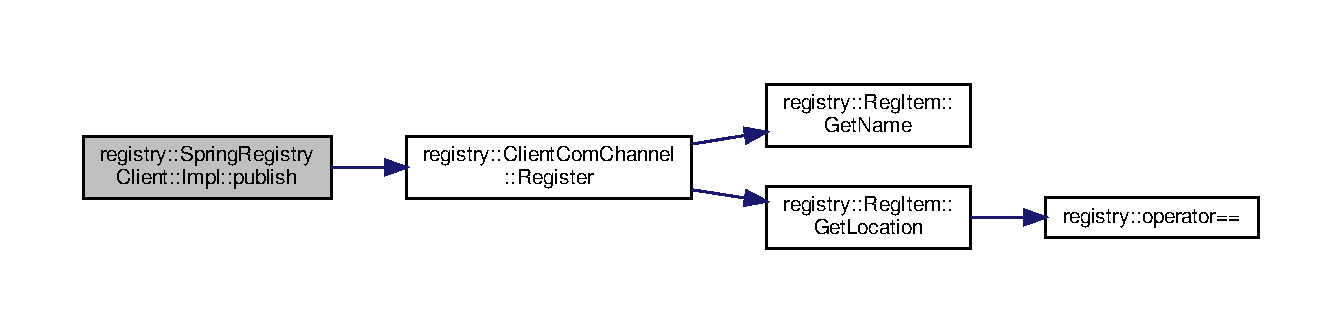
\includegraphics[width=350pt]{classregistry_1_1SpringRegistryClient_1_1Impl_a1b7694f4de9c0f95fe4ff76c54618057_cgraph}
\end{center}
\end{figure}
\mbox{\Hypertarget{classregistry_1_1SpringRegistryClient_1_1Impl_ac3b721317dfb893e191d3d112575a627}\label{classregistry_1_1SpringRegistryClient_1_1Impl_ac3b721317dfb893e191d3d112575a627}} 
\index{registry\+::\+Spring\+Registry\+Client\+::\+Impl@{registry\+::\+Spring\+Registry\+Client\+::\+Impl}!unpublish@{unpublish}}
\index{unpublish@{unpublish}!registry\+::\+Spring\+Registry\+Client\+::\+Impl@{registry\+::\+Spring\+Registry\+Client\+::\+Impl}}
\subsubsection{\texorpdfstring{unpublish()}{unpublish()}}
{\footnotesize\ttfamily void registry\+::\+Spring\+Registry\+Client\+::\+Impl\+::unpublish (\begin{DoxyParamCaption}\item[{\hyperlink{structregistry_1_1BufferLocation}{Buffer\+Location} const \&}]{name }\end{DoxyParamCaption}) const}

Here is the call graph for this function\+:
\nopagebreak
\begin{figure}[H]
\begin{center}
\leavevmode
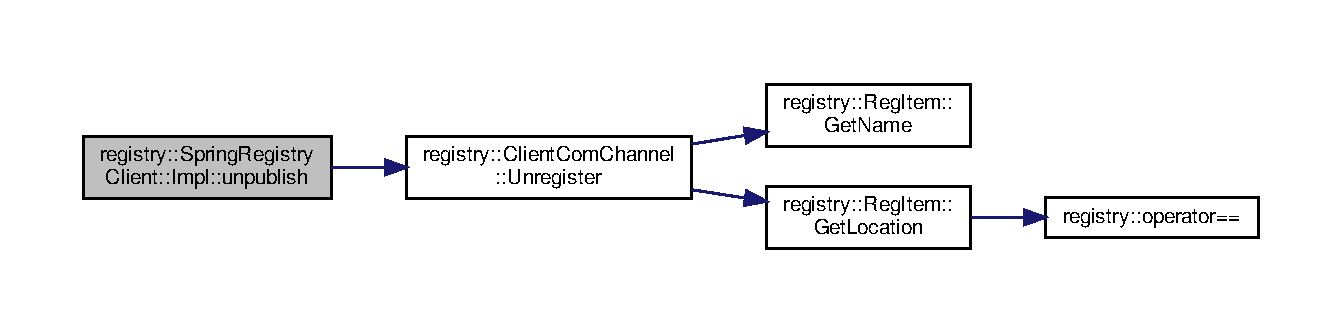
\includegraphics[width=350pt]{classregistry_1_1SpringRegistryClient_1_1Impl_ac3b721317dfb893e191d3d112575a627_cgraph}
\end{center}
\end{figure}


\subsection{Member Data Documentation}
\mbox{\Hypertarget{classregistry_1_1SpringRegistryClient_1_1Impl_ab0b715b0d49462786aa052d732f8207c}\label{classregistry_1_1SpringRegistryClient_1_1Impl_ab0b715b0d49462786aa052d732f8207c}} 
\index{registry\+::\+Spring\+Registry\+Client\+::\+Impl@{registry\+::\+Spring\+Registry\+Client\+::\+Impl}!clnt\+\_\+@{clnt\+\_\+}}
\index{clnt\+\_\+@{clnt\+\_\+}!registry\+::\+Spring\+Registry\+Client\+::\+Impl@{registry\+::\+Spring\+Registry\+Client\+::\+Impl}}
\subsubsection{\texorpdfstring{clnt\+\_\+}{clnt\_}}
{\footnotesize\ttfamily \hyperlink{classregistry_1_1ClientComChannel}{Client\+Com\+Channel} const registry\+::\+Spring\+Registry\+Client\+::\+Impl\+::clnt\+\_\+\hspace{0.3cm}{\ttfamily [private]}}

\mbox{\Hypertarget{classregistry_1_1SpringRegistryClient_1_1Impl_ad1c90e7182c68d7d48702d8b8329e805}\label{classregistry_1_1SpringRegistryClient_1_1Impl_ad1c90e7182c68d7d48702d8b8329e805}} 
\index{registry\+::\+Spring\+Registry\+Client\+::\+Impl@{registry\+::\+Spring\+Registry\+Client\+::\+Impl}!name\+\_\+@{name\+\_\+}}
\index{name\+\_\+@{name\+\_\+}!registry\+::\+Spring\+Registry\+Client\+::\+Impl@{registry\+::\+Spring\+Registry\+Client\+::\+Impl}}
\subsubsection{\texorpdfstring{name\+\_\+}{name\_}}
{\footnotesize\ttfamily std\+::string const registry\+::\+Spring\+Registry\+Client\+::\+Impl\+::name\+\_\+\hspace{0.3cm}{\ttfamily [private]}}



The documentation for this class was generated from the following file\+:\begin{DoxyCompactItemize}
\item 
registry/src/\hyperlink{registry__client__lib_8cpp}{registry\+\_\+client\+\_\+lib.\+cpp}\end{DoxyCompactItemize}

\hypertarget{classregistry_1_1ExtractorRegistryClient_1_1Impl}{}\section{registry\+:\+:Extractor\+Registry\+Client\+:\+:Impl Class Reference}
\label{classregistry_1_1ExtractorRegistryClient_1_1Impl}\index{registry\+::\+Extractor\+Registry\+Client\+::\+Impl@{registry\+::\+Extractor\+Registry\+Client\+::\+Impl}}


Collaboration diagram for registry\+:\+:Extractor\+Registry\+Client\+:\+:Impl\+:\nopagebreak
\begin{figure}[H]
\begin{center}
\leavevmode
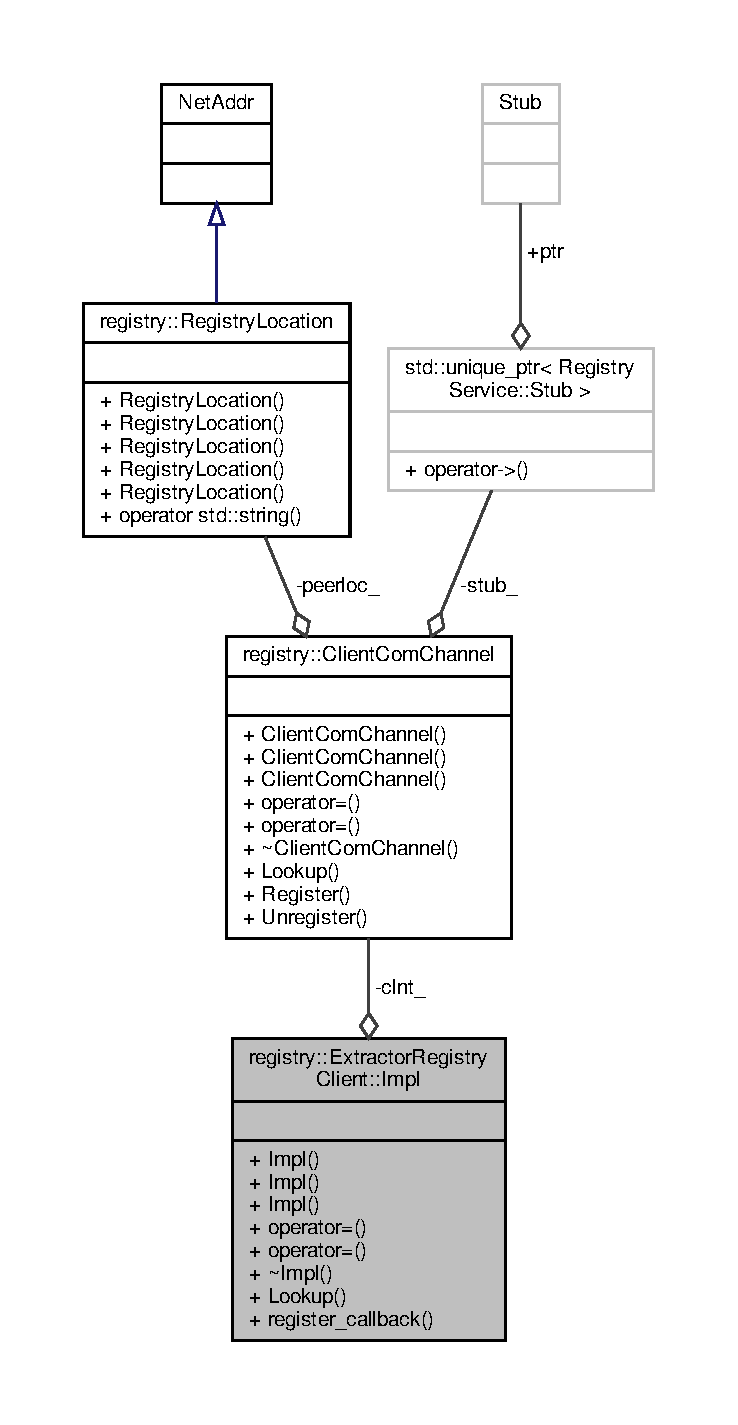
\includegraphics[height=550pt]{classregistry_1_1ExtractorRegistryClient_1_1Impl__coll__graph}
\end{center}
\end{figure}
\subsection*{Public Member Functions}
\begin{DoxyCompactItemize}
\item 
\hyperlink{classregistry_1_1ExtractorRegistryClient_1_1Impl_a17b812f50e898dafa7bd55ab32f682de}{Impl} (\hyperlink{structregistry_1_1RegistryLocation}{Registry\+Location} const \&l)
\item 
\hyperlink{classregistry_1_1ExtractorRegistryClient_1_1Impl_a40b247abc37f752c4692dc9ef01766d7}{Impl} (\hyperlink{classregistry_1_1ExtractorRegistryClient_1_1Impl}{Impl} const \&)=delete
\item 
\hyperlink{classregistry_1_1ExtractorRegistryClient_1_1Impl_ae20ac835c7ed8b4bf0551aa2966d9c72}{Impl} (\hyperlink{classregistry_1_1ExtractorRegistryClient_1_1Impl}{Impl} \&\&)=delete
\item 
\hyperlink{classregistry_1_1ExtractorRegistryClient_1_1Impl}{Impl} \& \hyperlink{classregistry_1_1ExtractorRegistryClient_1_1Impl_aa074380885dd859576d3dec0bb6428fd}{operator=} (\hyperlink{classregistry_1_1ExtractorRegistryClient_1_1Impl}{Impl} const \&)=delete
\item 
\hyperlink{classregistry_1_1ExtractorRegistryClient_1_1Impl}{Impl} \& \hyperlink{classregistry_1_1ExtractorRegistryClient_1_1Impl_aada6bfc4a190dc51f62f1ab00b9159af}{operator=} (\hyperlink{classregistry_1_1ExtractorRegistryClient_1_1Impl}{Impl} \&\&)=delete
\item 
\hyperlink{classregistry_1_1ExtractorRegistryClient_1_1Impl_af0aefd3ed554aa762e2458926a74602b}{$\sim$\+Impl} () noexcept=default
\item 
std\+::vector$<$ \hyperlink{classregistry_1_1RegItem}{Reg\+Item} $>$ \hyperlink{classregistry_1_1ExtractorRegistryClient_1_1Impl_aee705dc8ca2a3056bbb45ef25c57de16}{Lookup} (\hyperlink{classregistry_1_1Filter}{Filter} const \&) const
\item 
void \hyperlink{classregistry_1_1ExtractorRegistryClient_1_1Impl_aa85c7398b9da00a5eb35b9373b4a755d}{register\+\_\+callback} (\hyperlink{classregistry_1_1Filter}{Filter} const flt, std\+::function$<$ void()$>$ cb)
\end{DoxyCompactItemize}
\subsection*{Private Attributes}
\begin{DoxyCompactItemize}
\item 
\hyperlink{classregistry_1_1ClientComChannel}{Client\+Com\+Channel} const \hyperlink{classregistry_1_1ExtractorRegistryClient_1_1Impl_a702a01fb0fd983dbe146eb358736abd0}{clnt\+\_\+}
\end{DoxyCompactItemize}


\subsection{Constructor \& Destructor Documentation}
\mbox{\Hypertarget{classregistry_1_1ExtractorRegistryClient_1_1Impl_a17b812f50e898dafa7bd55ab32f682de}\label{classregistry_1_1ExtractorRegistryClient_1_1Impl_a17b812f50e898dafa7bd55ab32f682de}} 
\index{registry\+::\+Extractor\+Registry\+Client\+::\+Impl@{registry\+::\+Extractor\+Registry\+Client\+::\+Impl}!Impl@{Impl}}
\index{Impl@{Impl}!registry\+::\+Extractor\+Registry\+Client\+::\+Impl@{registry\+::\+Extractor\+Registry\+Client\+::\+Impl}}
\subsubsection{\texorpdfstring{Impl()}{Impl()}\hspace{0.1cm}{\footnotesize\ttfamily [1/3]}}
{\footnotesize\ttfamily registry\+::\+Extractor\+Registry\+Client\+::\+Impl\+::\+Impl (\begin{DoxyParamCaption}\item[{\hyperlink{structregistry_1_1RegistryLocation}{Registry\+Location} const \&}]{l }\end{DoxyParamCaption})}

\mbox{\Hypertarget{classregistry_1_1ExtractorRegistryClient_1_1Impl_a40b247abc37f752c4692dc9ef01766d7}\label{classregistry_1_1ExtractorRegistryClient_1_1Impl_a40b247abc37f752c4692dc9ef01766d7}} 
\index{registry\+::\+Extractor\+Registry\+Client\+::\+Impl@{registry\+::\+Extractor\+Registry\+Client\+::\+Impl}!Impl@{Impl}}
\index{Impl@{Impl}!registry\+::\+Extractor\+Registry\+Client\+::\+Impl@{registry\+::\+Extractor\+Registry\+Client\+::\+Impl}}
\subsubsection{\texorpdfstring{Impl()}{Impl()}\hspace{0.1cm}{\footnotesize\ttfamily [2/3]}}
{\footnotesize\ttfamily registry\+::\+Extractor\+Registry\+Client\+::\+Impl\+::\+Impl (\begin{DoxyParamCaption}\item[{\hyperlink{classregistry_1_1ExtractorRegistryClient_1_1Impl}{Impl} const \&}]{ }\end{DoxyParamCaption})\hspace{0.3cm}{\ttfamily [delete]}}

\mbox{\Hypertarget{classregistry_1_1ExtractorRegistryClient_1_1Impl_ae20ac835c7ed8b4bf0551aa2966d9c72}\label{classregistry_1_1ExtractorRegistryClient_1_1Impl_ae20ac835c7ed8b4bf0551aa2966d9c72}} 
\index{registry\+::\+Extractor\+Registry\+Client\+::\+Impl@{registry\+::\+Extractor\+Registry\+Client\+::\+Impl}!Impl@{Impl}}
\index{Impl@{Impl}!registry\+::\+Extractor\+Registry\+Client\+::\+Impl@{registry\+::\+Extractor\+Registry\+Client\+::\+Impl}}
\subsubsection{\texorpdfstring{Impl()}{Impl()}\hspace{0.1cm}{\footnotesize\ttfamily [3/3]}}
{\footnotesize\ttfamily registry\+::\+Extractor\+Registry\+Client\+::\+Impl\+::\+Impl (\begin{DoxyParamCaption}\item[{\hyperlink{classregistry_1_1ExtractorRegistryClient_1_1Impl}{Impl} \&\&}]{ }\end{DoxyParamCaption})\hspace{0.3cm}{\ttfamily [delete]}}

\mbox{\Hypertarget{classregistry_1_1ExtractorRegistryClient_1_1Impl_af0aefd3ed554aa762e2458926a74602b}\label{classregistry_1_1ExtractorRegistryClient_1_1Impl_af0aefd3ed554aa762e2458926a74602b}} 
\index{registry\+::\+Extractor\+Registry\+Client\+::\+Impl@{registry\+::\+Extractor\+Registry\+Client\+::\+Impl}!````~Impl@{$\sim$\+Impl}}
\index{````~Impl@{$\sim$\+Impl}!registry\+::\+Extractor\+Registry\+Client\+::\+Impl@{registry\+::\+Extractor\+Registry\+Client\+::\+Impl}}
\subsubsection{\texorpdfstring{$\sim$\+Impl()}{~Impl()}}
{\footnotesize\ttfamily registry\+::\+Extractor\+Registry\+Client\+::\+Impl\+::$\sim$\+Impl (\begin{DoxyParamCaption}{ }\end{DoxyParamCaption})\hspace{0.3cm}{\ttfamily [default]}, {\ttfamily [noexcept]}}



\subsection{Member Function Documentation}
\mbox{\Hypertarget{classregistry_1_1ExtractorRegistryClient_1_1Impl_aee705dc8ca2a3056bbb45ef25c57de16}\label{classregistry_1_1ExtractorRegistryClient_1_1Impl_aee705dc8ca2a3056bbb45ef25c57de16}} 
\index{registry\+::\+Extractor\+Registry\+Client\+::\+Impl@{registry\+::\+Extractor\+Registry\+Client\+::\+Impl}!Lookup@{Lookup}}
\index{Lookup@{Lookup}!registry\+::\+Extractor\+Registry\+Client\+::\+Impl@{registry\+::\+Extractor\+Registry\+Client\+::\+Impl}}
\subsubsection{\texorpdfstring{Lookup()}{Lookup()}}
{\footnotesize\ttfamily std\+::vector$<$ \hyperlink{classregistry_1_1RegItem}{Reg\+Item} $>$ registry\+::\+Extractor\+Registry\+Client\+::\+Impl\+::\+Lookup (\begin{DoxyParamCaption}\item[{\hyperlink{classregistry_1_1Filter}{Filter} const \&}]{fltr }\end{DoxyParamCaption}) const}

Here is the call graph for this function\+:
\nopagebreak
\begin{figure}[H]
\begin{center}
\leavevmode
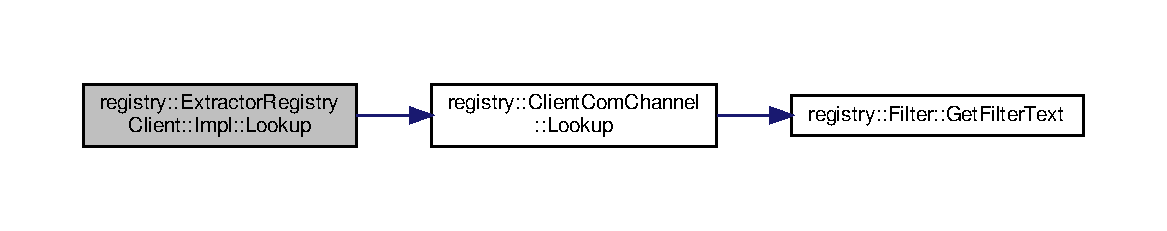
\includegraphics[width=350pt]{classregistry_1_1ExtractorRegistryClient_1_1Impl_aee705dc8ca2a3056bbb45ef25c57de16_cgraph}
\end{center}
\end{figure}
\mbox{\Hypertarget{classregistry_1_1ExtractorRegistryClient_1_1Impl_aa074380885dd859576d3dec0bb6428fd}\label{classregistry_1_1ExtractorRegistryClient_1_1Impl_aa074380885dd859576d3dec0bb6428fd}} 
\index{registry\+::\+Extractor\+Registry\+Client\+::\+Impl@{registry\+::\+Extractor\+Registry\+Client\+::\+Impl}!operator=@{operator=}}
\index{operator=@{operator=}!registry\+::\+Extractor\+Registry\+Client\+::\+Impl@{registry\+::\+Extractor\+Registry\+Client\+::\+Impl}}
\subsubsection{\texorpdfstring{operator=()}{operator=()}\hspace{0.1cm}{\footnotesize\ttfamily [1/2]}}
{\footnotesize\ttfamily \hyperlink{classregistry_1_1ExtractorRegistryClient_1_1Impl}{Impl}\& registry\+::\+Extractor\+Registry\+Client\+::\+Impl\+::operator= (\begin{DoxyParamCaption}\item[{\hyperlink{classregistry_1_1ExtractorRegistryClient_1_1Impl}{Impl} const \&}]{ }\end{DoxyParamCaption})\hspace{0.3cm}{\ttfamily [delete]}}

\mbox{\Hypertarget{classregistry_1_1ExtractorRegistryClient_1_1Impl_aada6bfc4a190dc51f62f1ab00b9159af}\label{classregistry_1_1ExtractorRegistryClient_1_1Impl_aada6bfc4a190dc51f62f1ab00b9159af}} 
\index{registry\+::\+Extractor\+Registry\+Client\+::\+Impl@{registry\+::\+Extractor\+Registry\+Client\+::\+Impl}!operator=@{operator=}}
\index{operator=@{operator=}!registry\+::\+Extractor\+Registry\+Client\+::\+Impl@{registry\+::\+Extractor\+Registry\+Client\+::\+Impl}}
\subsubsection{\texorpdfstring{operator=()}{operator=()}\hspace{0.1cm}{\footnotesize\ttfamily [2/2]}}
{\footnotesize\ttfamily \hyperlink{classregistry_1_1ExtractorRegistryClient_1_1Impl}{Impl}\& registry\+::\+Extractor\+Registry\+Client\+::\+Impl\+::operator= (\begin{DoxyParamCaption}\item[{\hyperlink{classregistry_1_1ExtractorRegistryClient_1_1Impl}{Impl} \&\&}]{ }\end{DoxyParamCaption})\hspace{0.3cm}{\ttfamily [delete]}}

\mbox{\Hypertarget{classregistry_1_1ExtractorRegistryClient_1_1Impl_aa85c7398b9da00a5eb35b9373b4a755d}\label{classregistry_1_1ExtractorRegistryClient_1_1Impl_aa85c7398b9da00a5eb35b9373b4a755d}} 
\index{registry\+::\+Extractor\+Registry\+Client\+::\+Impl@{registry\+::\+Extractor\+Registry\+Client\+::\+Impl}!register\+\_\+callback@{register\+\_\+callback}}
\index{register\+\_\+callback@{register\+\_\+callback}!registry\+::\+Extractor\+Registry\+Client\+::\+Impl@{registry\+::\+Extractor\+Registry\+Client\+::\+Impl}}
\subsubsection{\texorpdfstring{register\+\_\+callback()}{register\_callback()}}
{\footnotesize\ttfamily void registry\+::\+Extractor\+Registry\+Client\+::\+Impl\+::register\+\_\+callback (\begin{DoxyParamCaption}\item[{\hyperlink{classregistry_1_1Filter}{Filter} const}]{flt,  }\item[{std\+::function$<$ void()$>$}]{cb }\end{DoxyParamCaption})}



\subsection{Member Data Documentation}
\mbox{\Hypertarget{classregistry_1_1ExtractorRegistryClient_1_1Impl_a702a01fb0fd983dbe146eb358736abd0}\label{classregistry_1_1ExtractorRegistryClient_1_1Impl_a702a01fb0fd983dbe146eb358736abd0}} 
\index{registry\+::\+Extractor\+Registry\+Client\+::\+Impl@{registry\+::\+Extractor\+Registry\+Client\+::\+Impl}!clnt\+\_\+@{clnt\+\_\+}}
\index{clnt\+\_\+@{clnt\+\_\+}!registry\+::\+Extractor\+Registry\+Client\+::\+Impl@{registry\+::\+Extractor\+Registry\+Client\+::\+Impl}}
\subsubsection{\texorpdfstring{clnt\+\_\+}{clnt\_}}
{\footnotesize\ttfamily \hyperlink{classregistry_1_1ClientComChannel}{Client\+Com\+Channel} const registry\+::\+Extractor\+Registry\+Client\+::\+Impl\+::clnt\+\_\+\hspace{0.3cm}{\ttfamily [private]}}



The documentation for this class was generated from the following file\+:\begin{DoxyCompactItemize}
\item 
registry/src/\hyperlink{registry__client__lib_8cpp}{registry\+\_\+client\+\_\+lib.\+cpp}\end{DoxyCompactItemize}

\hypertarget{classregistry_1_1LookupFailed}{}\section{registry\+:\+:Lookup\+Failed Class Reference}
\label{classregistry_1_1LookupFailed}\index{registry\+::\+Lookup\+Failed@{registry\+::\+Lookup\+Failed}}


Thrown when the g\+R\+PC stub returns any error status in responce to a Lookup request.  




{\ttfamily \#include $<$registry\+\_\+common.\+hpp$>$}



Inheritance diagram for registry\+:\+:Lookup\+Failed\+:
\nopagebreak
\begin{figure}[H]
\begin{center}
\leavevmode
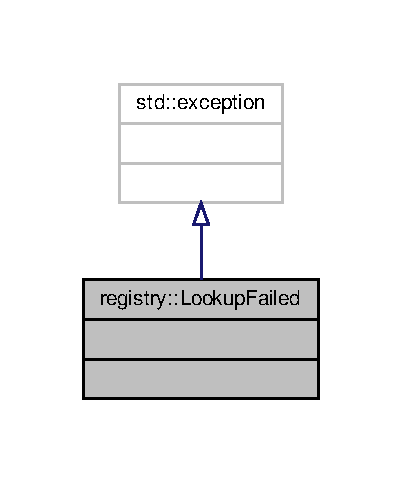
\includegraphics[width=193pt]{classregistry_1_1LookupFailed__inherit__graph}
\end{center}
\end{figure}


Collaboration diagram for registry\+:\+:Lookup\+Failed\+:
\nopagebreak
\begin{figure}[H]
\begin{center}
\leavevmode
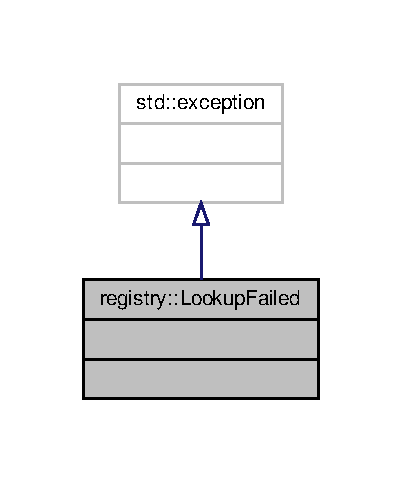
\includegraphics[width=193pt]{classregistry_1_1LookupFailed__coll__graph}
\end{center}
\end{figure}


\subsection{Detailed Description}
Thrown when the g\+R\+PC stub returns any error status in responce to a Lookup request. 

The documentation for this class was generated from the following file\+:\begin{DoxyCompactItemize}
\item 
registry/include/\hyperlink{registry__common_8hpp}{registry\+\_\+common.\+hpp}\end{DoxyCompactItemize}

\hypertarget{classNetAddr}{}\section{Net\+Addr Class Reference}
\label{classNetAddr}\index{Net\+Addr@{Net\+Addr}}


Inheritance diagram for Net\+Addr\+:\nopagebreak
\begin{figure}[H]
\begin{center}
\leavevmode
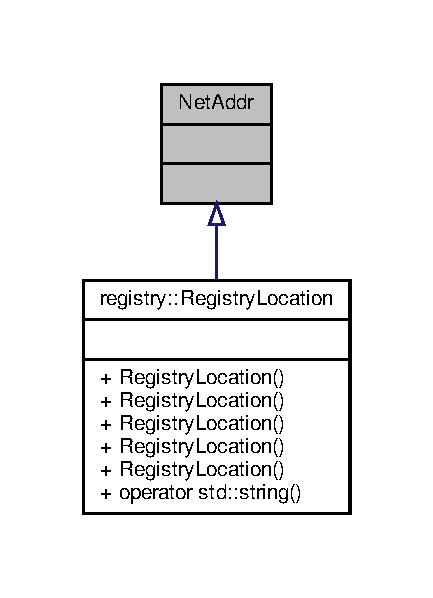
\includegraphics[width=208pt]{classNetAddr__inherit__graph}
\end{center}
\end{figure}


Collaboration diagram for Net\+Addr\+:\nopagebreak
\begin{figure}[H]
\begin{center}
\leavevmode
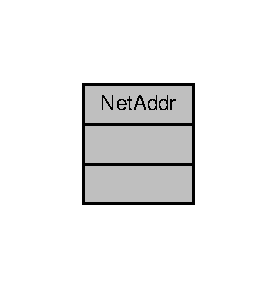
\includegraphics[width=133pt]{classNetAddr__coll__graph}
\end{center}
\end{figure}


The documentation for this class was generated from the following file\+:\begin{DoxyCompactItemize}
\item 
registry/include/\hyperlink{registry__common_8hpp}{registry\+\_\+common.\+hpp}\end{DoxyCompactItemize}

\hypertarget{structregistry_1_1RegistrationException}{}\section{registry\+:\+:Registration\+Exception Struct Reference}
\label{structregistry_1_1RegistrationException}\index{registry\+::\+Registration\+Exception@{registry\+::\+Registration\+Exception}}


{\ttfamily \#include $<$registry\+\_\+client.\+hpp$>$}



Inheritance diagram for registry\+:\+:Registration\+Exception\+:\nopagebreak
\begin{figure}[H]
\begin{center}
\leavevmode
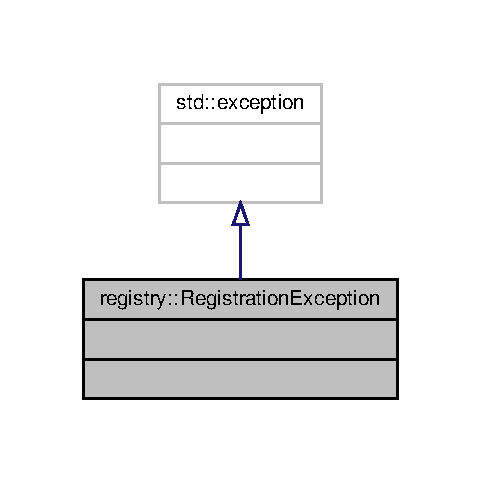
\includegraphics[width=231pt]{structregistry_1_1RegistrationException__inherit__graph}
\end{center}
\end{figure}


Collaboration diagram for registry\+:\+:Registration\+Exception\+:\nopagebreak
\begin{figure}[H]
\begin{center}
\leavevmode
\includegraphics[width=231pt]{structregistry_1_1RegistrationException__coll__graph}
\end{center}
\end{figure}


\subsection{Detailed Description}
This exception is throw to indicate that the g\+R\+PC stub has returned an error status in response to a Registration request. 

The documentation for this struct was generated from the following file\+:\begin{DoxyCompactItemize}
\item 
registry/include/\hyperlink{registry__client_8hpp}{registry\+\_\+client.\+hpp}\end{DoxyCompactItemize}

\hypertarget{classregistry_1_1RegistrationFailed}{}\section{registry\+:\+:Registration\+Failed Class Reference}
\label{classregistry_1_1RegistrationFailed}\index{registry\+::\+Registration\+Failed@{registry\+::\+Registration\+Failed}}


{\ttfamily \#include $<$registry\+\_\+core.\+hpp$>$}



Inheritance diagram for registry\+:\+:Registration\+Failed\+:\nopagebreak
\begin{figure}[H]
\begin{center}
\leavevmode
\includegraphics[width=214pt]{classregistry_1_1RegistrationFailed__inherit__graph}
\end{center}
\end{figure}


Collaboration diagram for registry\+:\+:Registration\+Failed\+:\nopagebreak
\begin{figure}[H]
\begin{center}
\leavevmode
\includegraphics[width=214pt]{classregistry_1_1RegistrationFailed__coll__graph}
\end{center}
\end{figure}


The documentation for this class was generated from the following file\+:\begin{DoxyCompactItemize}
\item 
registry/src/\hyperlink{registry__core_8hpp}{registry\+\_\+core.\+hpp}\end{DoxyCompactItemize}

\hypertarget{classregistry_1_1RegistryImplSQLite}{}\section{registry\+:\+:Registry\+Impl\+S\+Q\+Lite Class Reference}
\label{classregistry_1_1RegistryImplSQLite}\index{registry\+::\+Registry\+Impl\+S\+Q\+Lite@{registry\+::\+Registry\+Impl\+S\+Q\+Lite}}


{\ttfamily \#include $<$registry\+\_\+core.\+hpp$>$}



Collaboration diagram for registry\+:\+:Registry\+Impl\+S\+Q\+Lite\+:
\nopagebreak
\begin{figure}[H]
\begin{center}
\leavevmode
\includegraphics[width=350pt]{classregistry_1_1RegistryImplSQLite__coll__graph}
\end{center}
\end{figure}
\subsection*{Public Member Functions}
\begin{DoxyCompactItemize}
\item 
\hyperlink{classregistry_1_1RegistryImplSQLite_ad211242bf6438adad6ad01c3d5863f6f}{Registry\+Impl\+S\+Q\+Lite} (std\+::string db\+\_\+path)
\item 
\hyperlink{classregistry_1_1RegistryImplSQLite_a5d57b3f718213a7b8fbdc46e09b213af}{$\sim$\+Registry\+Impl\+S\+Q\+Lite} ()
\item 
void \hyperlink{classregistry_1_1RegistryImplSQLite_ac7781e882e1e072fde41ced3842eec6c}{Register} (\hyperlink{classregistry_1_1RegItem}{Reg\+Item} ri)
\item 
void \hyperlink{classregistry_1_1RegistryImplSQLite_aed678237358b3024a2afe2d4585e0c54}{Unregister} (\hyperlink{classregistry_1_1RegItem}{Reg\+Item} ri)
\item 
void \hyperlink{classregistry_1_1RegistryImplSQLite_ad9579736bcded70177bf9d8862cb79a0}{Add\+Callback} (\hyperlink{classregistry_1_1Filter}{Filter} flt, \hyperlink{classregistry_1_1AbstractRegistry_a08a798ca9ca1c4c983ebd2386ca3c315}{Abstract\+Registry\+::\+Callback} cb)
\item 
void \hyperlink{classregistry_1_1RegistryImplSQLite_a45b864d4111f994db1febfc622a83334}{Remove\+Callback} (\hyperlink{classregistry_1_1Filter}{Filter} flt, \hyperlink{classregistry_1_1AbstractRegistry_a08a798ca9ca1c4c983ebd2386ca3c315}{Abstract\+Registry\+::\+Callback} cb)
\item 
std\+::vector$<$ \hyperlink{classregistry_1_1RegItem}{Reg\+Item} $>$ \hyperlink{classregistry_1_1RegistryImplSQLite_ac2c846357de9bc83654193057a7edca1}{Lookup} (\hyperlink{classregistry_1_1Filter}{Filter} flt)
\end{DoxyCompactItemize}
\subsection*{Private Member Functions}
\begin{DoxyCompactItemize}
\item 
std\+::vector$<$ \hyperlink{classregistry_1_1RegItem}{Reg\+Item} $>$ \hyperlink{classregistry_1_1RegistryImplSQLite_a567444904255035f5b13feb8fd4c3ddd}{Check\+Filters} (void)
\item 
std\+::vector$<$ \hyperlink{classregistry_1_1RegItem}{Reg\+Item} $>$ \hyperlink{classregistry_1_1RegistryImplSQLite_a75eb46a6b3fb0f1abd01e409d989462d}{Check\+Filters} (\hyperlink{classregistry_1_1Filter}{Filter} const flt)
\item 
int \hyperlink{classregistry_1_1RegistryImplSQLite_a09fbc2f21027ef2d129350173fc81c61}{Check\+Callbacks} (void)
\item 
int \hyperlink{classregistry_1_1RegistryImplSQLite_af65ab0ea80408ceb2f18705ca8f3a463}{Check\+Callbacks} (\hyperlink{classregistry_1_1AbstractRegistry_a31f6bef634dcd324efebaf55f99b950f}{Abstract\+Registry\+::\+Filter\+Callback} const \&fcb)
\item 
int \hyperlink{classregistry_1_1RegistryImplSQLite_abca7604f13519e5a93632550e7b309dd}{Check\+Callbacks} (\hyperlink{classregistry_1_1RegItem}{Reg\+Item} const \&ri)
\item 
void \hyperlink{classregistry_1_1RegistryImplSQLite_a4a9f3255a1af40969b914e3bc5707874}{Init\+Db} ()
\item 
bool \hyperlink{classregistry_1_1RegistryImplSQLite_afa1e3fb05442de7d3d13887e33b972c0}{Check\+Db} ()
\item 
bool \hyperlink{classregistry_1_1RegistryImplSQLite_ab3bfdd5ea39fb7b0a4e621a082ddece1}{Sql\+Select\+In\+Db} (std\+::string criteria, std\+::vector$<$ \hyperlink{classregistry_1_1RegItem}{Reg\+Item} $>$ \&matches)
\end{DoxyCompactItemize}
\subsection*{Private Attributes}
\begin{DoxyCompactItemize}
\item 
sqlite3 $\ast$ \hyperlink{classregistry_1_1RegistryImplSQLite_af79b30f624a35f84e585a72b2212d5fc}{db\+\_\+}
\item 
std\+::string const \hyperlink{classregistry_1_1RegistryImplSQLite_abe58267856da3b53b03834a2b177007d}{k\+Items\+Table\+Name} = \char`\"{}I\+T\+E\+MS\char`\"{}
\item 
std\+::vector$<$ \hyperlink{classregistry_1_1AbstractRegistry_a31f6bef634dcd324efebaf55f99b950f}{Abstract\+Registry\+::\+Filter\+Callback} $>$ \hyperlink{classregistry_1_1RegistryImplSQLite_a39709978c5bc5828fee650690aa9d8ad}{callbacks\+\_\+}
\item 
std\+::shared\+\_\+mutex \hyperlink{classregistry_1_1RegistryImplSQLite_a7c0db71680eb0ccd8b24d315e5b6b053}{items\+\_\+lock\+\_\+}
\item 
std\+::shared\+\_\+mutex \hyperlink{classregistry_1_1RegistryImplSQLite_ac6bcca9380e8c6ba7cef152392043ebd}{callbacks\+\_\+lock\+\_\+}
\end{DoxyCompactItemize}


\subsection{Constructor \& Destructor Documentation}
\mbox{\Hypertarget{classregistry_1_1RegistryImplSQLite_ad211242bf6438adad6ad01c3d5863f6f}\label{classregistry_1_1RegistryImplSQLite_ad211242bf6438adad6ad01c3d5863f6f}} 
\index{registry\+::\+Registry\+Impl\+S\+Q\+Lite@{registry\+::\+Registry\+Impl\+S\+Q\+Lite}!Registry\+Impl\+S\+Q\+Lite@{Registry\+Impl\+S\+Q\+Lite}}
\index{Registry\+Impl\+S\+Q\+Lite@{Registry\+Impl\+S\+Q\+Lite}!registry\+::\+Registry\+Impl\+S\+Q\+Lite@{registry\+::\+Registry\+Impl\+S\+Q\+Lite}}
\subsubsection{\texorpdfstring{Registry\+Impl\+S\+Q\+Lite()}{RegistryImplSQLite()}}
{\footnotesize\ttfamily registry\+::\+Registry\+Impl\+S\+Q\+Lite\+::\+Registry\+Impl\+S\+Q\+Lite (\begin{DoxyParamCaption}\item[{std\+::string}]{db\+\_\+path = {\ttfamily \char`\"{}registry.sqlite\char`\"{}} }\end{DoxyParamCaption})\hspace{0.3cm}{\ttfamily [inline]}}

\mbox{\Hypertarget{classregistry_1_1RegistryImplSQLite_a5d57b3f718213a7b8fbdc46e09b213af}\label{classregistry_1_1RegistryImplSQLite_a5d57b3f718213a7b8fbdc46e09b213af}} 
\index{registry\+::\+Registry\+Impl\+S\+Q\+Lite@{registry\+::\+Registry\+Impl\+S\+Q\+Lite}!````~Registry\+Impl\+S\+Q\+Lite@{$\sim$\+Registry\+Impl\+S\+Q\+Lite}}
\index{````~Registry\+Impl\+S\+Q\+Lite@{$\sim$\+Registry\+Impl\+S\+Q\+Lite}!registry\+::\+Registry\+Impl\+S\+Q\+Lite@{registry\+::\+Registry\+Impl\+S\+Q\+Lite}}
\subsubsection{\texorpdfstring{$\sim$\+Registry\+Impl\+S\+Q\+Lite()}{~RegistryImplSQLite()}}
{\footnotesize\ttfamily registry\+::\+Registry\+Impl\+S\+Q\+Lite\+::$\sim$\+Registry\+Impl\+S\+Q\+Lite (\begin{DoxyParamCaption}{ }\end{DoxyParamCaption})}



\subsection{Member Function Documentation}
\mbox{\Hypertarget{classregistry_1_1RegistryImplSQLite_ad9579736bcded70177bf9d8862cb79a0}\label{classregistry_1_1RegistryImplSQLite_ad9579736bcded70177bf9d8862cb79a0}} 
\index{registry\+::\+Registry\+Impl\+S\+Q\+Lite@{registry\+::\+Registry\+Impl\+S\+Q\+Lite}!Add\+Callback@{Add\+Callback}}
\index{Add\+Callback@{Add\+Callback}!registry\+::\+Registry\+Impl\+S\+Q\+Lite@{registry\+::\+Registry\+Impl\+S\+Q\+Lite}}
\subsubsection{\texorpdfstring{Add\+Callback()}{AddCallback()}}
{\footnotesize\ttfamily void registry\+::\+Registry\+Impl\+S\+Q\+Lite\+::\+Add\+Callback (\begin{DoxyParamCaption}\item[{\hyperlink{classregistry_1_1Filter}{Filter}}]{flt,  }\item[{\hyperlink{classregistry_1_1AbstractRegistry_a08a798ca9ca1c4c983ebd2386ca3c315}{Abstract\+Registry\+::\+Callback}}]{cb }\end{DoxyParamCaption})\hspace{0.3cm}{\ttfamily [inline]}}

\mbox{\Hypertarget{classregistry_1_1RegistryImplSQLite_a09fbc2f21027ef2d129350173fc81c61}\label{classregistry_1_1RegistryImplSQLite_a09fbc2f21027ef2d129350173fc81c61}} 
\index{registry\+::\+Registry\+Impl\+S\+Q\+Lite@{registry\+::\+Registry\+Impl\+S\+Q\+Lite}!Check\+Callbacks@{Check\+Callbacks}}
\index{Check\+Callbacks@{Check\+Callbacks}!registry\+::\+Registry\+Impl\+S\+Q\+Lite@{registry\+::\+Registry\+Impl\+S\+Q\+Lite}}
\subsubsection{\texorpdfstring{Check\+Callbacks()}{CheckCallbacks()}\hspace{0.1cm}{\footnotesize\ttfamily [1/3]}}
{\footnotesize\ttfamily int registry\+::\+Registry\+Impl\+S\+Q\+Lite\+::\+Check\+Callbacks (\begin{DoxyParamCaption}\item[{void}]{ }\end{DoxyParamCaption})\hspace{0.3cm}{\ttfamily [private]}}

\mbox{\Hypertarget{classregistry_1_1RegistryImplSQLite_af65ab0ea80408ceb2f18705ca8f3a463}\label{classregistry_1_1RegistryImplSQLite_af65ab0ea80408ceb2f18705ca8f3a463}} 
\index{registry\+::\+Registry\+Impl\+S\+Q\+Lite@{registry\+::\+Registry\+Impl\+S\+Q\+Lite}!Check\+Callbacks@{Check\+Callbacks}}
\index{Check\+Callbacks@{Check\+Callbacks}!registry\+::\+Registry\+Impl\+S\+Q\+Lite@{registry\+::\+Registry\+Impl\+S\+Q\+Lite}}
\subsubsection{\texorpdfstring{Check\+Callbacks()}{CheckCallbacks()}\hspace{0.1cm}{\footnotesize\ttfamily [2/3]}}
{\footnotesize\ttfamily int registry\+::\+Registry\+Impl\+S\+Q\+Lite\+::\+Check\+Callbacks (\begin{DoxyParamCaption}\item[{\hyperlink{classregistry_1_1AbstractRegistry_a31f6bef634dcd324efebaf55f99b950f}{Abstract\+Registry\+::\+Filter\+Callback} const \&}]{fcb }\end{DoxyParamCaption})\hspace{0.3cm}{\ttfamily [private]}}

\mbox{\Hypertarget{classregistry_1_1RegistryImplSQLite_abca7604f13519e5a93632550e7b309dd}\label{classregistry_1_1RegistryImplSQLite_abca7604f13519e5a93632550e7b309dd}} 
\index{registry\+::\+Registry\+Impl\+S\+Q\+Lite@{registry\+::\+Registry\+Impl\+S\+Q\+Lite}!Check\+Callbacks@{Check\+Callbacks}}
\index{Check\+Callbacks@{Check\+Callbacks}!registry\+::\+Registry\+Impl\+S\+Q\+Lite@{registry\+::\+Registry\+Impl\+S\+Q\+Lite}}
\subsubsection{\texorpdfstring{Check\+Callbacks()}{CheckCallbacks()}\hspace{0.1cm}{\footnotesize\ttfamily [3/3]}}
{\footnotesize\ttfamily int registry\+::\+Registry\+Impl\+S\+Q\+Lite\+::\+Check\+Callbacks (\begin{DoxyParamCaption}\item[{\hyperlink{classregistry_1_1RegItem}{Reg\+Item} const \&}]{ri }\end{DoxyParamCaption})\hspace{0.3cm}{\ttfamily [private]}}

Here is the call graph for this function\+:
\nopagebreak
\begin{figure}[H]
\begin{center}
\leavevmode
\includegraphics[width=350pt]{classregistry_1_1RegistryImplSQLite_abca7604f13519e5a93632550e7b309dd_cgraph}
\end{center}
\end{figure}
\mbox{\Hypertarget{classregistry_1_1RegistryImplSQLite_afa1e3fb05442de7d3d13887e33b972c0}\label{classregistry_1_1RegistryImplSQLite_afa1e3fb05442de7d3d13887e33b972c0}} 
\index{registry\+::\+Registry\+Impl\+S\+Q\+Lite@{registry\+::\+Registry\+Impl\+S\+Q\+Lite}!Check\+Db@{Check\+Db}}
\index{Check\+Db@{Check\+Db}!registry\+::\+Registry\+Impl\+S\+Q\+Lite@{registry\+::\+Registry\+Impl\+S\+Q\+Lite}}
\subsubsection{\texorpdfstring{Check\+Db()}{CheckDb()}}
{\footnotesize\ttfamily bool registry\+::\+Registry\+Impl\+S\+Q\+Lite\+::\+Check\+Db (\begin{DoxyParamCaption}{ }\end{DoxyParamCaption})\hspace{0.3cm}{\ttfamily [private]}}

\mbox{\Hypertarget{classregistry_1_1RegistryImplSQLite_a567444904255035f5b13feb8fd4c3ddd}\label{classregistry_1_1RegistryImplSQLite_a567444904255035f5b13feb8fd4c3ddd}} 
\index{registry\+::\+Registry\+Impl\+S\+Q\+Lite@{registry\+::\+Registry\+Impl\+S\+Q\+Lite}!Check\+Filters@{Check\+Filters}}
\index{Check\+Filters@{Check\+Filters}!registry\+::\+Registry\+Impl\+S\+Q\+Lite@{registry\+::\+Registry\+Impl\+S\+Q\+Lite}}
\subsubsection{\texorpdfstring{Check\+Filters()}{CheckFilters()}\hspace{0.1cm}{\footnotesize\ttfamily [1/2]}}
{\footnotesize\ttfamily std\+::vector$<$ \hyperlink{classregistry_1_1RegItem}{Reg\+Item} $>$ registry\+::\+Registry\+Impl\+S\+Q\+Lite\+::\+Check\+Filters (\begin{DoxyParamCaption}\item[{void}]{ }\end{DoxyParamCaption})\hspace{0.3cm}{\ttfamily [private]}}

\mbox{\Hypertarget{classregistry_1_1RegistryImplSQLite_a75eb46a6b3fb0f1abd01e409d989462d}\label{classregistry_1_1RegistryImplSQLite_a75eb46a6b3fb0f1abd01e409d989462d}} 
\index{registry\+::\+Registry\+Impl\+S\+Q\+Lite@{registry\+::\+Registry\+Impl\+S\+Q\+Lite}!Check\+Filters@{Check\+Filters}}
\index{Check\+Filters@{Check\+Filters}!registry\+::\+Registry\+Impl\+S\+Q\+Lite@{registry\+::\+Registry\+Impl\+S\+Q\+Lite}}
\subsubsection{\texorpdfstring{Check\+Filters()}{CheckFilters()}\hspace{0.1cm}{\footnotesize\ttfamily [2/2]}}
{\footnotesize\ttfamily std\+::vector$<$ \hyperlink{classregistry_1_1RegItem}{Reg\+Item} $>$ registry\+::\+Registry\+Impl\+S\+Q\+Lite\+::\+Check\+Filters (\begin{DoxyParamCaption}\item[{\hyperlink{classregistry_1_1Filter}{Filter} const}]{flt }\end{DoxyParamCaption})\hspace{0.3cm}{\ttfamily [private]}}

Here is the call graph for this function\+:
\nopagebreak
\begin{figure}[H]
\begin{center}
\leavevmode
\includegraphics[width=350pt]{classregistry_1_1RegistryImplSQLite_a75eb46a6b3fb0f1abd01e409d989462d_cgraph}
\end{center}
\end{figure}
\mbox{\Hypertarget{classregistry_1_1RegistryImplSQLite_a4a9f3255a1af40969b914e3bc5707874}\label{classregistry_1_1RegistryImplSQLite_a4a9f3255a1af40969b914e3bc5707874}} 
\index{registry\+::\+Registry\+Impl\+S\+Q\+Lite@{registry\+::\+Registry\+Impl\+S\+Q\+Lite}!Init\+Db@{Init\+Db}}
\index{Init\+Db@{Init\+Db}!registry\+::\+Registry\+Impl\+S\+Q\+Lite@{registry\+::\+Registry\+Impl\+S\+Q\+Lite}}
\subsubsection{\texorpdfstring{Init\+Db()}{InitDb()}}
{\footnotesize\ttfamily void registry\+::\+Registry\+Impl\+S\+Q\+Lite\+::\+Init\+Db (\begin{DoxyParamCaption}{ }\end{DoxyParamCaption})\hspace{0.3cm}{\ttfamily [private]}}

\mbox{\Hypertarget{classregistry_1_1RegistryImplSQLite_ac2c846357de9bc83654193057a7edca1}\label{classregistry_1_1RegistryImplSQLite_ac2c846357de9bc83654193057a7edca1}} 
\index{registry\+::\+Registry\+Impl\+S\+Q\+Lite@{registry\+::\+Registry\+Impl\+S\+Q\+Lite}!Lookup@{Lookup}}
\index{Lookup@{Lookup}!registry\+::\+Registry\+Impl\+S\+Q\+Lite@{registry\+::\+Registry\+Impl\+S\+Q\+Lite}}
\subsubsection{\texorpdfstring{Lookup()}{Lookup()}}
{\footnotesize\ttfamily std\+::vector$<$ \hyperlink{classregistry_1_1RegItem}{Reg\+Item} $>$ registry\+::\+Registry\+Impl\+S\+Q\+Lite\+::\+Lookup (\begin{DoxyParamCaption}\item[{\hyperlink{classregistry_1_1Filter}{Filter}}]{flt }\end{DoxyParamCaption})\hspace{0.3cm}{\ttfamily [inline]}}

\mbox{\Hypertarget{classregistry_1_1RegistryImplSQLite_ac7781e882e1e072fde41ced3842eec6c}\label{classregistry_1_1RegistryImplSQLite_ac7781e882e1e072fde41ced3842eec6c}} 
\index{registry\+::\+Registry\+Impl\+S\+Q\+Lite@{registry\+::\+Registry\+Impl\+S\+Q\+Lite}!Register@{Register}}
\index{Register@{Register}!registry\+::\+Registry\+Impl\+S\+Q\+Lite@{registry\+::\+Registry\+Impl\+S\+Q\+Lite}}
\subsubsection{\texorpdfstring{Register()}{Register()}}
{\footnotesize\ttfamily void registry\+::\+Registry\+Impl\+S\+Q\+Lite\+::\+Register (\begin{DoxyParamCaption}\item[{\hyperlink{classregistry_1_1RegItem}{Reg\+Item}}]{ri }\end{DoxyParamCaption})\hspace{0.3cm}{\ttfamily [inline]}}

Here is the call graph for this function\+:
\nopagebreak
\begin{figure}[H]
\begin{center}
\leavevmode
\includegraphics[width=350pt]{classregistry_1_1RegistryImplSQLite_ac7781e882e1e072fde41ced3842eec6c_cgraph}
\end{center}
\end{figure}
\mbox{\Hypertarget{classregistry_1_1RegistryImplSQLite_a45b864d4111f994db1febfc622a83334}\label{classregistry_1_1RegistryImplSQLite_a45b864d4111f994db1febfc622a83334}} 
\index{registry\+::\+Registry\+Impl\+S\+Q\+Lite@{registry\+::\+Registry\+Impl\+S\+Q\+Lite}!Remove\+Callback@{Remove\+Callback}}
\index{Remove\+Callback@{Remove\+Callback}!registry\+::\+Registry\+Impl\+S\+Q\+Lite@{registry\+::\+Registry\+Impl\+S\+Q\+Lite}}
\subsubsection{\texorpdfstring{Remove\+Callback()}{RemoveCallback()}}
{\footnotesize\ttfamily void registry\+::\+Registry\+Impl\+S\+Q\+Lite\+::\+Remove\+Callback (\begin{DoxyParamCaption}\item[{\hyperlink{classregistry_1_1Filter}{Filter}}]{flt,  }\item[{\hyperlink{classregistry_1_1AbstractRegistry_a08a798ca9ca1c4c983ebd2386ca3c315}{Abstract\+Registry\+::\+Callback}}]{cb }\end{DoxyParamCaption})\hspace{0.3cm}{\ttfamily [inline]}}

\mbox{\Hypertarget{classregistry_1_1RegistryImplSQLite_ab3bfdd5ea39fb7b0a4e621a082ddece1}\label{classregistry_1_1RegistryImplSQLite_ab3bfdd5ea39fb7b0a4e621a082ddece1}} 
\index{registry\+::\+Registry\+Impl\+S\+Q\+Lite@{registry\+::\+Registry\+Impl\+S\+Q\+Lite}!Sql\+Select\+In\+Db@{Sql\+Select\+In\+Db}}
\index{Sql\+Select\+In\+Db@{Sql\+Select\+In\+Db}!registry\+::\+Registry\+Impl\+S\+Q\+Lite@{registry\+::\+Registry\+Impl\+S\+Q\+Lite}}
\subsubsection{\texorpdfstring{Sql\+Select\+In\+Db()}{SqlSelectInDb()}}
{\footnotesize\ttfamily bool registry\+::\+Registry\+Impl\+S\+Q\+Lite\+::\+Sql\+Select\+In\+Db (\begin{DoxyParamCaption}\item[{std\+::string}]{criteria,  }\item[{std\+::vector$<$ \hyperlink{classregistry_1_1RegItem}{Reg\+Item} $>$ \&}]{matches }\end{DoxyParamCaption})\hspace{0.3cm}{\ttfamily [private]}}

\mbox{\Hypertarget{classregistry_1_1RegistryImplSQLite_aed678237358b3024a2afe2d4585e0c54}\label{classregistry_1_1RegistryImplSQLite_aed678237358b3024a2afe2d4585e0c54}} 
\index{registry\+::\+Registry\+Impl\+S\+Q\+Lite@{registry\+::\+Registry\+Impl\+S\+Q\+Lite}!Unregister@{Unregister}}
\index{Unregister@{Unregister}!registry\+::\+Registry\+Impl\+S\+Q\+Lite@{registry\+::\+Registry\+Impl\+S\+Q\+Lite}}
\subsubsection{\texorpdfstring{Unregister()}{Unregister()}}
{\footnotesize\ttfamily void registry\+::\+Registry\+Impl\+S\+Q\+Lite\+::\+Unregister (\begin{DoxyParamCaption}\item[{\hyperlink{classregistry_1_1RegItem}{Reg\+Item}}]{ri }\end{DoxyParamCaption})\hspace{0.3cm}{\ttfamily [inline]}}

Here is the call graph for this function\+:
\nopagebreak
\begin{figure}[H]
\begin{center}
\leavevmode
\includegraphics[width=350pt]{classregistry_1_1RegistryImplSQLite_aed678237358b3024a2afe2d4585e0c54_cgraph}
\end{center}
\end{figure}


\subsection{Member Data Documentation}
\mbox{\Hypertarget{classregistry_1_1RegistryImplSQLite_a39709978c5bc5828fee650690aa9d8ad}\label{classregistry_1_1RegistryImplSQLite_a39709978c5bc5828fee650690aa9d8ad}} 
\index{registry\+::\+Registry\+Impl\+S\+Q\+Lite@{registry\+::\+Registry\+Impl\+S\+Q\+Lite}!callbacks\+\_\+@{callbacks\+\_\+}}
\index{callbacks\+\_\+@{callbacks\+\_\+}!registry\+::\+Registry\+Impl\+S\+Q\+Lite@{registry\+::\+Registry\+Impl\+S\+Q\+Lite}}
\subsubsection{\texorpdfstring{callbacks\+\_\+}{callbacks\_}}
{\footnotesize\ttfamily std\+::vector$<$\hyperlink{classregistry_1_1AbstractRegistry_a31f6bef634dcd324efebaf55f99b950f}{Abstract\+Registry\+::\+Filter\+Callback}$>$ registry\+::\+Registry\+Impl\+S\+Q\+Lite\+::callbacks\+\_\+\hspace{0.3cm}{\ttfamily [private]}}

\mbox{\Hypertarget{classregistry_1_1RegistryImplSQLite_ac6bcca9380e8c6ba7cef152392043ebd}\label{classregistry_1_1RegistryImplSQLite_ac6bcca9380e8c6ba7cef152392043ebd}} 
\index{registry\+::\+Registry\+Impl\+S\+Q\+Lite@{registry\+::\+Registry\+Impl\+S\+Q\+Lite}!callbacks\+\_\+lock\+\_\+@{callbacks\+\_\+lock\+\_\+}}
\index{callbacks\+\_\+lock\+\_\+@{callbacks\+\_\+lock\+\_\+}!registry\+::\+Registry\+Impl\+S\+Q\+Lite@{registry\+::\+Registry\+Impl\+S\+Q\+Lite}}
\subsubsection{\texorpdfstring{callbacks\+\_\+lock\+\_\+}{callbacks\_lock\_}}
{\footnotesize\ttfamily std\+::shared\+\_\+mutex registry\+::\+Registry\+Impl\+S\+Q\+Lite\+::callbacks\+\_\+lock\+\_\+\hspace{0.3cm}{\ttfamily [mutable]}, {\ttfamily [private]}}

\mbox{\Hypertarget{classregistry_1_1RegistryImplSQLite_af79b30f624a35f84e585a72b2212d5fc}\label{classregistry_1_1RegistryImplSQLite_af79b30f624a35f84e585a72b2212d5fc}} 
\index{registry\+::\+Registry\+Impl\+S\+Q\+Lite@{registry\+::\+Registry\+Impl\+S\+Q\+Lite}!db\+\_\+@{db\+\_\+}}
\index{db\+\_\+@{db\+\_\+}!registry\+::\+Registry\+Impl\+S\+Q\+Lite@{registry\+::\+Registry\+Impl\+S\+Q\+Lite}}
\subsubsection{\texorpdfstring{db\+\_\+}{db\_}}
{\footnotesize\ttfamily sqlite3$\ast$ registry\+::\+Registry\+Impl\+S\+Q\+Lite\+::db\+\_\+\hspace{0.3cm}{\ttfamily [private]}}

\mbox{\Hypertarget{classregistry_1_1RegistryImplSQLite_a7c0db71680eb0ccd8b24d315e5b6b053}\label{classregistry_1_1RegistryImplSQLite_a7c0db71680eb0ccd8b24d315e5b6b053}} 
\index{registry\+::\+Registry\+Impl\+S\+Q\+Lite@{registry\+::\+Registry\+Impl\+S\+Q\+Lite}!items\+\_\+lock\+\_\+@{items\+\_\+lock\+\_\+}}
\index{items\+\_\+lock\+\_\+@{items\+\_\+lock\+\_\+}!registry\+::\+Registry\+Impl\+S\+Q\+Lite@{registry\+::\+Registry\+Impl\+S\+Q\+Lite}}
\subsubsection{\texorpdfstring{items\+\_\+lock\+\_\+}{items\_lock\_}}
{\footnotesize\ttfamily std\+::shared\+\_\+mutex registry\+::\+Registry\+Impl\+S\+Q\+Lite\+::items\+\_\+lock\+\_\+\hspace{0.3cm}{\ttfamily [mutable]}, {\ttfamily [private]}}

\mbox{\Hypertarget{classregistry_1_1RegistryImplSQLite_abe58267856da3b53b03834a2b177007d}\label{classregistry_1_1RegistryImplSQLite_abe58267856da3b53b03834a2b177007d}} 
\index{registry\+::\+Registry\+Impl\+S\+Q\+Lite@{registry\+::\+Registry\+Impl\+S\+Q\+Lite}!k\+Items\+Table\+Name@{k\+Items\+Table\+Name}}
\index{k\+Items\+Table\+Name@{k\+Items\+Table\+Name}!registry\+::\+Registry\+Impl\+S\+Q\+Lite@{registry\+::\+Registry\+Impl\+S\+Q\+Lite}}
\subsubsection{\texorpdfstring{k\+Items\+Table\+Name}{kItemsTableName}}
{\footnotesize\ttfamily std\+::string const registry\+::\+Registry\+Impl\+S\+Q\+Lite\+::k\+Items\+Table\+Name = \char`\"{}I\+T\+E\+MS\char`\"{}\hspace{0.3cm}{\ttfamily [private]}}



The documentation for this class was generated from the following file\+:\begin{DoxyCompactItemize}
\item 
registry/src/\hyperlink{registry__core_8hpp}{registry\+\_\+core.\+hpp}\end{DoxyCompactItemize}

\hypertarget{classregistry_1_1RegistryImplVec}{}\section{registry\+:\+:Registry\+Impl\+Vec Class Reference}
\label{classregistry_1_1RegistryImplVec}\index{registry\+::\+Registry\+Impl\+Vec@{registry\+::\+Registry\+Impl\+Vec}}


Private implementation for Registry.  




{\ttfamily \#include $<$registry\+\_\+core.\+hpp$>$}



Collaboration diagram for registry\+:\+:Registry\+Impl\+Vec\+:
\nopagebreak
\begin{figure}[H]
\begin{center}
\leavevmode
\includegraphics[height=550pt]{classregistry_1_1RegistryImplVec__coll__graph}
\end{center}
\end{figure}
\subsection*{Public Member Functions}
\begin{DoxyCompactItemize}
\item 
void \hyperlink{classregistry_1_1RegistryImplVec_a2e013966fed946839ab30a7b53139f0c}{Register} (\hyperlink{classregistry_1_1RegItem}{Reg\+Item} ri)
\item 
void \hyperlink{classregistry_1_1RegistryImplVec_a20af3b007fe31128891f31f3316997a4}{Unregister} (\hyperlink{classregistry_1_1RegItem}{Reg\+Item} ri)
\item 
void \hyperlink{classregistry_1_1RegistryImplVec_ae0fc63512abc9c7be1d281c69ee6f6c8}{Add\+Callback} (\hyperlink{classregistry_1_1Filter}{Filter} flt, \hyperlink{classregistry_1_1AbstractRegistry_a08a798ca9ca1c4c983ebd2386ca3c315}{Abstract\+Registry\+::\+Callback} cb)
\item 
void \hyperlink{classregistry_1_1RegistryImplVec_a47e0a151624f8d4e809554255c993125}{Remove\+Callback} (\hyperlink{classregistry_1_1Filter}{Filter} flt, \hyperlink{classregistry_1_1AbstractRegistry_a08a798ca9ca1c4c983ebd2386ca3c315}{Abstract\+Registry\+::\+Callback} cb)
\item 
std\+::vector$<$ \hyperlink{classregistry_1_1RegItem}{Reg\+Item} $>$ \hyperlink{classregistry_1_1RegistryImplVec_aa867888a52cd296e94f30da2770529ce}{Lookup} (\hyperlink{classregistry_1_1Filter}{Filter} flt)
\end{DoxyCompactItemize}
\subsection*{Private Member Functions}
\begin{DoxyCompactItemize}
\item 
std\+::vector$<$ \hyperlink{classregistry_1_1RegItem}{Reg\+Item} $>$ \hyperlink{classregistry_1_1RegistryImplVec_a44a27ef2dcfcf59576edc026a399c78e}{Check\+Filters} (void)
\item 
std\+::vector$<$ \hyperlink{classregistry_1_1RegItem}{Reg\+Item} $>$ \hyperlink{classregistry_1_1RegistryImplVec_a4c826485077a8b185fbf8e38bdf8da1c}{Check\+Filters} (\hyperlink{classregistry_1_1Filter}{Filter} const flt)
\item 
int \hyperlink{classregistry_1_1RegistryImplVec_a45712295c9558548a46c233317805a9c}{Check\+Callbacks} (void)
\item 
int \hyperlink{classregistry_1_1RegistryImplVec_a05d49297a34cfdcd1ef6e899b570671f}{Check\+Callbacks} (\hyperlink{classregistry_1_1AbstractRegistry_a31f6bef634dcd324efebaf55f99b950f}{Abstract\+Registry\+::\+Filter\+Callback} const \&fcb)
\item 
int \hyperlink{classregistry_1_1RegistryImplVec_a08f4abec49253bdeac357e6ebc02fff8}{Check\+Callbacks} (\hyperlink{classregistry_1_1RegItem}{Reg\+Item} const \&ri)
\end{DoxyCompactItemize}
\subsection*{Private Attributes}
\begin{DoxyCompactItemize}
\item 
std\+::vector$<$ \hyperlink{classregistry_1_1RegItem}{Reg\+Item} $>$ \hyperlink{classregistry_1_1RegistryImplVec_a7aa61f3916c8e023d6c0f34e408e8718}{items\+\_\+}
\item 
std\+::vector$<$ \hyperlink{classregistry_1_1AbstractRegistry_a31f6bef634dcd324efebaf55f99b950f}{Abstract\+Registry\+::\+Filter\+Callback} $>$ \hyperlink{classregistry_1_1RegistryImplVec_ab2641b109d74e69bbd33ce6ce77a56f0}{callbacks\+\_\+}
\item 
std\+::shared\+\_\+mutex \hyperlink{classregistry_1_1RegistryImplVec_ab2b928d9a9d19ae0eaece3df7be8cf2a}{items\+\_\+lock\+\_\+}
\item 
std\+::shared\+\_\+mutex \hyperlink{classregistry_1_1RegistryImplVec_a840006fde132605002a8c6323c0ee647}{callbacks\+\_\+lock\+\_\+}
\end{DoxyCompactItemize}


\subsection{Detailed Description}
Private implementation for Registry. 

\subsection{Member Function Documentation}
\mbox{\Hypertarget{classregistry_1_1RegistryImplVec_ae0fc63512abc9c7be1d281c69ee6f6c8}\label{classregistry_1_1RegistryImplVec_ae0fc63512abc9c7be1d281c69ee6f6c8}} 
\index{registry\+::\+Registry\+Impl\+Vec@{registry\+::\+Registry\+Impl\+Vec}!Add\+Callback@{Add\+Callback}}
\index{Add\+Callback@{Add\+Callback}!registry\+::\+Registry\+Impl\+Vec@{registry\+::\+Registry\+Impl\+Vec}}
\subsubsection{\texorpdfstring{Add\+Callback()}{AddCallback()}}
{\footnotesize\ttfamily void registry\+::\+Registry\+Impl\+Vec\+::\+Add\+Callback (\begin{DoxyParamCaption}\item[{\hyperlink{classregistry_1_1Filter}{Filter}}]{flt,  }\item[{\hyperlink{classregistry_1_1AbstractRegistry_a08a798ca9ca1c4c983ebd2386ca3c315}{Abstract\+Registry\+::\+Callback}}]{cb }\end{DoxyParamCaption})\hspace{0.3cm}{\ttfamily [inline]}}

\mbox{\Hypertarget{classregistry_1_1RegistryImplVec_a45712295c9558548a46c233317805a9c}\label{classregistry_1_1RegistryImplVec_a45712295c9558548a46c233317805a9c}} 
\index{registry\+::\+Registry\+Impl\+Vec@{registry\+::\+Registry\+Impl\+Vec}!Check\+Callbacks@{Check\+Callbacks}}
\index{Check\+Callbacks@{Check\+Callbacks}!registry\+::\+Registry\+Impl\+Vec@{registry\+::\+Registry\+Impl\+Vec}}
\subsubsection{\texorpdfstring{Check\+Callbacks()}{CheckCallbacks()}\hspace{0.1cm}{\footnotesize\ttfamily [1/3]}}
{\footnotesize\ttfamily int registry\+::\+Registry\+Impl\+Vec\+::\+Check\+Callbacks (\begin{DoxyParamCaption}\item[{void}]{ }\end{DoxyParamCaption})\hspace{0.3cm}{\ttfamily [private]}}

\mbox{\Hypertarget{classregistry_1_1RegistryImplVec_a05d49297a34cfdcd1ef6e899b570671f}\label{classregistry_1_1RegistryImplVec_a05d49297a34cfdcd1ef6e899b570671f}} 
\index{registry\+::\+Registry\+Impl\+Vec@{registry\+::\+Registry\+Impl\+Vec}!Check\+Callbacks@{Check\+Callbacks}}
\index{Check\+Callbacks@{Check\+Callbacks}!registry\+::\+Registry\+Impl\+Vec@{registry\+::\+Registry\+Impl\+Vec}}
\subsubsection{\texorpdfstring{Check\+Callbacks()}{CheckCallbacks()}\hspace{0.1cm}{\footnotesize\ttfamily [2/3]}}
{\footnotesize\ttfamily int registry\+::\+Registry\+Impl\+Vec\+::\+Check\+Callbacks (\begin{DoxyParamCaption}\item[{\hyperlink{classregistry_1_1AbstractRegistry_a31f6bef634dcd324efebaf55f99b950f}{Abstract\+Registry\+::\+Filter\+Callback} const \&}]{fcb }\end{DoxyParamCaption})\hspace{0.3cm}{\ttfamily [private]}}

\mbox{\Hypertarget{classregistry_1_1RegistryImplVec_a08f4abec49253bdeac357e6ebc02fff8}\label{classregistry_1_1RegistryImplVec_a08f4abec49253bdeac357e6ebc02fff8}} 
\index{registry\+::\+Registry\+Impl\+Vec@{registry\+::\+Registry\+Impl\+Vec}!Check\+Callbacks@{Check\+Callbacks}}
\index{Check\+Callbacks@{Check\+Callbacks}!registry\+::\+Registry\+Impl\+Vec@{registry\+::\+Registry\+Impl\+Vec}}
\subsubsection{\texorpdfstring{Check\+Callbacks()}{CheckCallbacks()}\hspace{0.1cm}{\footnotesize\ttfamily [3/3]}}
{\footnotesize\ttfamily int registry\+::\+Registry\+Impl\+Vec\+::\+Check\+Callbacks (\begin{DoxyParamCaption}\item[{\hyperlink{classregistry_1_1RegItem}{Reg\+Item} const \&}]{ri }\end{DoxyParamCaption})\hspace{0.3cm}{\ttfamily [private]}}

Here is the call graph for this function\+:
\nopagebreak
\begin{figure}[H]
\begin{center}
\leavevmode
\includegraphics[width=342pt]{classregistry_1_1RegistryImplVec_a08f4abec49253bdeac357e6ebc02fff8_cgraph}
\end{center}
\end{figure}
\mbox{\Hypertarget{classregistry_1_1RegistryImplVec_a44a27ef2dcfcf59576edc026a399c78e}\label{classregistry_1_1RegistryImplVec_a44a27ef2dcfcf59576edc026a399c78e}} 
\index{registry\+::\+Registry\+Impl\+Vec@{registry\+::\+Registry\+Impl\+Vec}!Check\+Filters@{Check\+Filters}}
\index{Check\+Filters@{Check\+Filters}!registry\+::\+Registry\+Impl\+Vec@{registry\+::\+Registry\+Impl\+Vec}}
\subsubsection{\texorpdfstring{Check\+Filters()}{CheckFilters()}\hspace{0.1cm}{\footnotesize\ttfamily [1/2]}}
{\footnotesize\ttfamily std\+::vector$<$ \hyperlink{classregistry_1_1RegItem}{Reg\+Item} $>$ registry\+::\+Registry\+Impl\+Vec\+::\+Check\+Filters (\begin{DoxyParamCaption}\item[{void}]{ }\end{DoxyParamCaption})\hspace{0.3cm}{\ttfamily [private]}}

\mbox{\Hypertarget{classregistry_1_1RegistryImplVec_a4c826485077a8b185fbf8e38bdf8da1c}\label{classregistry_1_1RegistryImplVec_a4c826485077a8b185fbf8e38bdf8da1c}} 
\index{registry\+::\+Registry\+Impl\+Vec@{registry\+::\+Registry\+Impl\+Vec}!Check\+Filters@{Check\+Filters}}
\index{Check\+Filters@{Check\+Filters}!registry\+::\+Registry\+Impl\+Vec@{registry\+::\+Registry\+Impl\+Vec}}
\subsubsection{\texorpdfstring{Check\+Filters()}{CheckFilters()}\hspace{0.1cm}{\footnotesize\ttfamily [2/2]}}
{\footnotesize\ttfamily std\+::vector$<$ \hyperlink{classregistry_1_1RegItem}{Reg\+Item} $>$ registry\+::\+Registry\+Impl\+Vec\+::\+Check\+Filters (\begin{DoxyParamCaption}\item[{\hyperlink{classregistry_1_1Filter}{Filter} const}]{flt }\end{DoxyParamCaption})\hspace{0.3cm}{\ttfamily [private]}}

\mbox{\Hypertarget{classregistry_1_1RegistryImplVec_aa867888a52cd296e94f30da2770529ce}\label{classregistry_1_1RegistryImplVec_aa867888a52cd296e94f30da2770529ce}} 
\index{registry\+::\+Registry\+Impl\+Vec@{registry\+::\+Registry\+Impl\+Vec}!Lookup@{Lookup}}
\index{Lookup@{Lookup}!registry\+::\+Registry\+Impl\+Vec@{registry\+::\+Registry\+Impl\+Vec}}
\subsubsection{\texorpdfstring{Lookup()}{Lookup()}}
{\footnotesize\ttfamily std\+::vector$<$ \hyperlink{classregistry_1_1RegItem}{Reg\+Item} $>$ registry\+::\+Registry\+Impl\+Vec\+::\+Lookup (\begin{DoxyParamCaption}\item[{\hyperlink{classregistry_1_1Filter}{Filter}}]{flt }\end{DoxyParamCaption})\hspace{0.3cm}{\ttfamily [inline]}}

\mbox{\Hypertarget{classregistry_1_1RegistryImplVec_a2e013966fed946839ab30a7b53139f0c}\label{classregistry_1_1RegistryImplVec_a2e013966fed946839ab30a7b53139f0c}} 
\index{registry\+::\+Registry\+Impl\+Vec@{registry\+::\+Registry\+Impl\+Vec}!Register@{Register}}
\index{Register@{Register}!registry\+::\+Registry\+Impl\+Vec@{registry\+::\+Registry\+Impl\+Vec}}
\subsubsection{\texorpdfstring{Register()}{Register()}}
{\footnotesize\ttfamily void registry\+::\+Registry\+Impl\+Vec\+::\+Register (\begin{DoxyParamCaption}\item[{\hyperlink{classregistry_1_1RegItem}{Reg\+Item}}]{ri }\end{DoxyParamCaption})\hspace{0.3cm}{\ttfamily [inline]}}

\mbox{\Hypertarget{classregistry_1_1RegistryImplVec_a47e0a151624f8d4e809554255c993125}\label{classregistry_1_1RegistryImplVec_a47e0a151624f8d4e809554255c993125}} 
\index{registry\+::\+Registry\+Impl\+Vec@{registry\+::\+Registry\+Impl\+Vec}!Remove\+Callback@{Remove\+Callback}}
\index{Remove\+Callback@{Remove\+Callback}!registry\+::\+Registry\+Impl\+Vec@{registry\+::\+Registry\+Impl\+Vec}}
\subsubsection{\texorpdfstring{Remove\+Callback()}{RemoveCallback()}}
{\footnotesize\ttfamily void registry\+::\+Registry\+Impl\+Vec\+::\+Remove\+Callback (\begin{DoxyParamCaption}\item[{\hyperlink{classregistry_1_1Filter}{Filter}}]{flt,  }\item[{\hyperlink{classregistry_1_1AbstractRegistry_a08a798ca9ca1c4c983ebd2386ca3c315}{Abstract\+Registry\+::\+Callback}}]{cb }\end{DoxyParamCaption})\hspace{0.3cm}{\ttfamily [inline]}}

\mbox{\Hypertarget{classregistry_1_1RegistryImplVec_a20af3b007fe31128891f31f3316997a4}\label{classregistry_1_1RegistryImplVec_a20af3b007fe31128891f31f3316997a4}} 
\index{registry\+::\+Registry\+Impl\+Vec@{registry\+::\+Registry\+Impl\+Vec}!Unregister@{Unregister}}
\index{Unregister@{Unregister}!registry\+::\+Registry\+Impl\+Vec@{registry\+::\+Registry\+Impl\+Vec}}
\subsubsection{\texorpdfstring{Unregister()}{Unregister()}}
{\footnotesize\ttfamily void registry\+::\+Registry\+Impl\+Vec\+::\+Unregister (\begin{DoxyParamCaption}\item[{\hyperlink{classregistry_1_1RegItem}{Reg\+Item}}]{ri }\end{DoxyParamCaption})\hspace{0.3cm}{\ttfamily [inline]}}



\subsection{Member Data Documentation}
\mbox{\Hypertarget{classregistry_1_1RegistryImplVec_ab2641b109d74e69bbd33ce6ce77a56f0}\label{classregistry_1_1RegistryImplVec_ab2641b109d74e69bbd33ce6ce77a56f0}} 
\index{registry\+::\+Registry\+Impl\+Vec@{registry\+::\+Registry\+Impl\+Vec}!callbacks\+\_\+@{callbacks\+\_\+}}
\index{callbacks\+\_\+@{callbacks\+\_\+}!registry\+::\+Registry\+Impl\+Vec@{registry\+::\+Registry\+Impl\+Vec}}
\subsubsection{\texorpdfstring{callbacks\+\_\+}{callbacks\_}}
{\footnotesize\ttfamily std\+::vector$<$\hyperlink{classregistry_1_1AbstractRegistry_a31f6bef634dcd324efebaf55f99b950f}{Abstract\+Registry\+::\+Filter\+Callback}$>$ registry\+::\+Registry\+Impl\+Vec\+::callbacks\+\_\+\hspace{0.3cm}{\ttfamily [private]}}

\mbox{\Hypertarget{classregistry_1_1RegistryImplVec_a840006fde132605002a8c6323c0ee647}\label{classregistry_1_1RegistryImplVec_a840006fde132605002a8c6323c0ee647}} 
\index{registry\+::\+Registry\+Impl\+Vec@{registry\+::\+Registry\+Impl\+Vec}!callbacks\+\_\+lock\+\_\+@{callbacks\+\_\+lock\+\_\+}}
\index{callbacks\+\_\+lock\+\_\+@{callbacks\+\_\+lock\+\_\+}!registry\+::\+Registry\+Impl\+Vec@{registry\+::\+Registry\+Impl\+Vec}}
\subsubsection{\texorpdfstring{callbacks\+\_\+lock\+\_\+}{callbacks\_lock\_}}
{\footnotesize\ttfamily std\+::shared\+\_\+mutex registry\+::\+Registry\+Impl\+Vec\+::callbacks\+\_\+lock\+\_\+\hspace{0.3cm}{\ttfamily [mutable]}, {\ttfamily [private]}}

\mbox{\Hypertarget{classregistry_1_1RegistryImplVec_a7aa61f3916c8e023d6c0f34e408e8718}\label{classregistry_1_1RegistryImplVec_a7aa61f3916c8e023d6c0f34e408e8718}} 
\index{registry\+::\+Registry\+Impl\+Vec@{registry\+::\+Registry\+Impl\+Vec}!items\+\_\+@{items\+\_\+}}
\index{items\+\_\+@{items\+\_\+}!registry\+::\+Registry\+Impl\+Vec@{registry\+::\+Registry\+Impl\+Vec}}
\subsubsection{\texorpdfstring{items\+\_\+}{items\_}}
{\footnotesize\ttfamily std\+::vector$<$\hyperlink{classregistry_1_1RegItem}{Reg\+Item}$>$ registry\+::\+Registry\+Impl\+Vec\+::items\+\_\+\hspace{0.3cm}{\ttfamily [private]}}

\mbox{\Hypertarget{classregistry_1_1RegistryImplVec_ab2b928d9a9d19ae0eaece3df7be8cf2a}\label{classregistry_1_1RegistryImplVec_ab2b928d9a9d19ae0eaece3df7be8cf2a}} 
\index{registry\+::\+Registry\+Impl\+Vec@{registry\+::\+Registry\+Impl\+Vec}!items\+\_\+lock\+\_\+@{items\+\_\+lock\+\_\+}}
\index{items\+\_\+lock\+\_\+@{items\+\_\+lock\+\_\+}!registry\+::\+Registry\+Impl\+Vec@{registry\+::\+Registry\+Impl\+Vec}}
\subsubsection{\texorpdfstring{items\+\_\+lock\+\_\+}{items\_lock\_}}
{\footnotesize\ttfamily std\+::shared\+\_\+mutex registry\+::\+Registry\+Impl\+Vec\+::items\+\_\+lock\+\_\+\hspace{0.3cm}{\ttfamily [mutable]}, {\ttfamily [private]}}



The documentation for this class was generated from the following file\+:\begin{DoxyCompactItemize}
\item 
registry/src/\hyperlink{registry__core_8hpp}{registry\+\_\+core.\+hpp}\end{DoxyCompactItemize}

\hypertarget{structregistry_1_1RegistryLocation}{}\section{registry\+:\+:Registry\+Location Struct Reference}
\label{structregistry_1_1RegistryLocation}\index{registry\+::\+Registry\+Location@{registry\+::\+Registry\+Location}}


{\ttfamily \#include $<$registry\+\_\+common.\+hpp$>$}



Inheritance diagram for registry\+:\+:Registry\+Location\+:\nopagebreak
\begin{figure}[H]
\begin{center}
\leavevmode
\includegraphics[width=208pt]{structregistry_1_1RegistryLocation__inherit__graph}
\end{center}
\end{figure}


Collaboration diagram for registry\+:\+:Registry\+Location\+:\nopagebreak
\begin{figure}[H]
\begin{center}
\leavevmode
\includegraphics[width=208pt]{structregistry_1_1RegistryLocation__coll__graph}
\end{center}
\end{figure}
\subsection*{Public Member Functions}
\begin{DoxyCompactItemize}
\item 
\hyperlink{structregistry_1_1RegistryLocation_ac6b631fa4b858ce564b27721b48d7003}{Registry\+Location} ()
\item 
\hyperlink{structregistry_1_1RegistryLocation_ab0c8baec283cc829565384827e047c11}{Registry\+Location} (sockaddr\+\_\+in const \&sin)
\item 
\hyperlink{structregistry_1_1RegistryLocation_a2404f5898bcca22f2ecdf6ca9819f960}{Registry\+Location} (sockaddr\+\_\+in6 const \&sin)
\item 
\hyperlink{structregistry_1_1RegistryLocation_a247cc18e334935821e43747e64fe1dbd}{Registry\+Location} (\hyperlink{structregistry_1_1RegistryLocation}{Registry\+Location} const \&) noexcept=default
\item 
\hyperlink{structregistry_1_1RegistryLocation_aa10c59ff5a9fabb9f03d5185b9dc9b43}{Registry\+Location} (\hyperlink{structregistry_1_1RegistryLocation}{Registry\+Location} \&\&) noexcept=default
\item 
\hyperlink{structregistry_1_1RegistryLocation_a2db59567048805fcfbd7edf47dde92ea}{operator std\+::string} () const
\end{DoxyCompactItemize}


\subsection{Constructor \& Destructor Documentation}
\mbox{\Hypertarget{structregistry_1_1RegistryLocation_ac6b631fa4b858ce564b27721b48d7003}\label{structregistry_1_1RegistryLocation_ac6b631fa4b858ce564b27721b48d7003}} 
\index{registry\+::\+Registry\+Location@{registry\+::\+Registry\+Location}!Registry\+Location@{Registry\+Location}}
\index{Registry\+Location@{Registry\+Location}!registry\+::\+Registry\+Location@{registry\+::\+Registry\+Location}}
\subsubsection{\texorpdfstring{Registry\+Location()}{RegistryLocation()}\hspace{0.1cm}{\footnotesize\ttfamily [1/5]}}
{\footnotesize\ttfamily registry\+::\+Registry\+Location\+::\+Registry\+Location (\begin{DoxyParamCaption}{ }\end{DoxyParamCaption})\hspace{0.3cm}{\ttfamily [inline]}}

\mbox{\Hypertarget{structregistry_1_1RegistryLocation_ab0c8baec283cc829565384827e047c11}\label{structregistry_1_1RegistryLocation_ab0c8baec283cc829565384827e047c11}} 
\index{registry\+::\+Registry\+Location@{registry\+::\+Registry\+Location}!Registry\+Location@{Registry\+Location}}
\index{Registry\+Location@{Registry\+Location}!registry\+::\+Registry\+Location@{registry\+::\+Registry\+Location}}
\subsubsection{\texorpdfstring{Registry\+Location()}{RegistryLocation()}\hspace{0.1cm}{\footnotesize\ttfamily [2/5]}}
{\footnotesize\ttfamily registry\+::\+Registry\+Location\+::\+Registry\+Location (\begin{DoxyParamCaption}\item[{sockaddr\+\_\+in const \&}]{sin }\end{DoxyParamCaption})\hspace{0.3cm}{\ttfamily [inline]}}

\mbox{\Hypertarget{structregistry_1_1RegistryLocation_a2404f5898bcca22f2ecdf6ca9819f960}\label{structregistry_1_1RegistryLocation_a2404f5898bcca22f2ecdf6ca9819f960}} 
\index{registry\+::\+Registry\+Location@{registry\+::\+Registry\+Location}!Registry\+Location@{Registry\+Location}}
\index{Registry\+Location@{Registry\+Location}!registry\+::\+Registry\+Location@{registry\+::\+Registry\+Location}}
\subsubsection{\texorpdfstring{Registry\+Location()}{RegistryLocation()}\hspace{0.1cm}{\footnotesize\ttfamily [3/5]}}
{\footnotesize\ttfamily registry\+::\+Registry\+Location\+::\+Registry\+Location (\begin{DoxyParamCaption}\item[{sockaddr\+\_\+in6 const \&}]{sin }\end{DoxyParamCaption})\hspace{0.3cm}{\ttfamily [inline]}}

\mbox{\Hypertarget{structregistry_1_1RegistryLocation_a247cc18e334935821e43747e64fe1dbd}\label{structregistry_1_1RegistryLocation_a247cc18e334935821e43747e64fe1dbd}} 
\index{registry\+::\+Registry\+Location@{registry\+::\+Registry\+Location}!Registry\+Location@{Registry\+Location}}
\index{Registry\+Location@{Registry\+Location}!registry\+::\+Registry\+Location@{registry\+::\+Registry\+Location}}
\subsubsection{\texorpdfstring{Registry\+Location()}{RegistryLocation()}\hspace{0.1cm}{\footnotesize\ttfamily [4/5]}}
{\footnotesize\ttfamily registry\+::\+Registry\+Location\+::\+Registry\+Location (\begin{DoxyParamCaption}\item[{\hyperlink{structregistry_1_1RegistryLocation}{Registry\+Location} const \&}]{ }\end{DoxyParamCaption})\hspace{0.3cm}{\ttfamily [default]}, {\ttfamily [noexcept]}}

\mbox{\Hypertarget{structregistry_1_1RegistryLocation_aa10c59ff5a9fabb9f03d5185b9dc9b43}\label{structregistry_1_1RegistryLocation_aa10c59ff5a9fabb9f03d5185b9dc9b43}} 
\index{registry\+::\+Registry\+Location@{registry\+::\+Registry\+Location}!Registry\+Location@{Registry\+Location}}
\index{Registry\+Location@{Registry\+Location}!registry\+::\+Registry\+Location@{registry\+::\+Registry\+Location}}
\subsubsection{\texorpdfstring{Registry\+Location()}{RegistryLocation()}\hspace{0.1cm}{\footnotesize\ttfamily [5/5]}}
{\footnotesize\ttfamily registry\+::\+Registry\+Location\+::\+Registry\+Location (\begin{DoxyParamCaption}\item[{\hyperlink{structregistry_1_1RegistryLocation}{Registry\+Location} \&\&}]{ }\end{DoxyParamCaption})\hspace{0.3cm}{\ttfamily [default]}, {\ttfamily [noexcept]}}



\subsection{Member Function Documentation}
\mbox{\Hypertarget{structregistry_1_1RegistryLocation_a2db59567048805fcfbd7edf47dde92ea}\label{structregistry_1_1RegistryLocation_a2db59567048805fcfbd7edf47dde92ea}} 
\index{registry\+::\+Registry\+Location@{registry\+::\+Registry\+Location}!operator std\+::string@{operator std\+::string}}
\index{operator std\+::string@{operator std\+::string}!registry\+::\+Registry\+Location@{registry\+::\+Registry\+Location}}
\subsubsection{\texorpdfstring{operator std\+::string()}{operator std::string()}}
{\footnotesize\ttfamily registry\+::\+Registry\+Location\+::operator std\+::string (\begin{DoxyParamCaption}{ }\end{DoxyParamCaption}) const\hspace{0.3cm}{\ttfamily [inline]}}



The documentation for this struct was generated from the following file\+:\begin{DoxyCompactItemize}
\item 
registry/include/\hyperlink{registry__common_8hpp}{registry\+\_\+common.\+hpp}\end{DoxyCompactItemize}

\hypertarget{classregistry_1_1RegistrySuper}{}\section{registry\+:\+:Registry\+Super$<$ C, I $>$ Class Template Reference}
\label{classregistry_1_1RegistrySuper}\index{registry\+::\+Registry\+Super$<$ C, I $>$@{registry\+::\+Registry\+Super$<$ C, I $>$}}


Maintains a list of \hyperlink{classregistry_1_1RegItem}{Reg\+Item}.  




{\ttfamily \#include $<$registry\+\_\+core.\+hpp$>$}



Inheritance diagram for registry\+:\+:Registry\+Super$<$ C, I $>$\+:
\nopagebreak
\begin{figure}[H]
\begin{center}
\leavevmode
\includegraphics[width=208pt]{classregistry_1_1RegistrySuper__inherit__graph}
\end{center}
\end{figure}


Collaboration diagram for registry\+:\+:Registry\+Super$<$ C, I $>$\+:
\nopagebreak
\begin{figure}[H]
\begin{center}
\leavevmode
\includegraphics[width=350pt]{classregistry_1_1RegistrySuper__coll__graph}
\end{center}
\end{figure}
\subsection*{Public Member Functions}
\begin{DoxyCompactItemize}
\item 
\hyperlink{classregistry_1_1RegistrySuper_a07a71ff200feeaa1252153f9bacac6c2}{Registry\+Super} () noexcept
\item 
{\footnotesize template$<$typename... Args$>$ }\\\hyperlink{classregistry_1_1RegistrySuper_adcd4a5b588b3f91c9fa8f89a3d4a0c17}{Registry\+Super} (Args \&\&...) noexcept
\begin{DoxyCompactList}\small\item\em Constructor template. \end{DoxyCompactList}\item 
\hyperlink{classregistry_1_1RegistrySuper_a2e55cdc019369037f837f5c0b65028cb}{Registry\+Super} (\hyperlink{classregistry_1_1RegistrySuper}{Registry\+Super} const \&r)=delete
\item 
\hyperlink{classregistry_1_1RegistrySuper_a0db417f1cc070d6befa5c311da544a6d}{Registry\+Super} (\hyperlink{classregistry_1_1RegistrySuper}{Registry\+Super} \&\&r) noexcept=default
\item 
\hyperlink{classregistry_1_1RegistrySuper}{Registry\+Super} \& \hyperlink{classregistry_1_1RegistrySuper_aa8c95312234f4ba77a0ae268c83c1fd3}{operator=} (\hyperlink{classregistry_1_1RegistrySuper}{Registry\+Super} const \&r)=delete
\item 
\hyperlink{classregistry_1_1RegistrySuper}{Registry\+Super} \& \hyperlink{classregistry_1_1RegistrySuper_ae9a9efe75a1abecc6ef873fe19872d2b}{operator=} (\hyperlink{classregistry_1_1RegistrySuper}{Registry\+Super} \&\&r) noexcept=default
\item 
\hyperlink{classregistry_1_1RegistrySuper_a80a46da9b76998a81383a0b288c897eb}{$\sim$\+Registry\+Super} () noexcept
\item 
\hyperlink{registry__core_8hpp_a8e344a5f1098eda0aa0bc66b1c45ace4}{R\+E\+G\+I\+S\+T\+R\+Y\+\_\+\+A\+PI} void \hyperlink{classregistry_1_1RegistrySuper_a6293786807c1d9cc1f72a60c8c218b6f}{Register} (\hyperlink{classregistry_1_1RegItem}{Reg\+Item} ri) noexcept override
\begin{DoxyCompactList}\small\item\em Register a new \hyperlink{classregistry_1_1RegItem}{Reg\+Item} with this Registry. \end{DoxyCompactList}\item 
\hyperlink{registry__core_8hpp_a8e344a5f1098eda0aa0bc66b1c45ace4}{R\+E\+G\+I\+S\+T\+R\+Y\+\_\+\+A\+PI} void \hyperlink{classregistry_1_1RegistrySuper_a3d35e055e1e69a00074701356e3e700f}{Unregister} (\hyperlink{classregistry_1_1RegItem}{Reg\+Item} ri) noexcept override
\begin{DoxyCompactList}\small\item\em Unregister a \hyperlink{classregistry_1_1RegItem}{Reg\+Item} present in this Registry. \end{DoxyCompactList}\item 
\hyperlink{registry__core_8hpp_a8e344a5f1098eda0aa0bc66b1c45ace4}{R\+E\+G\+I\+S\+T\+R\+Y\+\_\+\+A\+PI} void \hyperlink{classregistry_1_1RegistrySuper_a80e234502449509e0c9ce75e787ef974}{Add\+Callback} (\hyperlink{classregistry_1_1Filter}{Filter} flt, \hyperlink{classregistry_1_1AbstractRegistry_a08a798ca9ca1c4c983ebd2386ca3c315}{Callback} cb) noexcept override
\item 
\hyperlink{registry__core_8hpp_a8e344a5f1098eda0aa0bc66b1c45ace4}{R\+E\+G\+I\+S\+T\+R\+Y\+\_\+\+A\+PI} void \hyperlink{classregistry_1_1RegistrySuper_a61948ba29418a844f1b2c9b1259e26bf}{Remove\+Callback} (\hyperlink{classregistry_1_1Filter}{Filter} flt, \hyperlink{classregistry_1_1AbstractRegistry_a08a798ca9ca1c4c983ebd2386ca3c315}{Callback} cb) noexcept override
\item 
\hyperlink{registry__core_8hpp_a8e344a5f1098eda0aa0bc66b1c45ace4}{R\+E\+G\+I\+S\+T\+R\+Y\+\_\+\+A\+PI} std\+::vector$<$ \hyperlink{classregistry_1_1RegItem}{Reg\+Item} $>$ \hyperlink{classregistry_1_1RegistrySuper_a83240eacc385688b32998c1e83d086c5}{Lookup} (\hyperlink{classregistry_1_1Filter}{Filter} flt) noexcept override
\begin{DoxyCompactList}\small\item\em Get a list of Reg\+Items that match a given \hyperlink{classregistry_1_1Filter}{Filter}. \end{DoxyCompactList}\item 
\hyperlink{registry__core_8hpp_a8e344a5f1098eda0aa0bc66b1c45ace4}{R\+E\+G\+I\+S\+T\+R\+Y\+\_\+\+A\+PI} void \hyperlink{classregistry_1_1RegistrySuper_a4fce4d869236f2b99e8d461311facc76}{Wait} ()
\begin{DoxyCompactList}\small\item\em Blocks on the underlying channel C. \end{DoxyCompactList}\item 
{\footnotesize template$<$typename... Args$>$ }\\\hyperlink{classregistry_1_1RegistrySuper_a91a93b354ebf303d24b0821a252c1ccf}{Registry\+Super} (Args \&\&... args) noexcept
\end{DoxyCompactItemize}
\subsection*{Private Attributes}
\begin{DoxyCompactItemize}
\item 
std\+::unique\+\_\+ptr$<$ I $>$ \hyperlink{classregistry_1_1RegistrySuper_a0fd137444c6ca161cf7199bf0d25ab3c}{pimpl\+\_\+}
\begin{DoxyCompactList}\small\item\em A pointer to the private implemenation of Registry, implementing the P\+I\+M\+PL idiom. X\+XX\+: currently using P\+I\+M\+PL here is pointless due to heavy use of templates. This is for future development plans. \end{DoxyCompactList}\item 
C \hyperlink{classregistry_1_1RegistrySuper_ab4dfb36336cfcaacaf0ab923e1d53485}{downstream\+\_\+}
\begin{DoxyCompactList}\small\item\em The communication channel used to access this Registry. \end{DoxyCompactList}\end{DoxyCompactItemize}
\subsection*{Additional Inherited Members}


\subsection{Detailed Description}
\subsubsection*{template$<$typename C, typename I$>$\newline
class registry\+::\+Registry\+Super$<$ C, I $>$}

Maintains a list of \hyperlink{classregistry_1_1RegItem}{Reg\+Item}. 

Registry is responsible for maintaining a list of \hyperlink{classregistry_1_1RegItem}{Reg\+Item}. It exposes its services through a channel defined by C.


\begin{DoxyTemplParams}{Template Parameters}
{\em C} & This is a channel that exposes to its clients the services of Registry in any way it desires. \\
\hline
\end{DoxyTemplParams}


\subsection{Constructor \& Destructor Documentation}
\mbox{\Hypertarget{classregistry_1_1RegistrySuper_a07a71ff200feeaa1252153f9bacac6c2}\label{classregistry_1_1RegistrySuper_a07a71ff200feeaa1252153f9bacac6c2}} 
\index{registry\+::\+Registry\+Super@{registry\+::\+Registry\+Super}!Registry\+Super@{Registry\+Super}}
\index{Registry\+Super@{Registry\+Super}!registry\+::\+Registry\+Super@{registry\+::\+Registry\+Super}}
\subsubsection{\texorpdfstring{Registry\+Super()}{RegistrySuper()}\hspace{0.1cm}{\footnotesize\ttfamily [1/5]}}
{\footnotesize\ttfamily template$<$typename C , typename Impl $>$ \\
\hyperlink{classregistry_1_1RegistrySuper}{registry\+::\+Registry\+Super}$<$ C, Impl $>$\+::\hyperlink{classregistry_1_1RegistrySuper}{Registry\+Super} (\begin{DoxyParamCaption}{ }\end{DoxyParamCaption})\hspace{0.3cm}{\ttfamily [noexcept]}}

\mbox{\Hypertarget{classregistry_1_1RegistrySuper_adcd4a5b588b3f91c9fa8f89a3d4a0c17}\label{classregistry_1_1RegistrySuper_adcd4a5b588b3f91c9fa8f89a3d4a0c17}} 
\index{registry\+::\+Registry\+Super@{registry\+::\+Registry\+Super}!Registry\+Super@{Registry\+Super}}
\index{Registry\+Super@{Registry\+Super}!registry\+::\+Registry\+Super@{registry\+::\+Registry\+Super}}
\subsubsection{\texorpdfstring{Registry\+Super()}{RegistrySuper()}\hspace{0.1cm}{\footnotesize\ttfamily [2/5]}}
{\footnotesize\ttfamily template$<$typename C, typename I$>$ \\
template$<$typename... Args$>$ \\
\hyperlink{classregistry_1_1RegistrySuper}{registry\+::\+Registry\+Super}$<$ C, I $>$\+::\hyperlink{classregistry_1_1RegistrySuper}{Registry\+Super} (\begin{DoxyParamCaption}\item[{Args \&\&}]{... }\end{DoxyParamCaption})\hspace{0.3cm}{\ttfamily [noexcept]}}



Constructor template. 

This constructor template constructs a communication channel of type C using the parameters passed in Args.


\begin{DoxyTemplParams}{Template Parameters}
{\em Args} & Arguments passed to the constructor of C \\
\hline
\end{DoxyTemplParams}
\mbox{\Hypertarget{classregistry_1_1RegistrySuper_a2e55cdc019369037f837f5c0b65028cb}\label{classregistry_1_1RegistrySuper_a2e55cdc019369037f837f5c0b65028cb}} 
\index{registry\+::\+Registry\+Super@{registry\+::\+Registry\+Super}!Registry\+Super@{Registry\+Super}}
\index{Registry\+Super@{Registry\+Super}!registry\+::\+Registry\+Super@{registry\+::\+Registry\+Super}}
\subsubsection{\texorpdfstring{Registry\+Super()}{RegistrySuper()}\hspace{0.1cm}{\footnotesize\ttfamily [3/5]}}
{\footnotesize\ttfamily template$<$typename C, typename I$>$ \\
\hyperlink{classregistry_1_1RegistrySuper}{registry\+::\+Registry\+Super}$<$ C, I $>$\+::\hyperlink{classregistry_1_1RegistrySuper}{Registry\+Super} (\begin{DoxyParamCaption}\item[{\hyperlink{classregistry_1_1RegistrySuper}{Registry\+Super}$<$ C, I $>$ const \&}]{r }\end{DoxyParamCaption})\hspace{0.3cm}{\ttfamily [delete]}}

\mbox{\Hypertarget{classregistry_1_1RegistrySuper_a0db417f1cc070d6befa5c311da544a6d}\label{classregistry_1_1RegistrySuper_a0db417f1cc070d6befa5c311da544a6d}} 
\index{registry\+::\+Registry\+Super@{registry\+::\+Registry\+Super}!Registry\+Super@{Registry\+Super}}
\index{Registry\+Super@{Registry\+Super}!registry\+::\+Registry\+Super@{registry\+::\+Registry\+Super}}
\subsubsection{\texorpdfstring{Registry\+Super()}{RegistrySuper()}\hspace{0.1cm}{\footnotesize\ttfamily [4/5]}}
{\footnotesize\ttfamily template$<$typename C, typename I$>$ \\
\hyperlink{classregistry_1_1RegistrySuper}{registry\+::\+Registry\+Super}$<$ C, I $>$\+::\hyperlink{classregistry_1_1RegistrySuper}{Registry\+Super} (\begin{DoxyParamCaption}\item[{\hyperlink{classregistry_1_1RegistrySuper}{Registry\+Super}$<$ C, I $>$ \&\&}]{r }\end{DoxyParamCaption})\hspace{0.3cm}{\ttfamily [default]}, {\ttfamily [noexcept]}}

\mbox{\Hypertarget{classregistry_1_1RegistrySuper_a80a46da9b76998a81383a0b288c897eb}\label{classregistry_1_1RegistrySuper_a80a46da9b76998a81383a0b288c897eb}} 
\index{registry\+::\+Registry\+Super@{registry\+::\+Registry\+Super}!````~Registry\+Super@{$\sim$\+Registry\+Super}}
\index{````~Registry\+Super@{$\sim$\+Registry\+Super}!registry\+::\+Registry\+Super@{registry\+::\+Registry\+Super}}
\subsubsection{\texorpdfstring{$\sim$\+Registry\+Super()}{~RegistrySuper()}}
{\footnotesize\ttfamily template$<$typename C , typename Impl $>$ \\
\hyperlink{classregistry_1_1RegistrySuper}{registry\+::\+Registry\+Super}$<$ C, Impl $>$\+::$\sim$\hyperlink{classregistry_1_1RegistrySuper}{Registry\+Super} (\begin{DoxyParamCaption}{ }\end{DoxyParamCaption})\hspace{0.3cm}{\ttfamily [default]}, {\ttfamily [noexcept]}}

Here is the caller graph for this function\+:
\nopagebreak
\begin{figure}[H]
\begin{center}
\leavevmode
\includegraphics[width=350pt]{classregistry_1_1RegistrySuper_a80a46da9b76998a81383a0b288c897eb_icgraph}
\end{center}
\end{figure}
\mbox{\Hypertarget{classregistry_1_1RegistrySuper_a91a93b354ebf303d24b0821a252c1ccf}\label{classregistry_1_1RegistrySuper_a91a93b354ebf303d24b0821a252c1ccf}} 
\index{registry\+::\+Registry\+Super@{registry\+::\+Registry\+Super}!Registry\+Super@{Registry\+Super}}
\index{Registry\+Super@{Registry\+Super}!registry\+::\+Registry\+Super@{registry\+::\+Registry\+Super}}
\subsubsection{\texorpdfstring{Registry\+Super()}{RegistrySuper()}\hspace{0.1cm}{\footnotesize\ttfamily [5/5]}}
{\footnotesize\ttfamily template$<$typename C, typename I$>$ \\
template$<$typename... Args$>$ \\
\hyperlink{classregistry_1_1RegistrySuper}{registry\+::\+Registry\+Super}$<$ C, I $>$\+::\hyperlink{classregistry_1_1RegistrySuper}{Registry\+Super} (\begin{DoxyParamCaption}\item[{Args \&\&...}]{args }\end{DoxyParamCaption})\hspace{0.3cm}{\ttfamily [noexcept]}}

Here is the call graph for this function\+:
\nopagebreak
\begin{figure}[H]
\begin{center}
\leavevmode
\includegraphics[width=350pt]{classregistry_1_1RegistrySuper_a91a93b354ebf303d24b0821a252c1ccf_cgraph}
\end{center}
\end{figure}


\subsection{Member Function Documentation}
\mbox{\Hypertarget{classregistry_1_1RegistrySuper_a80e234502449509e0c9ce75e787ef974}\label{classregistry_1_1RegistrySuper_a80e234502449509e0c9ce75e787ef974}} 
\index{registry\+::\+Registry\+Super@{registry\+::\+Registry\+Super}!Add\+Callback@{Add\+Callback}}
\index{Add\+Callback@{Add\+Callback}!registry\+::\+Registry\+Super@{registry\+::\+Registry\+Super}}
\subsubsection{\texorpdfstring{Add\+Callback()}{AddCallback()}}
{\footnotesize\ttfamily template$<$typename C , typename Impl $>$ \\
void \hyperlink{classregistry_1_1RegistrySuper}{registry\+::\+Registry\+Super}$<$ C, Impl $>$\+::Add\+Callback (\begin{DoxyParamCaption}\item[{\hyperlink{classregistry_1_1Filter}{Filter}}]{flt,  }\item[{\hyperlink{classregistry_1_1AbstractRegistry_a08a798ca9ca1c4c983ebd2386ca3c315}{Abstract\+Registry\+::\+Callback}}]{cb }\end{DoxyParamCaption})\hspace{0.3cm}{\ttfamily [override]}, {\ttfamily [virtual]}, {\ttfamily [noexcept]}}



Implements \hyperlink{classregistry_1_1AbstractRegistry_a83f61ca483c22185ddf43653ca65a8ef}{registry\+::\+Abstract\+Registry}.

Here is the caller graph for this function\+:
\nopagebreak
\begin{figure}[H]
\begin{center}
\leavevmode
\includegraphics[width=346pt]{classregistry_1_1RegistrySuper_a80e234502449509e0c9ce75e787ef974_icgraph}
\end{center}
\end{figure}
\mbox{\Hypertarget{classregistry_1_1RegistrySuper_a83240eacc385688b32998c1e83d086c5}\label{classregistry_1_1RegistrySuper_a83240eacc385688b32998c1e83d086c5}} 
\index{registry\+::\+Registry\+Super@{registry\+::\+Registry\+Super}!Lookup@{Lookup}}
\index{Lookup@{Lookup}!registry\+::\+Registry\+Super@{registry\+::\+Registry\+Super}}
\subsubsection{\texorpdfstring{Lookup()}{Lookup()}}
{\footnotesize\ttfamily template$<$typename C , typename Impl $>$ \\
std\+::vector$<$ \hyperlink{classregistry_1_1RegItem}{Reg\+Item} $>$ \hyperlink{classregistry_1_1RegistrySuper}{registry\+::\+Registry\+Super}$<$ C, Impl $>$\+::Lookup (\begin{DoxyParamCaption}\item[{\hyperlink{classregistry_1_1Filter}{Filter}}]{flt }\end{DoxyParamCaption})\hspace{0.3cm}{\ttfamily [override]}, {\ttfamily [virtual]}, {\ttfamily [noexcept]}}



Get a list of Reg\+Items that match a given \hyperlink{classregistry_1_1Filter}{Filter}. 


\begin{DoxyParams}{Parameters}
{\em flt} & The filter compared against the field \hyperlink{classregistry_1_1RegItem_a6e5945a427995b5f881403cd155b2a22}{Reg\+Item.\+name\+\_\+} for all \hyperlink{classregistry_1_1RegItem}{Reg\+Item} in this Registry. \\
\hline
\end{DoxyParams}
\begin{DoxyReturn}{Returns}
std\+::vector$<$\+Reg\+Item$>$ A std\+::vector of all matched Reg\+Items. 
\end{DoxyReturn}


Implements \hyperlink{classregistry_1_1AbstractRegistry_a978d5b55eeea945b0cc441e28a084518}{registry\+::\+Abstract\+Registry}.

Here is the caller graph for this function\+:
\nopagebreak
\begin{figure}[H]
\begin{center}
\leavevmode
\includegraphics[width=346pt]{classregistry_1_1RegistrySuper_a83240eacc385688b32998c1e83d086c5_icgraph}
\end{center}
\end{figure}
\mbox{\Hypertarget{classregistry_1_1RegistrySuper_aa8c95312234f4ba77a0ae268c83c1fd3}\label{classregistry_1_1RegistrySuper_aa8c95312234f4ba77a0ae268c83c1fd3}} 
\index{registry\+::\+Registry\+Super@{registry\+::\+Registry\+Super}!operator=@{operator=}}
\index{operator=@{operator=}!registry\+::\+Registry\+Super@{registry\+::\+Registry\+Super}}
\subsubsection{\texorpdfstring{operator=()}{operator=()}\hspace{0.1cm}{\footnotesize\ttfamily [1/2]}}
{\footnotesize\ttfamily template$<$typename C, typename I$>$ \\
\hyperlink{classregistry_1_1RegistrySuper}{Registry\+Super}\& \hyperlink{classregistry_1_1RegistrySuper}{registry\+::\+Registry\+Super}$<$ C, I $>$\+::operator= (\begin{DoxyParamCaption}\item[{\hyperlink{classregistry_1_1RegistrySuper}{Registry\+Super}$<$ C, I $>$ const \&}]{r }\end{DoxyParamCaption})\hspace{0.3cm}{\ttfamily [delete]}}

\mbox{\Hypertarget{classregistry_1_1RegistrySuper_ae9a9efe75a1abecc6ef873fe19872d2b}\label{classregistry_1_1RegistrySuper_ae9a9efe75a1abecc6ef873fe19872d2b}} 
\index{registry\+::\+Registry\+Super@{registry\+::\+Registry\+Super}!operator=@{operator=}}
\index{operator=@{operator=}!registry\+::\+Registry\+Super@{registry\+::\+Registry\+Super}}
\subsubsection{\texorpdfstring{operator=()}{operator=()}\hspace{0.1cm}{\footnotesize\ttfamily [2/2]}}
{\footnotesize\ttfamily template$<$typename C, typename I$>$ \\
\hyperlink{classregistry_1_1RegistrySuper}{Registry\+Super}\& \hyperlink{classregistry_1_1RegistrySuper}{registry\+::\+Registry\+Super}$<$ C, I $>$\+::operator= (\begin{DoxyParamCaption}\item[{\hyperlink{classregistry_1_1RegistrySuper}{Registry\+Super}$<$ C, I $>$ \&\&}]{r }\end{DoxyParamCaption})\hspace{0.3cm}{\ttfamily [default]}, {\ttfamily [noexcept]}}

\mbox{\Hypertarget{classregistry_1_1RegistrySuper_a6293786807c1d9cc1f72a60c8c218b6f}\label{classregistry_1_1RegistrySuper_a6293786807c1d9cc1f72a60c8c218b6f}} 
\index{registry\+::\+Registry\+Super@{registry\+::\+Registry\+Super}!Register@{Register}}
\index{Register@{Register}!registry\+::\+Registry\+Super@{registry\+::\+Registry\+Super}}
\subsubsection{\texorpdfstring{Register()}{Register()}}
{\footnotesize\ttfamily template$<$typename C , typename Impl $>$ \\
void \hyperlink{classregistry_1_1RegistrySuper}{registry\+::\+Registry\+Super}$<$ C, Impl $>$\+::Register (\begin{DoxyParamCaption}\item[{\hyperlink{classregistry_1_1RegItem}{Reg\+Item}}]{ri }\end{DoxyParamCaption})\hspace{0.3cm}{\ttfamily [override]}, {\ttfamily [virtual]}, {\ttfamily [noexcept]}}



Register a new \hyperlink{classregistry_1_1RegItem}{Reg\+Item} with this Registry. 

If an equivalent \hyperlink{classregistry_1_1RegItem}{Reg\+Item} is already registered in this Registry, this method does not nothing and returns.


\begin{DoxyParams}{Parameters}
{\em ri} & \hyperlink{classregistry_1_1RegItem}{Reg\+Item} to be added. \\
\hline
\end{DoxyParams}


Implements \hyperlink{classregistry_1_1AbstractRegistry_a5deafe61aa33b1be6b261d815e7397a1}{registry\+::\+Abstract\+Registry}.

Here is the caller graph for this function\+:
\nopagebreak
\begin{figure}[H]
\begin{center}
\leavevmode
\includegraphics[width=346pt]{classregistry_1_1RegistrySuper_a6293786807c1d9cc1f72a60c8c218b6f_icgraph}
\end{center}
\end{figure}
\mbox{\Hypertarget{classregistry_1_1RegistrySuper_a61948ba29418a844f1b2c9b1259e26bf}\label{classregistry_1_1RegistrySuper_a61948ba29418a844f1b2c9b1259e26bf}} 
\index{registry\+::\+Registry\+Super@{registry\+::\+Registry\+Super}!Remove\+Callback@{Remove\+Callback}}
\index{Remove\+Callback@{Remove\+Callback}!registry\+::\+Registry\+Super@{registry\+::\+Registry\+Super}}
\subsubsection{\texorpdfstring{Remove\+Callback()}{RemoveCallback()}}
{\footnotesize\ttfamily template$<$typename C , typename Impl $>$ \\
void \hyperlink{classregistry_1_1RegistrySuper}{registry\+::\+Registry\+Super}$<$ C, Impl $>$\+::Remove\+Callback (\begin{DoxyParamCaption}\item[{\hyperlink{classregistry_1_1Filter}{Filter}}]{flt,  }\item[{\hyperlink{classregistry_1_1AbstractRegistry_a08a798ca9ca1c4c983ebd2386ca3c315}{Abstract\+Registry\+::\+Callback}}]{cb }\end{DoxyParamCaption})\hspace{0.3cm}{\ttfamily [override]}, {\ttfamily [virtual]}, {\ttfamily [noexcept]}}



Implements \hyperlink{classregistry_1_1AbstractRegistry_ae09a4b165d916b6c212988d882d1a33f}{registry\+::\+Abstract\+Registry}.

\mbox{\Hypertarget{classregistry_1_1RegistrySuper_a3d35e055e1e69a00074701356e3e700f}\label{classregistry_1_1RegistrySuper_a3d35e055e1e69a00074701356e3e700f}} 
\index{registry\+::\+Registry\+Super@{registry\+::\+Registry\+Super}!Unregister@{Unregister}}
\index{Unregister@{Unregister}!registry\+::\+Registry\+Super@{registry\+::\+Registry\+Super}}
\subsubsection{\texorpdfstring{Unregister()}{Unregister()}}
{\footnotesize\ttfamily template$<$typename C , typename Impl $>$ \\
void \hyperlink{classregistry_1_1RegistrySuper}{registry\+::\+Registry\+Super}$<$ C, Impl $>$\+::Unregister (\begin{DoxyParamCaption}\item[{\hyperlink{classregistry_1_1RegItem}{Reg\+Item}}]{ri }\end{DoxyParamCaption})\hspace{0.3cm}{\ttfamily [override]}, {\ttfamily [virtual]}, {\ttfamily [noexcept]}}



Unregister a \hyperlink{classregistry_1_1RegItem}{Reg\+Item} present in this Registry. 

If the \hyperlink{classregistry_1_1RegItem}{Reg\+Item} is not present in the registry, this method does nothing and returns without any error indication


\begin{DoxyParams}{Parameters}
{\em ri} & \\
\hline
\end{DoxyParams}


Implements \hyperlink{classregistry_1_1AbstractRegistry_ac5bb3b6a75a63a474f6b0afb31ea51c1}{registry\+::\+Abstract\+Registry}.

Here is the caller graph for this function\+:
\nopagebreak
\begin{figure}[H]
\begin{center}
\leavevmode
\includegraphics[width=346pt]{classregistry_1_1RegistrySuper_a3d35e055e1e69a00074701356e3e700f_icgraph}
\end{center}
\end{figure}
\mbox{\Hypertarget{classregistry_1_1RegistrySuper_a4fce4d869236f2b99e8d461311facc76}\label{classregistry_1_1RegistrySuper_a4fce4d869236f2b99e8d461311facc76}} 
\index{registry\+::\+Registry\+Super@{registry\+::\+Registry\+Super}!Wait@{Wait}}
\index{Wait@{Wait}!registry\+::\+Registry\+Super@{registry\+::\+Registry\+Super}}
\subsubsection{\texorpdfstring{Wait()}{Wait()}}
{\footnotesize\ttfamily template$<$typename C , typename Impl $>$ \\
void \hyperlink{classregistry_1_1RegistrySuper}{registry\+::\+Registry\+Super}$<$ C, Impl $>$\+::Wait (\begin{DoxyParamCaption}{ }\end{DoxyParamCaption})}



Blocks on the underlying channel C. 

It calls the \hyperlink{classregistry_1_1RegistrySuper_a4fce4d869236f2b99e8d461311facc76}{Wait()} method on channel C to block and wait for incomming requests. 

\subsection{Member Data Documentation}
\mbox{\Hypertarget{classregistry_1_1RegistrySuper_ab4dfb36336cfcaacaf0ab923e1d53485}\label{classregistry_1_1RegistrySuper_ab4dfb36336cfcaacaf0ab923e1d53485}} 
\index{registry\+::\+Registry\+Super@{registry\+::\+Registry\+Super}!downstream\+\_\+@{downstream\+\_\+}}
\index{downstream\+\_\+@{downstream\+\_\+}!registry\+::\+Registry\+Super@{registry\+::\+Registry\+Super}}
\subsubsection{\texorpdfstring{downstream\+\_\+}{downstream\_}}
{\footnotesize\ttfamily template$<$typename C, typename I$>$ \\
C \hyperlink{classregistry_1_1RegistrySuper}{registry\+::\+Registry\+Super}$<$ C, I $>$\+::downstream\+\_\+\hspace{0.3cm}{\ttfamily [private]}}



The communication channel used to access this Registry. 

\mbox{\Hypertarget{classregistry_1_1RegistrySuper_a0fd137444c6ca161cf7199bf0d25ab3c}\label{classregistry_1_1RegistrySuper_a0fd137444c6ca161cf7199bf0d25ab3c}} 
\index{registry\+::\+Registry\+Super@{registry\+::\+Registry\+Super}!pimpl\+\_\+@{pimpl\+\_\+}}
\index{pimpl\+\_\+@{pimpl\+\_\+}!registry\+::\+Registry\+Super@{registry\+::\+Registry\+Super}}
\subsubsection{\texorpdfstring{pimpl\+\_\+}{pimpl\_}}
{\footnotesize\ttfamily template$<$typename C, typename I$>$ \\
std\+::unique\+\_\+ptr$<$I$>$ \hyperlink{classregistry_1_1RegistrySuper}{registry\+::\+Registry\+Super}$<$ C, I $>$\+::pimpl\+\_\+\hspace{0.3cm}{\ttfamily [private]}}



A pointer to the private implemenation of Registry, implementing the P\+I\+M\+PL idiom. X\+XX\+: currently using P\+I\+M\+PL here is pointless due to heavy use of templates. This is for future development plans. 



The documentation for this class was generated from the following file\+:\begin{DoxyCompactItemize}
\item 
registry/src/\hyperlink{registry__core_8hpp}{registry\+\_\+core.\+hpp}\end{DoxyCompactItemize}

\hypertarget{classregistry_1_1RegItem}{}\section{registry\+:\+:Reg\+Item Class Reference}
\label{classregistry_1_1RegItem}\index{registry\+::\+Reg\+Item@{registry\+::\+Reg\+Item}}


Represents individual registrations in a Registrt.  




{\ttfamily \#include $<$registry\+\_\+common.\+hpp$>$}



Collaboration diagram for registry\+:\+:Reg\+Item\+:\nopagebreak
\begin{figure}[H]
\begin{center}
\leavevmode
\includegraphics[width=350pt]{classregistry_1_1RegItem__coll__graph}
\end{center}
\end{figure}
\subsection*{Public Member Functions}
\begin{DoxyCompactItemize}
\item 
\hyperlink{classregistry_1_1RegItem_a48dc2248826d62afab2a3c11c3d18b96}{Reg\+Item} (std\+::string const \&n, \hyperlink{structregistry_1_1BufferLocation}{Buffer\+Location} l)
\item 
{\footnotesize template$<$typename T $>$ }\\\hyperlink{classregistry_1_1RegItem_a5950e2cc917cad4d833e5e80a29e06b5}{Reg\+Item} (T const \&rgitm)
\item 
\hyperlink{classregistry_1_1RegItem_a2c266ca9d1f6c70350aff1a7fb20b6a5}{Reg\+Item} (\hyperlink{classregistry_1_1RegItem}{Reg\+Item} const \&ri)=default
\item 
\hyperlink{classregistry_1_1RegItem_aa4f35d466ae38aa720eb54a83e666179}{Reg\+Item} (\hyperlink{classregistry_1_1RegItem}{Reg\+Item} \&\&ri)=default
\item 
\hyperlink{classregistry_1_1RegItem}{Reg\+Item} \& \hyperlink{classregistry_1_1RegItem_a25fc5c871aa9616acf4092d6cd905a3d}{operator=} (\hyperlink{classregistry_1_1RegItem}{Reg\+Item} const \&other)
\item 
\hyperlink{classregistry_1_1RegItem}{Reg\+Item} \& \hyperlink{classregistry_1_1RegItem_aff2e55eccdb5fb446dcadbbbf5cb04ca}{operator=} (\hyperlink{classregistry_1_1RegItem}{Reg\+Item} \&\&other)
\item 
std\+::string const  \& \hyperlink{classregistry_1_1RegItem_a36de17d47505b30932fb0666e151a3a5}{Get\+Name} () const
\item 
\hyperlink{structregistry_1_1BufferLocation}{Buffer\+Location} const  \& \hyperlink{classregistry_1_1RegItem_a97aa7215ece49480a08c9cce9f8ed391}{Get\+Location} () const
\end{DoxyCompactItemize}
\subsection*{Private Attributes}
\begin{DoxyCompactItemize}
\item 
std\+::string \hyperlink{classregistry_1_1RegItem_a6e5945a427995b5f881403cd155b2a22}{name\+\_\+}
\item 
\hyperlink{structregistry_1_1BufferLocation}{Buffer\+Location} \hyperlink{classregistry_1_1RegItem_aa8a85387cb5e35272674075fb73dd01e}{loc\+\_\+}
\end{DoxyCompactItemize}
\subsection*{Friends}
\begin{DoxyCompactItemize}
\item 
bool \hyperlink{classregistry_1_1RegItem_af3b610d326e264953225a12b91289737}{operator==} (\hyperlink{classregistry_1_1RegItem}{Reg\+Item} const \&, \hyperlink{classregistry_1_1RegItem}{Reg\+Item} const \&)
\end{DoxyCompactItemize}


\subsection{Detailed Description}
Represents individual registrations in a Registrt. 

\subsection{Constructor \& Destructor Documentation}
\mbox{\Hypertarget{classregistry_1_1RegItem_a48dc2248826d62afab2a3c11c3d18b96}\label{classregistry_1_1RegItem_a48dc2248826d62afab2a3c11c3d18b96}} 
\index{registry\+::\+Reg\+Item@{registry\+::\+Reg\+Item}!Reg\+Item@{Reg\+Item}}
\index{Reg\+Item@{Reg\+Item}!registry\+::\+Reg\+Item@{registry\+::\+Reg\+Item}}
\subsubsection{\texorpdfstring{Reg\+Item()}{RegItem()}\hspace{0.1cm}{\footnotesize\ttfamily [1/4]}}
{\footnotesize\ttfamily registry\+::\+Reg\+Item\+::\+Reg\+Item (\begin{DoxyParamCaption}\item[{std\+::string const \&}]{n,  }\item[{\hyperlink{structregistry_1_1BufferLocation}{Buffer\+Location}}]{l }\end{DoxyParamCaption})\hspace{0.3cm}{\ttfamily [inline]}}

\mbox{\Hypertarget{classregistry_1_1RegItem_a5950e2cc917cad4d833e5e80a29e06b5}\label{classregistry_1_1RegItem_a5950e2cc917cad4d833e5e80a29e06b5}} 
\index{registry\+::\+Reg\+Item@{registry\+::\+Reg\+Item}!Reg\+Item@{Reg\+Item}}
\index{Reg\+Item@{Reg\+Item}!registry\+::\+Reg\+Item@{registry\+::\+Reg\+Item}}
\subsubsection{\texorpdfstring{Reg\+Item()}{RegItem()}\hspace{0.1cm}{\footnotesize\ttfamily [2/4]}}
{\footnotesize\ttfamily template$<$typename T $>$ \\
registry\+::\+Reg\+Item\+::\+Reg\+Item (\begin{DoxyParamCaption}\item[{T const \&}]{rgitm }\end{DoxyParamCaption})\hspace{0.3cm}{\ttfamily [inline]}, {\ttfamily [explicit]}}

\mbox{\Hypertarget{classregistry_1_1RegItem_a2c266ca9d1f6c70350aff1a7fb20b6a5}\label{classregistry_1_1RegItem_a2c266ca9d1f6c70350aff1a7fb20b6a5}} 
\index{registry\+::\+Reg\+Item@{registry\+::\+Reg\+Item}!Reg\+Item@{Reg\+Item}}
\index{Reg\+Item@{Reg\+Item}!registry\+::\+Reg\+Item@{registry\+::\+Reg\+Item}}
\subsubsection{\texorpdfstring{Reg\+Item()}{RegItem()}\hspace{0.1cm}{\footnotesize\ttfamily [3/4]}}
{\footnotesize\ttfamily registry\+::\+Reg\+Item\+::\+Reg\+Item (\begin{DoxyParamCaption}\item[{\hyperlink{classregistry_1_1RegItem}{Reg\+Item} const \&}]{ri }\end{DoxyParamCaption})\hspace{0.3cm}{\ttfamily [default]}}

\mbox{\Hypertarget{classregistry_1_1RegItem_aa4f35d466ae38aa720eb54a83e666179}\label{classregistry_1_1RegItem_aa4f35d466ae38aa720eb54a83e666179}} 
\index{registry\+::\+Reg\+Item@{registry\+::\+Reg\+Item}!Reg\+Item@{Reg\+Item}}
\index{Reg\+Item@{Reg\+Item}!registry\+::\+Reg\+Item@{registry\+::\+Reg\+Item}}
\subsubsection{\texorpdfstring{Reg\+Item()}{RegItem()}\hspace{0.1cm}{\footnotesize\ttfamily [4/4]}}
{\footnotesize\ttfamily registry\+::\+Reg\+Item\+::\+Reg\+Item (\begin{DoxyParamCaption}\item[{\hyperlink{classregistry_1_1RegItem}{Reg\+Item} \&\&}]{ri }\end{DoxyParamCaption})\hspace{0.3cm}{\ttfamily [default]}}



\subsection{Member Function Documentation}
\mbox{\Hypertarget{classregistry_1_1RegItem_a97aa7215ece49480a08c9cce9f8ed391}\label{classregistry_1_1RegItem_a97aa7215ece49480a08c9cce9f8ed391}} 
\index{registry\+::\+Reg\+Item@{registry\+::\+Reg\+Item}!Get\+Location@{Get\+Location}}
\index{Get\+Location@{Get\+Location}!registry\+::\+Reg\+Item@{registry\+::\+Reg\+Item}}
\subsubsection{\texorpdfstring{Get\+Location()}{GetLocation()}}
{\footnotesize\ttfamily \hyperlink{structregistry_1_1BufferLocation}{Buffer\+Location} const\& registry\+::\+Reg\+Item\+::\+Get\+Location (\begin{DoxyParamCaption}{ }\end{DoxyParamCaption}) const\hspace{0.3cm}{\ttfamily [inline]}}

Here is the call graph for this function\+:
\nopagebreak
\begin{figure}[H]
\begin{center}
\leavevmode
\includegraphics[width=316pt]{classregistry_1_1RegItem_a97aa7215ece49480a08c9cce9f8ed391_cgraph}
\end{center}
\end{figure}
Here is the caller graph for this function\+:
\nopagebreak
\begin{figure}[H]
\begin{center}
\leavevmode
\includegraphics[width=350pt]{classregistry_1_1RegItem_a97aa7215ece49480a08c9cce9f8ed391_icgraph}
\end{center}
\end{figure}
\mbox{\Hypertarget{classregistry_1_1RegItem_a36de17d47505b30932fb0666e151a3a5}\label{classregistry_1_1RegItem_a36de17d47505b30932fb0666e151a3a5}} 
\index{registry\+::\+Reg\+Item@{registry\+::\+Reg\+Item}!Get\+Name@{Get\+Name}}
\index{Get\+Name@{Get\+Name}!registry\+::\+Reg\+Item@{registry\+::\+Reg\+Item}}
\subsubsection{\texorpdfstring{Get\+Name()}{GetName()}}
{\footnotesize\ttfamily std\+::string const\& registry\+::\+Reg\+Item\+::\+Get\+Name (\begin{DoxyParamCaption}{ }\end{DoxyParamCaption}) const\hspace{0.3cm}{\ttfamily [inline]}}

Here is the caller graph for this function\+:
\nopagebreak
\begin{figure}[H]
\begin{center}
\leavevmode
\includegraphics[width=350pt]{classregistry_1_1RegItem_a36de17d47505b30932fb0666e151a3a5_icgraph}
\end{center}
\end{figure}
\mbox{\Hypertarget{classregistry_1_1RegItem_a25fc5c871aa9616acf4092d6cd905a3d}\label{classregistry_1_1RegItem_a25fc5c871aa9616acf4092d6cd905a3d}} 
\index{registry\+::\+Reg\+Item@{registry\+::\+Reg\+Item}!operator=@{operator=}}
\index{operator=@{operator=}!registry\+::\+Reg\+Item@{registry\+::\+Reg\+Item}}
\subsubsection{\texorpdfstring{operator=()}{operator=()}\hspace{0.1cm}{\footnotesize\ttfamily [1/2]}}
{\footnotesize\ttfamily \hyperlink{classregistry_1_1RegItem}{Reg\+Item}\& registry\+::\+Reg\+Item\+::operator= (\begin{DoxyParamCaption}\item[{\hyperlink{classregistry_1_1RegItem}{Reg\+Item} const \&}]{other }\end{DoxyParamCaption})\hspace{0.3cm}{\ttfamily [inline]}}

\mbox{\Hypertarget{classregistry_1_1RegItem_aff2e55eccdb5fb446dcadbbbf5cb04ca}\label{classregistry_1_1RegItem_aff2e55eccdb5fb446dcadbbbf5cb04ca}} 
\index{registry\+::\+Reg\+Item@{registry\+::\+Reg\+Item}!operator=@{operator=}}
\index{operator=@{operator=}!registry\+::\+Reg\+Item@{registry\+::\+Reg\+Item}}
\subsubsection{\texorpdfstring{operator=()}{operator=()}\hspace{0.1cm}{\footnotesize\ttfamily [2/2]}}
{\footnotesize\ttfamily \hyperlink{classregistry_1_1RegItem}{Reg\+Item}\& registry\+::\+Reg\+Item\+::operator= (\begin{DoxyParamCaption}\item[{\hyperlink{classregistry_1_1RegItem}{Reg\+Item} \&\&}]{other }\end{DoxyParamCaption})\hspace{0.3cm}{\ttfamily [inline]}}



\subsection{Friends And Related Function Documentation}
\mbox{\Hypertarget{classregistry_1_1RegItem_af3b610d326e264953225a12b91289737}\label{classregistry_1_1RegItem_af3b610d326e264953225a12b91289737}} 
\index{registry\+::\+Reg\+Item@{registry\+::\+Reg\+Item}!operator==@{operator==}}
\index{operator==@{operator==}!registry\+::\+Reg\+Item@{registry\+::\+Reg\+Item}}
\subsubsection{\texorpdfstring{operator==}{operator==}}
{\footnotesize\ttfamily bool operator== (\begin{DoxyParamCaption}\item[{\hyperlink{classregistry_1_1RegItem}{Reg\+Item} const \&}]{a,  }\item[{\hyperlink{classregistry_1_1RegItem}{Reg\+Item} const \&}]{b }\end{DoxyParamCaption})\hspace{0.3cm}{\ttfamily [friend]}}



\subsection{Member Data Documentation}
\mbox{\Hypertarget{classregistry_1_1RegItem_aa8a85387cb5e35272674075fb73dd01e}\label{classregistry_1_1RegItem_aa8a85387cb5e35272674075fb73dd01e}} 
\index{registry\+::\+Reg\+Item@{registry\+::\+Reg\+Item}!loc\+\_\+@{loc\+\_\+}}
\index{loc\+\_\+@{loc\+\_\+}!registry\+::\+Reg\+Item@{registry\+::\+Reg\+Item}}
\subsubsection{\texorpdfstring{loc\+\_\+}{loc\_}}
{\footnotesize\ttfamily \hyperlink{structregistry_1_1BufferLocation}{Buffer\+Location} registry\+::\+Reg\+Item\+::loc\+\_\+\hspace{0.3cm}{\ttfamily [private]}}

This describes a specific \hyperlink{classSpring}{Spring} in the process denoted by name\+\_\+. It has to be unique this process. \mbox{\Hypertarget{classregistry_1_1RegItem_a6e5945a427995b5f881403cd155b2a22}\label{classregistry_1_1RegItem_a6e5945a427995b5f881403cd155b2a22}} 
\index{registry\+::\+Reg\+Item@{registry\+::\+Reg\+Item}!name\+\_\+@{name\+\_\+}}
\index{name\+\_\+@{name\+\_\+}!registry\+::\+Reg\+Item@{registry\+::\+Reg\+Item}}
\subsubsection{\texorpdfstring{name\+\_\+}{name\_}}
{\footnotesize\ttfamily std\+::string registry\+::\+Reg\+Item\+::name\+\_\+\hspace{0.3cm}{\ttfamily [private]}}

This should generally describe the process that is using the \hyperlink{classSpring}{Spring}. It is the same for all Springs created by the process. 

The documentation for this class was generated from the following file\+:\begin{DoxyCompactItemize}
\item 
registry/include/\hyperlink{registry__common_8hpp}{registry\+\_\+common.\+hpp}\end{DoxyCompactItemize}

\hypertarget{structring}{}\section{ring Struct Reference}
\label{structring}\index{ring@{ring}}


{\ttfamily \#include $<$ring\+\_\+common.\+h$>$}



Collaboration diagram for ring\+:
\nopagebreak
\begin{figure}[H]
\begin{center}
\leavevmode
\includegraphics[width=179pt]{structring__coll__graph}
\end{center}
\end{figure}
\subsection*{Public Attributes}
\begin{DoxyCompactItemize}
\item 
char \hyperlink{structring_a2c8411443729f3ab234854faf0eb0c06}{name} \mbox{[}\hyperlink{ring__common_8h_af95a9ad1671f395fd7296f45f170ed3f}{R\+I\+N\+G\+\_\+\+N\+A\+M\+E\+S\+I\+ZE}\mbox{]}
\item 
void $\ast$ \hyperlink{structring_ac6f2ff647ec154774b1ce234518896e1}{seg}
\item 
void $\ast$ \hyperlink{structring_a7689f9d505751e61fdc221130489c26b}{queue}
\end{DoxyCompactItemize}


\subsection{Member Data Documentation}
\mbox{\Hypertarget{structring_a2c8411443729f3ab234854faf0eb0c06}\label{structring_a2c8411443729f3ab234854faf0eb0c06}} 
\index{ring@{ring}!name@{name}}
\index{name@{name}!ring@{ring}}
\subsubsection{\texorpdfstring{name}{name}}
{\footnotesize\ttfamily char ring\+::name\mbox{[}\hyperlink{ring__common_8h_af95a9ad1671f395fd7296f45f170ed3f}{R\+I\+N\+G\+\_\+\+N\+A\+M\+E\+S\+I\+ZE}\mbox{]}}

\mbox{\Hypertarget{structring_a7689f9d505751e61fdc221130489c26b}\label{structring_a7689f9d505751e61fdc221130489c26b}} 
\index{ring@{ring}!queue@{queue}}
\index{queue@{queue}!ring@{ring}}
\subsubsection{\texorpdfstring{queue}{queue}}
{\footnotesize\ttfamily void$\ast$ ring\+::queue}

\mbox{\Hypertarget{structring_ac6f2ff647ec154774b1ce234518896e1}\label{structring_ac6f2ff647ec154774b1ce234518896e1}} 
\index{ring@{ring}!seg@{seg}}
\index{seg@{seg}!ring@{ring}}
\subsubsection{\texorpdfstring{seg}{seg}}
{\footnotesize\ttfamily void$\ast$ ring\+::seg}



The documentation for this struct was generated from the following file\+:\begin{DoxyCompactItemize}
\item 
ring/include/\hyperlink{ring__common_8h}{ring\+\_\+common.\+h}\end{DoxyCompactItemize}

\hypertarget{classregistry_1_1ServerComChannel}{}\section{registry\+:\+:Server\+Com\+Channel Class Reference}
\label{classregistry_1_1ServerComChannel}\index{registry\+::\+Server\+Com\+Channel@{registry\+::\+Server\+Com\+Channel}}


Proxy for \hyperlink{classregistry_1_1ComService}{Com\+Service} used by Registry.  




{\ttfamily \#include $<$registry\+\_\+core.\+hpp$>$}



Collaboration diagram for registry\+:\+:Server\+Com\+Channel\+:\nopagebreak
\begin{figure}[H]
\begin{center}
\leavevmode
\includegraphics[width=350pt]{classregistry_1_1ServerComChannel__coll__graph}
\end{center}
\end{figure}
\subsection*{Public Member Functions}
\begin{DoxyCompactItemize}
\item 
\hyperlink{classregistry_1_1ServerComChannel_aea787386e8aa90a93ff3e833b6f8aeb5}{Server\+Com\+Channel} (\hyperlink{structregistry_1_1RegistryLocation}{Registry\+Location} const \&l, \hyperlink{classregistry_1_1AbstractRegistry}{Abstract\+Registry} $\ast$ar) noexcept
\item 
\hyperlink{classregistry_1_1ServerComChannel_aa60633d4a141af69715188926fc1a2f7}{Server\+Com\+Channel} (\hyperlink{classregistry_1_1ServerComChannel}{Server\+Com\+Channel} const \&)=delete
\item 
\hyperlink{classregistry_1_1ServerComChannel_ac4be90169a205c3450c1962c6f3b48e3}{Server\+Com\+Channel} (\hyperlink{classregistry_1_1ServerComChannel}{Server\+Com\+Channel} const \&\&)=delete
\item 
\hyperlink{classregistry_1_1ServerComChannel}{Server\+Com\+Channel} \& \hyperlink{classregistry_1_1ServerComChannel_a730c528aa784806729190beed4dfdc4c}{operator==} (\hyperlink{classregistry_1_1ServerComChannel}{Server\+Com\+Channel} const \&)=delete
\item 
\hyperlink{classregistry_1_1ServerComChannel}{Server\+Com\+Channel} \& \hyperlink{classregistry_1_1ServerComChannel_ab83cb6ed5be5016e624d5eb7cc3cacfa}{operator==} (\hyperlink{classregistry_1_1ServerComChannel}{Server\+Com\+Channel} const \&\&)=delete
\item 
\hyperlink{classregistry_1_1ServerComChannel_a35c2375dd276e2bd18ebd1205350d898}{$\sim$\+Server\+Com\+Channel} () noexcept=default
\item 
void \hyperlink{classregistry_1_1ServerComChannel_a0e6f4848bca2c88047bb6ce75d28f335}{Wait} () const
\begin{DoxyCompactList}\small\item\em Block on the underlying channel and respond to its requests. \end{DoxyCompactList}\end{DoxyCompactItemize}
\subsection*{Private Attributes}
\begin{DoxyCompactItemize}
\item 
\hyperlink{structregistry_1_1RegistryLocation}{Registry\+Location} \hyperlink{classregistry_1_1ServerComChannel_ab5c6072df740f627e9cac01698694aad}{peerloc\+\_\+}
\begin{DoxyCompactList}\small\item\em Location of the registry. \end{DoxyCompactList}\item 
\hyperlink{classregistry_1_1ComService}{Com\+Service} \hyperlink{classregistry_1_1ServerComChannel_a804a3b42c7f7f884dcf97aebeb6757a3}{service\+\_\+}
\item 
std\+::unique\+\_\+ptr$<$ Server $>$ \hyperlink{classregistry_1_1ServerComChannel_acf6c8d32aeeb83d9f775030b70e519d8}{server\+\_\+}
\begin{DoxyCompactList}\small\item\em g\+R\+PC server instance. \end{DoxyCompactList}\end{DoxyCompactItemize}


\subsection{Detailed Description}
Proxy for \hyperlink{classregistry_1_1ComService}{Com\+Service} used by Registry. 

Registry can use this class to make a new service proxy to expose its services through any means possible by the Service\+Com\+Channel. 

\subsection{Constructor \& Destructor Documentation}
\mbox{\Hypertarget{classregistry_1_1ServerComChannel_aea787386e8aa90a93ff3e833b6f8aeb5}\label{classregistry_1_1ServerComChannel_aea787386e8aa90a93ff3e833b6f8aeb5}} 
\index{registry\+::\+Server\+Com\+Channel@{registry\+::\+Server\+Com\+Channel}!Server\+Com\+Channel@{Server\+Com\+Channel}}
\index{Server\+Com\+Channel@{Server\+Com\+Channel}!registry\+::\+Server\+Com\+Channel@{registry\+::\+Server\+Com\+Channel}}
\subsubsection{\texorpdfstring{Server\+Com\+Channel()}{ServerComChannel()}\hspace{0.1cm}{\footnotesize\ttfamily [1/3]}}
{\footnotesize\ttfamily registry\+::\+Server\+Com\+Channel\+::\+Server\+Com\+Channel (\begin{DoxyParamCaption}\item[{\hyperlink{structregistry_1_1RegistryLocation}{Registry\+Location} const \&}]{l,  }\item[{\hyperlink{classregistry_1_1AbstractRegistry}{Abstract\+Registry} $\ast$}]{ar }\end{DoxyParamCaption})\hspace{0.3cm}{\ttfamily [inline]}, {\ttfamily [noexcept]}}

Here is the call graph for this function\+:\nopagebreak
\begin{figure}[H]
\begin{center}
\leavevmode
\includegraphics[width=350pt]{classregistry_1_1ServerComChannel_aea787386e8aa90a93ff3e833b6f8aeb5_cgraph}
\end{center}
\end{figure}
\mbox{\Hypertarget{classregistry_1_1ServerComChannel_aa60633d4a141af69715188926fc1a2f7}\label{classregistry_1_1ServerComChannel_aa60633d4a141af69715188926fc1a2f7}} 
\index{registry\+::\+Server\+Com\+Channel@{registry\+::\+Server\+Com\+Channel}!Server\+Com\+Channel@{Server\+Com\+Channel}}
\index{Server\+Com\+Channel@{Server\+Com\+Channel}!registry\+::\+Server\+Com\+Channel@{registry\+::\+Server\+Com\+Channel}}
\subsubsection{\texorpdfstring{Server\+Com\+Channel()}{ServerComChannel()}\hspace{0.1cm}{\footnotesize\ttfamily [2/3]}}
{\footnotesize\ttfamily registry\+::\+Server\+Com\+Channel\+::\+Server\+Com\+Channel (\begin{DoxyParamCaption}\item[{\hyperlink{classregistry_1_1ServerComChannel}{Server\+Com\+Channel} const \&}]{ }\end{DoxyParamCaption})\hspace{0.3cm}{\ttfamily [delete]}}

\mbox{\Hypertarget{classregistry_1_1ServerComChannel_ac4be90169a205c3450c1962c6f3b48e3}\label{classregistry_1_1ServerComChannel_ac4be90169a205c3450c1962c6f3b48e3}} 
\index{registry\+::\+Server\+Com\+Channel@{registry\+::\+Server\+Com\+Channel}!Server\+Com\+Channel@{Server\+Com\+Channel}}
\index{Server\+Com\+Channel@{Server\+Com\+Channel}!registry\+::\+Server\+Com\+Channel@{registry\+::\+Server\+Com\+Channel}}
\subsubsection{\texorpdfstring{Server\+Com\+Channel()}{ServerComChannel()}\hspace{0.1cm}{\footnotesize\ttfamily [3/3]}}
{\footnotesize\ttfamily registry\+::\+Server\+Com\+Channel\+::\+Server\+Com\+Channel (\begin{DoxyParamCaption}\item[{\hyperlink{classregistry_1_1ServerComChannel}{Server\+Com\+Channel} const \&\&}]{ }\end{DoxyParamCaption})\hspace{0.3cm}{\ttfamily [delete]}}

\mbox{\Hypertarget{classregistry_1_1ServerComChannel_a35c2375dd276e2bd18ebd1205350d898}\label{classregistry_1_1ServerComChannel_a35c2375dd276e2bd18ebd1205350d898}} 
\index{registry\+::\+Server\+Com\+Channel@{registry\+::\+Server\+Com\+Channel}!````~Server\+Com\+Channel@{$\sim$\+Server\+Com\+Channel}}
\index{````~Server\+Com\+Channel@{$\sim$\+Server\+Com\+Channel}!registry\+::\+Server\+Com\+Channel@{registry\+::\+Server\+Com\+Channel}}
\subsubsection{\texorpdfstring{$\sim$\+Server\+Com\+Channel()}{~ServerComChannel()}}
{\footnotesize\ttfamily registry\+::\+Server\+Com\+Channel\+::$\sim$\+Server\+Com\+Channel (\begin{DoxyParamCaption}{ }\end{DoxyParamCaption})\hspace{0.3cm}{\ttfamily [default]}, {\ttfamily [noexcept]}}



\subsection{Member Function Documentation}
\mbox{\Hypertarget{classregistry_1_1ServerComChannel_a730c528aa784806729190beed4dfdc4c}\label{classregistry_1_1ServerComChannel_a730c528aa784806729190beed4dfdc4c}} 
\index{registry\+::\+Server\+Com\+Channel@{registry\+::\+Server\+Com\+Channel}!operator==@{operator==}}
\index{operator==@{operator==}!registry\+::\+Server\+Com\+Channel@{registry\+::\+Server\+Com\+Channel}}
\subsubsection{\texorpdfstring{operator==()}{operator==()}\hspace{0.1cm}{\footnotesize\ttfamily [1/2]}}
{\footnotesize\ttfamily \hyperlink{classregistry_1_1ServerComChannel}{Server\+Com\+Channel}\& registry\+::\+Server\+Com\+Channel\+::operator== (\begin{DoxyParamCaption}\item[{\hyperlink{classregistry_1_1ServerComChannel}{Server\+Com\+Channel} const \&}]{ }\end{DoxyParamCaption})\hspace{0.3cm}{\ttfamily [delete]}}

\mbox{\Hypertarget{classregistry_1_1ServerComChannel_ab83cb6ed5be5016e624d5eb7cc3cacfa}\label{classregistry_1_1ServerComChannel_ab83cb6ed5be5016e624d5eb7cc3cacfa}} 
\index{registry\+::\+Server\+Com\+Channel@{registry\+::\+Server\+Com\+Channel}!operator==@{operator==}}
\index{operator==@{operator==}!registry\+::\+Server\+Com\+Channel@{registry\+::\+Server\+Com\+Channel}}
\subsubsection{\texorpdfstring{operator==()}{operator==()}\hspace{0.1cm}{\footnotesize\ttfamily [2/2]}}
{\footnotesize\ttfamily \hyperlink{classregistry_1_1ServerComChannel}{Server\+Com\+Channel}\& registry\+::\+Server\+Com\+Channel\+::operator== (\begin{DoxyParamCaption}\item[{\hyperlink{classregistry_1_1ServerComChannel}{Server\+Com\+Channel} const \&\&}]{ }\end{DoxyParamCaption})\hspace{0.3cm}{\ttfamily [delete]}}

\mbox{\Hypertarget{classregistry_1_1ServerComChannel_a0e6f4848bca2c88047bb6ce75d28f335}\label{classregistry_1_1ServerComChannel_a0e6f4848bca2c88047bb6ce75d28f335}} 
\index{registry\+::\+Server\+Com\+Channel@{registry\+::\+Server\+Com\+Channel}!Wait@{Wait}}
\index{Wait@{Wait}!registry\+::\+Server\+Com\+Channel@{registry\+::\+Server\+Com\+Channel}}
\subsubsection{\texorpdfstring{Wait()}{Wait()}}
{\footnotesize\ttfamily void registry\+::\+Server\+Com\+Channel\+::\+Wait (\begin{DoxyParamCaption}{ }\end{DoxyParamCaption}) const\hspace{0.3cm}{\ttfamily [inline]}}



Block on the underlying channel and respond to its requests. 



\subsection{Member Data Documentation}
\mbox{\Hypertarget{classregistry_1_1ServerComChannel_ab5c6072df740f627e9cac01698694aad}\label{classregistry_1_1ServerComChannel_ab5c6072df740f627e9cac01698694aad}} 
\index{registry\+::\+Server\+Com\+Channel@{registry\+::\+Server\+Com\+Channel}!peerloc\+\_\+@{peerloc\+\_\+}}
\index{peerloc\+\_\+@{peerloc\+\_\+}!registry\+::\+Server\+Com\+Channel@{registry\+::\+Server\+Com\+Channel}}
\subsubsection{\texorpdfstring{peerloc\+\_\+}{peerloc\_}}
{\footnotesize\ttfamily \hyperlink{structregistry_1_1RegistryLocation}{Registry\+Location} registry\+::\+Server\+Com\+Channel\+::peerloc\+\_\+\hspace{0.3cm}{\ttfamily [private]}}



Location of the registry. 

\mbox{\Hypertarget{classregistry_1_1ServerComChannel_acf6c8d32aeeb83d9f775030b70e519d8}\label{classregistry_1_1ServerComChannel_acf6c8d32aeeb83d9f775030b70e519d8}} 
\index{registry\+::\+Server\+Com\+Channel@{registry\+::\+Server\+Com\+Channel}!server\+\_\+@{server\+\_\+}}
\index{server\+\_\+@{server\+\_\+}!registry\+::\+Server\+Com\+Channel@{registry\+::\+Server\+Com\+Channel}}
\subsubsection{\texorpdfstring{server\+\_\+}{server\_}}
{\footnotesize\ttfamily std\+::unique\+\_\+ptr$<$Server$>$ registry\+::\+Server\+Com\+Channel\+::server\+\_\+\hspace{0.3cm}{\ttfamily [private]}}



g\+R\+PC server instance. 

\mbox{\Hypertarget{classregistry_1_1ServerComChannel_a804a3b42c7f7f884dcf97aebeb6757a3}\label{classregistry_1_1ServerComChannel_a804a3b42c7f7f884dcf97aebeb6757a3}} 
\index{registry\+::\+Server\+Com\+Channel@{registry\+::\+Server\+Com\+Channel}!service\+\_\+@{service\+\_\+}}
\index{service\+\_\+@{service\+\_\+}!registry\+::\+Server\+Com\+Channel@{registry\+::\+Server\+Com\+Channel}}
\subsubsection{\texorpdfstring{service\+\_\+}{service\_}}
{\footnotesize\ttfamily \hyperlink{classregistry_1_1ComService}{Com\+Service} registry\+::\+Server\+Com\+Channel\+::service\+\_\+\hspace{0.3cm}{\ttfamily [private]}}



The documentation for this class was generated from the following file\+:\begin{DoxyCompactItemize}
\item 
registry/src/\hyperlink{registry__core_8hpp}{registry\+\_\+core.\+hpp}\end{DoxyCompactItemize}

\hypertarget{classServiceManager}{}\section{Service\+Manager Class Reference}
\label{classServiceManager}\index{Service\+Manager@{Service\+Manager}}


{\ttfamily \#include $<$service\+\_\+manager.\+hpp$>$}



Collaboration diagram for Service\+Manager\+:
\nopagebreak
\begin{figure}[H]
\begin{center}
\leavevmode
\includegraphics[width=350pt]{classServiceManager__coll__graph}
\end{center}
\end{figure}
\subsection*{Public Types}
\begin{DoxyCompactItemize}
\item 
enum \hyperlink{classServiceManager_af3f2b1502eece536d0e4c8d3f2fa439d}{Service\+Status} \{ \newline
\hyperlink{classServiceManager_af3f2b1502eece536d0e4c8d3f2fa439dadd4504955ac55b144c5fdf12b65179e1}{k\+Not\+Started} = 0x0000001, 
\hyperlink{classServiceManager_af3f2b1502eece536d0e4c8d3f2fa439da40901bd157ecf07cb515fcbfec306e84}{k\+Crashed} = 0x0000010, 
\hyperlink{classServiceManager_af3f2b1502eece536d0e4c8d3f2fa439da06d50d83c0691750fb6b54e9d1debcbb}{k\+Finished} = 0x0000100, 
\hyperlink{classServiceManager_af3f2b1502eece536d0e4c8d3f2fa439daddfb67b5e8accfec993a510fc05caf19}{k\+Error} = 0x0001000, 
\newline
\hyperlink{classServiceManager_af3f2b1502eece536d0e4c8d3f2fa439da943a3d372a245eee2187752a0839fe9b}{k\+Stopped} = 0x0010000, 
\hyperlink{classServiceManager_af3f2b1502eece536d0e4c8d3f2fa439da512a4f5c6cc9932a1e0e9671e7115053}{k\+Unknown} = 0x0100000, 
\hyperlink{classServiceManager_af3f2b1502eece536d0e4c8d3f2fa439dad037ce7756a4242effb9c9479f9587b7}{k\+Running} = 0x1000000, 
\hyperlink{classServiceManager_af3f2b1502eece536d0e4c8d3f2fa439da02aea9725751e0dfb89711770ccd35e5}{k\+Not\+Running} = 0x0111111
 \}
\end{DoxyCompactItemize}
\subsection*{Public Member Functions}
\begin{DoxyCompactItemize}
\item 
\hyperlink{classServiceManager_aa39c0fb00323db65ef805b2d5914d834}{Service\+Manager} (std\+::string exec, char $\ast$const argv\mbox{[}$\,$\mbox{]})
\begin{DoxyCompactList}\small\item\em Construct a new Service Manager object. \end{DoxyCompactList}\item 
\hyperlink{classServiceManager_a31781207d85e0db3dd96757c9faf619d}{Service\+Manager} (\hyperlink{classServiceManager}{Service\+Manager} const \&)=delete
\item 
\hyperlink{classServiceManager_a019107c8c06276720e732f40b0d8847a}{Service\+Manager} (\hyperlink{classServiceManager}{Service\+Manager} \&\&)=delete
\item 
\hyperlink{classServiceManager}{Service\+Manager} \& \hyperlink{classServiceManager_a7c9eec262e4a561a78ecf161b0d7eb5a}{operator=} (\hyperlink{classServiceManager}{Service\+Manager} const \&)=delete
\item 
\hyperlink{classServiceManager}{Service\+Manager} \& \hyperlink{classServiceManager_a74f02128751d290a31a4cc73cf3a26ff}{operator=} (\hyperlink{classServiceManager}{Service\+Manager} \&\&)
\item 
\hyperlink{classServiceManager_a87b207df58ccd316320d490c003c7eda}{$\sim$\+Service\+Manager} ()
\begin{DoxyCompactList}\small\item\em Destroy the Service Manager object and stop the underlying service instance. \end{DoxyCompactList}\item 
\hyperlink{classServiceManager}{Service\+Manager} \& \hyperlink{classServiceManager_a7d511091ce6f7a368bfc6d8caebd25c0}{Activate} ()
\item 
void \hyperlink{classServiceManager_abdeb5c08d4a1243f43477cda8109446a}{Stop} ()
\item 
\hyperlink{classServiceManager_af3f2b1502eece536d0e4c8d3f2fa439d}{Service\+Status} \hyperlink{classServiceManager_add57f37806af173b969249bd97048928}{Get\+Status} ()
\item 
void \hyperlink{classServiceManager_abc19f11c2147855029dad4c4ce4de0d7}{Wait} ()
\end{DoxyCompactItemize}
\subsection*{Private Member Functions}
\begin{DoxyCompactItemize}
\item 
\hyperlink{classServiceManager_af3f2b1502eece536d0e4c8d3f2fa439d}{Service\+Status} \hyperlink{classServiceManager_abaa048208d3f357f320f89f108e5bada}{Detect\+Service\+Process\+Status} ()
\item 
void \hyperlink{classServiceManager_a88f70377d5303fe8ddf0c09a31f52685}{Monitor} ()
\item 
\hyperlink{classServiceManager}{Service\+Manager} \& \hyperlink{classServiceManager_a57a9b4739ef6da5f70bef63a6b878b41}{Start} ()
\end{DoxyCompactItemize}
\subsection*{Private Attributes}
\begin{DoxyCompactItemize}
\item 
bool \hyperlink{classServiceManager_a36d84d3bd84c63bed0bdf916ca76b9a8}{terminate\+\_\+service\+\_\+}
\item 
pid\+\_\+t \hyperlink{classServiceManager_ad2b098ca3fbac9d68c55440f705665f2}{pid\+\_\+}
\item 
\hyperlink{classServiceManager_af3f2b1502eece536d0e4c8d3f2fa439d}{Service\+Status} \hyperlink{classServiceManager_a42f26d759ac8c72acc67e1ac9ef442d3}{status\+\_\+}
\item 
volatile bool \hyperlink{classServiceManager_afce0c026b81fdfec606bac6ef07deb09}{started\+\_\+} = false
\item 
std\+::thread \hyperlink{classServiceManager_af0b991a29d3e0864506998db4cc03e21}{monitor\+\_\+}
\item 
std\+::mutex \hyperlink{classServiceManager_ad60510e962c31ea8b1d0867701d95582}{stop\+\_\+lock\+\_\+}
\item 
std\+::string \hyperlink{classServiceManager_afd71696bbf522fb6828c6145cf769db9}{exec\+\_\+}
\item 
char $\ast$$\ast$ \hyperlink{classServiceManager_a174f797da9bf2b3d81444ed1c743b7b2}{argv\+\_\+} = nullptr
\end{DoxyCompactItemize}


\subsection{Detailed Description}
This class runs a given executable as child process and monitors its execution. If the process is terminated for any reason, it is restarted by the service manager. 

\subsection{Member Enumeration Documentation}
\mbox{\Hypertarget{classServiceManager_af3f2b1502eece536d0e4c8d3f2fa439d}\label{classServiceManager_af3f2b1502eece536d0e4c8d3f2fa439d}} 
\index{Service\+Manager@{Service\+Manager}!Service\+Status@{Service\+Status}}
\index{Service\+Status@{Service\+Status}!Service\+Manager@{Service\+Manager}}
\subsubsection{\texorpdfstring{Service\+Status}{ServiceStatus}}
{\footnotesize\ttfamily enum \hyperlink{classServiceManager_af3f2b1502eece536d0e4c8d3f2fa439d}{Service\+Manager\+::\+Service\+Status}}

\begin{DoxyEnumFields}{Enumerator}
\raisebox{\heightof{T}}[0pt][0pt]{\index{k\+Not\+Started@{k\+Not\+Started}!Service\+Manager@{Service\+Manager}}\index{Service\+Manager@{Service\+Manager}!k\+Not\+Started@{k\+Not\+Started}}}\mbox{\Hypertarget{classServiceManager_af3f2b1502eece536d0e4c8d3f2fa439dadd4504955ac55b144c5fdf12b65179e1}\label{classServiceManager_af3f2b1502eece536d0e4c8d3f2fa439dadd4504955ac55b144c5fdf12b65179e1}} 
k\+Not\+Started&The service has not been run yet. \\
\hline

\raisebox{\heightof{T}}[0pt][0pt]{\index{k\+Crashed@{k\+Crashed}!Service\+Manager@{Service\+Manager}}\index{Service\+Manager@{Service\+Manager}!k\+Crashed@{k\+Crashed}}}\mbox{\Hypertarget{classServiceManager_af3f2b1502eece536d0e4c8d3f2fa439da40901bd157ecf07cb515fcbfec306e84}\label{classServiceManager_af3f2b1502eece536d0e4c8d3f2fa439da40901bd157ecf07cb515fcbfec306e84}} 
k\+Crashed&The service was started but has now crashed. \\
\hline

\raisebox{\heightof{T}}[0pt][0pt]{\index{k\+Finished@{k\+Finished}!Service\+Manager@{Service\+Manager}}\index{Service\+Manager@{Service\+Manager}!k\+Finished@{k\+Finished}}}\mbox{\Hypertarget{classServiceManager_af3f2b1502eece536d0e4c8d3f2fa439da06d50d83c0691750fb6b54e9d1debcbb}\label{classServiceManager_af3f2b1502eece536d0e4c8d3f2fa439da06d50d83c0691750fb6b54e9d1debcbb}} 
k\+Finished&The service finished running, normally. \\
\hline

\raisebox{\heightof{T}}[0pt][0pt]{\index{k\+Error@{k\+Error}!Service\+Manager@{Service\+Manager}}\index{Service\+Manager@{Service\+Manager}!k\+Error@{k\+Error}}}\mbox{\Hypertarget{classServiceManager_af3f2b1502eece536d0e4c8d3f2fa439daddfb67b5e8accfec993a510fc05caf19}\label{classServiceManager_af3f2b1502eece536d0e4c8d3f2fa439daddfb67b5e8accfec993a510fc05caf19}} 
k\+Error&The service is running but an error has occured. \\
\hline

\raisebox{\heightof{T}}[0pt][0pt]{\index{k\+Stopped@{k\+Stopped}!Service\+Manager@{Service\+Manager}}\index{Service\+Manager@{Service\+Manager}!k\+Stopped@{k\+Stopped}}}\mbox{\Hypertarget{classServiceManager_af3f2b1502eece536d0e4c8d3f2fa439da943a3d372a245eee2187752a0839fe9b}\label{classServiceManager_af3f2b1502eece536d0e4c8d3f2fa439da943a3d372a245eee2187752a0839fe9b}} 
k\+Stopped&The service is stopped due to user request. \\
\hline

\raisebox{\heightof{T}}[0pt][0pt]{\index{k\+Unknown@{k\+Unknown}!Service\+Manager@{Service\+Manager}}\index{Service\+Manager@{Service\+Manager}!k\+Unknown@{k\+Unknown}}}\mbox{\Hypertarget{classServiceManager_af3f2b1502eece536d0e4c8d3f2fa439da512a4f5c6cc9932a1e0e9671e7115053}\label{classServiceManager_af3f2b1502eece536d0e4c8d3f2fa439da512a4f5c6cc9932a1e0e9671e7115053}} 
k\+Unknown&The service status is unknown. \\
\hline

\raisebox{\heightof{T}}[0pt][0pt]{\index{k\+Running@{k\+Running}!Service\+Manager@{Service\+Manager}}\index{Service\+Manager@{Service\+Manager}!k\+Running@{k\+Running}}}\mbox{\Hypertarget{classServiceManager_af3f2b1502eece536d0e4c8d3f2fa439dad037ce7756a4242effb9c9479f9587b7}\label{classServiceManager_af3f2b1502eece536d0e4c8d3f2fa439dad037ce7756a4242effb9c9479f9587b7}} 
k\+Running&The service is running normally. \\
\hline

\raisebox{\heightof{T}}[0pt][0pt]{\index{k\+Not\+Running@{k\+Not\+Running}!Service\+Manager@{Service\+Manager}}\index{Service\+Manager@{Service\+Manager}!k\+Not\+Running@{k\+Not\+Running}}}\mbox{\Hypertarget{classServiceManager_af3f2b1502eece536d0e4c8d3f2fa439da02aea9725751e0dfb89711770ccd35e5}\label{classServiceManager_af3f2b1502eece536d0e4c8d3f2fa439da02aea9725751e0dfb89711770ccd35e5}} 
k\+Not\+Running&The service is not running. \\
\hline

\end{DoxyEnumFields}


\subsection{Constructor \& Destructor Documentation}
\mbox{\Hypertarget{classServiceManager_aa39c0fb00323db65ef805b2d5914d834}\label{classServiceManager_aa39c0fb00323db65ef805b2d5914d834}} 
\index{Service\+Manager@{Service\+Manager}!Service\+Manager@{Service\+Manager}}
\index{Service\+Manager@{Service\+Manager}!Service\+Manager@{Service\+Manager}}
\subsubsection{\texorpdfstring{Service\+Manager()}{ServiceManager()}\hspace{0.1cm}{\footnotesize\ttfamily [1/3]}}
{\footnotesize\ttfamily Service\+Manager\+::\+Service\+Manager (\begin{DoxyParamCaption}\item[{std\+::string}]{exec,  }\item[{char $\ast$const}]{argv\mbox{[}$\,$\mbox{]} }\end{DoxyParamCaption})}



Construct a new Service Manager object. 


\begin{DoxyParams}{Parameters}
{\em exec} & The path of the service executable. \\
\hline
{\em argv} & The arguments to pass to the service process. \\
\hline
\end{DoxyParams}
\mbox{\Hypertarget{classServiceManager_a31781207d85e0db3dd96757c9faf619d}\label{classServiceManager_a31781207d85e0db3dd96757c9faf619d}} 
\index{Service\+Manager@{Service\+Manager}!Service\+Manager@{Service\+Manager}}
\index{Service\+Manager@{Service\+Manager}!Service\+Manager@{Service\+Manager}}
\subsubsection{\texorpdfstring{Service\+Manager()}{ServiceManager()}\hspace{0.1cm}{\footnotesize\ttfamily [2/3]}}
{\footnotesize\ttfamily Service\+Manager\+::\+Service\+Manager (\begin{DoxyParamCaption}\item[{\hyperlink{classServiceManager}{Service\+Manager} const \&}]{ }\end{DoxyParamCaption})\hspace{0.3cm}{\ttfamily [delete]}}

\mbox{\Hypertarget{classServiceManager_a019107c8c06276720e732f40b0d8847a}\label{classServiceManager_a019107c8c06276720e732f40b0d8847a}} 
\index{Service\+Manager@{Service\+Manager}!Service\+Manager@{Service\+Manager}}
\index{Service\+Manager@{Service\+Manager}!Service\+Manager@{Service\+Manager}}
\subsubsection{\texorpdfstring{Service\+Manager()}{ServiceManager()}\hspace{0.1cm}{\footnotesize\ttfamily [3/3]}}
{\footnotesize\ttfamily Service\+Manager\+::\+Service\+Manager (\begin{DoxyParamCaption}\item[{\hyperlink{classServiceManager}{Service\+Manager} \&\&}]{ }\end{DoxyParamCaption})\hspace{0.3cm}{\ttfamily [delete]}}

\mbox{\Hypertarget{classServiceManager_a87b207df58ccd316320d490c003c7eda}\label{classServiceManager_a87b207df58ccd316320d490c003c7eda}} 
\index{Service\+Manager@{Service\+Manager}!````~Service\+Manager@{$\sim$\+Service\+Manager}}
\index{````~Service\+Manager@{$\sim$\+Service\+Manager}!Service\+Manager@{Service\+Manager}}
\subsubsection{\texorpdfstring{$\sim$\+Service\+Manager()}{~ServiceManager()}}
{\footnotesize\ttfamily Service\+Manager\+::$\sim$\+Service\+Manager (\begin{DoxyParamCaption}{ }\end{DoxyParamCaption})\hspace{0.3cm}{\ttfamily [inline]}}



Destroy the Service Manager object and stop the underlying service instance. 

Here is the call graph for this function\+:
\nopagebreak
\begin{figure}[H]
\begin{center}
\leavevmode
\includegraphics[width=350pt]{classServiceManager_a87b207df58ccd316320d490c003c7eda_cgraph}
\end{center}
\end{figure}


\subsection{Member Function Documentation}
\mbox{\Hypertarget{classServiceManager_a7d511091ce6f7a368bfc6d8caebd25c0}\label{classServiceManager_a7d511091ce6f7a368bfc6d8caebd25c0}} 
\index{Service\+Manager@{Service\+Manager}!Activate@{Activate}}
\index{Activate@{Activate}!Service\+Manager@{Service\+Manager}}
\subsubsection{\texorpdfstring{Activate()}{Activate()}}
{\footnotesize\ttfamily \hyperlink{classServiceManager}{Service\+Manager} \& Service\+Manager\+::\+Activate (\begin{DoxyParamCaption}{ }\end{DoxyParamCaption})}

This is the main entry point to start the \hyperlink{classServiceManager}{Service\+Manager} operation.

\begin{DoxyReturn}{Returns}
\hyperlink{classServiceManager}{Service\+Manager}\& Returns a reference to the current \hyperlink{classServiceManager}{Service\+Manager} instance. 
\end{DoxyReturn}
Here is the call graph for this function\+:
\nopagebreak
\begin{figure}[H]
\begin{center}
\leavevmode
\includegraphics[width=350pt]{classServiceManager_a7d511091ce6f7a368bfc6d8caebd25c0_cgraph}
\end{center}
\end{figure}
Here is the caller graph for this function\+:
\nopagebreak
\begin{figure}[H]
\begin{center}
\leavevmode
\includegraphics[width=283pt]{classServiceManager_a7d511091ce6f7a368bfc6d8caebd25c0_icgraph}
\end{center}
\end{figure}
\mbox{\Hypertarget{classServiceManager_abaa048208d3f357f320f89f108e5bada}\label{classServiceManager_abaa048208d3f357f320f89f108e5bada}} 
\index{Service\+Manager@{Service\+Manager}!Detect\+Service\+Process\+Status@{Detect\+Service\+Process\+Status}}
\index{Detect\+Service\+Process\+Status@{Detect\+Service\+Process\+Status}!Service\+Manager@{Service\+Manager}}
\subsubsection{\texorpdfstring{Detect\+Service\+Process\+Status()}{DetectServiceProcessStatus()}}
{\footnotesize\ttfamily auto Service\+Manager\+::\+Detect\+Service\+Process\+Status (\begin{DoxyParamCaption}{ }\end{DoxyParamCaption})\hspace{0.3cm}{\ttfamily [private]}}

Figure out the current status of the child process that is executing the service, if any. \begin{DoxyReturn}{Returns}
Service\+Status 
\end{DoxyReturn}
Here is the caller graph for this function\+:
\nopagebreak
\begin{figure}[H]
\begin{center}
\leavevmode
\includegraphics[width=350pt]{classServiceManager_abaa048208d3f357f320f89f108e5bada_icgraph}
\end{center}
\end{figure}
\mbox{\Hypertarget{classServiceManager_add57f37806af173b969249bd97048928}\label{classServiceManager_add57f37806af173b969249bd97048928}} 
\index{Service\+Manager@{Service\+Manager}!Get\+Status@{Get\+Status}}
\index{Get\+Status@{Get\+Status}!Service\+Manager@{Service\+Manager}}
\subsubsection{\texorpdfstring{Get\+Status()}{GetStatus()}}
{\footnotesize\ttfamily \hyperlink{classServiceManager_af3f2b1502eece536d0e4c8d3f2fa439d}{Service\+Status} Service\+Manager\+::\+Get\+Status (\begin{DoxyParamCaption}{ }\end{DoxyParamCaption})}

Get the status of service managed by this \hyperlink{classServiceManager}{Service\+Manager} instance

\begin{DoxyReturn}{Returns}
Service\+Status 
\end{DoxyReturn}
\mbox{\Hypertarget{classServiceManager_a88f70377d5303fe8ddf0c09a31f52685}\label{classServiceManager_a88f70377d5303fe8ddf0c09a31f52685}} 
\index{Service\+Manager@{Service\+Manager}!Monitor@{Monitor}}
\index{Monitor@{Monitor}!Service\+Manager@{Service\+Manager}}
\subsubsection{\texorpdfstring{Monitor()}{Monitor()}}
{\footnotesize\ttfamily void Service\+Manager\+::\+Monitor (\begin{DoxyParamCaption}{ }\end{DoxyParamCaption})\hspace{0.3cm}{\ttfamily [private]}}

Here is the call graph for this function\+:
\nopagebreak
\begin{figure}[H]
\begin{center}
\leavevmode
\includegraphics[width=350pt]{classServiceManager_a88f70377d5303fe8ddf0c09a31f52685_cgraph}
\end{center}
\end{figure}
Here is the caller graph for this function\+:
\nopagebreak
\begin{figure}[H]
\begin{center}
\leavevmode
\includegraphics[width=350pt]{classServiceManager_a88f70377d5303fe8ddf0c09a31f52685_icgraph}
\end{center}
\end{figure}
\mbox{\Hypertarget{classServiceManager_a7c9eec262e4a561a78ecf161b0d7eb5a}\label{classServiceManager_a7c9eec262e4a561a78ecf161b0d7eb5a}} 
\index{Service\+Manager@{Service\+Manager}!operator=@{operator=}}
\index{operator=@{operator=}!Service\+Manager@{Service\+Manager}}
\subsubsection{\texorpdfstring{operator=()}{operator=()}\hspace{0.1cm}{\footnotesize\ttfamily [1/2]}}
{\footnotesize\ttfamily \hyperlink{classServiceManager}{Service\+Manager}\& Service\+Manager\+::operator= (\begin{DoxyParamCaption}\item[{\hyperlink{classServiceManager}{Service\+Manager} const \&}]{ }\end{DoxyParamCaption})\hspace{0.3cm}{\ttfamily [delete]}}

\mbox{\Hypertarget{classServiceManager_a74f02128751d290a31a4cc73cf3a26ff}\label{classServiceManager_a74f02128751d290a31a4cc73cf3a26ff}} 
\index{Service\+Manager@{Service\+Manager}!operator=@{operator=}}
\index{operator=@{operator=}!Service\+Manager@{Service\+Manager}}
\subsubsection{\texorpdfstring{operator=()}{operator=()}\hspace{0.1cm}{\footnotesize\ttfamily [2/2]}}
{\footnotesize\ttfamily \hyperlink{classServiceManager}{Service\+Manager} \& Service\+Manager\+::operator= (\begin{DoxyParamCaption}\item[{\hyperlink{classServiceManager}{Service\+Manager} \&\&}]{other }\end{DoxyParamCaption})}

\mbox{\Hypertarget{classServiceManager_a57a9b4739ef6da5f70bef63a6b878b41}\label{classServiceManager_a57a9b4739ef6da5f70bef63a6b878b41}} 
\index{Service\+Manager@{Service\+Manager}!Start@{Start}}
\index{Start@{Start}!Service\+Manager@{Service\+Manager}}
\subsubsection{\texorpdfstring{Start()}{Start()}}
{\footnotesize\ttfamily \hyperlink{classServiceManager}{Service\+Manager} \& Service\+Manager\+::\+Start (\begin{DoxyParamCaption}{ }\end{DoxyParamCaption})\hspace{0.3cm}{\ttfamily [private]}}

fork() and exec() the executable as a child process.

\begin{DoxyReturn}{Returns}
\hyperlink{classServiceManager}{Service\+Manager}\& Returns a reference to the current \hyperlink{classServiceManager}{Service\+Manager} instance. 
\end{DoxyReturn}
Here is the caller graph for this function\+:
\nopagebreak
\begin{figure}[H]
\begin{center}
\leavevmode
\includegraphics[width=350pt]{classServiceManager_a57a9b4739ef6da5f70bef63a6b878b41_icgraph}
\end{center}
\end{figure}
\mbox{\Hypertarget{classServiceManager_abdeb5c08d4a1243f43477cda8109446a}\label{classServiceManager_abdeb5c08d4a1243f43477cda8109446a}} 
\index{Service\+Manager@{Service\+Manager}!Stop@{Stop}}
\index{Stop@{Stop}!Service\+Manager@{Service\+Manager}}
\subsubsection{\texorpdfstring{Stop()}{Stop()}}
{\footnotesize\ttfamily void Service\+Manager\+::\+Stop (\begin{DoxyParamCaption}{ }\end{DoxyParamCaption})}

Stop the service and the monitoring thread. Here is the caller graph for this function\+:
\nopagebreak
\begin{figure}[H]
\begin{center}
\leavevmode
\includegraphics[width=350pt]{classServiceManager_abdeb5c08d4a1243f43477cda8109446a_icgraph}
\end{center}
\end{figure}
\mbox{\Hypertarget{classServiceManager_abc19f11c2147855029dad4c4ce4de0d7}\label{classServiceManager_abc19f11c2147855029dad4c4ce4de0d7}} 
\index{Service\+Manager@{Service\+Manager}!Wait@{Wait}}
\index{Wait@{Wait}!Service\+Manager@{Service\+Manager}}
\subsubsection{\texorpdfstring{Wait()}{Wait()}}
{\footnotesize\ttfamily void Service\+Manager\+::\+Wait (\begin{DoxyParamCaption}{ }\end{DoxyParamCaption})}

A call to this function blocks until the service stops executing for any reason. Here is the call graph for this function\+:
\nopagebreak
\begin{figure}[H]
\begin{center}
\leavevmode
\includegraphics[width=350pt]{classServiceManager_abc19f11c2147855029dad4c4ce4de0d7_cgraph}
\end{center}
\end{figure}
Here is the caller graph for this function\+:
\nopagebreak
\begin{figure}[H]
\begin{center}
\leavevmode
\includegraphics[width=267pt]{classServiceManager_abc19f11c2147855029dad4c4ce4de0d7_icgraph}
\end{center}
\end{figure}


\subsection{Member Data Documentation}
\mbox{\Hypertarget{classServiceManager_a174f797da9bf2b3d81444ed1c743b7b2}\label{classServiceManager_a174f797da9bf2b3d81444ed1c743b7b2}} 
\index{Service\+Manager@{Service\+Manager}!argv\+\_\+@{argv\+\_\+}}
\index{argv\+\_\+@{argv\+\_\+}!Service\+Manager@{Service\+Manager}}
\subsubsection{\texorpdfstring{argv\+\_\+}{argv\_}}
{\footnotesize\ttfamily char$\ast$$\ast$ Service\+Manager\+::argv\+\_\+ = nullptr\hspace{0.3cm}{\ttfamily [private]}}

The arguments that should be passed to the service process. \mbox{\Hypertarget{classServiceManager_afd71696bbf522fb6828c6145cf769db9}\label{classServiceManager_afd71696bbf522fb6828c6145cf769db9}} 
\index{Service\+Manager@{Service\+Manager}!exec\+\_\+@{exec\+\_\+}}
\index{exec\+\_\+@{exec\+\_\+}!Service\+Manager@{Service\+Manager}}
\subsubsection{\texorpdfstring{exec\+\_\+}{exec\_}}
{\footnotesize\ttfamily std\+::string Service\+Manager\+::exec\+\_\+\hspace{0.3cm}{\ttfamily [private]}}

The path of the service executable. \mbox{\Hypertarget{classServiceManager_af0b991a29d3e0864506998db4cc03e21}\label{classServiceManager_af0b991a29d3e0864506998db4cc03e21}} 
\index{Service\+Manager@{Service\+Manager}!monitor\+\_\+@{monitor\+\_\+}}
\index{monitor\+\_\+@{monitor\+\_\+}!Service\+Manager@{Service\+Manager}}
\subsubsection{\texorpdfstring{monitor\+\_\+}{monitor\_}}
{\footnotesize\ttfamily std\+::thread Service\+Manager\+::monitor\+\_\+\hspace{0.3cm}{\ttfamily [private]}}

The std\+::thread that is running the monitoring daemon thread that monitors the child service process. \mbox{\Hypertarget{classServiceManager_ad2b098ca3fbac9d68c55440f705665f2}\label{classServiceManager_ad2b098ca3fbac9d68c55440f705665f2}} 
\index{Service\+Manager@{Service\+Manager}!pid\+\_\+@{pid\+\_\+}}
\index{pid\+\_\+@{pid\+\_\+}!Service\+Manager@{Service\+Manager}}
\subsubsection{\texorpdfstring{pid\+\_\+}{pid\_}}
{\footnotesize\ttfamily pid\+\_\+t Service\+Manager\+::pid\+\_\+\hspace{0.3cm}{\ttfamily [private]}}

When is service is in k\+Running status, the pid\+\_\+ is set to the P\+ID of the child process that is executing the service. \mbox{\Hypertarget{classServiceManager_afce0c026b81fdfec606bac6ef07deb09}\label{classServiceManager_afce0c026b81fdfec606bac6ef07deb09}} 
\index{Service\+Manager@{Service\+Manager}!started\+\_\+@{started\+\_\+}}
\index{started\+\_\+@{started\+\_\+}!Service\+Manager@{Service\+Manager}}
\subsubsection{\texorpdfstring{started\+\_\+}{started\_}}
{\footnotesize\ttfamily volatile bool Service\+Manager\+::started\+\_\+ = false\hspace{0.3cm}{\ttfamily [private]}}

The service child process has been started. \mbox{\Hypertarget{classServiceManager_a42f26d759ac8c72acc67e1ac9ef442d3}\label{classServiceManager_a42f26d759ac8c72acc67e1ac9ef442d3}} 
\index{Service\+Manager@{Service\+Manager}!status\+\_\+@{status\+\_\+}}
\index{status\+\_\+@{status\+\_\+}!Service\+Manager@{Service\+Manager}}
\subsubsection{\texorpdfstring{status\+\_\+}{status\_}}
{\footnotesize\ttfamily \hyperlink{classServiceManager_af3f2b1502eece536d0e4c8d3f2fa439d}{Service\+Status} Service\+Manager\+::status\+\_\+\hspace{0.3cm}{\ttfamily [private]}}

The current status of the service. \mbox{\Hypertarget{classServiceManager_ad60510e962c31ea8b1d0867701d95582}\label{classServiceManager_ad60510e962c31ea8b1d0867701d95582}} 
\index{Service\+Manager@{Service\+Manager}!stop\+\_\+lock\+\_\+@{stop\+\_\+lock\+\_\+}}
\index{stop\+\_\+lock\+\_\+@{stop\+\_\+lock\+\_\+}!Service\+Manager@{Service\+Manager}}
\subsubsection{\texorpdfstring{stop\+\_\+lock\+\_\+}{stop\_lock\_}}
{\footnotesize\ttfamily std\+::mutex Service\+Manager\+::stop\+\_\+lock\+\_\+\hspace{0.3cm}{\ttfamily [private]}}

Protects the \hyperlink{classServiceManager}{Service\+Manager} from multiple concurrent stop()ings. \mbox{\Hypertarget{classServiceManager_a36d84d3bd84c63bed0bdf916ca76b9a8}\label{classServiceManager_a36d84d3bd84c63bed0bdf916ca76b9a8}} 
\index{Service\+Manager@{Service\+Manager}!terminate\+\_\+service\+\_\+@{terminate\+\_\+service\+\_\+}}
\index{terminate\+\_\+service\+\_\+@{terminate\+\_\+service\+\_\+}!Service\+Manager@{Service\+Manager}}
\subsubsection{\texorpdfstring{terminate\+\_\+service\+\_\+}{terminate\_service\_}}
{\footnotesize\ttfamily bool Service\+Manager\+::terminate\+\_\+service\+\_\+\hspace{0.3cm}{\ttfamily [private]}}

If set to true, the monitoring service will stop executing. 

The documentation for this class was generated from the following file\+:\begin{DoxyCompactItemize}
\item 
registry/src/\hyperlink{service__manager_8hpp}{service\+\_\+manager.\+hpp}\end{DoxyCompactItemize}

\hypertarget{classSpring}{}\section{Spring Class Reference}
\label{classSpring}\index{Spring@{Spring}}


{\ttfamily \#include $<$spring\+\_\+common.\+hpp$>$}



Collaboration diagram for Spring\+:
\nopagebreak
\begin{figure}[H]
\begin{center}
\leavevmode
\includegraphics[width=179pt]{classSpring__coll__graph}
\end{center}
\end{figure}
\subsection*{Public Member Functions}
\begin{DoxyCompactItemize}
\item 
\hyperlink{classSpring_abbbfe22a2b37ec7df976e7c2536541bf}{Spring} (std\+::string ownr\+\_\+name, std\+::string channel\+\_\+name, std\+::size\+\_\+t n, std\+::size\+\_\+t sz, std\+::string addr=\char`\"{}127.\+0.\+0.\+1\char`\"{}, in\+\_\+port\+\_\+t port=40040)
\item 
\hyperlink{classSpring_a70cd0c870d6afdf75bb4fcaafdbcdf41}{Spring} (\hyperlink{classSpring}{Spring} const \&)=delete
\item 
\hyperlink{classSpring_abe45ef79d37d2353383b4b24b38d7d88}{Spring} (\hyperlink{classSpring}{Spring} \&\&)=delete
\item 
\hyperlink{classSpring}{Spring} \& \hyperlink{classSpring_a3e15b14976e488d841565ed53a9b23ff}{operator=} (\hyperlink{classSpring}{Spring} const \&)=delete
\item 
\hyperlink{classSpring}{Spring} \& \hyperlink{classSpring_a0eae24fff36dcab466577403fb8bd78d}{operator=} (\hyperlink{classSpring}{Spring} \&\&)=delete
\item 
void \hyperlink{classSpring_acd49d999d964fe6f8165163974cd2968}{Push} (std\+::string data, std\+::size\+\_\+t id=0)
\item 
\hyperlink{classSpring_a8b5c6088814c8e343be53682f33866f1}{$\sim$\+Spring} ()
\end{DoxyCompactItemize}
\subsection*{Private Attributes}
\begin{DoxyCompactItemize}
\item 
\hyperlink{structring}{ring} $\ast$ \hyperlink{classSpring_a9f017cfb37f70e8e9ce9d72efbd9be73}{ring\+\_\+}
\end{DoxyCompactItemize}


\subsection{Detailed Description}
Used by any client to create a \hyperlink{classSpring}{Spring} to register on a Registry and generate data items and publish them to a ring buffer. 

\subsection{Constructor \& Destructor Documentation}
\mbox{\Hypertarget{classSpring_abbbfe22a2b37ec7df976e7c2536541bf}\label{classSpring_abbbfe22a2b37ec7df976e7c2536541bf}} 
\index{Spring@{Spring}!Spring@{Spring}}
\index{Spring@{Spring}!Spring@{Spring}}
\subsubsection{\texorpdfstring{Spring()}{Spring()}\hspace{0.1cm}{\footnotesize\ttfamily [1/3]}}
{\footnotesize\ttfamily Spring\+::\+Spring (\begin{DoxyParamCaption}\item[{std\+::string}]{ownr\+\_\+name,  }\item[{std\+::string}]{channel\+\_\+name,  }\item[{std\+::size\+\_\+t}]{n,  }\item[{std\+::size\+\_\+t}]{sz,  }\item[{std\+::string}]{addr = {\ttfamily \char`\"{}127.0.0.1\char`\"{}},  }\item[{in\+\_\+port\+\_\+t}]{port = {\ttfamily 40040} }\end{DoxyParamCaption})}

Here is the call graph for this function\+:
\nopagebreak
\begin{figure}[H]
\begin{center}
\leavevmode
\includegraphics[width=244pt]{classSpring_abbbfe22a2b37ec7df976e7c2536541bf_cgraph}
\end{center}
\end{figure}
\mbox{\Hypertarget{classSpring_a70cd0c870d6afdf75bb4fcaafdbcdf41}\label{classSpring_a70cd0c870d6afdf75bb4fcaafdbcdf41}} 
\index{Spring@{Spring}!Spring@{Spring}}
\index{Spring@{Spring}!Spring@{Spring}}
\subsubsection{\texorpdfstring{Spring()}{Spring()}\hspace{0.1cm}{\footnotesize\ttfamily [2/3]}}
{\footnotesize\ttfamily Spring\+::\+Spring (\begin{DoxyParamCaption}\item[{\hyperlink{classSpring}{Spring} const \&}]{ }\end{DoxyParamCaption})\hspace{0.3cm}{\ttfamily [delete]}}

\mbox{\Hypertarget{classSpring_abe45ef79d37d2353383b4b24b38d7d88}\label{classSpring_abe45ef79d37d2353383b4b24b38d7d88}} 
\index{Spring@{Spring}!Spring@{Spring}}
\index{Spring@{Spring}!Spring@{Spring}}
\subsubsection{\texorpdfstring{Spring()}{Spring()}\hspace{0.1cm}{\footnotesize\ttfamily [3/3]}}
{\footnotesize\ttfamily Spring\+::\+Spring (\begin{DoxyParamCaption}\item[{\hyperlink{classSpring}{Spring} \&\&}]{ }\end{DoxyParamCaption})\hspace{0.3cm}{\ttfamily [delete]}}

\mbox{\Hypertarget{classSpring_a8b5c6088814c8e343be53682f33866f1}\label{classSpring_a8b5c6088814c8e343be53682f33866f1}} 
\index{Spring@{Spring}!````~Spring@{$\sim$\+Spring}}
\index{````~Spring@{$\sim$\+Spring}!Spring@{Spring}}
\subsubsection{\texorpdfstring{$\sim$\+Spring()}{~Spring()}}
{\footnotesize\ttfamily Spring\+::$\sim$\+Spring (\begin{DoxyParamCaption}{ }\end{DoxyParamCaption})}



\subsection{Member Function Documentation}
\mbox{\Hypertarget{classSpring_a3e15b14976e488d841565ed53a9b23ff}\label{classSpring_a3e15b14976e488d841565ed53a9b23ff}} 
\index{Spring@{Spring}!operator=@{operator=}}
\index{operator=@{operator=}!Spring@{Spring}}
\subsubsection{\texorpdfstring{operator=()}{operator=()}\hspace{0.1cm}{\footnotesize\ttfamily [1/2]}}
{\footnotesize\ttfamily \hyperlink{classSpring}{Spring}\& Spring\+::operator= (\begin{DoxyParamCaption}\item[{\hyperlink{classSpring}{Spring} const \&}]{ }\end{DoxyParamCaption})\hspace{0.3cm}{\ttfamily [delete]}}

\mbox{\Hypertarget{classSpring_a0eae24fff36dcab466577403fb8bd78d}\label{classSpring_a0eae24fff36dcab466577403fb8bd78d}} 
\index{Spring@{Spring}!operator=@{operator=}}
\index{operator=@{operator=}!Spring@{Spring}}
\subsubsection{\texorpdfstring{operator=()}{operator=()}\hspace{0.1cm}{\footnotesize\ttfamily [2/2]}}
{\footnotesize\ttfamily \hyperlink{classSpring}{Spring}\& Spring\+::operator= (\begin{DoxyParamCaption}\item[{\hyperlink{classSpring}{Spring} \&\&}]{ }\end{DoxyParamCaption})\hspace{0.3cm}{\ttfamily [delete]}}

\mbox{\Hypertarget{classSpring_acd49d999d964fe6f8165163974cd2968}\label{classSpring_acd49d999d964fe6f8165163974cd2968}} 
\index{Spring@{Spring}!Push@{Push}}
\index{Push@{Push}!Spring@{Spring}}
\subsubsection{\texorpdfstring{Push()}{Push()}}
{\footnotesize\ttfamily void Spring\+::\+Push (\begin{DoxyParamCaption}\item[{std\+::string}]{data,  }\item[{std\+::size\+\_\+t}]{id = {\ttfamily 0} }\end{DoxyParamCaption})}

Here is the call graph for this function\+:\nopagebreak
\begin{figure}[H]
\begin{center}
\leavevmode
\includegraphics[width=263pt]{classSpring_acd49d999d964fe6f8165163974cd2968_cgraph}
\end{center}
\end{figure}


\subsection{Member Data Documentation}
\mbox{\Hypertarget{classSpring_a9f017cfb37f70e8e9ce9d72efbd9be73}\label{classSpring_a9f017cfb37f70e8e9ce9d72efbd9be73}} 
\index{Spring@{Spring}!ring\+\_\+@{ring\+\_\+}}
\index{ring\+\_\+@{ring\+\_\+}!Spring@{Spring}}
\subsubsection{\texorpdfstring{ring\+\_\+}{ring\_}}
{\footnotesize\ttfamily \hyperlink{structring}{ring}$\ast$ Spring\+::ring\+\_\+\hspace{0.3cm}{\ttfamily [private]}}

A multi-\/producer multi-\/consumer lockfree ring buffer that resides in a shared memory by all interested parties. This is unique for all Buffer\+Location instances that compare equal. 

The documentation for this class was generated from the following files\+:\begin{DoxyCompactItemize}
\item 
spring/include/\hyperlink{spring__common_8hpp}{spring\+\_\+common.\+hpp}\item 
spring/src/\hyperlink{spring_8cpp}{spring.\+cpp}\end{DoxyCompactItemize}

\hypertarget{classregistry_1_1SpringRegistryClient}{}\section{registry\+:\+:Spring\+Registry\+Client Class Reference}
\label{classregistry_1_1SpringRegistryClient}\index{registry\+::\+Spring\+Registry\+Client@{registry\+::\+Spring\+Registry\+Client}}


{\ttfamily \#include $<$registry\+\_\+client.\+hpp$>$}



Collaboration diagram for registry\+:\+:Spring\+Registry\+Client\+:\nopagebreak
\begin{figure}[H]
\begin{center}
\leavevmode
\includegraphics[height=550pt]{classregistry_1_1SpringRegistryClient__coll__graph}
\end{center}
\end{figure}
\subsection*{Classes}
\begin{DoxyCompactItemize}
\item 
class \hyperlink{classregistry_1_1SpringRegistryClient_1_1Impl}{Impl}
\end{DoxyCompactItemize}
\subsection*{Public Member Functions}
\begin{DoxyCompactItemize}
\item 
\hyperlink{classregistry_1_1SpringRegistryClient_a891cfee599ee0ab6bd9239539a12f885}{Spring\+Registry\+Client} (std\+::string const \&name, \hyperlink{structregistry_1_1RegistryLocation}{Registry\+Location} const \&) noexcept
\item 
\hyperlink{classregistry_1_1SpringRegistryClient_a4328bd847a966b488d765dfb4a7836b9}{Spring\+Registry\+Client} (\hyperlink{classregistry_1_1SpringRegistryClient}{Spring\+Registry\+Client} const \&)=delete
\item 
\hyperlink{classregistry_1_1SpringRegistryClient_ae8b83d3c6f6225205c059ea7ec20d721}{Spring\+Registry\+Client} (\hyperlink{classregistry_1_1SpringRegistryClient}{Spring\+Registry\+Client} const \&\&)=delete
\item 
\hyperlink{classregistry_1_1SpringRegistryClient}{Spring\+Registry\+Client} \& \hyperlink{classregistry_1_1SpringRegistryClient_a7e1ae35762aee96920b92d2ef3000809}{operator=} (\hyperlink{classregistry_1_1SpringRegistryClient}{Spring\+Registry\+Client} const \&)=delete
\item 
\hyperlink{classregistry_1_1SpringRegistryClient}{Spring\+Registry\+Client} \& \hyperlink{classregistry_1_1SpringRegistryClient_aae8253a337694bc64f268bea5e277348}{operator=} (\hyperlink{classregistry_1_1SpringRegistryClient}{Spring\+Registry\+Client} const \&\&)=delete
\item 
void \hyperlink{classregistry_1_1SpringRegistryClient_a71cc90ee70c0f1de453ab39200bae41a}{publish} (\hyperlink{structregistry_1_1BufferLocation}{Buffer\+Location} const \&location) const
\item 
void \hyperlink{classregistry_1_1SpringRegistryClient_ab145f994204bb50543e24fd379ae6a21}{unpublish} (\hyperlink{structregistry_1_1BufferLocation}{Buffer\+Location} const \&name) const
\item 
\hyperlink{classregistry_1_1SpringRegistryClient_a4289550a022eee1ba06b32fdb529e9d1}{$\sim$\+Spring\+Registry\+Client} () noexcept
\end{DoxyCompactItemize}
\subsection*{Private Attributes}
\begin{DoxyCompactItemize}
\item 
std\+::unique\+\_\+ptr$<$ \hyperlink{classregistry_1_1SpringRegistryClient_1_1Impl}{Impl} $>$ const \hyperlink{classregistry_1_1SpringRegistryClient_a509b09f05c4caf239282663b41420a76}{pimpl\+\_\+}
\item 
\hyperlink{structregistry_1_1RegistryLocation}{Registry\+Location} const \hyperlink{classregistry_1_1SpringRegistryClient_a08350bc00947b986855eb6c462d03d2f}{regloc\+\_\+}
\end{DoxyCompactItemize}


\subsection{Detailed Description}
This class is used by process (\hyperlink{classSpring}{Spring}) that want to generate data items and share them with other interested parties (Extractors). This class is used for communicating with a Registry as a \hyperlink{classSpring}{Spring}. It is not used generate data items. 

\subsection{Constructor \& Destructor Documentation}
\mbox{\Hypertarget{classregistry_1_1SpringRegistryClient_a891cfee599ee0ab6bd9239539a12f885}\label{classregistry_1_1SpringRegistryClient_a891cfee599ee0ab6bd9239539a12f885}} 
\index{registry\+::\+Spring\+Registry\+Client@{registry\+::\+Spring\+Registry\+Client}!Spring\+Registry\+Client@{Spring\+Registry\+Client}}
\index{Spring\+Registry\+Client@{Spring\+Registry\+Client}!registry\+::\+Spring\+Registry\+Client@{registry\+::\+Spring\+Registry\+Client}}
\subsubsection{\texorpdfstring{Spring\+Registry\+Client()}{SpringRegistryClient()}\hspace{0.1cm}{\footnotesize\ttfamily [1/3]}}
{\footnotesize\ttfamily registry\+::\+Spring\+Registry\+Client\+::\+Spring\+Registry\+Client (\begin{DoxyParamCaption}\item[{std\+::string const \&}]{name,  }\item[{\hyperlink{structregistry_1_1RegistryLocation}{Registry\+Location} const \&}]{loc }\end{DoxyParamCaption})\hspace{0.3cm}{\ttfamily [noexcept]}}

\mbox{\Hypertarget{classregistry_1_1SpringRegistryClient_a4328bd847a966b488d765dfb4a7836b9}\label{classregistry_1_1SpringRegistryClient_a4328bd847a966b488d765dfb4a7836b9}} 
\index{registry\+::\+Spring\+Registry\+Client@{registry\+::\+Spring\+Registry\+Client}!Spring\+Registry\+Client@{Spring\+Registry\+Client}}
\index{Spring\+Registry\+Client@{Spring\+Registry\+Client}!registry\+::\+Spring\+Registry\+Client@{registry\+::\+Spring\+Registry\+Client}}
\subsubsection{\texorpdfstring{Spring\+Registry\+Client()}{SpringRegistryClient()}\hspace{0.1cm}{\footnotesize\ttfamily [2/3]}}
{\footnotesize\ttfamily registry\+::\+Spring\+Registry\+Client\+::\+Spring\+Registry\+Client (\begin{DoxyParamCaption}\item[{\hyperlink{classregistry_1_1SpringRegistryClient}{Spring\+Registry\+Client} const \&}]{ }\end{DoxyParamCaption})\hspace{0.3cm}{\ttfamily [delete]}}

\mbox{\Hypertarget{classregistry_1_1SpringRegistryClient_ae8b83d3c6f6225205c059ea7ec20d721}\label{classregistry_1_1SpringRegistryClient_ae8b83d3c6f6225205c059ea7ec20d721}} 
\index{registry\+::\+Spring\+Registry\+Client@{registry\+::\+Spring\+Registry\+Client}!Spring\+Registry\+Client@{Spring\+Registry\+Client}}
\index{Spring\+Registry\+Client@{Spring\+Registry\+Client}!registry\+::\+Spring\+Registry\+Client@{registry\+::\+Spring\+Registry\+Client}}
\subsubsection{\texorpdfstring{Spring\+Registry\+Client()}{SpringRegistryClient()}\hspace{0.1cm}{\footnotesize\ttfamily [3/3]}}
{\footnotesize\ttfamily registry\+::\+Spring\+Registry\+Client\+::\+Spring\+Registry\+Client (\begin{DoxyParamCaption}\item[{\hyperlink{classregistry_1_1SpringRegistryClient}{Spring\+Registry\+Client} const \&\&}]{ }\end{DoxyParamCaption})\hspace{0.3cm}{\ttfamily [delete]}}

\mbox{\Hypertarget{classregistry_1_1SpringRegistryClient_a4289550a022eee1ba06b32fdb529e9d1}\label{classregistry_1_1SpringRegistryClient_a4289550a022eee1ba06b32fdb529e9d1}} 
\index{registry\+::\+Spring\+Registry\+Client@{registry\+::\+Spring\+Registry\+Client}!````~Spring\+Registry\+Client@{$\sim$\+Spring\+Registry\+Client}}
\index{````~Spring\+Registry\+Client@{$\sim$\+Spring\+Registry\+Client}!registry\+::\+Spring\+Registry\+Client@{registry\+::\+Spring\+Registry\+Client}}
\subsubsection{\texorpdfstring{$\sim$\+Spring\+Registry\+Client()}{~SpringRegistryClient()}}
{\footnotesize\ttfamily registry\+::\+Spring\+Registry\+Client\+::$\sim$\+Spring\+Registry\+Client (\begin{DoxyParamCaption}{ }\end{DoxyParamCaption})\hspace{0.3cm}{\ttfamily [default]}, {\ttfamily [noexcept]}}

Here is the caller graph for this function\+:\nopagebreak
\begin{figure}[H]
\begin{center}
\leavevmode
\includegraphics[width=350pt]{classregistry_1_1SpringRegistryClient_a4289550a022eee1ba06b32fdb529e9d1_icgraph}
\end{center}
\end{figure}


\subsection{Member Function Documentation}
\mbox{\Hypertarget{classregistry_1_1SpringRegistryClient_a7e1ae35762aee96920b92d2ef3000809}\label{classregistry_1_1SpringRegistryClient_a7e1ae35762aee96920b92d2ef3000809}} 
\index{registry\+::\+Spring\+Registry\+Client@{registry\+::\+Spring\+Registry\+Client}!operator=@{operator=}}
\index{operator=@{operator=}!registry\+::\+Spring\+Registry\+Client@{registry\+::\+Spring\+Registry\+Client}}
\subsubsection{\texorpdfstring{operator=()}{operator=()}\hspace{0.1cm}{\footnotesize\ttfamily [1/2]}}
{\footnotesize\ttfamily \hyperlink{classregistry_1_1SpringRegistryClient}{Spring\+Registry\+Client}\& registry\+::\+Spring\+Registry\+Client\+::operator= (\begin{DoxyParamCaption}\item[{\hyperlink{classregistry_1_1SpringRegistryClient}{Spring\+Registry\+Client} const \&}]{ }\end{DoxyParamCaption})\hspace{0.3cm}{\ttfamily [delete]}}

\mbox{\Hypertarget{classregistry_1_1SpringRegistryClient_aae8253a337694bc64f268bea5e277348}\label{classregistry_1_1SpringRegistryClient_aae8253a337694bc64f268bea5e277348}} 
\index{registry\+::\+Spring\+Registry\+Client@{registry\+::\+Spring\+Registry\+Client}!operator=@{operator=}}
\index{operator=@{operator=}!registry\+::\+Spring\+Registry\+Client@{registry\+::\+Spring\+Registry\+Client}}
\subsubsection{\texorpdfstring{operator=()}{operator=()}\hspace{0.1cm}{\footnotesize\ttfamily [2/2]}}
{\footnotesize\ttfamily \hyperlink{classregistry_1_1SpringRegistryClient}{Spring\+Registry\+Client}\& registry\+::\+Spring\+Registry\+Client\+::operator= (\begin{DoxyParamCaption}\item[{\hyperlink{classregistry_1_1SpringRegistryClient}{Spring\+Registry\+Client} const \&\&}]{ }\end{DoxyParamCaption})\hspace{0.3cm}{\ttfamily [delete]}}

\mbox{\Hypertarget{classregistry_1_1SpringRegistryClient_a71cc90ee70c0f1de453ab39200bae41a}\label{classregistry_1_1SpringRegistryClient_a71cc90ee70c0f1de453ab39200bae41a}} 
\index{registry\+::\+Spring\+Registry\+Client@{registry\+::\+Spring\+Registry\+Client}!publish@{publish}}
\index{publish@{publish}!registry\+::\+Spring\+Registry\+Client@{registry\+::\+Spring\+Registry\+Client}}
\subsubsection{\texorpdfstring{publish()}{publish()}}
{\footnotesize\ttfamily void registry\+::\+Spring\+Registry\+Client\+::publish (\begin{DoxyParamCaption}\item[{\hyperlink{structregistry_1_1BufferLocation}{Buffer\+Location} const \&}]{location }\end{DoxyParamCaption}) const}

\mbox{\Hypertarget{classregistry_1_1SpringRegistryClient_ab145f994204bb50543e24fd379ae6a21}\label{classregistry_1_1SpringRegistryClient_ab145f994204bb50543e24fd379ae6a21}} 
\index{registry\+::\+Spring\+Registry\+Client@{registry\+::\+Spring\+Registry\+Client}!unpublish@{unpublish}}
\index{unpublish@{unpublish}!registry\+::\+Spring\+Registry\+Client@{registry\+::\+Spring\+Registry\+Client}}
\subsubsection{\texorpdfstring{unpublish()}{unpublish()}}
{\footnotesize\ttfamily void registry\+::\+Spring\+Registry\+Client\+::unpublish (\begin{DoxyParamCaption}\item[{\hyperlink{structregistry_1_1BufferLocation}{Buffer\+Location} const \&}]{name }\end{DoxyParamCaption}) const}

Here is the call graph for this function\+:\nopagebreak
\begin{figure}[H]
\begin{center}
\leavevmode
\includegraphics[width=350pt]{classregistry_1_1SpringRegistryClient_ab145f994204bb50543e24fd379ae6a21_cgraph}
\end{center}
\end{figure}


\subsection{Member Data Documentation}
\mbox{\Hypertarget{classregistry_1_1SpringRegistryClient_a509b09f05c4caf239282663b41420a76}\label{classregistry_1_1SpringRegistryClient_a509b09f05c4caf239282663b41420a76}} 
\index{registry\+::\+Spring\+Registry\+Client@{registry\+::\+Spring\+Registry\+Client}!pimpl\+\_\+@{pimpl\+\_\+}}
\index{pimpl\+\_\+@{pimpl\+\_\+}!registry\+::\+Spring\+Registry\+Client@{registry\+::\+Spring\+Registry\+Client}}
\subsubsection{\texorpdfstring{pimpl\+\_\+}{pimpl\_}}
{\footnotesize\ttfamily std\+::unique\+\_\+ptr$<$\hyperlink{classregistry_1_1SpringRegistryClient_1_1Impl}{Impl}$>$ const registry\+::\+Spring\+Registry\+Client\+::pimpl\+\_\+\hspace{0.3cm}{\ttfamily [private]}}

\mbox{\Hypertarget{classregistry_1_1SpringRegistryClient_a08350bc00947b986855eb6c462d03d2f}\label{classregistry_1_1SpringRegistryClient_a08350bc00947b986855eb6c462d03d2f}} 
\index{registry\+::\+Spring\+Registry\+Client@{registry\+::\+Spring\+Registry\+Client}!regloc\+\_\+@{regloc\+\_\+}}
\index{regloc\+\_\+@{regloc\+\_\+}!registry\+::\+Spring\+Registry\+Client@{registry\+::\+Spring\+Registry\+Client}}
\subsubsection{\texorpdfstring{regloc\+\_\+}{regloc\_}}
{\footnotesize\ttfamily \hyperlink{structregistry_1_1RegistryLocation}{Registry\+Location} const registry\+::\+Spring\+Registry\+Client\+::regloc\+\_\+\hspace{0.3cm}{\ttfamily [private]}}

The location of the Registry that is used to lookup Reg\+Items to find the \hyperlink{classSpring}{Spring} we are interested in. 

The documentation for this class was generated from the following files\+:\begin{DoxyCompactItemize}
\item 
registry/include/\hyperlink{registry__client_8hpp}{registry\+\_\+client.\+hpp}\item 
registry/src/\hyperlink{registry__client__lib_8cpp}{registry\+\_\+client\+\_\+lib.\+cpp}\end{DoxyCompactItemize}

\hypertarget{classregistry_1_1SQLite3InitDbFailed}{}\section{registry\+:\+:S\+Q\+Lite3\+Init\+Db\+Failed Class Reference}
\label{classregistry_1_1SQLite3InitDbFailed}\index{registry\+::\+S\+Q\+Lite3\+Init\+Db\+Failed@{registry\+::\+S\+Q\+Lite3\+Init\+Db\+Failed}}


{\ttfamily \#include $<$registry\+\_\+core.\+hpp$>$}



Inheritance diagram for registry\+:\+:S\+Q\+Lite3\+Init\+Db\+Failed\+:
\nopagebreak
\begin{figure}[H]
\begin{center}
\leavevmode
\includegraphics[width=223pt]{classregistry_1_1SQLite3InitDbFailed__inherit__graph}
\end{center}
\end{figure}


Collaboration diagram for registry\+:\+:S\+Q\+Lite3\+Init\+Db\+Failed\+:
\nopagebreak
\begin{figure}[H]
\begin{center}
\leavevmode
\includegraphics[width=223pt]{classregistry_1_1SQLite3InitDbFailed__coll__graph}
\end{center}
\end{figure}


The documentation for this class was generated from the following file\+:\begin{DoxyCompactItemize}
\item 
registry/src/\hyperlink{registry__core_8hpp}{registry\+\_\+core.\+hpp}\end{DoxyCompactItemize}

\hypertarget{classregistry_1_1SQLite3InsertionFailed}{}\section{registry\+:\+:S\+Q\+Lite3\+Insertion\+Failed Class Reference}
\label{classregistry_1_1SQLite3InsertionFailed}\index{registry\+::\+S\+Q\+Lite3\+Insertion\+Failed@{registry\+::\+S\+Q\+Lite3\+Insertion\+Failed}}


{\ttfamily \#include $<$registry\+\_\+core.\+hpp$>$}



Inheritance diagram for registry\+:\+:S\+Q\+Lite3\+Insertion\+Failed\+:
\nopagebreak
\begin{figure}[H]
\begin{center}
\leavevmode
\includegraphics[width=208pt]{classregistry_1_1SQLite3InsertionFailed__inherit__graph}
\end{center}
\end{figure}


Collaboration diagram for registry\+:\+:S\+Q\+Lite3\+Insertion\+Failed\+:
\nopagebreak
\begin{figure}[H]
\begin{center}
\leavevmode
\includegraphics[width=208pt]{classregistry_1_1SQLite3InsertionFailed__coll__graph}
\end{center}
\end{figure}


The documentation for this class was generated from the following file\+:\begin{DoxyCompactItemize}
\item 
registry/src/\hyperlink{registry__core_8hpp}{registry\+\_\+core.\+hpp}\end{DoxyCompactItemize}

\hypertarget{classregistry_1_1SQLite3OpenFailed}{}\section{registry\+:\+:S\+Q\+Lite3\+Open\+Failed Class Reference}
\label{classregistry_1_1SQLite3OpenFailed}\index{registry\+::\+S\+Q\+Lite3\+Open\+Failed@{registry\+::\+S\+Q\+Lite3\+Open\+Failed}}


{\ttfamily \#include $<$registry\+\_\+core.\+hpp$>$}



Inheritance diagram for registry\+:\+:S\+Q\+Lite3\+Open\+Failed\+:
\nopagebreak
\begin{figure}[H]
\begin{center}
\leavevmode
\includegraphics[width=220pt]{classregistry_1_1SQLite3OpenFailed__inherit__graph}
\end{center}
\end{figure}


Collaboration diagram for registry\+:\+:S\+Q\+Lite3\+Open\+Failed\+:
\nopagebreak
\begin{figure}[H]
\begin{center}
\leavevmode
\includegraphics[width=220pt]{classregistry_1_1SQLite3OpenFailed__coll__graph}
\end{center}
\end{figure}


The documentation for this class was generated from the following file\+:\begin{DoxyCompactItemize}
\item 
registry/src/\hyperlink{registry__core_8hpp}{registry\+\_\+core.\+hpp}\end{DoxyCompactItemize}

\hypertarget{classregistry_1_1UnregistrationFailed}{}\section{registry\+:\+:Unregistration\+Failed Class Reference}
\label{classregistry_1_1UnregistrationFailed}\index{registry\+::\+Unregistration\+Failed@{registry\+::\+Unregistration\+Failed}}


{\ttfamily \#include $<$registry\+\_\+core.\+hpp$>$}



Inheritance diagram for registry\+:\+:Unregistration\+Failed\+:\nopagebreak
\begin{figure}[H]
\begin{center}
\leavevmode
\includegraphics[width=196pt]{classregistry_1_1UnregistrationFailed__inherit__graph}
\end{center}
\end{figure}


Collaboration diagram for registry\+:\+:Unregistration\+Failed\+:\nopagebreak
\begin{figure}[H]
\begin{center}
\leavevmode
\includegraphics[width=196pt]{classregistry_1_1UnregistrationFailed__coll__graph}
\end{center}
\end{figure}


The documentation for this class was generated from the following file\+:\begin{DoxyCompactItemize}
\item 
registry/src/\hyperlink{registry__core_8hpp}{registry\+\_\+core.\+hpp}\end{DoxyCompactItemize}

\chapter{File Documentation}
\hypertarget{extractor_8hpp}{}\section{extractor/include/extractor.hpp File Reference}
\label{extractor_8hpp}\index{extractor/include/extractor.\+hpp@{extractor/include/extractor.\+hpp}}
{\ttfamily \#include \char`\"{}extractor\+\_\+common.\+hpp\char`\"{}}\newline
Include dependency graph for extractor.\+hpp\+:\nopagebreak
\begin{figure}[H]
\begin{center}
\leavevmode
\includegraphics[width=350pt]{extractor_8hpp__incl}
\end{center}
\end{figure}
This graph shows which files directly or indirectly include this file\+:\nopagebreak
\begin{figure}[H]
\begin{center}
\leavevmode
\includegraphics[width=229pt]{extractor_8hpp__dep__incl}
\end{center}
\end{figure}

\hypertarget{extractor__common_8hpp}{}\section{extractor/include/extractor\+\_\+common.hpp File Reference}
\label{extractor__common_8hpp}\index{extractor/include/extractor\+\_\+common.\+hpp@{extractor/include/extractor\+\_\+common.\+hpp}}
{\ttfamily \#include $<$tuple$>$}\newline
{\ttfamily \#include $<$string$>$}\newline
{\ttfamily \#include $<$exception$>$}\newline
{\ttfamily \#include $<$arpa/inet.\+h$>$}\newline
{\ttfamily \#include $<$sys/socket.\+h$>$}\newline
{\ttfamily \#include $<$ring.\+h$>$}\newline
Include dependency graph for extractor\+\_\+common.\+hpp\+:\nopagebreak
\begin{figure}[H]
\begin{center}
\leavevmode
\includegraphics[width=350pt]{extractor__common_8hpp__incl}
\end{center}
\end{figure}
This graph shows which files directly or indirectly include this file\+:\nopagebreak
\begin{figure}[H]
\begin{center}
\leavevmode
\includegraphics[width=350pt]{extractor__common_8hpp__dep__incl}
\end{center}
\end{figure}
\subsection*{Classes}
\begin{DoxyCompactItemize}
\item 
struct \hyperlink{structChannelNotFound}{Channel\+Not\+Found}
\item 
class \hyperlink{classExtractor}{Extractor}
\end{DoxyCompactItemize}

\hypertarget{extractor_8cpp}{}\section{extractor/src/extractor.cpp File Reference}
\label{extractor_8cpp}\index{extractor/src/extractor.\+cpp@{extractor/src/extractor.\+cpp}}
{\ttfamily \#include \char`\"{}extractor\+\_\+lcl.\+hpp\char`\"{}}\newline
{\ttfamily \#include $<$iostream$>$}\newline
{\ttfamily \#include $<$netinet/in.\+h$>$}\newline
{\ttfamily \#include $<$arpa/inet.\+h$>$}\newline
{\ttfamily \#include $<$sys/socket.\+h$>$}\newline
{\ttfamily \#include $<$registry\+\_\+client.\+hpp$>$}\newline
Include dependency graph for extractor.\+cpp\+:\nopagebreak
\begin{figure}[H]
\begin{center}
\leavevmode
\includegraphics[width=350pt]{extractor_8cpp__incl}
\end{center}
\end{figure}

\hypertarget{extractor__lcl_8hpp}{}\section{extractor/src/extractor\+\_\+lcl.hpp File Reference}
\label{extractor__lcl_8hpp}\index{extractor/src/extractor\+\_\+lcl.\+hpp@{extractor/src/extractor\+\_\+lcl.\+hpp}}
{\ttfamily \#include $<$extractor\+\_\+common.\+hpp$>$}\newline
Include dependency graph for extractor\+\_\+lcl.\+hpp\+:\nopagebreak
\begin{figure}[H]
\begin{center}
\leavevmode
\includegraphics[width=350pt]{extractor__lcl_8hpp__incl}
\end{center}
\end{figure}
This graph shows which files directly or indirectly include this file\+:\nopagebreak
\begin{figure}[H]
\begin{center}
\leavevmode
\includegraphics[width=211pt]{extractor__lcl_8hpp__dep__incl}
\end{center}
\end{figure}

\hypertarget{extractor__test_8cpp}{}\section{extractor/test/extractor\+\_\+test.cpp File Reference}
\label{extractor__test_8cpp}\index{extractor/test/extractor\+\_\+test.\+cpp@{extractor/test/extractor\+\_\+test.\+cpp}}
{\ttfamily \#include $<$stdexcept$>$}\newline
{\ttfamily \#include $<$gtest/gtest.\+h$>$}\newline
{\ttfamily \#include $<$ring.\+h$>$}\newline
{\ttfamily \#include $<$spring.\+hpp$>$}\newline
{\ttfamily \#include $<$extractor.\+hpp$>$}\newline
{\ttfamily \#include $<$registry\+\_\+client.\+hpp$>$}\newline
Include dependency graph for extractor\+\_\+test.\+cpp\+:\nopagebreak
\begin{figure}[H]
\begin{center}
\leavevmode
\includegraphics[width=350pt]{extractor__test_8cpp__incl}
\end{center}
\end{figure}

\hypertarget{registry__client_8hpp}{}\section{registry/include/registry\+\_\+client.hpp File Reference}
\label{registry__client_8hpp}\index{registry/include/registry\+\_\+client.\+hpp@{registry/include/registry\+\_\+client.\+hpp}}
{\ttfamily \#include $<$string$>$}\newline
{\ttfamily \#include $<$exception$>$}\newline
{\ttfamily \#include $<$memory$>$}\newline
{\ttfamily \#include $<$functional$>$}\newline
{\ttfamily \#include $<$cassert$>$}\newline
{\ttfamily \#include $<$unistd.\+h$>$}\newline
{\ttfamily \#include $<$gsl/pointers$>$}\newline
{\ttfamily \#include \char`\"{}registry\+\_\+common.\+hpp\char`\"{}}\newline
Include dependency graph for registry\+\_\+client.\+hpp\+:\nopagebreak
\begin{figure}[H]
\begin{center}
\leavevmode
\includegraphics[width=350pt]{registry__client_8hpp__incl}
\end{center}
\end{figure}
This graph shows which files directly or indirectly include this file\+:\nopagebreak
\begin{figure}[H]
\begin{center}
\leavevmode
\includegraphics[width=350pt]{registry__client_8hpp__dep__incl}
\end{center}
\end{figure}
\subsection*{Classes}
\begin{DoxyCompactItemize}
\item 
struct \hyperlink{structregistry_1_1RegistrationException}{registry\+::\+Registration\+Exception}
\item 
class \hyperlink{classregistry_1_1SpringRegistryClient}{registry\+::\+Spring\+Registry\+Client}
\item 
class \hyperlink{classregistry_1_1ExtractorRegistryClient}{registry\+::\+Extractor\+Registry\+Client}
\end{DoxyCompactItemize}
\subsection*{Namespaces}
\begin{DoxyCompactItemize}
\item 
 \hyperlink{namespaceregistry}{registry}
\end{DoxyCompactItemize}

\hypertarget{registry__common_8hpp}{}\section{registry/include/registry\+\_\+common.hpp File Reference}
\label{registry__common_8hpp}\index{registry/include/registry\+\_\+common.\+hpp@{registry/include/registry\+\_\+common.\+hpp}}
{\ttfamily \#include $<$variant$>$}\newline
{\ttfamily \#include $<$string$>$}\newline
{\ttfamily \#include $<$cassert$>$}\newline
{\ttfamily \#include $<$exception$>$}\newline
{\ttfamily \#include $<$netinet/in.\+h$>$}\newline
{\ttfamily \#include $<$arpa/inet.\+h$>$}\newline
{\ttfamily \#include $<$gsl/pointers$>$}\newline
Include dependency graph for registry\+\_\+common.\+hpp\+:\nopagebreak
\begin{figure}[H]
\begin{center}
\leavevmode
\includegraphics[width=350pt]{registry__common_8hpp__incl}
\end{center}
\end{figure}
This graph shows which files directly or indirectly include this file\+:\nopagebreak
\begin{figure}[H]
\begin{center}
\leavevmode
\includegraphics[width=350pt]{registry__common_8hpp__dep__incl}
\end{center}
\end{figure}
\subsection*{Classes}
\begin{DoxyCompactItemize}
\item 
struct \hyperlink{structregistry_1_1BufferLocation}{registry\+::\+Buffer\+Location}
\item 
struct \hyperlink{structregistry_1_1RegistryLocation}{registry\+::\+Registry\+Location}
\item 
class \hyperlink{classregistry_1_1RegItem}{registry\+::\+Reg\+Item}
\begin{DoxyCompactList}\small\item\em Represents individual registrations in a Registrt. \end{DoxyCompactList}\item 
class \hyperlink{classregistry_1_1LookupFailed}{registry\+::\+Lookup\+Failed}
\begin{DoxyCompactList}\small\item\em Thrown when the g\+R\+PC stub returns any error status in responce to a Lookup request. \end{DoxyCompactList}\item 
class \hyperlink{classregistry_1_1Filter}{registry\+::\+Filter}
\begin{DoxyCompactList}\small\item\em This class is used to search a Registry for Reg\+Items that match a specific pattern. \end{DoxyCompactList}\end{DoxyCompactItemize}
\subsection*{Namespaces}
\begin{DoxyCompactItemize}
\item 
 \hyperlink{namespaceregistry}{registry}
\end{DoxyCompactItemize}
\subsection*{Typedefs}
\begin{DoxyCompactItemize}
\item 
using \hyperlink{namespaceregistry_a2d7eac31eb792025667bcebdfe93dbf2}{registry\+::\+Net\+Addr} = std\+::variant$<$ std\+::monostate, sockaddr\+\_\+in, sockaddr\+\_\+in6 $>$
\begin{DoxyCompactList}\small\item\em Possible address types for a Registry location and also ring buffer location. \end{DoxyCompactList}\end{DoxyCompactItemize}
\subsection*{Functions}
\begin{DoxyCompactItemize}
\item 
bool \hyperlink{namespaceregistry_a3aea015bffedea5734787cec200bfe1b}{registry\+::operator==} (Reg\+Item const \&a, Reg\+Item const \&b)
\item 
bool \hyperlink{namespaceregistry_af536cbf7e20589d15ebaef7741b96442}{registry\+::operator==} (Filter const \&f1, Filter const \&f2)
\end{DoxyCompactItemize}

\hypertarget{monitor_8cpp}{}\section{registry/src/monitor.cpp File Reference}
\label{monitor_8cpp}\index{registry/src/monitor.\+cpp@{registry/src/monitor.\+cpp}}
{\ttfamily \#include $<$glog/logging.\+h$>$}\newline
{\ttfamily \#include \char`\"{}service\+\_\+manager.\+hpp\char`\"{}}\newline
Include dependency graph for monitor.\+cpp\+:
\nopagebreak
\begin{figure}[H]
\begin{center}
\leavevmode
\includegraphics[width=350pt]{monitor_8cpp__incl}
\end{center}
\end{figure}
\subsection*{Functions}
\begin{DoxyCompactItemize}
\item 
int \hyperlink{monitor_8cpp_a0ddf1224851353fc92bfbff6f499fa97}{main} (int argc, char $\ast$argv\mbox{[}$\,$\mbox{]})
\end{DoxyCompactItemize}


\subsection{Function Documentation}
\mbox{\Hypertarget{monitor_8cpp_a0ddf1224851353fc92bfbff6f499fa97}\label{monitor_8cpp_a0ddf1224851353fc92bfbff6f499fa97}} 
\index{monitor.\+cpp@{monitor.\+cpp}!main@{main}}
\index{main@{main}!monitor.\+cpp@{monitor.\+cpp}}
\subsubsection{\texorpdfstring{main()}{main()}}
{\footnotesize\ttfamily int main (\begin{DoxyParamCaption}\item[{int}]{argc,  }\item[{char $\ast$}]{argv\mbox{[}$\,$\mbox{]} }\end{DoxyParamCaption})}

Simply create a \hyperlink{classServiceManager}{Service\+Manager} instance with argv\mbox{[}1\mbox{]} as the path of the the executable file of the service. The reset of argv\textquotesingle{}s are passed as arguments of the service.

Now activate the service manager. This starts the monitoring thread and starts an instance of the service child process. Then Wait() on the service manager, which blocks until the service is stopped.Here is the call graph for this function\+:
\nopagebreak
\begin{figure}[H]
\begin{center}
\leavevmode
\includegraphics[width=350pt]{monitor_8cpp_a0ddf1224851353fc92bfbff6f499fa97_cgraph}
\end{center}
\end{figure}

\hypertarget{registry_8cpp}{}\section{registry/src/registry.cpp File Reference}
\label{registry_8cpp}\index{registry/src/registry.\+cpp@{registry/src/registry.\+cpp}}
{\ttfamily \#include $<$netinet/in.\+h$>$}\newline
{\ttfamily \#include $<$arpa/inet.\+h$>$}\newline
{\ttfamily \#include $<$gflags/gflags.\+h$>$}\newline
{\ttfamily \#include $<$glog/logging.\+h$>$}\newline
{\ttfamily \#include \char`\"{}registry\+\_\+common.\+hpp\char`\"{}}\newline
{\ttfamily \#include \char`\"{}registry\+\_\+core.\+hpp\char`\"{}}\newline
Include dependency graph for registry.\+cpp\+:
\nopagebreak
\begin{figure}[H]
\begin{center}
\leavevmode
\includegraphics[width=350pt]{registry_8cpp__incl}
\end{center}
\end{figure}
\subsection*{Functions}
\begin{DoxyCompactItemize}
\item 
int \hyperlink{registry_8cpp_a0ddf1224851353fc92bfbff6f499fa97}{main} (int argc, char $\ast$argv\mbox{[}$\,$\mbox{]})
\end{DoxyCompactItemize}


\subsection{Function Documentation}
\mbox{\Hypertarget{registry_8cpp_a0ddf1224851353fc92bfbff6f499fa97}\label{registry_8cpp_a0ddf1224851353fc92bfbff6f499fa97}} 
\index{registry.\+cpp@{registry.\+cpp}!main@{main}}
\index{main@{main}!registry.\+cpp@{registry.\+cpp}}
\subsubsection{\texorpdfstring{main()}{main()}}
{\footnotesize\ttfamily int main (\begin{DoxyParamCaption}\item[{int}]{argc,  }\item[{char $\ast$}]{argv\mbox{[}$\,$\mbox{]} }\end{DoxyParamCaption})}


\hypertarget{registry__client__lib_8cpp}{}\section{registry/src/registry\+\_\+client\+\_\+lib.cpp File Reference}
\label{registry__client__lib_8cpp}\index{registry/src/registry\+\_\+client\+\_\+lib.\+cpp@{registry/src/registry\+\_\+client\+\_\+lib.\+cpp}}
{\ttfamily \#include $<$iostream$>$}\newline
{\ttfamily \#include $<$glog/logging.\+h$>$}\newline
{\ttfamily \#include \char`\"{}registry\+\_\+core.\+hpp\char`\"{}}\newline
{\ttfamily \#include \char`\"{}registry\+\_\+client.\+hpp\char`\"{}}\newline
{\ttfamily \#include \char`\"{}registry\+\_\+lcl.\+hpp\char`\"{}}\newline
Include dependency graph for registry\+\_\+client\+\_\+lib.\+cpp\+:
\nopagebreak
\begin{figure}[H]
\begin{center}
\leavevmode
\includegraphics[width=350pt]{registry__client__lib_8cpp__incl}
\end{center}
\end{figure}
\subsection*{Classes}
\begin{DoxyCompactItemize}
\item 
class \hyperlink{classregistry_1_1SpringRegistryClient_1_1Impl}{registry\+::\+Spring\+Registry\+Client\+::\+Impl}
\item 
class \hyperlink{classregistry_1_1ExtractorRegistryClient_1_1Impl}{registry\+::\+Extractor\+Registry\+Client\+::\+Impl}
\end{DoxyCompactItemize}
\subsection*{Namespaces}
\begin{DoxyCompactItemize}
\item 
 \hyperlink{namespaceregistry}{registry}
\end{DoxyCompactItemize}

\hypertarget{registry__core_8cpp}{}\section{registry/src/registry\+\_\+core.cpp File Reference}
\label{registry__core_8cpp}\index{registry/src/registry\+\_\+core.\+cpp@{registry/src/registry\+\_\+core.\+cpp}}
{\ttfamily \#include $<$shared\+\_\+mutex$>$}\newline
{\ttfamily \#include $<$google/protobuf/message.\+h$>$}\newline
{\ttfamily \#include \char`\"{}registry\+\_\+core.\+hpp\char`\"{}}\newline
{\ttfamily \#include \char`\"{}registry\+\_\+common.\+hpp\char`\"{}}\newline
Include dependency graph for registry\+\_\+core.\+cpp\+:
\nopagebreak
\begin{figure}[H]
\begin{center}
\leavevmode
\includegraphics[width=350pt]{registry__core_8cpp__incl}
\end{center}
\end{figure}

\hypertarget{registry__core_8hpp}{}\section{registry/src/registry\+\_\+core.hpp File Reference}
\label{registry__core_8hpp}\index{registry/src/registry\+\_\+core.\+hpp@{registry/src/registry\+\_\+core.\+hpp}}
{\ttfamily \#include $<$functional$>$}\newline
{\ttfamily \#include $<$memory$>$}\newline
{\ttfamily \#include $<$exception$>$}\newline
{\ttfamily \#include $<$shared\+\_\+mutex$>$}\newline
{\ttfamily \#include $<$arpa/inet.\+h$>$}\newline
{\ttfamily \#include $<$sqlite3.\+h$>$}\newline
{\ttfamily \#include $<$grpcpp/grpcpp.\+h$>$}\newline
{\ttfamily \#include $<$glog/logging.\+h$>$}\newline
{\ttfamily \#include \char`\"{}registry\+\_\+lcl.\+hpp\char`\"{}}\newline
{\ttfamily \#include \char`\"{}registry/registry\+\_\+service.\+grpc.\+pb.\+h\char`\"{}}\newline
Include dependency graph for registry\+\_\+core.\+hpp\+:
\nopagebreak
\begin{figure}[H]
\begin{center}
\leavevmode
\includegraphics[width=350pt]{registry__core_8hpp__incl}
\end{center}
\end{figure}
This graph shows which files directly or indirectly include this file\+:
\nopagebreak
\begin{figure}[H]
\begin{center}
\leavevmode
\includegraphics[width=350pt]{registry__core_8hpp__dep__incl}
\end{center}
\end{figure}
\subsection*{Classes}
\begin{DoxyCompactItemize}
\item 
class \hyperlink{classregistry_1_1RegistrationFailed}{registry\+::\+Registration\+Failed}
\item 
class \hyperlink{classregistry_1_1UnregistrationFailed}{registry\+::\+Unregistration\+Failed}
\item 
class \hyperlink{classregistry_1_1SQLite3OpenFailed}{registry\+::\+S\+Q\+Lite3\+Open\+Failed}
\item 
class \hyperlink{classregistry_1_1SQLite3InitDbFailed}{registry\+::\+S\+Q\+Lite3\+Init\+Db\+Failed}
\item 
class \hyperlink{classregistry_1_1SQLite3InsertionFailed}{registry\+::\+S\+Q\+Lite3\+Insertion\+Failed}
\item 
class \hyperlink{classregistry_1_1AbstractRegistry}{registry\+::\+Abstract\+Registry}
\begin{DoxyCompactList}\small\item\em The interface for Registry classes. \end{DoxyCompactList}\item 
class \hyperlink{classregistry_1_1RegistrySuper}{registry\+::\+Registry\+Super$<$ C, I $>$}
\begin{DoxyCompactList}\small\item\em Maintains a list of \hyperlink{classregistry_1_1RegItem}{Reg\+Item}. \end{DoxyCompactList}\item 
class \hyperlink{classregistry_1_1RegistryImplVec}{registry\+::\+Registry\+Impl\+Vec}
\begin{DoxyCompactList}\small\item\em Private implementation for Registry. \end{DoxyCompactList}\item 
class \hyperlink{classregistry_1_1RegistryImplSQLite}{registry\+::\+Registry\+Impl\+S\+Q\+Lite}
\item 
class \hyperlink{classregistry_1_1ComService}{registry\+::\+Com\+Service}
\begin{DoxyCompactList}\small\item\em g\+R\+PC service implementation. \end{DoxyCompactList}\item 
class \hyperlink{classregistry_1_1ServerComChannel}{registry\+::\+Server\+Com\+Channel}
\begin{DoxyCompactList}\small\item\em Proxy for \hyperlink{classregistry_1_1ComService}{Com\+Service} used by Registry. \end{DoxyCompactList}\item 
class \hyperlink{classregistry_1_1ClientComChannel}{registry\+::\+Client\+Com\+Channel}
\begin{DoxyCompactList}\small\item\em This is a proxy that allows Registry clients to use its services remotly. This is actually a wrapper for the g\+R\+PC service stub. \end{DoxyCompactList}\end{DoxyCompactItemize}
\subsection*{Namespaces}
\begin{DoxyCompactItemize}
\item 
 \hyperlink{namespaceregistry}{registry}
\end{DoxyCompactItemize}
\subsection*{Macros}
\begin{DoxyCompactItemize}
\item 
\#define \hyperlink{registry__core_8hpp_a8e344a5f1098eda0aa0bc66b1c45ace4}{R\+E\+G\+I\+S\+T\+R\+Y\+\_\+\+A\+PI}
\end{DoxyCompactItemize}
\subsection*{Typedefs}
\begin{DoxyCompactItemize}
\item 
{\footnotesize template$<$typename C $>$ }\\using \hyperlink{namespaceregistry_acde3104226ae0b7a590efe949ddec8e2}{registry\+::\+Registry} = Registry\+Super$<$ C, Registry\+Impl\+Vec $>$
\item 
{\footnotesize template$<$typename C $>$ }\\using \hyperlink{namespaceregistry_a6cd2ff083e7825c966c206645cafcc0f}{registry\+::\+Registry\+DB} = Registry\+Super$<$ C, Registry\+Impl\+S\+Q\+Lite $>$
\end{DoxyCompactItemize}
\subsection*{Functions}
\begin{DoxyCompactItemize}
\item 
bool \hyperlink{namespaceregistry_ab4ecf4356115299551ca38f2f3cf15e1}{registry\+::operator==} (Abstract\+Registry\+::\+Filter\+Callback const \&fc1, Abstract\+Registry\+::\+Filter\+Callback const \&fc2)
\end{DoxyCompactItemize}


\subsection{Macro Definition Documentation}
\mbox{\Hypertarget{registry__core_8hpp_a8e344a5f1098eda0aa0bc66b1c45ace4}\label{registry__core_8hpp_a8e344a5f1098eda0aa0bc66b1c45ace4}} 
\index{registry\+\_\+core.\+hpp@{registry\+\_\+core.\+hpp}!R\+E\+G\+I\+S\+T\+R\+Y\+\_\+\+A\+PI@{R\+E\+G\+I\+S\+T\+R\+Y\+\_\+\+A\+PI}}
\index{R\+E\+G\+I\+S\+T\+R\+Y\+\_\+\+A\+PI@{R\+E\+G\+I\+S\+T\+R\+Y\+\_\+\+A\+PI}!registry\+\_\+core.\+hpp@{registry\+\_\+core.\+hpp}}
\subsubsection{\texorpdfstring{R\+E\+G\+I\+S\+T\+R\+Y\+\_\+\+A\+PI}{REGISTRY\_API}}
{\footnotesize\ttfamily \#define R\+E\+G\+I\+S\+T\+R\+Y\+\_\+\+A\+PI}


\hypertarget{registry__lcl_8hpp}{}\section{registry/src/registry\+\_\+lcl.hpp File Reference}
\label{registry__lcl_8hpp}\index{registry/src/registry\+\_\+lcl.\+hpp@{registry/src/registry\+\_\+lcl.\+hpp}}
{\ttfamily \#include $<$string$>$}\newline
{\ttfamily \#include $<$exception$>$}\newline
{\ttfamily \#include $<$memory$>$}\newline
{\ttfamily \#include $<$cassert$>$}\newline
{\ttfamily \#include $<$unistd.\+h$>$}\newline
{\ttfamily \#include $<$gsl/pointers$>$}\newline
{\ttfamily \#include \char`\"{}registry\+\_\+common.\+hpp\char`\"{}}\newline
Include dependency graph for registry\+\_\+lcl.\+hpp\+:\nopagebreak
\begin{figure}[H]
\begin{center}
\leavevmode
\includegraphics[width=350pt]{registry__lcl_8hpp__incl}
\end{center}
\end{figure}
This graph shows which files directly or indirectly include this file\+:\nopagebreak
\begin{figure}[H]
\begin{center}
\leavevmode
\includegraphics[width=350pt]{registry__lcl_8hpp__dep__incl}
\end{center}
\end{figure}

\hypertarget{service__manager_8hpp}{}\section{registry/src/service\+\_\+manager.hpp File Reference}
\label{service__manager_8hpp}\index{registry/src/service\+\_\+manager.\+hpp@{registry/src/service\+\_\+manager.\+hpp}}
{\ttfamily \#include $<$thread$>$}\newline
{\ttfamily \#include $<$future$>$}\newline
{\ttfamily \#include $<$chrono$>$}\newline
{\ttfamily \#include $<$string$>$}\newline
{\ttfamily \#include $<$type\+\_\+traits$>$}\newline
{\ttfamily \#include $<$sys/wait.\+h$>$}\newline
{\ttfamily \#include $<$sys/types.\+h$>$}\newline
{\ttfamily \#include $<$glog/logging.\+h$>$}\newline
Include dependency graph for service\+\_\+manager.\+hpp\+:
\nopagebreak
\begin{figure}[H]
\begin{center}
\leavevmode
\includegraphics[width=350pt]{service__manager_8hpp__incl}
\end{center}
\end{figure}
This graph shows which files directly or indirectly include this file\+:
\nopagebreak
\begin{figure}[H]
\begin{center}
\leavevmode
\includegraphics[width=199pt]{service__manager_8hpp__dep__incl}
\end{center}
\end{figure}
\subsection*{Classes}
\begin{DoxyCompactItemize}
\item 
class \hyperlink{classExecFailed}{Exec\+Failed}
\item 
class \hyperlink{classForkFailed}{Fork\+Failed}
\item 
class \hyperlink{classServiceManager}{Service\+Manager}
\end{DoxyCompactItemize}
\subsection*{Macros}
\begin{DoxyCompactItemize}
\item 
\#define \hyperlink{service__manager_8hpp_a4a0b419c6d6dd0e1fd07f2b9ce01361d}{S\+E\+R\+V\+I\+C\+E\+\_\+\+I\+N\+S\+T\+A\+N\+C\+E\+\_\+\+N\+A\+ME}~\char`\"{}\+\_\+\+S\+RV\char`\"{}s
\item 
\#define \hyperlink{service__manager_8hpp_a63e483b4914d2e8c86befa3a8ddfac3a}{S\+E\+R\+V\+I\+CE}(s)~(!(strcmp(s, \hyperlink{service__manager_8hpp_a4a0b419c6d6dd0e1fd07f2b9ce01361d}{S\+E\+R\+V\+I\+C\+E\+\_\+\+I\+N\+S\+T\+A\+N\+C\+E\+\_\+\+N\+A\+ME})))
\item 
\#define \hyperlink{service__manager_8hpp_a22f3cbf896998235040ea51191e0155e}{M\+O\+N\+I\+T\+OR}(s)~(!\hyperlink{service__manager_8hpp_a63e483b4914d2e8c86befa3a8ddfac3a}{S\+E\+R\+V\+I\+CE}(s))
\item 
\#define \hyperlink{service__manager_8hpp_a2e638e8507a2fbea0d33f88360c836e7}{N\+O\+I\+N\+TR}(e)
\item 
\#define \hyperlink{service__manager_8hpp_ad30931595ed9a32115758b6abfaad20b}{C\+H\+I\+LD}(p)~(0 == p)
\item 
\#define \hyperlink{service__manager_8hpp_a0fedd9d4ea4f19b7a979ec32d24648d3}{P\+A\+R\+E\+NT}(p)~(p $>$ 0)
\item 
\#define \hyperlink{service__manager_8hpp_a99dabe2bb6c3d3f2fffb06a9416d50d6}{C\+A\+N\+C\+E\+L\+\_\+\+M\+O\+N\+I\+T\+\_\+\+I\+N\+\_\+\+C\+H\+I\+LD}
\end{DoxyCompactItemize}


\subsection{Macro Definition Documentation}
\mbox{\Hypertarget{service__manager_8hpp_a99dabe2bb6c3d3f2fffb06a9416d50d6}\label{service__manager_8hpp_a99dabe2bb6c3d3f2fffb06a9416d50d6}} 
\index{service\+\_\+manager.\+hpp@{service\+\_\+manager.\+hpp}!C\+A\+N\+C\+E\+L\+\_\+\+M\+O\+N\+I\+T\+\_\+\+I\+N\+\_\+\+C\+H\+I\+LD@{C\+A\+N\+C\+E\+L\+\_\+\+M\+O\+N\+I\+T\+\_\+\+I\+N\+\_\+\+C\+H\+I\+LD}}
\index{C\+A\+N\+C\+E\+L\+\_\+\+M\+O\+N\+I\+T\+\_\+\+I\+N\+\_\+\+C\+H\+I\+LD@{C\+A\+N\+C\+E\+L\+\_\+\+M\+O\+N\+I\+T\+\_\+\+I\+N\+\_\+\+C\+H\+I\+LD}!service\+\_\+manager.\+hpp@{service\+\_\+manager.\+hpp}}
\subsubsection{\texorpdfstring{C\+A\+N\+C\+E\+L\+\_\+\+M\+O\+N\+I\+T\+\_\+\+I\+N\+\_\+\+C\+H\+I\+LD}{CANCEL\_MONIT\_IN\_CHILD}}
{\footnotesize\ttfamily \#define C\+A\+N\+C\+E\+L\+\_\+\+M\+O\+N\+I\+T\+\_\+\+I\+N\+\_\+\+C\+H\+I\+LD}

{\bfseries Value\+:}
\begin{DoxyCode}
\textcolor{keywordflow}{if} (in\_child\_)            \(\backslash\)
            return;               \(\backslash\)
\end{DoxyCode}
\mbox{\Hypertarget{service__manager_8hpp_ad30931595ed9a32115758b6abfaad20b}\label{service__manager_8hpp_ad30931595ed9a32115758b6abfaad20b}} 
\index{service\+\_\+manager.\+hpp@{service\+\_\+manager.\+hpp}!C\+H\+I\+LD@{C\+H\+I\+LD}}
\index{C\+H\+I\+LD@{C\+H\+I\+LD}!service\+\_\+manager.\+hpp@{service\+\_\+manager.\+hpp}}
\subsubsection{\texorpdfstring{C\+H\+I\+LD}{CHILD}}
{\footnotesize\ttfamily \#define C\+H\+I\+LD(\begin{DoxyParamCaption}\item[{}]{p }\end{DoxyParamCaption})~(0 == p)}

\mbox{\Hypertarget{service__manager_8hpp_a22f3cbf896998235040ea51191e0155e}\label{service__manager_8hpp_a22f3cbf896998235040ea51191e0155e}} 
\index{service\+\_\+manager.\+hpp@{service\+\_\+manager.\+hpp}!M\+O\+N\+I\+T\+OR@{M\+O\+N\+I\+T\+OR}}
\index{M\+O\+N\+I\+T\+OR@{M\+O\+N\+I\+T\+OR}!service\+\_\+manager.\+hpp@{service\+\_\+manager.\+hpp}}
\subsubsection{\texorpdfstring{M\+O\+N\+I\+T\+OR}{MONITOR}}
{\footnotesize\ttfamily \#define M\+O\+N\+I\+T\+OR(\begin{DoxyParamCaption}\item[{}]{s }\end{DoxyParamCaption})~(!\hyperlink{service__manager_8hpp_a63e483b4914d2e8c86befa3a8ddfac3a}{S\+E\+R\+V\+I\+CE}(s))}

\mbox{\Hypertarget{service__manager_8hpp_a2e638e8507a2fbea0d33f88360c836e7}\label{service__manager_8hpp_a2e638e8507a2fbea0d33f88360c836e7}} 
\index{service\+\_\+manager.\+hpp@{service\+\_\+manager.\+hpp}!N\+O\+I\+N\+TR@{N\+O\+I\+N\+TR}}
\index{N\+O\+I\+N\+TR@{N\+O\+I\+N\+TR}!service\+\_\+manager.\+hpp@{service\+\_\+manager.\+hpp}}
\subsubsection{\texorpdfstring{N\+O\+I\+N\+TR}{NOINTR}}
{\footnotesize\ttfamily \#define N\+O\+I\+N\+TR(\begin{DoxyParamCaption}\item[{}]{e }\end{DoxyParamCaption})}

{\bfseries Value\+:}
\begin{DoxyCode}
(\{                                                      \(\backslash\)
            int err\_;                                           \(\backslash\)
            while ((err\_ = (e)) == -1 && errno == EINTR);       \(\backslash\)
            err\_;                                               \(\backslash\)
        \})
\end{DoxyCode}
\mbox{\Hypertarget{service__manager_8hpp_a0fedd9d4ea4f19b7a979ec32d24648d3}\label{service__manager_8hpp_a0fedd9d4ea4f19b7a979ec32d24648d3}} 
\index{service\+\_\+manager.\+hpp@{service\+\_\+manager.\+hpp}!P\+A\+R\+E\+NT@{P\+A\+R\+E\+NT}}
\index{P\+A\+R\+E\+NT@{P\+A\+R\+E\+NT}!service\+\_\+manager.\+hpp@{service\+\_\+manager.\+hpp}}
\subsubsection{\texorpdfstring{P\+A\+R\+E\+NT}{PARENT}}
{\footnotesize\ttfamily \#define P\+A\+R\+E\+NT(\begin{DoxyParamCaption}\item[{}]{p }\end{DoxyParamCaption})~(p $>$ 0)}

\mbox{\Hypertarget{service__manager_8hpp_a63e483b4914d2e8c86befa3a8ddfac3a}\label{service__manager_8hpp_a63e483b4914d2e8c86befa3a8ddfac3a}} 
\index{service\+\_\+manager.\+hpp@{service\+\_\+manager.\+hpp}!S\+E\+R\+V\+I\+CE@{S\+E\+R\+V\+I\+CE}}
\index{S\+E\+R\+V\+I\+CE@{S\+E\+R\+V\+I\+CE}!service\+\_\+manager.\+hpp@{service\+\_\+manager.\+hpp}}
\subsubsection{\texorpdfstring{S\+E\+R\+V\+I\+CE}{SERVICE}}
{\footnotesize\ttfamily \#define S\+E\+R\+V\+I\+CE(\begin{DoxyParamCaption}\item[{}]{s }\end{DoxyParamCaption})~(!(strcmp(s, \hyperlink{service__manager_8hpp_a4a0b419c6d6dd0e1fd07f2b9ce01361d}{S\+E\+R\+V\+I\+C\+E\+\_\+\+I\+N\+S\+T\+A\+N\+C\+E\+\_\+\+N\+A\+ME})))}

\mbox{\Hypertarget{service__manager_8hpp_a4a0b419c6d6dd0e1fd07f2b9ce01361d}\label{service__manager_8hpp_a4a0b419c6d6dd0e1fd07f2b9ce01361d}} 
\index{service\+\_\+manager.\+hpp@{service\+\_\+manager.\+hpp}!S\+E\+R\+V\+I\+C\+E\+\_\+\+I\+N\+S\+T\+A\+N\+C\+E\+\_\+\+N\+A\+ME@{S\+E\+R\+V\+I\+C\+E\+\_\+\+I\+N\+S\+T\+A\+N\+C\+E\+\_\+\+N\+A\+ME}}
\index{S\+E\+R\+V\+I\+C\+E\+\_\+\+I\+N\+S\+T\+A\+N\+C\+E\+\_\+\+N\+A\+ME@{S\+E\+R\+V\+I\+C\+E\+\_\+\+I\+N\+S\+T\+A\+N\+C\+E\+\_\+\+N\+A\+ME}!service\+\_\+manager.\+hpp@{service\+\_\+manager.\+hpp}}
\subsubsection{\texorpdfstring{S\+E\+R\+V\+I\+C\+E\+\_\+\+I\+N\+S\+T\+A\+N\+C\+E\+\_\+\+N\+A\+ME}{SERVICE\_INSTANCE\_NAME}}
{\footnotesize\ttfamily \#define S\+E\+R\+V\+I\+C\+E\+\_\+\+I\+N\+S\+T\+A\+N\+C\+E\+\_\+\+N\+A\+ME~\char`\"{}\+\_\+\+S\+RV\char`\"{}s}


\hypertarget{registry__client__tests_8cpp}{}\section{registry/test/registry\+\_\+client\+\_\+tests.cpp File Reference}
\label{registry__client__tests_8cpp}\index{registry/test/registry\+\_\+client\+\_\+tests.\+cpp@{registry/test/registry\+\_\+client\+\_\+tests.\+cpp}}
{\ttfamily \#include $<$netinet/in.\+h$>$}\newline
{\ttfamily \#include $<$arpa/inet.\+h$>$}\newline
{\ttfamily \#include $<$gtest/gtest.\+h$>$}\newline
{\ttfamily \#include \char`\"{}registry\+\_\+client.\+hpp\char`\"{}}\newline
{\ttfamily \#include \char`\"{}registry\+\_\+common.\+hpp\char`\"{}}\newline
{\ttfamily \#include \char`\"{}../src/registry\+\_\+core.\+hpp\char`\"{}}\newline
Include dependency graph for registry\+\_\+client\+\_\+tests.\+cpp\+:
\nopagebreak
\begin{figure}[H]
\begin{center}
\leavevmode
\includegraphics[width=350pt]{registry__client__tests_8cpp__incl}
\end{center}
\end{figure}

\hypertarget{registry__com__tests_8cpp}{}\section{registry/test/registry\+\_\+com\+\_\+tests.cpp File Reference}
\label{registry__com__tests_8cpp}\index{registry/test/registry\+\_\+com\+\_\+tests.\+cpp@{registry/test/registry\+\_\+com\+\_\+tests.\+cpp}}
{\ttfamily \#include $<$iostream$>$}\newline
{\ttfamily \#include $<$utility$>$}\newline
{\ttfamily \#include $<$netinet/in.\+h$>$}\newline
{\ttfamily \#include $<$arpa/inet.\+h$>$}\newline
{\ttfamily \#include $<$gtest/gtest.\+h$>$}\newline
{\ttfamily \#include \char`\"{}registry\+\_\+client.\+hpp\char`\"{}}\newline
{\ttfamily \#include \char`\"{}registry\+\_\+common.\+hpp\char`\"{}}\newline
{\ttfamily \#include \char`\"{}../src/registry\+\_\+core.\+hpp\char`\"{}}\newline
Include dependency graph for registry\+\_\+com\+\_\+tests.\+cpp\+:
\nopagebreak
\begin{figure}[H]
\begin{center}
\leavevmode
\includegraphics[width=350pt]{registry__com__tests_8cpp__incl}
\end{center}
\end{figure}

\hypertarget{registry__core__tests_8cpp}{}\section{registry/test/registry\+\_\+core\+\_\+tests.cpp File Reference}
\label{registry__core__tests_8cpp}\index{registry/test/registry\+\_\+core\+\_\+tests.\+cpp@{registry/test/registry\+\_\+core\+\_\+tests.\+cpp}}
{\ttfamily \#include $<$gtest/gtest.\+h$>$}\newline
{\ttfamily \#include \char`\"{}registry\+\_\+client.\+hpp\char`\"{}}\newline
{\ttfamily \#include \char`\"{}../src/registry\+\_\+core.\+hpp\char`\"{}}\newline
Include dependency graph for registry\+\_\+core\+\_\+tests.\+cpp\+:
\nopagebreak
\begin{figure}[H]
\begin{center}
\leavevmode
\includegraphics[width=350pt]{registry__core__tests_8cpp__incl}
\end{center}
\end{figure}
\subsection*{Classes}
\begin{DoxyCompactItemize}
\item 
class \hyperlink{classFakeChan}{Fake\+Chan}
\end{DoxyCompactItemize}

\hypertarget{ring_8h}{}\section{ring/include/ring.h File Reference}
\label{ring_8h}\index{ring/include/ring.\+h@{ring/include/ring.\+h}}
{\ttfamily \#include $<$stddef.\+h$>$}\newline
{\ttfamily \#include \char`\"{}ring\+\_\+common.\+h\char`\"{}}\newline
Include dependency graph for ring.\+h\+:\nopagebreak
\begin{figure}[H]
\begin{center}
\leavevmode
\includegraphics[width=218pt]{ring_8h__incl}
\end{center}
\end{figure}
This graph shows which files directly or indirectly include this file\+:\nopagebreak
\begin{figure}[H]
\begin{center}
\leavevmode
\includegraphics[width=350pt]{ring_8h__dep__incl}
\end{center}
\end{figure}
\subsection*{Functions}
\begin{DoxyCompactItemize}
\item 
struct \hyperlink{structring}{ring} $\ast$ \hyperlink{ring_8h_a80c8aa8225f51cf9c9ec3a1c5a7d3d8a}{ring\+\_\+init} (char const $\ast$name, size\+\_\+t n, size\+\_\+t elemsz)
\begin{DoxyCompactList}\small\item\em Initialize a Boost M\+P\+MC queue in shared memory segment. \end{DoxyCompactList}\item 
struct \hyperlink{structring}{ring} $\ast$ \hyperlink{ring_8h_a810b9648a02428d4c568ad755efd9b4d}{ring\+\_\+lookup} (char const $\ast$name)
\begin{DoxyCompactList}\small\item\em Attach a ring to a predefined Boost M\+P\+MC queue in a shared memory segment. \end{DoxyCompactList}\item 
int \hyperlink{ring_8h_a3ed31da6836da424f128b61eec563132}{ring\+\_\+free} (struct \hyperlink{structring}{ring} $\ast$r)
\begin{DoxyCompactList}\small\item\em Destroy a predefined Boost M\+P\+MC queue in a shared memory segment. \end{DoxyCompactList}\item 
int \hyperlink{ring_8h_a32134a04be829711c6100767fff94c02}{ring\+\_\+enqueue} (struct \hyperlink{structring}{ring} $\ast$r, struct \hyperlink{structelem}{elem} $\ast$e)
\item 
int \hyperlink{ring_8h_a5178b37c8ace7015293fc3b3eb331510}{ring\+\_\+dequeue} (struct \hyperlink{structring}{ring} $\ast$r, struct \hyperlink{structelem}{elem} $\ast$$\ast$e)
\end{DoxyCompactItemize}


\subsection{Function Documentation}
\mbox{\Hypertarget{ring_8h_a5178b37c8ace7015293fc3b3eb331510}\label{ring_8h_a5178b37c8ace7015293fc3b3eb331510}} 
\index{ring.\+h@{ring.\+h}!ring\+\_\+dequeue@{ring\+\_\+dequeue}}
\index{ring\+\_\+dequeue@{ring\+\_\+dequeue}!ring.\+h@{ring.\+h}}
\subsubsection{\texorpdfstring{ring\+\_\+dequeue()}{ring\_dequeue()}}
{\footnotesize\ttfamily int ring\+\_\+dequeue (\begin{DoxyParamCaption}\item[{struct \hyperlink{structring}{ring} $\ast$}]{r,  }\item[{struct \hyperlink{structelem}{elem} $\ast$$\ast$}]{e }\end{DoxyParamCaption})}

Here is the caller graph for this function\+:\nopagebreak
\begin{figure}[H]
\begin{center}
\leavevmode
\includegraphics[width=270pt]{ring_8h_a5178b37c8ace7015293fc3b3eb331510_icgraph}
\end{center}
\end{figure}
\mbox{\Hypertarget{ring_8h_a32134a04be829711c6100767fff94c02}\label{ring_8h_a32134a04be829711c6100767fff94c02}} 
\index{ring.\+h@{ring.\+h}!ring\+\_\+enqueue@{ring\+\_\+enqueue}}
\index{ring\+\_\+enqueue@{ring\+\_\+enqueue}!ring.\+h@{ring.\+h}}
\subsubsection{\texorpdfstring{ring\+\_\+enqueue()}{ring\_enqueue()}}
{\footnotesize\ttfamily int ring\+\_\+enqueue (\begin{DoxyParamCaption}\item[{struct \hyperlink{structring}{ring} $\ast$}]{r,  }\item[{struct \hyperlink{structelem}{elem} $\ast$}]{e }\end{DoxyParamCaption})}

Here is the caller graph for this function\+:\nopagebreak
\begin{figure}[H]
\begin{center}
\leavevmode
\includegraphics[width=263pt]{ring_8h_a32134a04be829711c6100767fff94c02_icgraph}
\end{center}
\end{figure}
\mbox{\Hypertarget{ring_8h_a3ed31da6836da424f128b61eec563132}\label{ring_8h_a3ed31da6836da424f128b61eec563132}} 
\index{ring.\+h@{ring.\+h}!ring\+\_\+free@{ring\+\_\+free}}
\index{ring\+\_\+free@{ring\+\_\+free}!ring.\+h@{ring.\+h}}
\subsubsection{\texorpdfstring{ring\+\_\+free()}{ring\_free()}}
{\footnotesize\ttfamily int ring\+\_\+free (\begin{DoxyParamCaption}\item[{struct \hyperlink{structring}{ring} $\ast$}]{r }\end{DoxyParamCaption})}



Destroy a predefined Boost M\+P\+MC queue in a shared memory segment. 


\begin{DoxyParams}{Parameters}
{\em name} & The name of the queue. \\
\hline
\end{DoxyParams}
\begin{DoxyReturn}{Returns}
struct ring$\ast$ 
\end{DoxyReturn}
\mbox{\Hypertarget{ring_8h_a80c8aa8225f51cf9c9ec3a1c5a7d3d8a}\label{ring_8h_a80c8aa8225f51cf9c9ec3a1c5a7d3d8a}} 
\index{ring.\+h@{ring.\+h}!ring\+\_\+init@{ring\+\_\+init}}
\index{ring\+\_\+init@{ring\+\_\+init}!ring.\+h@{ring.\+h}}
\subsubsection{\texorpdfstring{ring\+\_\+init()}{ring\_init()}}
{\footnotesize\ttfamily struct \hyperlink{structring}{ring}$\ast$ ring\+\_\+init (\begin{DoxyParamCaption}\item[{char const $\ast$}]{name,  }\item[{size\+\_\+t}]{n,  }\item[{size\+\_\+t}]{elemsz }\end{DoxyParamCaption})}



Initialize a Boost M\+P\+MC queue in shared memory segment. 


\begin{DoxyParams}{Parameters}
{\em name} & The name of the queue. \\
\hline
{\em n} & The capacity of the queue. \\
\hline
{\em elemsz} & The size of individual items written to the queue. \\
\hline
\end{DoxyParams}
\begin{DoxyReturn}{Returns}
struct ring$\ast$ 
\end{DoxyReturn}
Here is the caller graph for this function\+:
\nopagebreak
\begin{figure}[H]
\begin{center}
\leavevmode
\includegraphics[width=244pt]{ring_8h_a80c8aa8225f51cf9c9ec3a1c5a7d3d8a_icgraph}
\end{center}
\end{figure}
\mbox{\Hypertarget{ring_8h_a810b9648a02428d4c568ad755efd9b4d}\label{ring_8h_a810b9648a02428d4c568ad755efd9b4d}} 
\index{ring.\+h@{ring.\+h}!ring\+\_\+lookup@{ring\+\_\+lookup}}
\index{ring\+\_\+lookup@{ring\+\_\+lookup}!ring.\+h@{ring.\+h}}
\subsubsection{\texorpdfstring{ring\+\_\+lookup()}{ring\_lookup()}}
{\footnotesize\ttfamily struct \hyperlink{structring}{ring}$\ast$ ring\+\_\+lookup (\begin{DoxyParamCaption}\item[{char const $\ast$}]{name }\end{DoxyParamCaption})}



Attach a ring to a predefined Boost M\+P\+MC queue in a shared memory segment. 


\begin{DoxyParams}{Parameters}
{\em name} & The name of the queue. \\
\hline
\end{DoxyParams}
\begin{DoxyReturn}{Returns}
struct ring$\ast$ 
\end{DoxyReturn}
Here is the caller graph for this function\+:
\nopagebreak
\begin{figure}[H]
\begin{center}
\leavevmode
\includegraphics[width=284pt]{ring_8h_a810b9648a02428d4c568ad755efd9b4d_icgraph}
\end{center}
\end{figure}

\hypertarget{ring__common_8h}{}\section{ring/include/ring\+\_\+common.h File Reference}
\label{ring__common_8h}\index{ring/include/ring\+\_\+common.\+h@{ring/include/ring\+\_\+common.\+h}}
{\ttfamily \#include $<$stddef.\+h$>$}\newline
{\ttfamily \#include $<$inttypes.\+h$>$}\newline
Include dependency graph for ring\+\_\+common.\+h\+:\nopagebreak
\begin{figure}[H]
\begin{center}
\leavevmode
\includegraphics[width=216pt]{ring__common_8h__incl}
\end{center}
\end{figure}
This graph shows which files directly or indirectly include this file\+:\nopagebreak
\begin{figure}[H]
\begin{center}
\leavevmode
\includegraphics[width=350pt]{ring__common_8h__dep__incl}
\end{center}
\end{figure}
\subsection*{Classes}
\begin{DoxyCompactItemize}
\item 
struct \hyperlink{structring}{ring}
\item 
struct \hyperlink{structelem}{elem}
\end{DoxyCompactItemize}
\subsection*{Macros}
\begin{DoxyCompactItemize}
\item 
\#define \hyperlink{ring__common_8h_a5d3961c5d5dd300535cab6e7e5e9fd78}{S\+E\+G\+M\+\_\+\+N\+A\+M\+E\+S\+I\+ZE}~64
\item 
\#define \hyperlink{ring__common_8h_af95a9ad1671f395fd7296f45f170ed3f}{R\+I\+N\+G\+\_\+\+N\+A\+M\+E\+S\+I\+ZE}~64
\item 
\#define \hyperlink{ring__common_8h_ad7e6d4e718d50cc02c00c3ae0a15baa8}{R\+I\+N\+G\+\_\+\+C\+A\+P\+A\+C\+I\+TY}~(8 $\ast$ 1024)
\end{DoxyCompactItemize}
\subsection*{Variables}
\begin{DoxyCompactItemize}
\item 
size\+\_\+t const \hyperlink{ring__common_8h_a9036cd5ac8a8aa2ff3a4e4e00536f6d6}{k\+Elem\+Data\+Sz} = 128
\end{DoxyCompactItemize}


\subsection{Macro Definition Documentation}
\mbox{\Hypertarget{ring__common_8h_ad7e6d4e718d50cc02c00c3ae0a15baa8}\label{ring__common_8h_ad7e6d4e718d50cc02c00c3ae0a15baa8}} 
\index{ring\+\_\+common.\+h@{ring\+\_\+common.\+h}!R\+I\+N\+G\+\_\+\+C\+A\+P\+A\+C\+I\+TY@{R\+I\+N\+G\+\_\+\+C\+A\+P\+A\+C\+I\+TY}}
\index{R\+I\+N\+G\+\_\+\+C\+A\+P\+A\+C\+I\+TY@{R\+I\+N\+G\+\_\+\+C\+A\+P\+A\+C\+I\+TY}!ring\+\_\+common.\+h@{ring\+\_\+common.\+h}}
\subsubsection{\texorpdfstring{R\+I\+N\+G\+\_\+\+C\+A\+P\+A\+C\+I\+TY}{RING\_CAPACITY}}
{\footnotesize\ttfamily \#define R\+I\+N\+G\+\_\+\+C\+A\+P\+A\+C\+I\+TY~(8 $\ast$ 1024)}

\mbox{\Hypertarget{ring__common_8h_af95a9ad1671f395fd7296f45f170ed3f}\label{ring__common_8h_af95a9ad1671f395fd7296f45f170ed3f}} 
\index{ring\+\_\+common.\+h@{ring\+\_\+common.\+h}!R\+I\+N\+G\+\_\+\+N\+A\+M\+E\+S\+I\+ZE@{R\+I\+N\+G\+\_\+\+N\+A\+M\+E\+S\+I\+ZE}}
\index{R\+I\+N\+G\+\_\+\+N\+A\+M\+E\+S\+I\+ZE@{R\+I\+N\+G\+\_\+\+N\+A\+M\+E\+S\+I\+ZE}!ring\+\_\+common.\+h@{ring\+\_\+common.\+h}}
\subsubsection{\texorpdfstring{R\+I\+N\+G\+\_\+\+N\+A\+M\+E\+S\+I\+ZE}{RING\_NAMESIZE}}
{\footnotesize\ttfamily \#define R\+I\+N\+G\+\_\+\+N\+A\+M\+E\+S\+I\+ZE~64}

\mbox{\Hypertarget{ring__common_8h_a5d3961c5d5dd300535cab6e7e5e9fd78}\label{ring__common_8h_a5d3961c5d5dd300535cab6e7e5e9fd78}} 
\index{ring\+\_\+common.\+h@{ring\+\_\+common.\+h}!S\+E\+G\+M\+\_\+\+N\+A\+M\+E\+S\+I\+ZE@{S\+E\+G\+M\+\_\+\+N\+A\+M\+E\+S\+I\+ZE}}
\index{S\+E\+G\+M\+\_\+\+N\+A\+M\+E\+S\+I\+ZE@{S\+E\+G\+M\+\_\+\+N\+A\+M\+E\+S\+I\+ZE}!ring\+\_\+common.\+h@{ring\+\_\+common.\+h}}
\subsubsection{\texorpdfstring{S\+E\+G\+M\+\_\+\+N\+A\+M\+E\+S\+I\+ZE}{SEGM\_NAMESIZE}}
{\footnotesize\ttfamily \#define S\+E\+G\+M\+\_\+\+N\+A\+M\+E\+S\+I\+ZE~64}



\subsection{Variable Documentation}
\mbox{\Hypertarget{ring__common_8h_a9036cd5ac8a8aa2ff3a4e4e00536f6d6}\label{ring__common_8h_a9036cd5ac8a8aa2ff3a4e4e00536f6d6}} 
\index{ring\+\_\+common.\+h@{ring\+\_\+common.\+h}!k\+Elem\+Data\+Sz@{k\+Elem\+Data\+Sz}}
\index{k\+Elem\+Data\+Sz@{k\+Elem\+Data\+Sz}!ring\+\_\+common.\+h@{ring\+\_\+common.\+h}}
\subsubsection{\texorpdfstring{k\+Elem\+Data\+Sz}{kElemDataSz}}
{\footnotesize\ttfamily size\+\_\+t const k\+Elem\+Data\+Sz = 128}


\hypertarget{consumer_8cpp}{}\section{ring/src/consumer.cpp File Reference}
\label{consumer_8cpp}\index{ring/src/consumer.\+cpp@{ring/src/consumer.\+cpp}}
{\ttfamily \#include \char`\"{}ring\+\_\+lcl.\+hpp\char`\"{}}\newline
Include dependency graph for consumer.\+cpp\+:\nopagebreak
\begin{figure}[H]
\begin{center}
\leavevmode
\includegraphics[width=350pt]{consumer_8cpp__incl}
\end{center}
\end{figure}
\subsection*{Functions}
\begin{DoxyCompactItemize}
\item 
int \hyperlink{consumer_8cpp_a996c1ee60447bc428afe04e492d7c149}{ring\+\_\+dequeue} (\hyperlink{structring}{ring} $\ast$r, \hyperlink{structelem}{elem} $\ast$$\ast$e)
\end{DoxyCompactItemize}


\subsection{Function Documentation}
\mbox{\Hypertarget{consumer_8cpp_a996c1ee60447bc428afe04e492d7c149}\label{consumer_8cpp_a996c1ee60447bc428afe04e492d7c149}} 
\index{consumer.\+cpp@{consumer.\+cpp}!ring\+\_\+dequeue@{ring\+\_\+dequeue}}
\index{ring\+\_\+dequeue@{ring\+\_\+dequeue}!consumer.\+cpp@{consumer.\+cpp}}
\subsubsection{\texorpdfstring{ring\+\_\+dequeue()}{ring\_dequeue()}}
{\footnotesize\ttfamily int ring\+\_\+dequeue (\begin{DoxyParamCaption}\item[{\hyperlink{structring}{ring} $\ast$}]{r,  }\item[{\hyperlink{structelem}{elem} $\ast$$\ast$}]{e }\end{DoxyParamCaption})}

Here is the caller graph for this function\+:\nopagebreak
\begin{figure}[H]
\begin{center}
\leavevmode
\includegraphics[width=270pt]{consumer_8cpp_a996c1ee60447bc428afe04e492d7c149_icgraph}
\end{center}
\end{figure}

\hypertarget{producer_8cpp}{}\section{ring/src/producer.cpp File Reference}
\label{producer_8cpp}\index{ring/src/producer.\+cpp@{ring/src/producer.\+cpp}}
{\ttfamily \#include \char`\"{}ring\+\_\+lcl.\+hpp\char`\"{}}\newline
Include dependency graph for producer.\+cpp\+:\nopagebreak
\begin{figure}[H]
\begin{center}
\leavevmode
\includegraphics[width=350pt]{producer_8cpp__incl}
\end{center}
\end{figure}
\subsection*{Functions}
\begin{DoxyCompactItemize}
\item 
int \hyperlink{producer_8cpp_a40834a3c7b80c0b382c11e0c3bb7b406}{ring\+\_\+enqueue} (\hyperlink{structring}{ring} $\ast$r, \hyperlink{structelem}{elem} $\ast$e)
\end{DoxyCompactItemize}


\subsection{Function Documentation}
\mbox{\Hypertarget{producer_8cpp_a40834a3c7b80c0b382c11e0c3bb7b406}\label{producer_8cpp_a40834a3c7b80c0b382c11e0c3bb7b406}} 
\index{producer.\+cpp@{producer.\+cpp}!ring\+\_\+enqueue@{ring\+\_\+enqueue}}
\index{ring\+\_\+enqueue@{ring\+\_\+enqueue}!producer.\+cpp@{producer.\+cpp}}
\subsubsection{\texorpdfstring{ring\+\_\+enqueue()}{ring\_enqueue()}}
{\footnotesize\ttfamily int ring\+\_\+enqueue (\begin{DoxyParamCaption}\item[{\hyperlink{structring}{ring} $\ast$}]{r,  }\item[{\hyperlink{structelem}{elem} $\ast$}]{e }\end{DoxyParamCaption})}

Here is the caller graph for this function\+:\nopagebreak
\begin{figure}[H]
\begin{center}
\leavevmode
\includegraphics[width=263pt]{producer_8cpp_a40834a3c7b80c0b382c11e0c3bb7b406_icgraph}
\end{center}
\end{figure}

\hypertarget{ring_8cpp}{}\section{ring/src/ring.cpp File Reference}
\label{ring_8cpp}\index{ring/src/ring.\+cpp@{ring/src/ring.\+cpp}}
{\ttfamily \#include \char`\"{}ring\+\_\+lcl.\+hpp\char`\"{}}\newline
Include dependency graph for ring.\+cpp\+:\nopagebreak
\begin{figure}[H]
\begin{center}
\leavevmode
\includegraphics[width=350pt]{ring_8cpp__incl}
\end{center}
\end{figure}
\subsection*{Functions}
\begin{DoxyCompactItemize}
\item 
struct \hyperlink{structring}{ring} $\ast$ \hyperlink{ring_8cpp_a80c8aa8225f51cf9c9ec3a1c5a7d3d8a}{ring\+\_\+init} (char const $\ast$name, size\+\_\+t n, size\+\_\+t elemsz)
\begin{DoxyCompactList}\small\item\em Initialize a Boost M\+P\+MC queue in shared memory segment. \end{DoxyCompactList}\item 
struct \hyperlink{structring}{ring} $\ast$ \hyperlink{ring_8cpp_a810b9648a02428d4c568ad755efd9b4d}{ring\+\_\+lookup} (char const $\ast$name)
\begin{DoxyCompactList}\small\item\em Attach a ring to a predefined Boost M\+P\+MC queue in a shared memory segment. \end{DoxyCompactList}\item 
int \hyperlink{ring_8cpp_a3ed31da6836da424f128b61eec563132}{ring\+\_\+free} (struct \hyperlink{structring}{ring} $\ast$r)
\begin{DoxyCompactList}\small\item\em Destroy a predefined Boost M\+P\+MC queue in a shared memory segment. \end{DoxyCompactList}\end{DoxyCompactItemize}


\subsection{Function Documentation}
\mbox{\Hypertarget{ring_8cpp_a3ed31da6836da424f128b61eec563132}\label{ring_8cpp_a3ed31da6836da424f128b61eec563132}} 
\index{ring.\+cpp@{ring.\+cpp}!ring\+\_\+free@{ring\+\_\+free}}
\index{ring\+\_\+free@{ring\+\_\+free}!ring.\+cpp@{ring.\+cpp}}
\subsubsection{\texorpdfstring{ring\+\_\+free()}{ring\_free()}}
{\footnotesize\ttfamily int ring\+\_\+free (\begin{DoxyParamCaption}\item[{struct \hyperlink{structring}{ring} $\ast$}]{r }\end{DoxyParamCaption})}



Destroy a predefined Boost M\+P\+MC queue in a shared memory segment. 


\begin{DoxyParams}{Parameters}
{\em name} & The name of the queue. \\
\hline
\end{DoxyParams}
\begin{DoxyReturn}{Returns}
struct ring$\ast$ 
\end{DoxyReturn}
\mbox{\Hypertarget{ring_8cpp_a80c8aa8225f51cf9c9ec3a1c5a7d3d8a}\label{ring_8cpp_a80c8aa8225f51cf9c9ec3a1c5a7d3d8a}} 
\index{ring.\+cpp@{ring.\+cpp}!ring\+\_\+init@{ring\+\_\+init}}
\index{ring\+\_\+init@{ring\+\_\+init}!ring.\+cpp@{ring.\+cpp}}
\subsubsection{\texorpdfstring{ring\+\_\+init()}{ring\_init()}}
{\footnotesize\ttfamily struct \hyperlink{structring}{ring}$\ast$ ring\+\_\+init (\begin{DoxyParamCaption}\item[{char const $\ast$}]{name,  }\item[{size\+\_\+t}]{n,  }\item[{size\+\_\+t}]{elemsz }\end{DoxyParamCaption})}



Initialize a Boost M\+P\+MC queue in shared memory segment. 


\begin{DoxyParams}{Parameters}
{\em name} & The name of the queue. \\
\hline
{\em n} & The capacity of the queue. \\
\hline
{\em elemsz} & The size of individual items written to the queue. \\
\hline
\end{DoxyParams}
\begin{DoxyReturn}{Returns}
struct ring$\ast$ 
\end{DoxyReturn}
Here is the caller graph for this function\+:
\nopagebreak
\begin{figure}[H]
\begin{center}
\leavevmode
\includegraphics[width=244pt]{ring_8cpp_a80c8aa8225f51cf9c9ec3a1c5a7d3d8a_icgraph}
\end{center}
\end{figure}
\mbox{\Hypertarget{ring_8cpp_a810b9648a02428d4c568ad755efd9b4d}\label{ring_8cpp_a810b9648a02428d4c568ad755efd9b4d}} 
\index{ring.\+cpp@{ring.\+cpp}!ring\+\_\+lookup@{ring\+\_\+lookup}}
\index{ring\+\_\+lookup@{ring\+\_\+lookup}!ring.\+cpp@{ring.\+cpp}}
\subsubsection{\texorpdfstring{ring\+\_\+lookup()}{ring\_lookup()}}
{\footnotesize\ttfamily struct \hyperlink{structring}{ring}$\ast$ ring\+\_\+lookup (\begin{DoxyParamCaption}\item[{char const $\ast$}]{name }\end{DoxyParamCaption})}



Attach a ring to a predefined Boost M\+P\+MC queue in a shared memory segment. 


\begin{DoxyParams}{Parameters}
{\em name} & The name of the queue. \\
\hline
\end{DoxyParams}
\begin{DoxyReturn}{Returns}
struct ring$\ast$ 
\end{DoxyReturn}
Here is the caller graph for this function\+:
\nopagebreak
\begin{figure}[H]
\begin{center}
\leavevmode
\includegraphics[width=284pt]{ring_8cpp_a810b9648a02428d4c568ad755efd9b4d_icgraph}
\end{center}
\end{figure}

\hypertarget{ring__lcl_8hpp}{}\section{ring/src/ring\+\_\+lcl.hpp File Reference}
\label{ring__lcl_8hpp}\index{ring/src/ring\+\_\+lcl.\+hpp@{ring/src/ring\+\_\+lcl.\+hpp}}
{\ttfamily \#include $<$boost/lockfree/queue.\+hpp$>$}\newline
{\ttfamily \#include $<$boost/interprocess/managed\+\_\+shared\+\_\+memory.\+hpp$>$}\newline
{\ttfamily \#include $<$boost/lockfree/policies.\+hpp$>$}\newline
{\ttfamily \#include \char`\"{}ring\+\_\+common.\+h\char`\"{}}\newline
Include dependency graph for ring\+\_\+lcl.\+hpp\+:\nopagebreak
\begin{figure}[H]
\begin{center}
\leavevmode
\includegraphics[width=350pt]{ring__lcl_8hpp__incl}
\end{center}
\end{figure}
This graph shows which files directly or indirectly include this file\+:\nopagebreak
\begin{figure}[H]
\begin{center}
\leavevmode
\includegraphics[width=350pt]{ring__lcl_8hpp__dep__incl}
\end{center}
\end{figure}
\subsection*{Typedefs}
\begin{DoxyCompactItemize}
\item 
using \hyperlink{ring__lcl_8hpp_adc0b76f6a66bfc3c9e49bbbc39d07da0}{ring\+\_\+buffer} = boost\+::lockfree\+::queue$<$ \hyperlink{structelem}{elem}, boost\+::lockfree\+::capacity$<$ \hyperlink{ring__common_8h_ad7e6d4e718d50cc02c00c3ae0a15baa8}{R\+I\+N\+G\+\_\+\+C\+A\+P\+A\+C\+I\+TY} $>$, boost\+::lockfree\+::fixed\+\_\+sized$<$ true $>$ $>$
\end{DoxyCompactItemize}


\subsection{Typedef Documentation}
\mbox{\Hypertarget{ring__lcl_8hpp_adc0b76f6a66bfc3c9e49bbbc39d07da0}\label{ring__lcl_8hpp_adc0b76f6a66bfc3c9e49bbbc39d07da0}} 
\index{ring\+\_\+lcl.\+hpp@{ring\+\_\+lcl.\+hpp}!ring\+\_\+buffer@{ring\+\_\+buffer}}
\index{ring\+\_\+buffer@{ring\+\_\+buffer}!ring\+\_\+lcl.\+hpp@{ring\+\_\+lcl.\+hpp}}
\subsubsection{\texorpdfstring{ring\+\_\+buffer}{ring\_buffer}}
{\footnotesize\ttfamily using \hyperlink{ring__lcl_8hpp_adc0b76f6a66bfc3c9e49bbbc39d07da0}{ring\+\_\+buffer} =  boost\+::lockfree\+::queue$<$\hyperlink{structelem}{elem}, boost\+::lockfree\+::capacity$<$\hyperlink{ring__common_8h_ad7e6d4e718d50cc02c00c3ae0a15baa8}{R\+I\+N\+G\+\_\+\+C\+A\+P\+A\+C\+I\+TY}$>$, boost\+::lockfree\+::fixed\+\_\+sized$<$true$>$ $>$}


\hypertarget{ring__test_8cpp}{}\section{ring/test/ring\+\_\+test.cpp File Reference}
\label{ring__test_8cpp}\index{ring/test/ring\+\_\+test.\+cpp@{ring/test/ring\+\_\+test.\+cpp}}
{\ttfamily \#include $<$gtest/gtest.\+h$>$}\newline
{\ttfamily \#include $<$ring.\+h$>$}\newline
Include dependency graph for ring\+\_\+test.\+cpp\+:\nopagebreak
\begin{figure}[H]
\begin{center}
\leavevmode
\includegraphics[width=266pt]{ring__test_8cpp__incl}
\end{center}
\end{figure}

\hypertarget{spring_8hpp}{}\section{spring/include/spring.hpp File Reference}
\label{spring_8hpp}\index{spring/include/spring.\+hpp@{spring/include/spring.\+hpp}}
{\ttfamily \#include $<$memory$>$}\newline
{\ttfamily \#include $<$string$>$}\newline
{\ttfamily \#include \char`\"{}spring\+\_\+common.\+hpp\char`\"{}}\newline
Include dependency graph for spring.\+hpp\+:\nopagebreak
\begin{figure}[H]
\begin{center}
\leavevmode
\includegraphics[width=350pt]{spring_8hpp__incl}
\end{center}
\end{figure}
This graph shows which files directly or indirectly include this file\+:\nopagebreak
\begin{figure}[H]
\begin{center}
\leavevmode
\includegraphics[width=306pt]{spring_8hpp__dep__incl}
\end{center}
\end{figure}

\hypertarget{spring__common_8hpp}{}\section{spring/include/spring\+\_\+common.hpp File Reference}
\label{spring__common_8hpp}\index{spring/include/spring\+\_\+common.\+hpp@{spring/include/spring\+\_\+common.\+hpp}}
{\ttfamily \#include $<$cstdint$>$}\newline
{\ttfamily \#include $<$string$>$}\newline
{\ttfamily \#include $<$netinet/in.\+h$>$}\newline
{\ttfamily \#include $<$arpa/inet.\+h$>$}\newline
{\ttfamily \#include $<$ring.\+h$>$}\newline
Include dependency graph for spring\+\_\+common.\+hpp\+:\nopagebreak
\begin{figure}[H]
\begin{center}
\leavevmode
\includegraphics[width=350pt]{spring__common_8hpp__incl}
\end{center}
\end{figure}
This graph shows which files directly or indirectly include this file\+:\nopagebreak
\begin{figure}[H]
\begin{center}
\leavevmode
\includegraphics[width=350pt]{spring__common_8hpp__dep__incl}
\end{center}
\end{figure}
\subsection*{Classes}
\begin{DoxyCompactItemize}
\item 
class \hyperlink{classSpring}{Spring}
\end{DoxyCompactItemize}

\hypertarget{spring_8cpp}{}\section{spring/src/spring.cpp File Reference}
\label{spring_8cpp}\index{spring/src/spring.\+cpp@{spring/src/spring.\+cpp}}
{\ttfamily \#include $<$registry\+\_\+client.\+hpp$>$}\newline
{\ttfamily \#include \char`\"{}spring\+\_\+lcl.\+hpp\char`\"{}}\newline
{\ttfamily \#include $<$netinet/in.\+h$>$}\newline
{\ttfamily \#include $<$arpa/inet.\+h$>$}\newline
{\ttfamily \#include $<$sys/socket.\+h$>$}\newline
{\ttfamily \#include $<$ring.\+h$>$}\newline
Include dependency graph for spring.\+cpp\+:\nopagebreak
\begin{figure}[H]
\begin{center}
\leavevmode
\includegraphics[width=350pt]{spring_8cpp__incl}
\end{center}
\end{figure}

\hypertarget{spring__lcl_8hpp}{}\section{spring/src/spring\+\_\+lcl.hpp File Reference}
\label{spring__lcl_8hpp}\index{spring/src/spring\+\_\+lcl.\+hpp@{spring/src/spring\+\_\+lcl.\+hpp}}
{\ttfamily \#include $<$ring.\+h$>$}\newline
{\ttfamily \#include \char`\"{}spring\+\_\+common.\+hpp\char`\"{}}\newline
Include dependency graph for spring\+\_\+lcl.\+hpp\+:\nopagebreak
\begin{figure}[H]
\begin{center}
\leavevmode
\includegraphics[width=350pt]{spring__lcl_8hpp__incl}
\end{center}
\end{figure}
This graph shows which files directly or indirectly include this file\+:\nopagebreak
\begin{figure}[H]
\begin{center}
\leavevmode
\includegraphics[width=202pt]{spring__lcl_8hpp__dep__incl}
\end{center}
\end{figure}

\hypertarget{spring__test_8cpp}{}\section{spring/test/spring\+\_\+test.cpp File Reference}
\label{spring__test_8cpp}\index{spring/test/spring\+\_\+test.\+cpp@{spring/test/spring\+\_\+test.\+cpp}}
{\ttfamily \#include $<$gtest/gtest.\+h$>$}\newline
{\ttfamily \#include $<$ring.\+h$>$}\newline
{\ttfamily \#include $<$spring.\+hpp$>$}\newline
{\ttfamily \#include $<$registry\+\_\+client.\+hpp$>$}\newline
Include dependency graph for spring\+\_\+test.\+cpp\+:\nopagebreak
\begin{figure}[H]
\begin{center}
\leavevmode
\includegraphics[width=350pt]{spring__test_8cpp__incl}
\end{center}
\end{figure}

%--- End generated contents ---

% Index
\backmatter
\newpage
\phantomsection
\clearemptydoublepage
\addcontentsline{toc}{chapter}{Index}
\printindex

\end{document}
